\newcommand{\NWtarget}[2]{#2}
\newcommand{\NWlink}[2]{#2}
\newcommand{\NWtxtMacroDefBy}{Fragment defined by}
\newcommand{\NWtxtMacroRefIn}{Fragment referenced in}
\newcommand{\NWtxtMacroNoRef}{Fragment never referenced}
\newcommand{\NWtxtDefBy}{Defined by}
\newcommand{\NWtxtRefIn}{Referenced in}
\newcommand{\NWtxtNoRef}{Not referenced}
\newcommand{\NWtxtFileDefBy}{File defined by}
\newcommand{\NWtxtIdentsUsed}{Uses:}
\newcommand{\NWtxtIdentsNotUsed}{Never used}
\newcommand{\NWtxtIdentsDefed}{Defines:}
\newcommand{\NWsep}{${\diamond}$}
\newcommand{\NWnotglobal}{(not defined globally)}
\newcommand{\NWuseHyperlinks}{}
% Nuweb formatted latex file for ID31 data reduction routines
% Most of this is bog standard latex
% Anything to do with @ characters is specific to nuweb
%
%
% The word FIXME anywhere in this document indicates 
% an area where more attention is still needed.

\documentclass[10pt,a4paper,notitlepage]{article}
\usepackage{graphics} % For the pictures
\usepackage{anysize}  % Try to circumvent Latex default margins

\newcommand{\var}[1]{\textbf{\textsf{#1}}} % highlight variables in text
\newcommand{\code}[1]{\textbf{\textsf{#1}}} % highlight code in text
\newcommand{\param}[1]{\textbf{\textsf{#1}}} % ... parameters ...
\newcommand{\mod}[1]{\textbf{\textsf{#1}}} % ... module names ...
\begin{document}

\marginsize{2cm}{2cm}{2cm}{2cm} % Needs anysize
\pagestyle{headings}            % These are ugly - fix them somehow?
\pagenumbering{arabic}          % Page numbers

\title{Processing powder data}
\author{JPW}
\date{Spring 2002}
\maketitle

\begin{abstract}
The real aim of this project was for the current author 
to have a go at literate programming. As a side effect it is hoped that a 
documented set of data reduction routines for ID31 will be produced. These  
routines should not only be correct, but also include documentation to 
inform the user what they do and how they do it, in excruciating detail. 
They should fully replace the programs used for BM16, and hopefully be
understandable and extensible enough to accomodate any future developments.
\end{abstract}

\tableofcontents

% \newpage    % Only need this if contents don't run over first page

\section{Introduction}


Powder diffraction data were traditionally recorded by moving a detector 
to a particular angle, recording the number of counts produced in a given 
time, and then moving on to measure at the next angle of interest. 
The resulting data are then a set of angular positions 
and counts, and perhaps esds (or statistical weights).
Conventionally these data are then analysed 
by programs which insist on constant angular step sizes. 
Collecting data in this format by step scanning has a disadvantage,  
the detector arm has to keep stopping and starting, which is fairly 
time consuming. 
Also, using more than one detector makes it very difficult to ensure 
data from different channels will differ by an integer number of steps.
The method used at ESRF is to scan the diffractometer at constant speed 
and record the counts arriving and angular positions as a
function of time and then to take that (large) dataset and process it 
into a conventional format for the user. 
A series of scans can also be combined together, allowing greater 
flexibility in experimental design. 
This document is intended to illuminte the mysteries of the data 
processing carried out.

\section{Specifications}
The program(s) will need to do the following things:
\begin{itemize}
 \item Put the data on a constant step sized two theta scale
 \item Combine data from multiple scans (and SPEC files even)
 \item Check scans for consistency ($R_{merge}$) when combining them together
 \item Determine detector offsets 
 \item Determine detector efficiency corrections
 \item Apply any other corrections, for example flat plate stuff
 \item Produce two dimensional datasets versus external variables 
 (eg temperatures)
 \item Identify and deal with problems (gliches, zingers, shclose etc etc)
 \item Demonstrate some sort of correctness 
 \item Carry out the tasks efficiently (be fast)
 \item Doubtless other things currently undreamed of... (be vaguely extensible)
\end{itemize}

The data arrives in files, called SPEC files, which contain motor positions, 
counts, times and perhaps temperatures. 
Getting from this information to the final constant step sized single 
histogram involves some extra information. 
The angular offset and efficiency of each detector need to be known or
determined. 
The counts need to be rebinned onto a commensurate two theta scale 
and corrected for detector efficiency and summed together. 
Finally some error bars for the data points need to be determined and 
an overall scaling can be applied to the histogram.

\section{Program structure}

Having one large program to do all of these jobs is likely to result 
in somethingwhich is as fast as possible, but might lack flexibility 
in the future.
The intention is to produce a series of smaller programs and subroutines 
which will work together and can also be combined into monolithic beasts. 
(FIXME) This document is initially going to be a bit of a mess, but the hope 
is that by being forced to improve and think 
about this as a readable account of how the binning is done, 
the programs will benefit. 
We can delete that sentence once we're finished!

Fortran 90 is being used throughout, with no apologies from the author.
Knowledge of that language would be handy for anyone modifying these routines
in the future. Ideally there will be enough text and comments in here to 
make things fairly self explanatory. 
The code should be standard conforming (at least as far as the compilers 
can enforce the standard). 
Porting to fortran 77  probably just means doing 
something about the allocatable arrays and removing some syntax.
Adding some fortran 95 bits would be desirable if we can get hold of a
compiler that generates parallel code. 
The code is in something of a condensed format in places, with multiple 
statements on a single line. 
Given the amount of explanation in the accompanying text it seemed 
reasonable to save space. A global 
find and replace of ; with carriage return plus six spaces would probably 
fix this. 
Real numbers are universally kind=8 (double precision) and integers are 
single precision. 
Results have been found to be numerically identical on both windows 
and linux based systems, suggesting that any floating point problems
remain fairly subtle.
(FIXME) This section wants an overview of the programs from the users 
perspective. Or maybe a user manual section for the programs in a userio 
section?

We'll begin with a section about SPEC files and some routines to handle them.
Then move onto rebinning, describing what is actually 
recorded by the instrument during an experiment and how to convert that
into something we are more used to. This will culminate in a program which can
take a single scan out of a SPEC file and write out binned files for each 
of the detectors separately. 

Once the data are on convenient 2$\theta$ scales they can be added 
together (more easily). 
Combining the data from different channels and different scans means just summing them together, with appropriate corrections for detector efficiencies 
(and other nastiness). 
The determination of the detector efficiency is logically carrired out here, 
along with some checks for compatibility of the scans.  

Some statistics, like $R_{merge}$ will be introduced along with the 
calculation of the statistical weights for the final histograms. 
Unfortunately the $R_{merge}$ calculation for a particular scan requires 
you to already know how the total looks, so that needs access to both 
individual scans and the summed total - can be done on two passes 
of the SPEC file or by processing the scans separately and then together.

The only thing obviously missing is the calculation of the detector offsets. 
Due to the design of the instrument these should never change - so this 
gets a section to itself and a bit of a standalone method and program.

Peak fitting is so ubiquitous that some routines might be added to the 
package to do this - mainly for strain scanning experiments, otherwise 
it gets a bit too involved.


\section{Reading SPEC files}

Fortran code for doing this probably exists already somewhere at ESRF, but we
didn't find it. 
Something is knocked together here which is specific to BM16/ID31 files.
It would probably make a lot more sense to have used the specfile 
library which is designed for c programmers. Probably this could be wrapped
up somehow but it looked a bit daunting. For now, some 
fortran specific stuff is used, but we might come back to doing it 
properly later.
A cursory examination of the specfile library suggests it tries to index
all of the scans in the file before doing anything useful, which is
something we want to avoid.
When someone comes along with a 100MB file containing a thousand scans that 
might take a long time, so we aim to traverse a specfile in a single pass,
collecting the information we want as we go along. 
File IO is likely to be the time critical step in the whole operation although
some profiling should be done if things aren't fast to begin with.

\subsection{Some variables to hang on to}

Some shared information amongst the various specfile 
routines is needed, so we'll make a list of what we want here.

\begin{flushleft} \small
\begin{minipage}{\linewidth}\label{scrap1}\raggedright\small
\NWtarget{nuweb3}{} $\langle\,${\it SPECVARS}\nobreak\ {\footnotesize {3}}$\,\rangle\equiv$
\vspace{-1ex}
\begin{list}{}{} \item
\mbox{}\verb@      integer(kind=4) :: iunit,iscan,ispecerr,ncolumns@\\
\mbox{}\verb@      integer(kind=4),parameter :: LINELENGTH=512, WORDLENGTH=100@\\
\mbox{}\verb@      integer(kind=4),parameter :: NWORDS=60, NLINES=50@\\
\mbox{}\verb@      integer(kind=4),dimension(NLINES) :: headerwords@\\
\mbox{}\verb@      real(kind=8) :: scanstart, scanend@\\
\mbox{}\verb@      real(kind=8),dimension(NWORDS,NLINES) :: wordvalues@\\
\mbox{}\verb@      real(kind=8),dimension(NWORDS) :: Q@\\
\mbox{}\verb@      character(len=6) :: lnfmt@\\
\mbox{}\verb@      character(len=LINELENGTH) :: filnam, line@\\
\mbox{}\verb@      character(len=LINELENGTH) :: specsfilename, specsdate@\\
\mbox{}\verb@      character(len=WORDLENGTH) :: scantype@\\
\mbox{}\verb@      character(len=WORDLENGTH),dimension(NWORDS,NLINES) :: words@\\
\mbox{}\verb@      character(len=WORDLENGTH),dimension(NWORDS) :: columnlabels@\\
\mbox{}\verb@      integer(kind=4) :: i0, i9, id, isp, im@\\
\mbox{}\verb@      character(len=WORDLENGTH) :: FIRSTDET,LASTDET,TWOTTH@\\
\mbox{}\verb@      character(len=WORDLENGTH) :: MONITORCOL="Monitor"@\\
\mbox{}\verb@      logical topofscan@\\
\mbox{}\verb@      data lnfmt /'(a512)'/@\\
\mbox{}\verb@      data iunit /15/                                                        @{\NWsep}
\end{list}
\vspace{-1.5ex}
\footnotesize
\begin{list}{}{\setlength{\itemsep}{-\parsep}\setlength{\itemindent}{-\leftmargin}}
\item \NWtxtMacroRefIn\ \NWlink{nuweb11a}{11a}.

\item{}
\end{list}
\end{minipage}\vspace{4ex}
\end{flushleft}
Those variables are intended to contain the following information: \var{iunit} 
is the fortran unit number which the currently opened file is attached to,
\var{iscan} is the current scan, \var{ispecerr} indicates something is going 
wrong. 
\var{ncolumns} is the number of columns of data.
The parameters \param{LINELENGTH} and \param{WORDLENGTH} specify the length 
of some character strings and
\param{NWORDS} and \param{NLINES} dimension arrays for us. 
\param{LINELENGTH} is the maximum length of a line (distance between 
carriage returns) which we allow. 
\var{specsfilename} will hold the name that SPEC was using for the name
of the file and \var{specsdate} will hold the date the file
inwas created on (when the experiment was originally carried out). 
This information can be inserted into datafile titles if nothing else is
provided.
We think (but are not sure) that longer lines will be truncated if read into
a string which is too short.

The integer array \var{headerwords} makes a note of how many 
words are found on the 
\#O lines and \param{NLINES} is the maximum number of \#O lines we can handle. 
Those words will be stored in the array \var{words}.
\var{wordvalues} will hold the numbers corresponding to the words held in
\var{words}.
\var{filnam} is the name of the SPEC file and line is the 
contents of the most recently read line. 
The scan type (turboscan, ascan, whatever) will be stored in \var{scantype}.
Finally the column labels (from the \#L) line are stored in \var{columnlabels}. 

\subsection{File opening}

A file is needed before anything can be done with it so we start by trying 
to get hold of one. 
At this point we'll need to know the filename which the user is going to have
to specify if it wasn't already supplied. 
Calling the routine when a file is already open causes that file to be 
closed and the current one to be opened (so only one file will ever be open 
at once from here). 
Normally the filename will be supplied from the command line, and the 
main program should ensure it is already filled in for us.

\begin{flushleft} \small
\begin{minipage}{\linewidth}\label{scrap2}\raggedright\small
\NWtarget{nuweb4}{} $\langle\,${\it getfile}\nobreak\ {\footnotesize {4}}$\,\rangle\equiv$
\vspace{-1ex}
\begin{list}{}{} \item
\mbox{}\verb@      subroutine getfile@\\
\mbox{}\verb@      logical :: od@\\
\mbox{}\verb@! See if there is already a file open, if there is then close it@\\
\mbox{}\verb@      inquire(unit=iunit,opened=od)@\\
\mbox{}\verb@      if(od)close(iunit)@\\
\mbox{}\verb@! filnam must already be filled in, or we'll try to open garbage@\\
\mbox{}\verb@1     open(unit=iunit,file=filnam,form='formatted',                     &@\\
\mbox{}\verb@     & access='sequential', status='old',iostat=ispecerr)@\\
\mbox{}\verb@      if(ispecerr.ne.0) then@\\
\mbox{}\verb@      write(*,'(3a,i6)')'Problem with file ',filnam(1:len_trim(filnam)),&@\\
\mbox{}\verb@     & ' iostat=',ispecerr@\\
\mbox{}\verb@        write(*,'(a)')'Please supply a valid SPEC file name'@\\
\mbox{}\verb@        read(*,lnfmt)filnam@\\
\mbox{}\verb@        goto 1@\\
\mbox{}\verb@      endif      @\\
\mbox{}\verb@      topofscan=.false.@\\
\mbox{}\verb@! Supply defaults in case dumb specfile has no #L@\\
\mbox{}\verb@      ncolumns=14 ; columnlabels(1)='2_theta';  columnlabels(2)='Epoch' @\\
\mbox{}\verb@      columnlabels(3)='Seconds';   columnlabels(4)='MA0'     @\\
\mbox{}\verb@      columnlabels(5)='MA1';       columnlabels(6)='MA2'     @\\
\mbox{}\verb@      columnlabels(7)='MA3';       columnlabels(8)='MA4'     @\\
\mbox{}\verb@      columnlabels(9)='MA5';       columnlabels(10)='MA6'     @\\
\mbox{}\verb@      columnlabels(11)='MA7';      columnlabels(12)='MA8'     @\\
\mbox{}\verb@      columnlabels(13)='Monitor';  columnlabels(14)='Fluo det'@\\
\mbox{}\verb@      i0=ichar('0');i9=ichar('9')@\\
\mbox{}\verb@      id=ichar('.');isp=ichar(' ');im=ichar('-')@\\
\mbox{}\verb@      return@\\
\mbox{}\verb@      end subroutine getfile                                                 @{\NWsep}
\end{list}
\vspace{-1.5ex}
\footnotesize
\begin{list}{}{\setlength{\itemsep}{-\parsep}\setlength{\itemindent}{-\leftmargin}}
\item \NWtxtMacroRefIn\ \NWlink{nuweb11a}{11a}.

\item{}
\end{list}
\end{minipage}\vspace{4ex}
\end{flushleft}
Default values are provided for the number of data columns, \var{ncolumns}, 
and their labels, in \var{columnlabels}. The values \var{i0}, \var{i9}, 
\var{id}, \var{is} and \var{im} are used in the \code{rdnums}
routine, and initialised here as we expect this will
always be called before we try to read any numbers.

This will need to be modified or replaced if it sits behind a gui, or perhaps 
it should just send a unit number to \mod{useroptions}?

\subsection{Finding a specific scan}
Having gotten a file opened we'll want to read it. 
Usually we'll go after a particular scan so here's a routine for doing 
just that, provided the scans are in order in the SPEC file. 
It positions the file at the top of the data beginning of the scan. 
Any header information will already be read in by the \code{readheader}
routine, so there is no need to call \code{readheader} as well as
\code{findscan}. (That would actually cause problems).
There is an implicit assumption that scans will always be in the file
in ascending order and that we will always access them in ascending 
order. If this is not the case we can add some kind of SPEC file preprocessor
which puts the scans in order, which is more suited to some kind of script.

\begin{flushleft} \small
\begin{minipage}{\linewidth}\label{scrap3}\raggedright\small
\NWtarget{nuweb5}{} $\langle\,${\it findscan}\nobreak\ {\footnotesize {5}}$\,\rangle\equiv$
\vspace{-1ex}
\begin{list}{}{} \item
\mbox{}\verb@      subroutine findscan(n)@\\
\mbox{}\verb@      integer(kind=4),intent(in)::n@\\
\mbox{}\verb@      character(len=7) :: rd ! enough space for yes, no and unknown@\\
\mbox{}\verb@      inquire(unit=iunit,read=rd)        ! Can we read the file?@\\
\mbox{}\verb@      if(rd(1:3).ne.'YES') call getfile  ! If not go open it @\\
\mbox{}\verb@      if(iscan.eq.n .and. topofscan) return@\\
\mbox{}\verb@      if(iscan.gt.n) rewind(n) ! @\\
\mbox{}\verb@2     call readheader ! in case top of file     @\\
\mbox{}\verb@      if(iscan.ne.n)then ! work through file to find #@\\
\mbox{}\verb@1      read(iunit,lnfmt,err=10,end=10)line@\\
\mbox{}\verb@       if(line(1:1).eq.'#') goto 2@\\
\mbox{}\verb@       go to 1@\\
\mbox{}\verb@      else@\\
\mbox{}\verb@! Scan found - check scantype elsewhere - not a job for specfile module@\\
\mbox{}\verb@       return@\\
\mbox{}\verb@      endif@\\
\mbox{}\verb@10    write(*,*)@\\
\mbox{}\verb@      write(*,'(a,i5,a)')'Scan ',n,' not found in file '//              &@\\
\mbox{}\verb@     & filnam(1:len_trim(filnam))@\\
\mbox{}\verb@      ispecerr=-2@\\
\mbox{}\verb@      return@\\
\mbox{}\verb@      end subroutine findscan                                                @{\NWsep}
\end{list}
\vspace{-1.5ex}
\footnotesize
\begin{list}{}{\setlength{\itemsep}{-\parsep}\setlength{\itemindent}{-\leftmargin}}
\item \NWtxtMacroRefIn\ \NWlink{nuweb11a}{11a}.

\item{}
\end{list}
\end{minipage}\vspace{4ex}
\end{flushleft}
The routine returns sets \var{ispecerr} to -2 if the scan is not
found in the file. 
This is to distinguish from the end of a scan, which is currently
caught by setting \var{ispecerr} to -1. 
Note that the routine uses the \code{readheader} routine to interpret 
any header lines found, rather than trying to read them itself.
The logical \var{topofscan} is set by \code{readheader} when it gets to 
a data line after a set of header lines. 
These complications are just to prevent us ever needing to read the
same line twice.


\subsection{Reading and interpreting file headers}
It will be necessary to read and intelligently interpret the various bits
of header information which go with each scan. 
At the very least we need to check the kind of scan and the header information
for each of the columns. 
If the detector offsets ever get stored in the specfile this is a 
good time to dump them on a temp.res file or something. 
Probably strain scanning experiments will want various motor positions 
recorded somewhere, so we just pull everything possible out here.

For interpreting the header we need some information about the meaning of the 
various \# labels in the header. This has been alluded to earlier, but here is
a definitive list.
\begin{itemize}
\item \#F filename
\item \#E A number - not sure what it is!
\item \#D The date
\item \#C The creator of the file
\item \#On Index of the labels which will correspond to following \#P cards
\item \#Sn Scan number and information
\item \#G Diffractometer geometry for spec fourc mode (see link below)
\item \#Q Four circle variables. h,k,l = q[0,1,2], wavelength=q[3]
\item \#Pn values corresponding to motor names in \#O
\item \#N number of columns in output data 
\item \#L names of columns in output data (should be \#N columns)
\item blank, the data themselves
\item blank line - end of a scan?
\item scan ended by control-c ? Did I imagine this ?
\end{itemize}

For the rest of \#Q see: http://www.certif.com/spec\_manual/fourc\_4\_9.html

The \code{readheader} routine interprets these lines. 

\begin{flushleft} \small
\begin{minipage}{\linewidth}\label{scrap4}\raggedright\small
\NWtarget{nuweb6}{} $\langle\,${\it readheader}\nobreak\ {\footnotesize {6}}$\,\rangle\equiv$
\vspace{-1ex}
\begin{list}{}{} \item
\mbox{}\verb@      subroutine readheader@\\
\mbox{}\verb@      character(len=1) :: letter@\\
\mbox{}\verb@      character(len=128) :: motor@\\
\mbox{}\verb@      integer(kind=4) :: i,j@\\
\mbox{}\verb@      real(kind=8) :: a@\\
\mbox{}\verb@      integer(kind=4),parameter :: four=4@\\
\mbox{}\verb@      if(line(1:1).eq.'#') goto 2 ! if already on header, don't skip@\\
\mbox{}\verb@1     read(iunit,lnfmt,end=100)line@\\
\mbox{}\verb@2     if(line(1:1).eq.'#') then; letter=line(2:2); topofscan=.true.@\\
\mbox{}\verb@       select case((letter))@\\
\mbox{}\verb@        case('O')@\\
\mbox{}\verb@         read(line(3:3),'(i1)')i@\\
\mbox{}\verb@         call split(line(4:LINELENGTH),words(:,i+1),WORDLENGTH,NWORDS,j)@\\
\mbox{}\verb@         headerwords(i+1)=j@\\
\mbox{}\verb@        case('P')@\\
\mbox{}\verb@         read(line(3:3),'(i1)')i@\\
\mbox{}\verb@         call rdnums(four,NWORDS,wordvalues(:,i+1))@\\
\mbox{}\verb@        case('Q')@\\
\mbox{}\verb@! Copy the Q from the header into our specfile module@\\
\mbox{}\verb@         read(line(3:LINELENGTH),*,end=1, err=1) Q@\\
\mbox{}\verb@        case('N')@\\
\mbox{}\verb@         read(line(3:len_trim(line)),*,end=1)ncolumns@\\
\mbox{}\verb@        case('L') ! signals end of header, bug out here !@\\
\mbox{}\verb@         call split(line(3:LINELENGTH),columnlabels,WORDLENGTH,NWORDS,i)@\\
\mbox{}\verb@         if(ncolumns.ne.i)                                              &@\\
\mbox{}\verb@     &   write(*,'(a,i5)')'error reading header for scan',iscan @\\
\mbox{}\verb@        case('S')@\\
\mbox{}\verb@         read(line(3:len_trim(line)),*,end=1)iscan,scantype,motor,      &@\\
\mbox{}\verb@     &                 scanstart, scanend@\\
\mbox{}\verb@        case('F')@\\
\mbox{}\verb@         specsfilename=line(3:len_trim(line)) ! get original filename@\\
\mbox{}\verb@        case('D')@\\
\mbox{}\verb@         read(line(3:len_trim(line)),'(a256)',end=1)specsdate@\\
\mbox{}\verb@        case('C'); continue ! comments@\\
\mbox{}\verb@        case('G'); continue ! no idea - always zero@\\
\mbox{}\verb@        case('E'); continue ! epoch - we don't care what it was for now.@\\
\mbox{}\verb@        case default@\\
\mbox{}\verb@       end select@\\
\mbox{}\verb@      else ! Not a # line, so assume end of header@\\
\mbox{}\verb@       read(line,*,err=1,end=1)a ! catch blank lines in header@\\
\mbox{}\verb@       topofscan=.true.              !!! Must be able to read a number !@\\
\mbox{}\verb@       return                        !!! escapes from routine here !!!!!@\\
\mbox{}\verb@      endif@\\
\mbox{}\verb@      goto 1@\\
\mbox{}\verb@100   ispecerr=-1; return;  end subroutine readheader                        @{\NWsep}
\end{list}
\vspace{-1.5ex}
\footnotesize
\begin{list}{}{\setlength{\itemsep}{-\parsep}\setlength{\itemindent}{-\leftmargin}}
\item \NWtxtMacroRefIn\ \NWlink{nuweb11a}{11a}.

\item{}
\end{list}
\end{minipage}\vspace{4ex}
\end{flushleft}
A short routine to split a line into a series of words was needed in the 
\code{readheader} routine and might generally come in useful, so here it is. 
Note that the gap between words has to be at least two spaces to allow motor
names which contain a space. 

\begin{flushleft} \small
\begin{minipage}{\linewidth}\label{scrap5}\raggedright\small
\NWtarget{nuweb7a}{} $\langle\,${\it split}\nobreak\ {\footnotesize {7a}}$\,\rangle\equiv$
\vspace{-1ex}
\begin{list}{}{} \item
\mbox{}\verb@      subroutine split(instring,outstrings,lenout,n,i)@\\
\mbox{}\verb@      integer(kind=4),intent(in) :: lenout,n@\\
\mbox{}\verb@      character(len=*),intent(in) :: instring@\\
\mbox{}\verb@      character(len=lenout),dimension(n),intent(out) :: outstrings@\\
\mbox{}\verb@      integer(kind=4),intent(out) :: i@\\
\mbox{}\verb@      integer(kind=4) :: j,k,l@\\
\mbox{}\verb@      j=1; k=1@\\
\mbox{}\verb@      do i=1,len_trim(instring) ! hope len > len_trim or array overstep@\\
\mbox{}\verb@      if(instring(i:i+1).ne.'  ')then@\\
\mbox{}\verb@       outstrings(j)(k:k)=instring(i:i)@\\
\mbox{}\verb@       if(k.ne.1 .and. k.lt.lenout) k=k+1@\\
\mbox{}\verb@       if(instring(i:i).ne.' '.and.k.eq.1)k=k+1@\\
\mbox{}\verb@      else @\\
\mbox{}\verb@       if(k.gt.1)then ; do l=k,lenout@\\
\mbox{}\verb@         outstrings(j)(l:l)=' ' ! blank pad end of string@\\
\mbox{}\verb@       enddo ; j=j+1; k=1;  if(j.gt.n)exit ; endif@\\
\mbox{}\verb@      endif@\\
\mbox{}\verb@      enddo    @\\
\mbox{}\verb@! Blank pad last string if necessary@\\
\mbox{}\verb@      if(k.gt.1)then@\\
\mbox{}\verb@       do l=k,lenout;outstrings(j)(l:l)=' ';enddo@\\
\mbox{}\verb@      endif@\\
\mbox{}\verb@      i=j; return;  end subroutine split                                     @{\NWsep}
\end{list}
\vspace{-1.5ex}
\footnotesize
\begin{list}{}{\setlength{\itemsep}{-\parsep}\setlength{\itemindent}{-\leftmargin}}
\item \NWtxtMacroRefIn\ \NWlink{nuweb11a}{11a}.

\item{}
\end{list}
\end{minipage}\vspace{4ex}
\end{flushleft}
A quite involded routine which was needed in \code{readheader}, to convert a 
string containing a space separated list of numbers into an array.
This same routine is used from the \code{getdata} routine.
It is designed to be significantly faster than a simplistic
fortran \code{read(line,*) vars}, at least on some platforms. 
Briefly, it parses along the string, ignoring any leading white space and then
inteprets the characters it finds into and array of numbers.
The only characters a line is allowed to contain (currently) are therefore
1,2,3,4,5,6,7,8,9,0,\verb*+ +,. and -. 
Anything else causes \var{ispecerr} to be set to -1, which normally signals the
end of the file (FIXME - add E formats?).


\begin{flushleft} \small
\begin{minipage}{\linewidth}\label{scrap6}\raggedright\small
\NWtarget{nuweb7b}{} $\langle\,${\it rdnums}\nobreak\ {\footnotesize {7b}}$\,\rangle\equiv$
\vspace{-1ex}
\begin{list}{}{} \item
\mbox{}\verb@      subroutine rdnums(ic,n,values)@\\
\mbox{}\verb@! Placed here in a subroutine in case of formatting or error handling problems@\\
\mbox{}\verb@      integer(kind=4),intent(in) :: n, ic@\\
\mbox{}\verb@      real(kind=8),dimension(n),intent(inout) :: values@\\
\mbox{}\verb@      if(line(ic:ic).eq.'#')then; ispecerr=-1; return; endif@\\
\mbox{}\verb@      read(line(ic:len_trim(line)),*,err=10,end=20)values(1:ncolumns)@\\
\mbox{}\verb@      goto 100@\\
\mbox{}\verb@10    write(*,*)'Error reading line, looking for ',ncolumns,' values'@\\
\mbox{}\verb@      write(*,*)line(ic:len_trim(line))@\\
\mbox{}\verb@      write(*,*)values@\\
\mbox{}\verb@20    continue@\\
\mbox{}\verb@100   return@\\
\mbox{}\verb@      end subroutine rdnums  @{\NWsep}
\end{list}
\vspace{-1.5ex}
\footnotesize
\begin{list}{}{\setlength{\itemsep}{-\parsep}\setlength{\itemindent}{-\leftmargin}}
\item \NWtxtMacroRefIn\ \NWlink{nuweb11a}{11a}.

\item{}
\end{list}
\end{minipage}\vspace{4ex}
\end{flushleft}
\begin{flushleft} \small
\begin{minipage}{\linewidth}\label{scrap7}\raggedright\small
\NWtarget{nuweb8}{} $\langle\,${\it junk1}\nobreak\ {\footnotesize {8}}$\,\rangle\equiv$
\vspace{-1ex}
\begin{list}{}{} \item
\mbox{}\verb@@\\
\mbox{}\verb@      integer(kind=4) :: i, j, k, l; real(kind=8) :: t@\\
\mbox{}\verb@      integer(kind=4) :: ii0,ii9,iid,iisp,iim@\\
\mbox{}\verb@      logical ::  pastdot, neg , innum@\\
\mbox{}\verb@      k=1; t=0.1d0; l=0 ; values=0.0d0@\\
\mbox{}\verb@      ii0=ichar('0');ii9=ichar('9');iisp=ichar(' ');iid=ichar('.');iim=ichar('-')@\\
\mbox{}\verb@      innum=.false. ; pastdot=.false. ; neg=.false.@\\
\mbox{}\verb@      do i=ic,LINELENGTH ! strip leading spaces@\\
\mbox{}\verb@        if(ichar(line(i:i)).ne.iisp)then; l=i; exit ; endif; enddo@\\
\mbox{}\verb@      if(l.eq.0)then; ispecerr=-1 ; return ; endif@\\
\mbox{}\verb@      do i=l,LINELENGTH  ! instring is always line@\\
\mbox{}\verb@        j=ichar(line(i:i))@\\
\mbox{}\verb@        if(j.le.ii9 .and. j.gt.ii0) then ! digit@\\
\mbox{}\verb@          innum=.true.@\\
\mbox{}\verb@          if(pastdot)then@\\
\mbox{}\verb@            values(k)=values(k) + real(j-ii0,8)*t ; t=t/10.0d0@\\
\mbox{}\verb@          else@\\
\mbox{}\verb@            values(k)=values(k)*10.0d0 + real(j-ii0,8)@\\
\mbox{}\verb@          endif; cycle ;endif   !!! next char !!!@\\
\mbox{}\verb@        if(j.eq.iisp)then  ! space@\\
\mbox{}\verb@          if(.not.innum)cycle   !!! next char !!!@\\
\mbox{}\verb@          if(neg)values(k)=-values(k)@\\
\mbox{}\verb@          if(k.lt.n) then@\\
\mbox{}\verb@              k=k+1@\\
\mbox{}\verb@          else ; return; @\\
\mbox{}\verb@          endif@\\
\mbox{}\verb@          t=0.1d0; pastdot=.false.; neg=.false.; innum=.false.@\\
\mbox{}\verb@            cycle; @\\
\mbox{}\verb@        endif        !!! next char !!!@\\
\mbox{}\verb@        if(j.eq.ii0)then ; innum=.true.@\\
\mbox{}\verb@          if(pastdot) then ; t=t/10.0d0 ; else@\\
\mbox{}\verb@            values(k)=values(k)*10.0d0 ; endif ; cycle; endif @\\
\mbox{}\verb@        if(j.eq.iid)then; innum=.true.; pastdot=.TRUE. ; cycle ; endif@\\
\mbox{}\verb@        if(j.eq.iim)then; innum=.true.; neg=.TRUE. ; cycle ; endif@\\
\mbox{}\verb@        if(line(ic:ic).eq.'#')then; ispecerr=-1; return; endif@\\
\mbox{}\verb@        if(line(i:i).eq.'e' .or. line(i:i).eq.'E')then @\\
\mbox{}\verb@         values=0.0d0         ! give up and use fortran read !@\\
\mbox{}\verb@!         write(*,*)'About to call fortran read'@\\
\mbox{}\verb@         read(line(ic:len_trim(line)),err=10,end=20)values(1:ncolumns)@\\
\mbox{}\verb@         goto 100 ! bug out after successful 'e' format read@\\
\mbox{}\verb@        endif@\\
\mbox{}\verb@! error reading line@\\
\mbox{}\verb@        write(*,*)'Could not interpret character... line was:'@\\
\mbox{}\verb@        write(*,'(a)')line(1:len_trim(line))@\\
\mbox{}\verb@        write(*,'(a,i4,a,i4)')line(ic:ic),j,'at position',ic@\\
\mbox{}\verb@!        write(*,*)'i0',ii0,'ichar(0)=',ichar('0'),'i9=',ii9,'=',ichar('9')@\\
\mbox{}\verb@10      continue@\\
\mbox{}\verb@        enddo @\\
\mbox{}\verb@20      continue@\\
\mbox{}\verb@100     return; end subroutine rdnums @{\NWsep}
\end{list}
\vspace{-1.5ex}
\footnotesize
\begin{list}{}{\setlength{\itemsep}{-\parsep}\setlength{\itemindent}{-\leftmargin}}
\item {\NWtxtMacroNoRef}.

\item{}
\end{list}
\end{minipage}\vspace{4ex}
\end{flushleft}
\begin{flushleft} \small
\begin{minipage}{\linewidth}\label{scrap8}\raggedright\small
\NWtarget{nuweb9a}{} $\langle\,${\it junk}\nobreak\ {\footnotesize {9a}}$\,\rangle\equiv$
\vspace{-1ex}
\begin{list}{}{} \item
\mbox{}\verb@@\\
\mbox{}\verb@10      write(*,'(a)')'rdnums couldn''t interpret the line'@\\
\mbox{}\verb@        write(*,*)'ic=',ic,'n=',n,'j=',j@\\
\mbox{}\verb@        write(*,'(a)')line(ic:len_trim(line))@\\
\mbox{}\verb@        values=0.0d0@\\
\mbox{}\verb@        ispecerr=-1; @\\
\mbox{}\verb@        return ! Give error message if bad character@\\
\mbox{}\verb@! end of line reached - OK as we were able to get line from file@\\
\mbox{}\verb@20      return ! with hopefully first few values filled in@\\
\mbox{}\verb@      enddo; return; end subroutine rdnums                                   @{\NWsep}
\end{list}
\vspace{-1.5ex}
\footnotesize
\begin{list}{}{\setlength{\itemsep}{-\parsep}\setlength{\itemindent}{-\leftmargin}}
\item {\NWtxtMacroNoRef}.

\item{}
\end{list}
\end{minipage}\vspace{4ex}
\end{flushleft}
This horribly complicated routine might later get replaced with something 
else. It gave a factor of more than 2 (55 seconds to 18 seconds) for 
reading a 50MB file. 
To make head or tail of what it is doing you would probably want to expand
all the semicolons to put the code on separate lines. 
It has been tested and it thought to be correct however - it's fairly 
straightforward to watch under a debugger to see if it reads a string
correctly. Note that \var{line} should already be filled in, this routine
reads whatever is in that variable.

Obtaining the information from the file headers, indexed by keyword requires
a small function which sifts through the headers which have been read in and 
then gets the corresponding value. 
This is to be called after the header is read in, if required. 
It will be able to supply the initial 2$\theta$ position and the positions of
any motors of interest (like X trans, Y trans, Chi etc).

\begin{flushleft} \small
\begin{minipage}{\linewidth}\label{scrap9}\raggedright\small
\NWtarget{nuweb9b}{} $\langle\,${\it getheadervalue}\nobreak\ {\footnotesize {9b}}$\,\rangle\equiv$
\vspace{-1ex}
\begin{list}{}{} \item
\mbox{}\verb@      real(kind=8) function getheadervalue(string)@\\
\mbox{}\verb@      character(len=*),intent(in) :: string@\\
\mbox{}\verb@      integer(kind=4) :: i, j, k@\\
\mbox{}\verb@      k=len(string); getheadervalue=0.0@\\
\mbox{}\verb@      do i=1,NWORDS; do j=1,NLINES@\\
\mbox{}\verb@        if(string(1:k).eq.words(i,j)(1:k))then@\\
\mbox{}\verb@          getheadervalue=wordvalues(i,j); return  @\\
\mbox{}\verb@        endif@\\
\mbox{}\verb@      enddo; enddo@\\
\mbox{}\verb@      return; end function getheadervalue                                    @{\NWsep}
\end{list}
\vspace{-1.5ex}
\footnotesize
\begin{list}{}{\setlength{\itemsep}{-\parsep}\setlength{\itemindent}{-\leftmargin}}
\item \NWtxtMacroRefIn\ \NWlink{nuweb11a}{11a}.

\item{}
\end{list}
\end{minipage}\vspace{4ex}
\end{flushleft}
Usage is then simply \code{variable = getheadervalue('X translation')}.
We might add a logfile option to binem to dump out selected motors - will
need to do something quite general about spaces in motor names here, they
cannot be supplied as command line arguments without quoting.

Understanding the contents of the data columns when they are read in means we
need to be able to ask for the column label of a particular counter. 
The next routine goes through the \var{columnlabels} array which was filled 
in during \code{readheader} to work out which column a particular label 
corresponds to. 
It returns -1 if the column is not there (use for example to work out if we 
have recorded a particular counter value).

\begin{flushleft} \small
\begin{minipage}{\linewidth}\label{scrap10}\raggedright\small
\NWtarget{nuweb10a}{} $\langle\,${\it whichcolumn}\nobreak\ {\footnotesize {10a}}$\,\rangle\equiv$
\vspace{-1ex}
\begin{list}{}{} \item
\mbox{}\verb@      integer(kind=4) function whichcolumn(string)@\\
\mbox{}\verb@! Interprets the #L line information@\\
\mbox{}\verb@      character(len=*),intent(in) :: string@\\
\mbox{}\verb@      integer(kind=4) :: i, j@\\
\mbox{}\verb@      j=len(string) ;  whichcolumn=-1@\\
\mbox{}\verb@      do i=1,NWORDS@\\
\mbox{}\verb@        if(string(1:j).eq.columnlabels(i)(1:j))then@\\
\mbox{}\verb@          whichcolumn=i ;  return@\\
\mbox{}\verb@        endif@\\
\mbox{}\verb@      enddo@\\
\mbox{}\verb@      return; end function whichcolumn                                       @{\NWsep}
\end{list}
\vspace{-1.5ex}
\footnotesize
\begin{list}{}{\setlength{\itemsep}{-\parsep}\setlength{\itemindent}{-\leftmargin}}
\item \NWtxtMacroRefIn\ \NWlink{nuweb11a}{11a}.

\item{}
\end{list}
\end{minipage}\vspace{4ex}
\end{flushleft}
\subsection{Reading lines of data}

At last we come to the most interesting thing, which is to read in a line of 
data. 
Arguments to a subroutine are used to pass the information back.
The calling routine is going to have to specify how many numbers to read and
supply an array to put them into
All of the glitch elimination, zinger elimination, detection of closed 
shutters and whatnot is going to happen elsewhere - here we only send back 
some numbers and set \var{ispecerr} to a non zero value if something went 
wrong. 
The caller should check this value and any data returned from here.
A futuristic situation would be to have a version of this routine
which can pass back the data as it arrives from the instrumentation, along 
some kind of unix pipe thing.
A quick test on the amber cluster (linux computers at ESRF) showed that
if a file is appended with \code{cat >> file} then a fortran program does 
indeed see the extra lines even if they appear after it starts running. 
However, if the top of the file is modified (so the fortran program would lose
its place) then it seems to work off of a copy of the file in the state
it was in when it was opened. These details can be worked out as and when
we try for an online binning program.


\begin{flushleft} \small
\begin{minipage}{\linewidth}\label{scrap11}\raggedright\small
\NWtarget{nuweb10b}{} $\langle\,${\it getdata}\nobreak\ {\footnotesize {10b}}$\,\rangle\equiv$
\vspace{-1ex}
\begin{list}{}{} \item
\mbox{}\verb@      subroutine getdata(a,n)@\\
\mbox{}\verb@! A is an array, dimensioned by the number of data items to be expected@\\
\mbox{}\verb@      integer(kind=4),intent(in) :: n@\\
\mbox{}\verb@      real(kind=8),dimension(n),intent(out) :: a@\\
\mbox{}\verb@      integer(kind=4), parameter :: one = 1@\\
\mbox{}\verb@      if(topofscan)then; topofscan=.false. ; else@\\
\mbox{}\verb@        read(iunit,lnfmt,err=10,end=10)line                  ! goes via line@\\
\mbox{}\verb@        topofscan=.false.@\\
\mbox{}\verb@      endif@\\
\mbox{}\verb@      call rdnums(one,n,a)                                   ! reads from line@\\
\mbox{}\verb@      if(line(1:1).eq.'#')then; ispecerr=-1 ;goto 100 ; endif@\\
\mbox{}\verb@      go to 100    @\\
\mbox{}\verb@10    ispecerr=-1 ! End of file@\\
\mbox{}\verb@100   return ; end subroutine getdata                                        @{\NWsep}
\end{list}
\vspace{-1.5ex}
\footnotesize
\begin{list}{}{\setlength{\itemsep}{-\parsep}\setlength{\itemindent}{-\leftmargin}}
\item \NWtxtMacroRefIn\ \NWlink{nuweb11a}{11a}.

\item{}
\end{list}
\end{minipage}\vspace{4ex}
\end{flushleft}
The \code{getdata} routine is just calling the \code{rdnums} routine to 
interpret the line of numbers. 
This assume all numbers can sensibly be read into a floating point format (so
integers are converted to reals).

\subsection{A module for all of that specfile stuff}
Just placing all the variables and subroutines together in a module for easy
access elsewhere. Apart from trying out a fortran 90 feature the author was 
curious about, this is supposed to be an aid to structured programming.

\begin{flushleft} \small
\begin{minipage}{\linewidth}\label{scrap12}\raggedright\small
\NWtarget{nuweb11a}{} $\langle\,${\it specfiles}\nobreak\ {\footnotesize {11a}}$\,\rangle\equiv$
\vspace{-1ex}
\begin{list}{}{} \item
\mbox{}\verb@      module specfiles@\\
\mbox{}\verb@@\hbox{$\langle\,${\it SPECVARS}\nobreak\ {\footnotesize \NWlink{nuweb3}{3}}$\,\rangle$}\verb@@\\
\mbox{}\verb@      contains@\\
\mbox{}\verb@@\hbox{$\langle\,${\it getfile}\nobreak\ {\footnotesize \NWlink{nuweb4}{4}}$\,\rangle$}\verb@ @\\
\mbox{}\verb@@\hbox{$\langle\,${\it findscan}\nobreak\ {\footnotesize \NWlink{nuweb5}{5}}$\,\rangle$}\verb@@\\
\mbox{}\verb@@\hbox{$\langle\,${\it getdata}\nobreak\ {\footnotesize \NWlink{nuweb10b}{10b}}$\,\rangle$}\verb@@\\
\mbox{}\verb@@\hbox{$\langle\,${\it readheader}\nobreak\ {\footnotesize \NWlink{nuweb6}{6}}$\,\rangle$}\verb@@\\
\mbox{}\verb@@\hbox{$\langle\,${\it getheadervalue}\nobreak\ {\footnotesize \NWlink{nuweb9b}{9b}}$\,\rangle$}\verb@@\\
\mbox{}\verb@@\hbox{$\langle\,${\it whichcolumn}\nobreak\ {\footnotesize \NWlink{nuweb10a}{10a}}$\,\rangle$}\verb@@\\
\mbox{}\verb@@\hbox{$\langle\,${\it rdnums}\nobreak\ {\footnotesize \NWlink{nuweb7b}{7b}}$\,\rangle$}\verb@@\\
\mbox{}\verb@@\hbox{$\langle\,${\it split}\nobreak\ {\footnotesize \NWlink{nuweb7a}{7a}}$\,\rangle$}\verb@@\\
\mbox{}\verb@      end module specfiles                                                   @{\NWsep}
\end{list}
\vspace{-1.5ex}
\footnotesize
\begin{list}{}{\setlength{\itemsep}{-\parsep}\setlength{\itemindent}{-\leftmargin}}
\item \NWtxtMacroRefIn\ \NWlink{nuweb11b}{11b}\NWlink{nuweb12}{, 12}\NWlink{nuweb13}{, 13}\NWlink{nuweb14b}{, 14b}\NWlink{nuweb15}{, 15}\NWlink{nuweb16}{, 16}\NWlink{nuweb31a}{, 31a}\NWlink{nuweb32}{, 32}\NWlink{nuweb40a}{, 40a}\NWlink{nuweb57b}{, 57b}\NWlink{nuweb86b}{, 86b}\NWlink{nuweb89}{, 89}\NWlink{nuweb91}{, 91}.

\item{}
\end{list}
\end{minipage}\vspace{4ex}
\end{flushleft}
So in theory any programmer can come along in the future and if they add the 
line \code{use specfiles} to their programs then they'll have access to all 
those goodies. The file \code{specfiles.f90} should be compilable into 
a library (type thing).

\begin{flushleft} \small
\begin{minipage}{\linewidth}\label{scrap13}\raggedright\small
\NWtarget{nuweb11b}{} \verb@"specfiles.f90"@\nobreak\ {\footnotesize {11b}}$\equiv$
\vspace{-1ex}
\begin{list}{}{} \item
\mbox{}\verb@@\hbox{$\langle\,${\it specfiles}\nobreak\ {\footnotesize \NWlink{nuweb11a}{11a}}$\,\rangle$}\verb@                                                              @{\NWsep}
\end{list}
\vspace{-1.5ex}
\footnotesize
\begin{list}{}{\setlength{\itemsep}{-\parsep}\setlength{\itemindent}{-\leftmargin}}

\item{}
\end{list}
\end{minipage}\vspace{4ex}
\end{flushleft}
\subsection{Test program}
In order to check the routines in this section are working we have a simple 
program which gets a file name from the command line (or prompts)
and dumps out header and column information on stdout. 

\begin{flushleft} \small
\begin{minipage}{\linewidth}\label{scrap14}\raggedright\small
\NWtarget{nuweb12}{} \verb@"testspec.f90"@\nobreak\ {\footnotesize {12}}$\equiv$
\vspace{-1ex}
\begin{list}{}{} \item
\mbox{}\verb@@\hbox{$\langle\,${\it specfiles}\nobreak\ {\footnotesize \NWlink{nuweb11a}{11a}}$\,\rangle$}\verb@@\\
\mbox{}\verb@      program testspec@\\
\mbox{}\verb@      use specfiles@\\
\mbox{}\verb@      integer(kind=4) :: i,j@\\
\mbox{}\verb@      real(kind=8),allocatable :: data(:), prevdata(:)@\\
\mbox{}\verb@      real :: time1, time2@\\
\mbox{}\verb@      call getarg(1,filnam)@\\
\mbox{}\verb@      call getfile@\\
\mbox{}\verb@      call cpu_time(time1)@\\
\mbox{}\verb@      call readheader ! Get's the header at the top of the file@\\
\mbox{}\verb@2     write(*,'(a5,i5)')'Scan ',iscan@\\
\mbox{}\verb@      write(*,'(a)')'Header words and values'@\\
\mbox{}\verb@      do j=1,NLINES @\\
\mbox{}\verb@        if(headerwords(j).gt.0)then@\\
\mbox{}\verb@          do i=1,headerwords(j) @\\
\mbox{}\verb@            write(*,'(a20,f16.8)')words(i,j),wordvalues(i,j)@\\
\mbox{}\verb@          enddo@\\
\mbox{}\verb@        endif ! headerwords(j.gt.0)@\\
\mbox{}\verb@      enddo@\\
\mbox{}\verb@      write(*,'(a,i5)')'Number of columns = ', ncolumns@\\
\mbox{}\verb@      if(.not.allocated(data))allocate(data(ncolumns))@\\
\mbox{}\verb@      if(.not.allocated(prevdata))allocate(prevdata(ncolumns))@\\
\mbox{}\verb@      if(size(data).ne.ncolumns)then@\\
\mbox{}\verb@        deallocate(data); deallocate(prevdata)@\\
\mbox{}\verb@        allocate(data(ncolumns));allocate(prevdata(ncolumns))@\\
\mbox{}\verb@      endif@\\
\mbox{}\verb@      j=0@\\
\mbox{}\verb@1     prevdata=data                  ! Start of loop through reading data@\\
\mbox{}\verb@      call getdata(data,ncolumns)@\\
\mbox{}\verb@      j=j+1@\\
\mbox{}\verb@      if(ispecerr.eq.0)goto 1                       ! loop to end of scan@\\
\mbox{}\verb@      ispecerr=0                     ! OK, we reached the end of the scan@\\
\mbox{}\verb@      write(*,'(a)')'Last data line in scan'@\\
\mbox{}\verb@      do i=1,ncolumns@\\
\mbox{}\verb@        write(*,'(a20,f16.8)')columnlabels(i),prevdata(i)@\\
\mbox{}\verb@      enddo@\\
\mbox{}\verb@      write(*,'(a,i10)')'Number of data points = ',j@\\
\mbox{}\verb@      call findscan(iscan+1)     ! get the next scan (assumes sequential)@\\
\mbox{}\verb@      if(ispecerr.eq.0)goto 2                         ! process next scan@\\
\mbox{}\verb@      deallocate(data); deallocate(prevdata)@\\
\mbox{}\verb@      call cpu_time(time2)@\\
\mbox{}\verb@      write(*,*)@\\
\mbox{}\verb@      write(*,'(a,f8.4,a)')'Time to read file = ',time2-time1,' seconds'@\\
\mbox{}\verb@      write(*,'(a)')'Thats all folks!'@\\
\mbox{}\verb@      end program testspec                                                   @{\NWsep}
\end{list}
\vspace{-1.5ex}
\footnotesize
\begin{list}{}{\setlength{\itemsep}{-\parsep}\setlength{\itemindent}{-\leftmargin}}

\item{}
\end{list}
\end{minipage}\vspace{4ex}
\end{flushleft}
This program could form the basis of a rebinning program - all it needs to do 
as extra work is to determine the user options for which scan to bin, which 
stepsize etc and then pass the data to the rebinning, summing and output 
routines. 
It could also be modified to write out summary information about the scan 
(total counts) or to pull out information about temperatures and so on.

During testing it was noted that there is a factor 5 in the speed that the
program runs if the line of data is actually read in, or just checked 
to see if it the second character on the line is a digit. 
This suggests we might try to optimise the rdnums subroutine.

(FIXME) Some more work will be necessary (somewhere) to catch corrupted 
specfiles, and allow files to be read where scans are not in order. 


\subsection{Utility programs}

Some useful programs for extracting data from SPEC files are given here.
Plotit just pulls out a column of data from the SPEC file and creates
an mtv format file for display using the plotmtv program.

\begin{flushleft} \small
\begin{minipage}{\linewidth}\label{scrap15}\raggedright\small
\NWtarget{nuweb13}{} \verb@"plotit.f90"@\nobreak\ {\footnotesize {13}}$\equiv$
\vspace{-1ex}
\begin{list}{}{} \item
\mbox{}\verb@@\hbox{$\langle\,${\it specfiles}\nobreak\ {\footnotesize \NWlink{nuweb11a}{11a}}$\,\rangle$}\verb@@\\
\mbox{}\verb@      program plotit@\\
\mbox{}\verb@      use specfiles@\\
\mbox{}\verb@      integer(kind=4) :: j@\\
\mbox{}\verb@      integer(kind=4) :: nscan, ncol@\\
\mbox{}\verb@      character(LEN=WORDLENGTH) :: label@\\
\mbox{}\verb@      real(kind=8),allocatable :: data(:), prevdata(:)@\\
\mbox{}\verb@      real :: time1, time2@\\
\mbox{}\verb@@\hbox{$\langle\,${\it cmdline}\nobreak\ {\footnotesize \NWlink{nuweb14a}{14a}}$\,\rangle$}\verb@@\\
\mbox{}\verb@      call cpu_time(time1)@\\
\mbox{}\verb@      if(.not.allocated(data))allocate(data(ncolumns))@\\
\mbox{}\verb@      if(.not.allocated(prevdata))allocate(prevdata(ncolumns))@\\
\mbox{}\verb@      if(size(data).ne.ncolumns)then@\\
\mbox{}\verb@        deallocate(data); deallocate(prevdata)@\\
\mbox{}\verb@        allocate(data(ncolumns));allocate(prevdata(ncolumns))@\\
\mbox{}\verb@      endif@\\
\mbox{}\verb@      j=0@\\
\mbox{}\verb@      write(*,'(a)')'$ DATA = CURVE2D'@\\
\mbox{}\verb@      write(*,'(3a)')'% xlabel = "',columnlabels(1),'"'@\\
\mbox{}\verb@      write(*,'(3a)')'% ylabel = "',columnlabels(ncol),'"'@\\
\mbox{}\verb@      write(*,'(a)')'% linetype = 1 markertype = 2'@\\
\mbox{}\verb@      write(*,'(a)')'% linecolor = 3 markercolor = 4'@\\
\mbox{}\verb@1     prevdata=data                  ! Start of loop through reading data@\\
\mbox{}\verb@      call getdata(data,ncolumns)@\\
\mbox{}\verb@      j=j+1@\\
\mbox{}\verb@      if(ispecerr.eq.0)then@\\
\mbox{}\verb@         write(*,*)data(1),data(ncol)@\\
\mbox{}\verb@         goto 1@\\
\mbox{}\verb@      endif@\\
\mbox{}\verb@      deallocate(data); deallocate(prevdata)@\\
\mbox{}\verb@      call cpu_time(time2)@\\
\mbox{}\verb@      write(*,*)'$ END'@\\
\mbox{}\verb@!      write(*,'(a,f8.4,a)')'Time to read file = ',time2-time1,' seconds'@\\
\mbox{}\verb@!      write(*,'(a)')'Thats all folks!'@\\
\mbox{}\verb@100   end program plotit                                                @{\NWsep}
\end{list}
\vspace{-1.5ex}
\footnotesize
\begin{list}{}{\setlength{\itemsep}{-\parsep}\setlength{\itemindent}{-\leftmargin}}

\item{}
\end{list}
\end{minipage}\vspace{4ex}
\end{flushleft}
The command line stuff is generally the same from some of the other programs 
below, so we separate it off here.

\begin{flushleft} \small
\begin{minipage}{\linewidth}\label{scrap16}\raggedright\small
\NWtarget{nuweb14a}{} $\langle\,${\it cmdline}\nobreak\ {\footnotesize {14a}}$\,\rangle\equiv$
\vspace{-1ex}
\begin{list}{}{} \item
\mbox{}\verb@      call getarg(1,filnam)@\\
\mbox{}\verb@      call getfile@\\
\mbox{}\verb@      call getarg(2,line)@\\
\mbox{}\verb@      read(line,*,err=10,end=10)nscan@\\
\mbox{}\verb@      call findscan(nscan)@\\
\mbox{}\verb@      call getarg(3,label)@\\
\mbox{}\verb@      read(label,*,err=11,end=11)ncol@\\
\mbox{}\verb@      goto 20@\\
\mbox{}\verb@! allow labels as well as numbers for column headings@\\
\mbox{}\verb@11    ncol=whichcolumn(label(1:len_trim(label)))@\\
\mbox{}\verb@      if(ncol.lt.1)then@\\
\mbox{}\verb@       write(0,'(a,a)')'Couldn''t find column labelled ',                 &@\\
\mbox{}\verb@     &        label(1:len_trim(label))@\\
\mbox{}\verb@       write(0,'(a,i5)')'Number of columns = ', ncolumns@\\
\mbox{}\verb@       do j=1,ncolumns@\\
\mbox{}\verb@        write(0,'(i5,1x,a)')j,columnlabels(j)@\\
\mbox{}\verb@       enddo@\\
\mbox{}\verb@       goto 10@\\
\mbox{}\verb@      endif@\\
\mbox{}\verb@      goto 20@\\
\mbox{}\verb@10    write(0,*)'Probs with command line'@\\
\mbox{}\verb@      goto 100@\\
\mbox{}\verb@20    continue@\\
\mbox{}\verb@@{\NWsep}
\end{list}
\vspace{-1.5ex}
\footnotesize
\begin{list}{}{\setlength{\itemsep}{-\parsep}\setlength{\itemindent}{-\leftmargin}}
\item \NWtxtMacroRefIn\ \NWlink{nuweb13}{13}\NWlink{nuweb15}{, 15}\NWlink{nuweb16}{, 16}.

\item{}
\end{list}
\end{minipage}\vspace{4ex}
\end{flushleft}
To get a list of the columns present in a particular scan of a particular
file the columns program was written. In practice it's easier to use a
\code{grep \#L filename} from the unix prompt, the only advantage
here is to get the columnnumbers. This is superceded by the modified
plotit which takes a columnlabel in text as an arguement.

\begin{flushleft} \small
\begin{minipage}{\linewidth}\label{scrap17}\raggedright\small
\NWtarget{nuweb14b}{} \verb@"columns.f90"@\nobreak\ {\footnotesize {14b}}$\equiv$
\vspace{-1ex}
\begin{list}{}{} \item
\mbox{}\verb@@\hbox{$\langle\,${\it specfiles}\nobreak\ {\footnotesize \NWlink{nuweb11a}{11a}}$\,\rangle$}\verb@@\\
\mbox{}\verb@      program columns@\\
\mbox{}\verb@      use specfiles@\\
\mbox{}\verb@      integer(kind=4) :: i,j@\\
\mbox{}\verb@      integer(kind=4) :: nscan, ncol@\\
\mbox{}\verb@      real(kind=8),allocatable :: data(:), prevdata(:)@\\
\mbox{}\verb@      real :: time1, time2@\\
\mbox{}\verb@      call getarg(1,filnam)@\\
\mbox{}\verb@      call getfile@\\
\mbox{}\verb@      call getarg(2,line)@\\
\mbox{}\verb@      read(line,*,err=10,end=10)nscan@\\
\mbox{}\verb@      goto 20@\\
\mbox{}\verb@10    write(*,*)'Probs with command line'@\\
\mbox{}\verb@      write(*,*)'Usage: columns filename scan'@\\
\mbox{}\verb@      goto 100@\\
\mbox{}\verb@20    call findscan(nscan)@\\
\mbox{}\verb@      if(ispecerr.eq.-2)goto 100@\\
\mbox{}\verb@      write(*,'(a,i5)')'Scan number = ',iscan@\\
\mbox{}\verb@      write(*,'(a,i5)')'Number of columns = ', ncolumns@\\
\mbox{}\verb@      do j=1,ncolumns@\\
\mbox{}\verb@       write(*,'(i5,1x,a)')j,columnlabels(j)@\\
\mbox{}\verb@      enddo@\\
\mbox{}\verb@100   end program columns                                                 @{\NWsep}
\end{list}
\vspace{-1.5ex}
\footnotesize
\begin{list}{}{\setlength{\itemsep}{-\parsep}\setlength{\itemindent}{-\leftmargin}}

\item{}
\end{list}
\end{minipage}\vspace{4ex}
\end{flushleft}
For extracting data ready for peak fitting some error bars are required. The
\code{c2xye} program does just that, and also tags on some header
information for later plotting in plotmtv.

\begin{flushleft} \small
\begin{minipage}{\linewidth}\label{scrap18}\raggedright\small
\NWtarget{nuweb15}{} \verb@"c2xye.f90"@\nobreak\ {\footnotesize {15}}$\equiv$
\vspace{-1ex}
\begin{list}{}{} \item
\mbox{}\verb@@\hbox{$\langle\,${\it specfiles}\nobreak\ {\footnotesize \NWlink{nuweb11a}{11a}}$\,\rangle$}\verb@@\\
\mbox{}\verb@      program c2xye@\\
\mbox{}\verb@      use specfiles@\\
\mbox{}\verb@      integer(kind=4) :: i,j@\\
\mbox{}\verb@      integer(kind=4) :: nscan, ncol@\\
\mbox{}\verb@      character(LEN=WORDLENGTH) :: label@\\
\mbox{}\verb@      real(kind=8),allocatable :: data(:), prevdata(:)@\\
\mbox{}\verb@      real :: time1, time2@\\
\mbox{}\verb@@\hbox{$\langle\,${\it cmdline}\nobreak\ {\footnotesize \NWlink{nuweb14a}{14a}}$\,\rangle$}\verb@@\\
\mbox{}\verb@      if(.not.allocated(data))allocate(data(ncolumns))@\\
\mbox{}\verb@      if(.not.allocated(prevdata))allocate(prevdata(ncolumns))@\\
\mbox{}\verb@      write(*,'(a)')'$ DATA=CURVE2D'@\\
\mbox{}\verb@      write(*,'(a)')'% linetype=0 markertype=2'@\\
\mbox{}\verb@      write(*,'(3a)') '% xlabel="',columnlabels(1),'"'@\\
\mbox{}\verb@      write(*,'(3a)') '% ylabel="',columnlabels(ncol),'"'@\\
\mbox{}\verb@      write(*,'(a)') '% title="A fit"'@\\
\mbox{}\verb@1     prevdata=data                  ! Start of loop through reading data@\\
\mbox{}\verb@      call getdata(data,ncolumns)@\\
\mbox{}\verb@      if(ispecerr.eq.0)then@\\
\mbox{}\verb@         write(*,*)data(1),data(ncol),sqrt(data(ncol)+1.) ! default weight@\\
\mbox{}\verb@         goto 1@\\
\mbox{}\verb@      endif@\\
\mbox{}\verb@      deallocate(data); deallocate(prevdata)@\\
\mbox{}\verb@      call cpu_time(time2)@\\
\mbox{}\verb@100   end program c2xye                                                   @{\NWsep}
\end{list}
\vspace{-1.5ex}
\footnotesize
\begin{list}{}{\setlength{\itemsep}{-\parsep}\setlength{\itemindent}{-\leftmargin}}

\item{}
\end{list}
\end{minipage}\vspace{4ex}
\end{flushleft}
Surprisingly there didn't seem to be anything for plotting a mesh scan in
3D, so we made something here. (mesh scan means scanning one motor through a 
range for a range of positions of a second motor, it's very useful for aligning
things on a beamline). 


\begin{flushleft} \small
\begin{minipage}{\linewidth}\label{scrap19}\raggedright\small
\NWtarget{nuweb16}{} \verb@"plotmesh.f90"@\nobreak\ {\footnotesize {16}}$\equiv$
\vspace{-1ex}
\begin{list}{}{} \item
\mbox{}\verb@@\hbox{$\langle\,${\it specfiles}\nobreak\ {\footnotesize \NWlink{nuweb11a}{11a}}$\,\rangle$}\verb@@\\
\mbox{}\verb@      program plotmesh@\\
\mbox{}\verb@      use specfiles@\\
\mbox{}\verb@      integer(kind=4) :: i,j@\\
\mbox{}\verb@      integer(kind=4) :: nscan, ncol@\\
\mbox{}\verb@      character(LEN=WORDLENGTH) :: label@\\
\mbox{}\verb@      real(kind=8),allocatable :: data(:), prevdata(:)@\\
\mbox{}\verb@      real :: time1, time2, olddata2@\\
\mbox{}\verb@      logical inc@\\
\mbox{}\verb@@\hbox{$\langle\,${\it cmdline}\nobreak\ {\footnotesize \NWlink{nuweb14a}{14a}}$\,\rangle$}\verb@@\\
\mbox{}\verb@      call cpu_time(time1)@\\
\mbox{}\verb@      if(.not.allocated(data))allocate(data(ncolumns))@\\
\mbox{}\verb@      if(.not.allocated(prevdata))allocate(prevdata(ncolumns))@\\
\mbox{}\verb@      if(size(data).ne.ncolumns)then@\\
\mbox{}\verb@        deallocate(data); deallocate(prevdata)@\\
\mbox{}\verb@        allocate(data(ncolumns));allocate(prevdata(ncolumns))@\\
\mbox{}\verb@      endif@\\
\mbox{}\verb@      j=0@\\
\mbox{}\verb@      write(*,'(a)')'$ DATA = CURVE3D'@\\
\mbox{}\verb@      write(*,'(3a)')'% xlabel = "',columnlabels(1),'"'@\\
\mbox{}\verb@      write(*,'(3a)')'% ylabel = "',columnlabels(2),'"'@\\
\mbox{}\verb@      write(*,'(3a)')'% zlabel = "',columnlabels(ncol),'"'@\\
\mbox{}\verb@      inc=.true.@\\
\mbox{}\verb@      call getdata(data,ncolumns)@\\
\mbox{}\verb@      j=j+1@\\
\mbox{}\verb@      prevdata=data@\\
\mbox{}\verb@      write(*,*)data(1),data(2),data(ncol)@\\
\mbox{}\verb@      call getdata(data,ncolumns)@\\
\mbox{}\verb@      j=j+1@\\
\mbox{}\verb@      write(*,*)data(1),data(2),data(ncol)@\\
\mbox{}\verb@      olddata2=data(2)@\\
\mbox{}\verb@1     prevdata=data                  ! Start of loop through reading data@\\
\mbox{}\verb@      call getdata(data,ncolumns)@\\
\mbox{}\verb@      j=j+1@\\
\mbox{}\verb@      if(ispecerr.eq.0)then@\\
\mbox{}\verb@         if(data(2)-olddata2.gt.1e-6)write(*,*)@\\
\mbox{}\verb@         write(*,*)data(1),data(2),data(ncol)@\\
\mbox{}\verb@         olddata2=data(2)@\\
\mbox{}\verb@         goto 1@\\
\mbox{}\verb@      endif@\\
\mbox{}\verb@      deallocate(data); deallocate(prevdata)@\\
\mbox{}\verb@      call cpu_time(time2)@\\
\mbox{}\verb@      write(*,*)'$ END'@\\
\mbox{}\verb@100   end program plotmesh                                                  @{\NWsep}
\end{list}
\vspace{-1.5ex}
\footnotesize
\begin{list}{}{\setlength{\itemsep}{-\parsep}\setlength{\itemindent}{-\leftmargin}}

\item{}
\end{list}
\end{minipage}\vspace{4ex}
\end{flushleft}
\section{Rebinning the data}

A collection of routines for taking raw counts and putting them into bins 
are collected together in a module here. A couple of test programs are
included at the end of this section.
This module is supposed to deal with all of the things we need that
are to do with bins.

\subsection{Useful variables}
If we can get the data structures right then we might hope that the 
algorithms will become self evident (FIXME find insert original quote). 
There are a few bits of information we need before we are able to do any 
rebinning at all, along with some space to actually store the data itself. 
In order to get the angular position of each detector we'll need to know 
it's offset:
\begin{flushleft} \small
\begin{minipage}{\linewidth}\label{scrap20}\raggedright\small
\NWtarget{nuweb17}{} $\langle\,${\it OFFSET}\nobreak\ {\footnotesize {17}}$\,\rangle\equiv$
\vspace{-1ex}
\begin{list}{}{} \item
\mbox{}\verb@      integer(kind=4), parameter :: NCHAN = 9  ! ID31 will have nine channels@\\
\mbox{}\verb@      integer(kind=4) :: NCHANNEL = 9  ! ID31 will have nine channels@\\
\mbox{}\verb@      real(kind=8), dimension(NCHAN) :: offset, mult, multerr                @\\
\mbox{}\verb@      logical :: tempres @\\
\mbox{}\verb@      integer(kind=4)logexdet(NCHAN)@\\
\mbox{}\verb@      integer(kind=4) :: iexrc ! region count@\\
\mbox{}\verb@      integer(kind=4),allocatable, dimension(:) :: iexarray@\\
\mbox{}\verb@      real(kind=8),allocatable, dimension(:,:) :: exarray                               @\\
\mbox{}\verb@      data logexdet /9*0/ ! whole array initialised to false                @\\
\mbox{}\verb@      data iexrc /0/    ! no excluded regions by default                  @{\NWsep}
\end{list}
\vspace{-1.5ex}
\footnotesize
\begin{list}{}{\setlength{\itemsep}{-\parsep}\setlength{\itemindent}{-\leftmargin}}
\item \NWtxtMacroRefIn\ \NWlink{nuweb28}{28}.

\item{}
\end{list}
\end{minipage}\vspace{4ex}
\end{flushleft}
The \var{logexdet} stuff is for excluding channels. If it is set to zero then
the channel is used as normal, if it is one the channel is completely thrown
away, if it is two then the channel is excluded in particular regions.
\var{iexrc} holds the number of lines read into

\var{NCHAN} is a parameter for the number of channels on the
instrument and \var{offset} stores their 2$\theta$ offsets. 
The actual numbers for the offsets 
are initialised in the \code{initialiserebin} routine.
\begin{flushleft} \small
\begin{minipage}{\linewidth}\label{scrap21}\raggedright\small
\NWtarget{nuweb18}{} $\langle\,${\it offsetdefaults}\nobreak\ {\footnotesize {18}}$\,\rangle\equiv$
\vspace{-1ex}
\begin{list}{}{} \item
\mbox{}\verb@ ! Germanium numbers@\\
\mbox{}\verb@      offset(1) =  7.88643510d0@\\
\mbox{}\verb@      offset(2) =  5.91013889d0@\\
\mbox{}\verb@      offset(3) =  3.89405184d0@\\
\mbox{}\verb@      offset(4) =  1.97036951d0@\\
\mbox{}\verb@      offset(5) =  0.00000000d0@\\
\mbox{}\verb@      offset(6) = -2.12832415d0@\\
\mbox{}\verb@      offset(7) = -4.03585040d0@\\
\mbox{}\verb@      offset(8) = -6.00076222d0@\\
\mbox{}\verb@      offset(9) = -8.03007953d0@\\
\mbox{}\verb@@\\
\mbox{}\verb@ ! Silicons latest numbers@\\
\mbox{}\verb@      offset(1) = 8.0634515d0@\\
\mbox{}\verb@      offset(2) = 5.8865159d0@\\
\mbox{}\verb@      offset(3) = 3.9594961d0@\\
\mbox{}\verb@      offset(4) = 2.0986688d0@\\
\mbox{}\verb@      offset(5) = 0.0000000d0@\\
\mbox{}\verb@      offset(6) = -1.9488783d0@\\
\mbox{}\verb@      offset(7) = -3.9966086d0@\\
\mbox{}\verb@      offset(8) = -6.0474594d0@\\
\mbox{}\verb@      offset(9) = -8.0536348d0@\\
\mbox{}\verb@@\\
\mbox{}\verb@ ! Some new numbers for silicon - there seems to be some drift?@\\
\mbox{}\verb@      offset(1) = 8.05624406d0@\\
\mbox{}\verb@      offset(2) = 5.88332391d0@\\
\mbox{}\verb@      offset(3) = 3.95657893d0@\\
\mbox{}\verb@      offset(4) = 2.09530059d0@\\
\mbox{}\verb@      offset(5) = 0.00000000d0@\\
\mbox{}\verb@      offset(6) = -1.94883199d0@\\
\mbox{}\verb@      offset(7) = -3.99982480d0@\\
\mbox{}\verb@      offset(8) = -6.04725698d0@\\
\mbox{}\verb@      offset(9) = -8.05585677d0@\\
\mbox{}\verb@@\\
\mbox{}\verb@! some more new numbers for silicon - there is drift for sure@\\
\mbox{}\verb@@\\
\mbox{}\verb@      offset(1) =  8.02703050d0@\\
\mbox{}\verb@      offset(2) =  5.88348041d0@\\
\mbox{}\verb@      offset(3) =  3.95722668d0@\\
\mbox{}\verb@      offset(4) =  2.09585757d0@\\
\mbox{}\verb@      offset(5) =  0.00000000d0@\\
\mbox{}\verb@      offset(6) = -1.94681946d0@\\
\mbox{}\verb@      offset(7) = -3.99878112d0@\\
\mbox{}\verb@      offset(8) = -6.04566287d0@\\
\mbox{}\verb@      offset(9) = -8.05515342d0@\\
\mbox{}\verb@@\\
\mbox{}\verb@@\\
\mbox{}\verb@                                                                            @{\NWsep}
\end{list}
\vspace{-1.5ex}
\footnotesize
\begin{list}{}{\setlength{\itemsep}{-\parsep}\setlength{\itemindent}{-\leftmargin}}
\item \NWtxtMacroRefIn\ \NWlink{nuweb23}{23}.

\item{}
\end{list}
\end{minipage}\vspace{4ex}
\end{flushleft}
Those numbers came from a nac dataset collected with the 311 monochromator at
about 30keV. It was one of the sharpest datasets JPW could find, although 
they can be updated with the \code{id31offsets} program and stored in the 
temp.res file if something better comes along. 


The offsets and efficiencies were previously stored in a file
called temp.res. This is an example temp.res file, the first column
is the two theta offset, the second is the efficiency and the third
is the esd on the efficiency. No idea what the fourth is all about (it
is called Tau somewhere in the older programs, perhaps related to
flat plate corrections?).

\begin{verbatim}
7.88736900,1.47159656,0.00318100,0.0
5.91065300,0.84581036,0.00268899,0.0
3.89374900,1.00674892,0.00283546,0.0
1.97086700,0.93762646,0.00276469,0.0
0.00000000,0.92496591,0.00275221,0.0
-2.12814400,0.86504408,0.00263751,0.0
-4.03525200,0.87438534,0.00263823,0.0
-6.00101500,0.88839695,0.00260034,0.0
-8.02961200,1.18542541,0.00276954,0.0
\end{verbatim}

Note that these are the original "BM16" offsets - the ones hard wired into 
the program have now been updated.
We read these files in section~\ref{rebin:init}, where the initialisation
is carried out. In practice it might be wise to make it fairly
easy to modify the offsets or efficiencies independently of each other.
They will be compiled into the program in the current version, although
perhaps this could change and they could be placed in some file - temp.res
would be a good place, with a flag on the efficiency esd's to indicate they
are still to be determined (make them negative for example?).

The data format to hold a binned scan is going to need to be
flexible enough to handle varying numbers of datapoints. 
Therefore we will want some dynamic memory allocation, with dimensions of twice
the number of channels as we have so that there is space to carry along
a separate monitor spectrum along for each channel.
Also we make a note of the stepsize used, \var{step}, the range of 2$\theta$
values which the array is holding (\var{tthlow} and \var{tthhigh})
and the total number of points in \var{npts}. 
\var{aminstep} is a default minimum stepsize to prevent mistakes (like zero)
causing the program unnecessary difficulties.
The default values will hopefully
suffice for most applications, but will be modifiable user options.

\begin{flushleft} \small
\begin{minipage}{\linewidth}\label{scrap22}\raggedright\small
\NWtarget{nuweb19}{} $\langle\,${\it SCAN}\nobreak\ {\footnotesize {19}}$\,\rangle\equiv$
\vspace{-1ex}
\begin{list}{}{} \item
\mbox{}\verb@      real(kind=8), allocatable ::  ascan(:,:)@\\
\mbox{}\verb@      real(kind=8) :: step, tthlow, tthhigh, aminstep@\\
\mbox{}\verb@! if requested by the user@\\
\mbox{}\verb@      real(kind=8) :: user_step = 0.003d0 @\\
\mbox{}\verb@      real(kind=8) :: user_tthlow = -30.0d0@\\
\mbox{}\verb@      real(kind=8) :: user_tthhigh = 160.0d0@\\
\mbox{}\verb@      integer(kind=4) :: npts@\\
\mbox{}\verb@      data tthlow, tthhigh, step, aminstep /-30.0d0, 160.0d0, 0.003d0,  &@\\
\mbox{}\verb@     & 0.0002d0 /                                                            @{\NWsep}
\end{list}
\vspace{-1.5ex}
\footnotesize
\begin{list}{}{\setlength{\itemsep}{-\parsep}\setlength{\itemindent}{-\leftmargin}}
\item \NWtxtMacroRefIn\ \NWlink{nuweb28}{28}.

\item{}
\end{list}
\end{minipage}\vspace{4ex}
\end{flushleft}
That should be all we need, all the information for reading SPEC files is in
the preceeding section, and will be used as needed here.

Memory usage by the program will be mainly in this \var{ascan} array.
Given that the smallest stepsize allowed was going to be $5\times10^-5$ (the 
precision of the diffractometer)
and the maximum range for a pattern is 360$^{\circ}$. 
For nine channels the array could have dimensions of 
$18\times\frac{360}{5\times10^{-5}}$, which is $1.296\times10^8$. 
Since a double precision number occupies 64 bits, or 8 bytes of memory
this array would use $8\times1.296\times10^8/(1024)^{2} = 988$MB. 
That is clearly too much for most machines, so we will bear this in
mind and either reduce the two theta range to be used or increase the step 
size. Only about 190$^\circ$ should ever be needed, with a step of 
0.0002$^\circ$, 0.72 arcsec, we use about 130MB, which is not unreasonable.
In practice, Bragg peaks are not actually that narrow.
Given that the accuracy of the diffractometer is about 1 arcsec, this
is around $3\times10^{-4}$~$^\circ$, so binning into steps smaller than that
would seem unwise.
Since the peaks tend to get narrower as energy increases and the pattern is
compressed, the effect of reduced angular range should reduce the memory
requirement.
It will always be possible to process large datasets in a series of angular
ranges which can then be joined together, but it is not expected that this
will be necessary for the current diffractometer.

The contents of the ascan array (and other large binning arrays) is described
graphically in figure~\ref{fig:bigarrays}. 

\begin{figure}[tb]
  \centering
  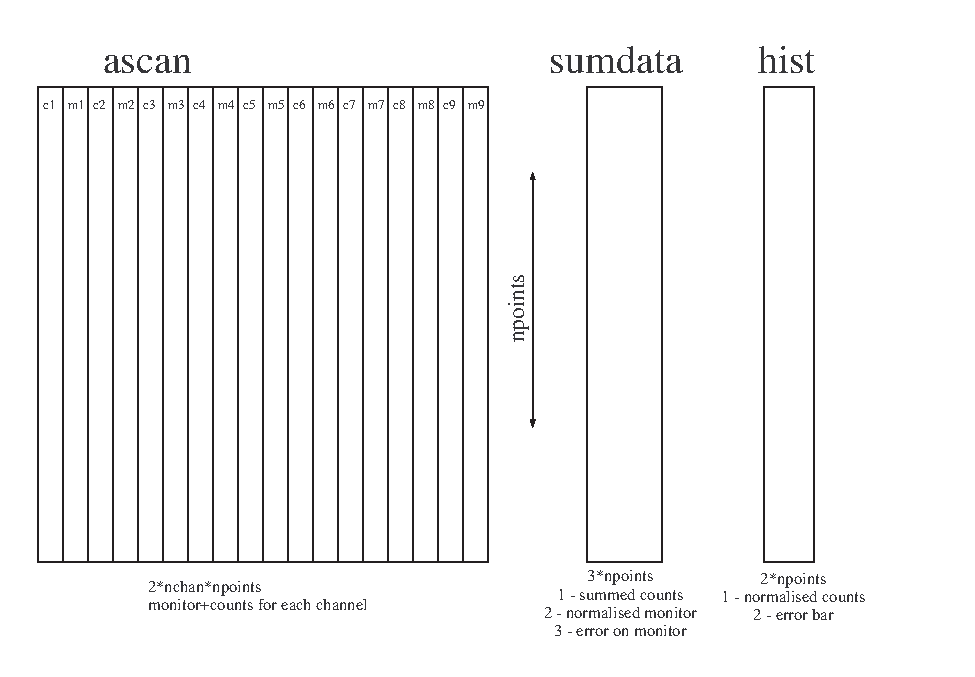
\includegraphics{bigarrays.eps}
  \caption{Illustration of the large arrays in use in the programs
  and their intended memory contents.}
  \label{fig:bigarrays}
\end{figure}

\subsection{Some functions for binning}
The bins are to have 2$\theta$ centers at thlow, tthlow + step, 
tthlow + 2$\times$step, etc.
Functions for working out which bin a particular 2$\theta$ value falls into 
along with the limits and centre of the bin are given here. 
An integer is whic used for accessing the ascan array is used to label
each bin, 
these will start at tthlow and end at tthhigh, returning
-1 for a 2$\theta$ value which is out of range. 
Figure~\ref{fig:bindef} will
hopefully make it clearer what these functions are doing.

\begin{figure}[tb]
  \centering
  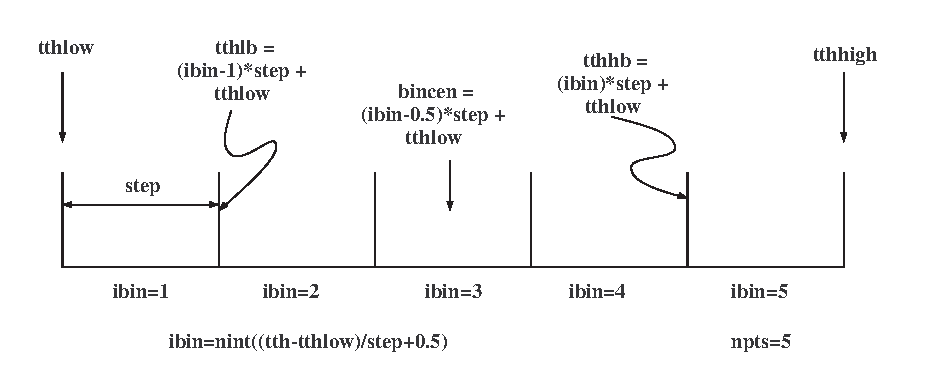
\includegraphics{bindef.eps}
  \caption{Illustration of the bin definitions. \code{ibin} calculates an
  integer to be assigned to any particular bin and the other functions 
  find the limits and center of a bin labelled by ibin.}
  \label{fig:bindef}
\end{figure}

\code{ibin} returns the integer bin number for a particular bin.

\begin{flushleft} \small
\begin{minipage}{\linewidth}\label{scrap23}\raggedright\small
\NWtarget{nuweb20a}{} $\langle\,${\it ibin}\nobreak\ {\footnotesize {20a}}$\,\rangle\equiv$
\vspace{-1ex}
\begin{list}{}{} \item
\mbox{}\verb@      integer(kind=4) function ibin(tth)@\\
\mbox{}\verb@      real(kind=8), intent(in) :: tth@\\
\mbox{}\verb@      real(kind=8)::x@\\
\mbox{}\verb@      if(tth.ge.tthlow .and. tth.le.tthhigh) then@\\
\mbox{}\verb@        x=(tth-tthlow)/step+0.5d0@\\
\mbox{}\verb@        ibin=int(x) @\\
\mbox{}\verb@      else ;  ibin=-1 ; endif       ! Out of range for this ascan array@\\
\mbox{}\verb@      return ; end function ibin                                             @{\NWsep}
\end{list}
\vspace{-1.5ex}
\footnotesize
\begin{list}{}{\setlength{\itemsep}{-\parsep}\setlength{\itemindent}{-\leftmargin}}
\item \NWtxtMacroRefIn\ \NWlink{nuweb28}{28}.

\item{}
\end{list}
\end{minipage}\vspace{4ex}
\end{flushleft}
The upper 2$\theta$ limit for a bin is to be given by a function tthhb: 

\begin{flushleft} \small
\begin{minipage}{\linewidth}\label{scrap24}\raggedright\small
\NWtarget{nuweb20b}{} $\langle\,${\it tthhb}\nobreak\ {\footnotesize {20b}}$\,\rangle\equiv$
\vspace{-1ex}
\begin{list}{}{} \item
\mbox{}\verb@      real(kind=8) function tthhb(n)@\\
\mbox{}\verb@      integer(kind=4), intent(in) :: n@\\
\mbox{}\verb@      integer(kind=4)nplusone@\\
\mbox{}\verb@      nplusone=n+1@\\
\mbox{}\verb@      tthhb=tthlb(nplusone)@\\
\mbox{}\verb@      return; end function tthhb                                             @{\NWsep}
\end{list}
\vspace{-1.5ex}
\footnotesize
\begin{list}{}{\setlength{\itemsep}{-\parsep}\setlength{\itemindent}{-\leftmargin}}
\item \NWtxtMacroRefIn\ \NWlink{nuweb28}{28}.

\item{}
\end{list}
\end{minipage}\vspace{4ex}
\end{flushleft}
The lower 2$\theta$ limit for a bin is to be given by a function tthlb:
\begin{flushleft} \small
\begin{minipage}{\linewidth}\label{scrap25}\raggedright\small
\NWtarget{nuweb21a}{} $\langle\,${\it tthlb}\nobreak\ {\footnotesize {21a}}$\,\rangle\equiv$
\vspace{-1ex}
\begin{list}{}{} \item
\mbox{}\verb@      real(kind=8) function tthlb(n)@\\
\mbox{}\verb@      integer(kind=4), intent(in) :: n@\\
\mbox{}\verb@      tthlb = (real(n,8)-0.5d0)*step + tthlow@\\
\mbox{}\verb@      return; end function tthlb                                      @{\NWsep}
\end{list}
\vspace{-1.5ex}
\footnotesize
\begin{list}{}{\setlength{\itemsep}{-\parsep}\setlength{\itemindent}{-\leftmargin}}
\item \NWtxtMacroRefIn\ \NWlink{nuweb28}{28}.

\item{}
\end{list}
\end{minipage}\vspace{4ex}
\end{flushleft}
The center of the bin is given by a function bincen:
\begin{flushleft} \small
\begin{minipage}{\linewidth}\label{scrap26}\raggedright\small
\NWtarget{nuweb21b}{} $\langle\,${\it bincen}\nobreak\ {\footnotesize {21b}}$\,\rangle\equiv$
\vspace{-1ex}
\begin{list}{}{} \item
\mbox{}\verb@      real(kind=8) function bincen(n)@\\
\mbox{}\verb@      integer(kind=4), intent(in) :: n@\\
\mbox{}\verb@      bincen = real(n,8)*step + tthlow@\\
\mbox{}\verb@      return; end function bincen                                     @{\NWsep}
\end{list}
\vspace{-1.5ex}
\footnotesize
\begin{list}{}{\setlength{\itemsep}{-\parsep}\setlength{\itemindent}{-\leftmargin}}
\item \NWtxtMacroRefIn\ \NWlink{nuweb28}{28}.

\item{}
\end{list}
\end{minipage}\vspace{4ex}
\end{flushleft}
Checking the parameters before initialising the ascan array should avoid a lot
of problems and also allow us to ensure that there is always a bin centered on
2$\theta=0$. 
We check tthlow and tthhigh and adjust them to be the edges of the bins
we assume they were aiming at, given a bin centred at 0, and also we check 
the stepsize is physically reasonable. 
The diffractometer is sensitive to angular displacements of
$5 \times 10^{-5}$, so any binsize smaller than that would be a bit silly.

\begin{flushleft} \small
\begin{minipage}{\linewidth}\label{scrap27}\raggedright\small
\NWtarget{nuweb22}{} $\langle\,${\it checkrebinpars}\nobreak\ {\footnotesize {22}}$\,\rangle\equiv$
\vspace{-1ex}
\begin{list}{}{} \item
\mbox{}\verb@      subroutine checkrebinpars@\\
\mbox{}\verb@      real(kind=8) :: x@\\
\mbox{}\verb@      if ((units.ne.'T').and. (.not. wavelength_set) ) return@\\
\mbox{}\verb@      if(step.lt.aminstep .and. (units.eq.'T'))then@\\
\mbox{}\verb@       write(*,'(a,G12.4)')'Step is a bit small, resetting to ',aminstep@\\
\mbox{}\verb@       step=aminstep@\\
\mbox{}\verb@       user_step = step@\\
\mbox{}\verb@      endif@\\
\mbox{}\verb@      x=tthlow/step @\\
\mbox{}\verb@      tthlow=real(int(x),8)*step@\\
\mbox{}\verb@      x=(tthhigh-tthlow)/step@\\
\mbox{}\verb@      npts=int(x) @\\
\mbox{}\verb@      tthhigh=tthhb(npts)@\\
\mbox{}\verb@      if (units .eq. 'T') then@\\
\mbox{}\verb@      write(*,'(3(G12.5,a),G12.5)')tthlow,' < tth < ',tthhigh,            &@\\
\mbox{}\verb@     &' step=',step,' npts=',npts@\\
\mbox{}\verb@      endif@\\
\mbox{}\verb@      if (units.eq.'Q') then@\\
\mbox{}\verb@      write(*,'(3(G12.5,a),G12.5)')tthlow,' < 2pi/d < ',tthhigh,          &@\\
\mbox{}\verb@     &' step=',step,' npts=',npts@\\
\mbox{}\verb@      endif@\\
\mbox{}\verb@      if (units.eq.'R') then@\\
\mbox{}\verb@      write(*,'(3(G12.5,a),G12.5)')tthlow,' < Q^2 < ',tthhigh,            &@\\
\mbox{}\verb@     &' step=',step,' npts=',npts@\\
\mbox{}\verb@      endif@\\
\mbox{}\verb@      return@\\
\mbox{}\verb@      end subroutine checkrebinpars                                          @{\NWsep}
\end{list}
\vspace{-1.5ex}
\footnotesize
\begin{list}{}{\setlength{\itemsep}{-\parsep}\setlength{\itemindent}{-\leftmargin}}
\item \NWtxtMacroRefIn\ \NWlink{nuweb28}{28}.

\item{}
\end{list}
\end{minipage}\vspace{4ex}
\end{flushleft}
\subsection{Initialisation}
\label{rebin:init}
Some of the data will need to be initialised before any rebinning can be
carried out. Traditionally a file called "temp.res" is used to hold the 
detector offsets. We will also need to decide upon the scan range and 
stepsize and allocate an array to hold the data.

\begin{flushleft} \small
\begin{minipage}{\linewidth}\label{scrap28}\raggedright\small
\NWtarget{nuweb23}{} $\langle\,${\it initialiserebin}\nobreak\ {\footnotesize {23}}$\,\rangle\equiv$
\vspace{-1ex}
\begin{list}{}{} \item
\mbox{}\verb@      subroutine initialiserebin@\\
\mbox{}\verb@      integer(kind=4) :: ierr, i@\\
\mbox{}\verb@      real(kind=8) :: junk@\\
\mbox{}\verb@!      real :: time1, time2@\\
\mbox{}\verb@! constants to machine precision@\\
\mbox{}\verb@      four_pi = 8.0d0*asin(1.0d0)@\\
\mbox{}\verb@      pi_over_360 = asin(1.0d0)/180.0d0@\\
\mbox{}\verb@! default values@\\
\mbox{}\verb@@\hbox{$\langle\,${\it offsetdefaults}\nobreak\ {\footnotesize \NWlink{nuweb18}{18}}$\,\rangle$}\verb@@\\
\mbox{}\verb@      open(unit=16,file='temp.res',form='FORMATTED',                    &@\\
\mbox{}\verb@     & access='SEQUENTIAL', status='OLD', iostat=ierr)@\\
\mbox{}\verb@      if(ierr.eq.0)then@\\
\mbox{}\verb@         do i=1,nchannel@\\
\mbox{}\verb@! Should clarify policy on whether to read/use these?@\\
\mbox{}\verb@          read(16,*,err=10,end=12)offset(i),mult(i),multerr(i),junk@\\
\mbox{}\verb@         enddo@\\
\mbox{}\verb@! Report temp.res found and read in         @\\
\mbox{}\verb@         write(*,'(a)')'temp.res file found and read in'@\\
\mbox{}\verb@         tempres=.true.@\\
\mbox{}\verb@        goto 11@\\
\mbox{}\verb@      endif@\\
\mbox{}\verb@10    write(*,'(a)')'Not able to read temp.res file,'                 @\\
\mbox{}\verb@      write(*,'(a)')'You need this file for the detector calibration'@\\
\mbox{}\verb@      write(*,'(a)')'Please copy this file to the current directory'@\\
\mbox{}\verb@      write(*,'(a)')' eg:  " cp ~/temp.res ." '@\\
\mbox{}\verb@      stop@\\
\mbox{}\verb@12    write(*,'(a)')'Reached end of temp.res file early?'@\\
\mbox{}\verb@11    close(16)@\\
\mbox{}\verb@! two theta low, two theta high, step and that npts is correct@\\
\mbox{}\verb@      if ((units.eq.'T') .or. wavelength_set) call unit_lims@\\
\mbox{}\verb@      return ; end subroutine initialiserebin@\\
\mbox{}\verb@@\\
\mbox{}\verb@      subroutine rebinallocate@\\
\mbox{}\verb@      implicit none@\\
\mbox{}\verb@      integer ierr@\\
\mbox{}\verb@      if( allocated(ascan) ) deallocate(ascan) ! can reset@\\
\mbox{}\verb@      allocate(ascan(nchannel*2,npts),stat=ierr)@\\
\mbox{}\verb@      if(ierr.ne.0)stop 'Memory allocation error'@\\
\mbox{}\verb@!      call cpu_time(time1)@\\
\mbox{}\verb@      ascan=0.0d0   ! Clear any junk  @\\
\mbox{}\verb@!      call cpu_time(time2)@\\
\mbox{}\verb@!      write(*,*)'Time taken to zero array =',time2-time1,'/s'@\\
\mbox{}\verb@      return ; end subroutine rebinallocate      @\\
\mbox{}\verb@      @{\NWsep}
\end{list}
\vspace{-1.5ex}
\footnotesize
\begin{list}{}{\setlength{\itemsep}{-\parsep}\setlength{\itemindent}{-\leftmargin}}
\item \NWtxtMacroRefIn\ \NWlink{nuweb28}{28}.

\item{}
\end{list}
\end{minipage}\vspace{4ex}
\end{flushleft}
The commented out lines are used to find out if the program is thrashing 
the hard disk. If the time taken to zero the array is more than a small
fraction of a second the program will run very slowly. This happens if
it is running on a computer which has run out of RAM and is using the
hard disk for virtual memory.

\subsection{The binning algorithm}

Finally we get to the guts of the thing, the actual rebinning algorithm. 
This will eventually take a line of entries from the SPEC file and assign 
them to bins. 
Some explanation of SPEC files is required here. 
Figure~\ref{fig:bin} shows a graphical representation of the data in the 
SPEC file. 
The starting 2$\theta$ position is given in the file header and then datalines contain the current value of 2$\theta$ and the number of counts which
have arrived at the detector since the last dataline.

\begin{figure}[tb]
  \centering
  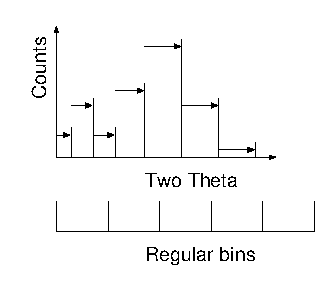
\includegraphics{bin.eps}
  \caption{Illustration of the SPEC file contents, the initial two theta value
 is in the file header, subsequent lines record the current two theta value
 and counts arriving since the last line, indicated by the arrows.}
  \label{fig:bin}
\end{figure}

For processing a single line of data we will need to know the value of 
2$\theta$ from the previous line (or header) and the current 2$\theta$ value. 
The counts are then assumed to have been arriving uniformly between those two
values and are apportioned to bins accordingly. 
The bins are designated by their borders and the convention will be taken that there is always a bin centred on zero. 
The algorithm will proceed as follows:
\begin{enumerate}
\item Obtain the lower and upper of the 2$\theta$ detector positions, 
2$\theta_l$ and 2$\theta_u$
\item Identify the bin into which this 2$\theta_l$ falls and note the upper
      limit of the bin 2$\theta_b$
\item If the upper detector position is also within this bin put all the counts
     in this bin and exit
\item If the upper position is in the next bin apportion the counts to the two
     bins so the lower bins gets the fraction 
      $\frac{2\theta_{b}-2\theta_l}{2\theta_{u}-2\theta_l}$
      and put the rest in the upper bin and exit.
\item Otherwise put the fraction 
        $\frac{2\theta_{b}-2\theta_l}{2\theta_{u}-2\theta_l}$
      in the lower bin, the corresponding fraction in the topmost bin
      and split the rest of the counts amongst the rest of the bins. exit.
\end{enumerate}

Figure~\ref{fig:binalg} is intended to illuminate this process, in case 
the text wasn't clear.
\begin{figure}[tb]
  \centering
  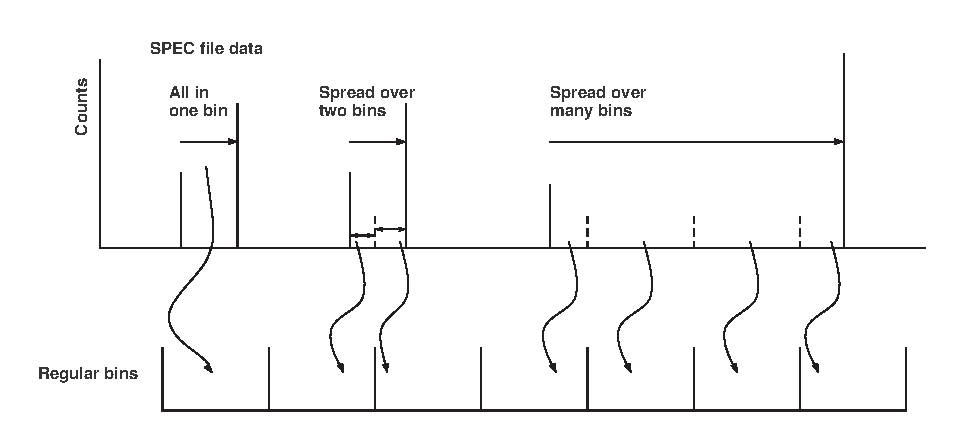
\includegraphics{binalg.eps}
  \caption{Illustration of the binning procedure. Counts are assigned to bins
   assuming they arrived uniformly during the sampling time.}
  \label{fig:binalg}
\end{figure}

The following subroutine takes an upper and lower 2$\theta$, a number of 
counts, and a channel number and places these counts into the appropriate bin.

\begin{flushleft} \small
\begin{minipage}{\linewidth}\label{scrap29}\raggedright\small
\NWtarget{nuweb25}{} $\langle\,${\it bin}\nobreak\ {\footnotesize {25}}$\,\rangle\equiv$
\vspace{-1ex}
\begin{list}{}{} \item
\mbox{}\verb@      subroutine bin(tth1,tth2,cts,ichan)@\\
\mbox{}\verb@! tthh & tthl are the high & low two thetas from the SPEC file@\\
\mbox{}\verb@! cts is the number of counts and ichan is the column to use in ascan@\\
\mbox{}\verb@      real(kind=8), intent(in) :: tth1, tth2, cts@\\
\mbox{}\verb@      integer(kind=4), intent(in) :: ichan@\\
\mbox{}\verb@      integer(kind=4) :: ibl, ibh, j@\\
\mbox{}\verb@      real(kind=8) :: frac, tthh, tthl@\\
\mbox{}\verb@!      tthl=min(tth1,tth2)                       ! Ensures ascending data@\\
\mbox{}\verb@!      tthh=max(tth1,tth2)    ! strange bug on Fe3O4 exp??@\\
\mbox{}\verb@      if(tth1 .ge. tth2)then@\\
\mbox{}\verb@        tthl=tth2; tthh=tth1@\\
\mbox{}\verb@      else@\\
\mbox{}\verb@        tthl=tth1; tthh=tth2@\\
\mbox{}\verb@      endif@\\
\mbox{}\verb@      ibl = ibin(tthl)                              ! Bin of lower point@\\
\mbox{}\verb@      ibh = ibin(tthh)                              ! Bin of upper point@\\
\mbox{}\verb@      if ((ibl.le.0).or.(ibh.lt.ibl).or.(ibh.gt.npts))return     ! error   @\\
\mbox{}\verb@      if ( ibh .eq. ibl) then                           ! All in one bin@\\
\mbox{}\verb@         ascan(ichan,ibl) = ascan(ichan,ibl) + cts@\\
\mbox{}\verb@         return@\\
\mbox{}\verb@      elseif ( ibh .eq. ibl+1) then               ! Spread over two bins@\\
\mbox{}\verb@         frac=(tthhb(ibl)-tthl)/(tthh-tthl)          ! Fraction in bin 1@\\
\mbox{}\verb@         ascan(ichan,ibl)=ascan(ichan,ibl) + cts*frac@\\
\mbox{}\verb@         ascan(ichan,ibh)=ascan(ichan,ibh) + cts*(1.0d0-frac)@\\
\mbox{}\verb@         return@\\
\mbox{}\verb@      else@\\
\mbox{}\verb@         frac=(tthhb(ibl)-tthl)/(tthh-tthl)          ! Fraction in bin 1@\\
\mbox{}\verb@         ascan(ichan,ibl)=ascan(ichan,ibl) + cts*frac@\\
\mbox{}\verb@         frac=(tthh-tthlb(ibh))/(tthh-tthl)       ! Fraction in last bin @\\
\mbox{}\verb@         ascan(ichan,ibh)=ascan(ichan,ibh) + cts*frac @\\
\mbox{}\verb@         frac= step/(tthh-tthl)                ! Fraction in middle bins@\\
\mbox{}\verb@         do j = ibl+1,ibh-1,1@\\
\mbox{}\verb@           ascan(ichan,j)=ascan(ichan,j) + cts*frac @\\
\mbox{}\verb@         enddo@\\
\mbox{}\verb@         return@\\
\mbox{}\verb@      endif@\\
\mbox{}\verb@      end subroutine bin                                                     @{\NWsep}
\end{list}
\vspace{-1.5ex}
\footnotesize
\begin{list}{}{\setlength{\itemsep}{-\parsep}\setlength{\itemindent}{-\leftmargin}}
\item \NWtxtMacroRefIn\ \NWlink{nuweb28}{28}.

\item{}
\end{list}
\end{minipage}\vspace{4ex}
\end{flushleft}
Finally we create a routine that takes a line of data from a SPEC files 
and uses the rebinning code above to process the entire line of entries. 
The detector offset must be added to the 2$\theta$ value for each detector
before it can be binned. 
The specification of the contents of the ascan array is decided here, column 1
will correspond to detector 1, column 2 is a monitor column for detector 1 and 
so on.
Users of the routine must supply a high and low 2$\theta$ value along with
a set of counts and a monitor column.

\begin{flushleft} \small
\begin{minipage}{\linewidth}\label{scrap30}\raggedright\small
\NWtarget{nuweb26}{} $\langle\,${\it processline}\nobreak\ {\footnotesize {26}}$\,\rangle\equiv$
\vspace{-1ex}
\begin{list}{}{} \item
\mbox{}\verb@      subroutine processline(tth1,tth2,cts,n,ctsmon)@\\
\mbox{}\verb@      real(kind=8), intent(in) :: tth1, tth2, ctsmon@\\
\mbox{}\verb@      integer(kind=4), intent(in) :: n@\\
\mbox{}\verb@      real(kind=8), intent(in), dimension(n) :: cts@\\
\mbox{}\verb@      integer(kind=4) :: i, ich@\\
\mbox{}\verb@      real(kind=8) :: tthh, tthl@\\
\mbox{}\verb@      do i = 1,n@\\
\mbox{}\verb@        if(logexdet(i).eq.1)cycle ! skip if excluded completely@\\
\mbox{}\verb@        if(userandomstart.and.rstchan(i).and.(tth2.lt.randomval))cycle@\\
\mbox{}\verb@        if(userandomend.and.renchan(i).and.(tth2.gt.randomvalend))cycle@\\
\mbox{}\verb@        tthl = tth1 - offset(i)@\\
\mbox{}\verb@        tthh = tth2 - offset(i)@\\
\mbox{}\verb@        if(logexdet(i).eq.2)then@\\
\mbox{}\verb@! Is this an excluded region for this channel@\\
\mbox{}\verb@          if(led(i,tthl,tthh))cycle  @\\
\mbox{}\verb@        endif@\\
\mbox{}\verb@        tthl = convert_unit_function( tthl )@\\
\mbox{}\verb@        tthh = convert_unit_function( tthh )@\\
\mbox{}\verb@        ich = 2*i-1@\\
\mbox{}\verb@        call bin(tthl,tthh,cts(i),ich)@\\
\mbox{}\verb@        ich = 2*i@\\
\mbox{}\verb@        call bin(tthl,tthh,ctsmon,ich)@\\
\mbox{}\verb@        sumtotal(i)=sumtotal(i)+cts(i)@\\
\mbox{}\verb@      enddo@\\
\mbox{}\verb@      sumtotalmon=sumtotalmon+ctsmon@\\
\mbox{}\verb@      return@\\
\mbox{}\verb@      end subroutine processline                                             @{\NWsep}
\end{list}
\vspace{-1.5ex}
\footnotesize
\begin{list}{}{\setlength{\itemsep}{-\parsep}\setlength{\itemindent}{-\leftmargin}}
\item \NWtxtMacroRefIn\ \NWlink{nuweb28}{28}.

\item{}
\end{list}
\end{minipage}\vspace{4ex}
\end{flushleft}
Checking if a particular channel is excluded in a particular two theta interval
needs the function \code{led}. It just runs through a stored version of the 
excluded region file to return true or false.

\begin{flushleft} \small
\begin{minipage}{\linewidth}\label{scrap31}\raggedright\small
\NWtarget{nuweb27}{} $\langle\,${\it led}\nobreak\ {\footnotesize {27}}$\,\rangle\equiv$
\vspace{-1ex}
\begin{list}{}{} \item
\mbox{}\verb@      logical function led(ic,xl,xh)@\\
\mbox{}\verb@      use specfiles@\\
\mbox{}\verb@      integer(kind=4),intent(in) :: ic@\\
\mbox{}\verb@      real(kind=8),intent(in) :: xl, xh@\\
\mbox{}\verb@      integer(kind=4)i@\\
\mbox{}\verb@      if(.not.allocated(iexarray).or. .not. allocated(exarray)) then@\\
\mbox{}\verb@! oh dear, function should never have been called@\\
\mbox{}\verb@        write(*,'(a)')'Bug in program, bailing out, sorry!'@\\
\mbox{}\verb@        write(*,'(a)')'Please mail a bug report to wright@{\tt @}\verb@esrf.fr'@\\
\mbox{}\verb@        stop@\\
\mbox{}\verb@      endif@\\
\mbox{}\verb@      led=.false.@\\
\mbox{}\verb@      do i=1,iexrc@\\
\mbox{}\verb@        if((iexarray(i)+1).eq.ic)then !  found the right line@\\
\mbox{}\verb@          if(int(exarray(i,3)).lt.1)then@\\
\mbox{}\verb@           if(xl.gt.exarray(i,1) .and.xl.lt.exarray(i,2))led=.true.@\\
\mbox{}\verb@           if(xh.gt.exarray(i,1) .and.xh.lt.exarray(i,2))led=.true.@\\
\mbox{}\verb@          else@\\
\mbox{}\verb@           if(xl.gt.exarray(i,1) .and.xl.lt.exarray(i,2) .and. &@\\
\mbox{}\verb@     & iscan.eq.int(exarray(i,3)))led=.true.@\\
\mbox{}\verb@           if(xh.gt.exarray(i,1) .and.xh.lt.exarray(i,2) .and. &@\\
\mbox{}\verb@     & iscan.eq.int(exarray(i,3)))led=.true.@\\
\mbox{}\verb@          endif@\\
\mbox{}\verb@        endif@\\
\mbox{}\verb@      enddo@\\
\mbox{}\verb@      return@\\
\mbox{}\verb@      end function led                                                  @{\NWsep}
\end{list}
\vspace{-1.5ex}
\footnotesize
\begin{list}{}{\setlength{\itemsep}{-\parsep}\setlength{\itemindent}{-\leftmargin}}
\item \NWtxtMacroRefIn\ \NWlink{nuweb28}{28}.

\item{}
\end{list}
\end{minipage}\vspace{4ex}
\end{flushleft}
\subsection{A rebinning module}
The data and functions created so far should be all that we need to carry out
the rebinning process. 
They are collected together for in module so they can be
used elsewhere.
\begin{flushleft} \small
\begin{minipage}{\linewidth}\label{scrap32}\raggedright\small
\NWtarget{nuweb28}{} $\langle\,${\it rebin}\nobreak\ {\footnotesize {28}}$\,\rangle\equiv$
\vspace{-1ex}
\begin{list}{}{} \item
\mbox{}\verb@      module rebin@\\
\mbox{}\verb@@\hbox{$\langle\,${\it OFFSET}\nobreak\ {\footnotesize \NWlink{nuweb17}{17}}$\,\rangle$}\verb@@\\
\mbox{}\verb@@\hbox{$\langle\,${\it SCAN}\nobreak\ {\footnotesize \NWlink{nuweb19}{19}}$\,\rangle$}\verb@@\\
\mbox{}\verb@      real(kind=8) :: sumtotal(nchan), sumtotalmon, minmon=1.0d0@\\
\mbox{}\verb@      real(kind=8) :: winhigh,winlow,winhighread,winlowread@\\
\mbox{}\verb@      integer(kind=4) :: wincol@\\
\mbox{}\verb@      real(kind=8) :: minrenormsig=5.0@\\
\mbox{}\verb@      real(kind=8) :: randomstart = 0, randomval=0@\\
\mbox{}\verb@      real(kind=8) :: randomend = 0, randomvalend=0@\\
\mbox{}\verb@      character(len=90) :: wincnt@\\
\mbox{}\verb@      logical :: winlog=.false. @\\
\mbox{}\verb@      logical :: userandomstart = .false.@\\
\mbox{}\verb@      logical :: rstchan( nchan ) = .false.@\\
\mbox{}\verb@      logical :: userandomend = .false.@\\
\mbox{}\verb@      logical :: renchan( nchan ) = .false.@\\
\mbox{}\verb@      logical :: wavelength_set = .false.@\\
\mbox{}\verb@      real(kind=8) :: wavelength=0.0d0@\\
\mbox{}\verb@      ! T = Two theta@\\
\mbox{}\verb@      ! Q = 4 * pi * sin( two_theta * pi / 360.0 ) / wavelength@\\
\mbox{}\verb@      ! R = [q squared] = Q * Q@\\
\mbox{}\verb@      character(len=1) :: units = 'T'@\\
\mbox{}\verb@      real(kind=8) :: four_pi, pi_over_360@\\
\mbox{}\verb@      contains@\\
\mbox{}\verb@@\hbox{$\langle\,${\it ibin}\nobreak\ {\footnotesize \NWlink{nuweb20a}{20a}}$\,\rangle$}\verb@@\\
\mbox{}\verb@@\hbox{$\langle\,${\it tthhb}\nobreak\ {\footnotesize \NWlink{nuweb20b}{20b}}$\,\rangle$}\verb@@\\
\mbox{}\verb@@\hbox{$\langle\,${\it tthlb}\nobreak\ {\footnotesize \NWlink{nuweb21a}{21a}}$\,\rangle$}\verb@@\\
\mbox{}\verb@@\hbox{$\langle\,${\it bincen}\nobreak\ {\footnotesize \NWlink{nuweb21b}{21b}}$\,\rangle$}\verb@@\\
\mbox{}\verb@@\hbox{$\langle\,${\it checkrebinpars}\nobreak\ {\footnotesize \NWlink{nuweb22}{22}}$\,\rangle$}\verb@@\\
\mbox{}\verb@@\hbox{$\langle\,${\it initialiserebin}\nobreak\ {\footnotesize \NWlink{nuweb23}{23}}$\,\rangle$}\verb@@\\
\mbox{}\verb@@\hbox{$\langle\,${\it bin}\nobreak\ {\footnotesize \NWlink{nuweb25}{25}}$\,\rangle$}\verb@@\\
\mbox{}\verb@@\hbox{$\langle\,${\it processline}\nobreak\ {\footnotesize \NWlink{nuweb26}{26}}$\,\rangle$}\verb@@\\
\mbox{}\verb@@\hbox{$\langle\,${\it led}\nobreak\ {\footnotesize \NWlink{nuweb27}{27}}$\,\rangle$}\verb@@\\
\mbox{}\verb@@\hbox{$\langle\,${\it window}\nobreak\ {\footnotesize \NWlink{nuweb37}{37}}$\,\rangle$}\verb@@\\
\mbox{}\verb@@\hbox{$\langle\,${\it convertunitfunction}\nobreak\ {\footnotesize \NWlink{nuweb30}{30}}$\,\rangle$}\verb@@\\
\mbox{}\verb@@\hbox{$\langle\,${\it random}\nobreak\ {\footnotesize \NWlink{nuweb136a}{136a}}$\,\rangle$}\verb@@\\
\mbox{}\verb@      end module rebin                                                       @{\NWsep}
\end{list}
\vspace{-1.5ex}
\footnotesize
\begin{list}{}{\setlength{\itemsep}{-\parsep}\setlength{\itemindent}{-\leftmargin}}
\item \NWtxtMacroRefIn\ \NWlink{nuweb31a}{31a}\NWlink{nuweb32}{, 32}\NWlink{nuweb40a}{, 40a}\NWlink{nuweb57b}{, 57b}\NWlink{nuweb86b}{, 86b}\NWlink{nuweb89}{, 89}\NWlink{nuweb91}{, 91}.

\item{}
\end{list}
\end{minipage}\vspace{4ex}
\end{flushleft}
Now we need some information from the user on the command line. Namely,
the unit to use (two theta remains as a default) and the wavelength as 
an option

\begin{flushleft} \small
\begin{minipage}{\linewidth}\label{scrap33}\raggedright\small
\NWtarget{nuweb29}{} $\langle\,${\it unitsoptions}\nobreak\ {\footnotesize {29}}$\,\rangle\equiv$
\vspace{-1ex}
\begin{list}{}{} \item
\mbox{}\verb@@\\
\mbox{}\verb@! These will end up in the useroptions module@\\
\mbox{}\verb@!        case('wvl')  call setwavelength(string)@\\
\mbox{}\verb@!@\\
\mbox{}\verb@      subroutine setwavelength(s)@\\
\mbox{}\verb@      use rebin@\\
\mbox{}\verb@      character(len=*), intent(in) :: s@\\
\mbox{}\verb@      if(s(1:5).eq.'wvln=')read(s(6:len_trim(s)),*,err=1)wavelength@\\
\mbox{}\verb@      wavelength_set = .true.@\\
\mbox{}\verb@      write(*,*)'Using wavelength of ',wavelength@\\
\mbox{}\verb@      return@\\
\mbox{}\verb@1     write(*,*)'Error reading wavelength',s@\\
\mbox{}\verb@      stop@\\
\mbox{}\verb@      end subroutine setwavelength@\\
\mbox{}\verb@!@\\
\mbox{}\verb@!        case('uni')  call setunits(string)@\\
\mbox{}\verb@      subroutine setunits(s)@\\
\mbox{}\verb@      use rebin@\\
\mbox{}\verb@      character(len=*), intent(in) :: s@\\
\mbox{}\verb@!                      12345678@\\
\mbox{}\verb@      if( s(1:8) .eq. 'units=Q2' ) then@\\
\mbox{}\verb@          units = 'R'@\\
\mbox{}\verb@          write(*,*)'Binning into Q^2 = 16.pi^2.sin^2(theta)/wavelength^2'@\\
\mbox{}\verb@          return@\\
\mbox{}\verb@      endif@\\
\mbox{}\verb@!                      1234567@\\
\mbox{}\verb@      if( s(1:7) .eq. 'units=Q' ) then@\\
\mbox{}\verb@          units = 'Q'@\\
\mbox{}\verb@          write(*,*)'Binning into Q = 4.pi.sin(theta)/wavelength'@\\
\mbox{}\verb@          return@\\
\mbox{}\verb@      endif@\\
\mbox{}\verb@@\\
\mbox{}\verb@      write(*,*)'Did not understand your option',s@\\
\mbox{}\verb@      write(*,*)'Use nothing for twotheta, units=Q or units=Q2'@\\
\mbox{}\verb@      stop @\\
\mbox{}\verb@      end subroutine setunits@\\
\mbox{}\verb@@{\NWsep}
\end{list}
\vspace{-1.5ex}
\footnotesize
\begin{list}{}{\setlength{\itemsep}{-\parsep}\setlength{\itemindent}{-\leftmargin}}
\item \NWtxtMacroRefIn\ \NWlink{nuweb87a}{87a}.

\item{}
\end{list}
\end{minipage}\vspace{4ex}
\end{flushleft}
This module now contains everything we will need for rebinning our data.

\subsection{Converting to another unit }

March 2009, some people want to bin into constant steps in Q, 

 \[ Q = \frac{4\pi \sin{\theta} }{\lambda}  \]

We get the wavelength, $\lambda$ either from the command line,
or from the header of the scans Q(4) fortran or Q[3] in C. 

For completeness we'll do Q squared at the same time. Might be interesting
for plotting data on a log scale (thermal factors go as q squared).

D-spacing offers
an exciting possibility for dividing by zero, so it is skipped for now.

\begin{flushleft} \small
\begin{minipage}{\linewidth}\label{scrap34}\raggedright\small
\NWtarget{nuweb30}{} $\langle\,${\it convertunitfunction}\nobreak\ {\footnotesize {30}}$\,\rangle\equiv$
\vspace{-1ex}
\begin{list}{}{} \item
\mbox{}\verb@@\\
\mbox{}\verb@      real(kind=8) function convert_unit_function( x )@\\
\mbox{}\verb@      real(kind=8), intent(in) :: x@\\
\mbox{}\verb@      real(kind=8) :: qt@\\
\mbox{}\verb@      select case((units))@\\
\mbox{}\verb@        case('T') ! Two theta, do nothing@\\
\mbox{}\verb@           convert_unit_function = x@\\
\mbox{}\verb@           return@\\
\mbox{}\verb@        case('Q') ! Q - constants from initialise_rebin@\\
\mbox{}\verb@           convert_unit_function = four_pi*sin(x*pi_over_360)/wavelength@\\
\mbox{}\verb@           return@\\
\mbox{}\verb@        case('R') ! Q^2 @\\
\mbox{}\verb@           qt = four_pi * sin( x * pi_over_360 )/wavelength@\\
\mbox{}\verb@! use a signed quantity@\\
\mbox{}\verb@!        write(*,*)qt,qt*qt,SIGN( qt * qt , qt ),x@\\
\mbox{}\verb@           convert_unit_function = sign( qt * qt , qt )@\\
\mbox{}\verb@           return@\\
\mbox{}\verb@        case default@\\
\mbox{}\verb@           convert_unit_function = x@\\
\mbox{}\verb@           return@\\
\mbox{}\verb@      end select@\\
\mbox{}\verb@      return@\\
\mbox{}\verb@      end function convert_unit_function@\\
\mbox{}\verb@!@\\
\mbox{}\verb@!@\\
\mbox{}\verb@! To be called once per scan - picks up wavelength from command line@\\
\mbox{}\verb@      subroutine convert_unit_setupQ( Q )@\\
\mbox{}\verb@! from rebin module :::: logical :: wavelength_set = .false.@\\
\mbox{}\verb@      real(kind=8), dimension(60), intent(in) :: Q@\\
\mbox{}\verb@      if ( (units .eq. 'T') .or. wavelength_set) then@\\
\mbox{}\verb@         return@\\
\mbox{}\verb@      endif @\\
\mbox{}\verb@      if( Q(4) .gt. 1.0E-15 ) then@\\
\mbox{}\verb@          wavelength = Q(4)@\\
\mbox{}\verb@! Assume always the same for all scans:@\\
\mbox{}\verb@          write(*,*)@\\
\mbox{}\verb@          write(*,*)'Got wavelength',wavelength,'from spec file Q[3]'@\\
\mbox{}\verb@          wavelength_set = .true.@\\
\mbox{}\verb@      endif@\\
\mbox{}\verb@! Check for errors@\\
\mbox{}\verb@! let them have Angstroms as meters (1e-11) @\\
\mbox{}\verb@      if ((wavelength .lt. 1.0E-15) .and. (units .ne. 'T') ) then@\\
\mbox{}\verb@        write(*,*)'Your wavelength is a bit small ',wavelength @\\
\mbox{}\verb@        write(*,*)'Giving up, try putting wvln=1.234 on command line'@\\
\mbox{}\verb@        stop@\\
\mbox{}\verb@      endif@\\
\mbox{}\verb@!      write(*,*)'calling setupQ from convert_unit_setupQ'@\\
\mbox{}\verb@      call unit_lims()@\\
\mbox{}\verb@      return@\\
\mbox{}\verb@      end subroutine convert_unit_setupQ@\\
\mbox{}\verb@@\\
\mbox{}\verb@      subroutine unit_lims()@\\
\mbox{}\verb@      real(kind=8) :: stmp@\\
\mbox{}\verb@! apply the limits according to if the user changed them@\\
\mbox{}\verb@      tthlow = convert_unit_function( user_tthlow )@\\
\mbox{}\verb@      tthhigh = convert_unit_function( user_tthhigh )@\\
\mbox{}\verb@! set the step size to be right at 30 degrees twotheta@\\
\mbox{}\verb@      step = convert_unit_function( 30.0d0+user_step ) @\\
\mbox{}\verb@      step = step - convert_unit_function( 30.0d0 )@\\
\mbox{}\verb@! round it to be some printable represention @\\
\mbox{}\verb@      write(*,*)@\\
\mbox{}\verb@! round to something nicely printable@\\
\mbox{}\verb@      if(units.ne.'T')then@\\
\mbox{}\verb@        stmp = int(log10(step)-2.0d0)*1.0d0 @\\
\mbox{}\verb@        stmp = exp( log(10.0d0) * stmp )@\\
\mbox{}\verb@        step = int(step/stmp)*stmp@\\
\mbox{}\verb@      endif@\\
\mbox{}\verb@!      write(*,*)'from',tthlow,'to',tthhigh,'step',step@\\
\mbox{}\verb@      call checkrebinpars@\\
\mbox{}\verb@      call rebinallocate@\\
\mbox{}\verb@      return@\\
\mbox{}\verb@      end subroutine unit_lims@\\
\mbox{}\verb@@\\
\mbox{}\verb@@{\NWsep}
\end{list}
\vspace{-1.5ex}
\footnotesize
\begin{list}{}{\setlength{\itemsep}{-\parsep}\setlength{\itemindent}{-\leftmargin}}
\item \NWtxtMacroRefIn\ \NWlink{nuweb28}{28}.

\item{}
\end{list}
\end{minipage}\vspace{4ex}
\end{flushleft}
\subsection{Test programs}

A quick test of the functions for defining the bins is a program to print out 
a series of 2$\theta$ values at the start and ends of the scan and around zero.
Then also to print a series of 2$\theta$ values and the bins which they
are assigned to. Testbins1 checks the initialisation routines and fires off 
some numbers to see that they end up in the right bins.

\begin{flushleft} \small
\begin{minipage}{\linewidth}\label{scrap35}\raggedright\small
\NWtarget{nuweb31a}{} \verb@"testbins1.f90"@\nobreak\ {\footnotesize {31a}}$\equiv$
\vspace{-1ex}
\begin{list}{}{} \item
\mbox{}\verb@@\hbox{$\langle\,${\it specfiles}\nobreak\ {\footnotesize \NWlink{nuweb11a}{11a}}$\,\rangle$}\verb@@\\
\mbox{}\verb@@\hbox{$\langle\,${\it rebin}\nobreak\ {\footnotesize \NWlink{nuweb28}{28}}$\,\rangle$}\verb@@\\
\mbox{}\verb@@\hbox{$\langle\,${\it report}\nobreak\ {\footnotesize \NWlink{nuweb31b}{31b}}$\,\rangle$}\verb@@\\
\mbox{}\verb@      program testbins1 @\\
\mbox{}\verb@      use rebin ! pull in the module defined above@\\
\mbox{}\verb@      integer(kind=4) :: i, j, n@\\
\mbox{}\verb@      real(kind=8) :: tth, steplocal@\\
\mbox{}\verb@      character *80 string@\\
\mbox{}\verb@      step=0.1d0 ; tthlow=-10.023487d0 ; tthhigh=60.0129384d0 @\\
\mbox{}\verb@      call getarg(1,string)@\\
\mbox{}\verb@      read(string,*,err=1, end=1)step@\\
\mbox{}\verb@      call getarg(2,string)@\\
\mbox{}\verb@      read(string,*,err=1, end=1)tthlow@\\
\mbox{}\verb@      call getarg(3,string)@\\
\mbox{}\verb@      read(string,*,err=1, end=1)tthhigh@\\
\mbox{}\verb@1     write(*,'(a)')'Calling initialise rebin'@\\
\mbox{}\verb@      call initialiserebin@\\
\mbox{}\verb@      call report@\\
\mbox{}\verb@      write(*,'(a)')'Calling initialise rebin'@\\
\mbox{}\verb@      call initialiserebin@\\
\mbox{}\verb@      call report@\\
\mbox{}\verb@! Now for some numbers to bin@\\
\mbox{}\verb@      write(*,'(a)')'Two Theta, IB, LOW, HIGH, CENTRE'@\\
\mbox{}\verb@      steplocal=0.0242349876@\\
\mbox{}\verb@      n=nint((tthhigh-tthlow)/steplocal)-1   ! random hard to bin numbers?@\\
\mbox{}\verb@      do i=1,n@\\
\mbox{}\verb@        tth=(tthhigh-tthlow)*float(i)/float(n) + tthlow@\\
\mbox{}\verb@        j=ibin(tth)@\\
\mbox{}\verb@        write(*,'(f15.9,I9,3f12.4)')tth,j,tthlb(j),tthhb(j),bincen(j)@\\
\mbox{}\verb@      enddo@\\
\mbox{}\verb@      end program testbins1                                                  @{\NWsep}
\end{list}
\vspace{-1.5ex}
\footnotesize
\begin{list}{}{\setlength{\itemsep}{-\parsep}\setlength{\itemindent}{-\leftmargin}}

\item{}
\end{list}
\end{minipage}\vspace{4ex}
\end{flushleft}
This brief reporting routine outputs the status of some variables after
initialising things.

\begin{flushleft} \small
\begin{minipage}{\linewidth}\label{scrap36}\raggedright\small
\NWtarget{nuweb31b}{} $\langle\,${\it report}\nobreak\ {\footnotesize {31b}}$\,\rangle\equiv$
\vspace{-1ex}
\begin{list}{}{} \item
\mbox{}\verb@      subroutine report@\\
\mbox{}\verb@      use rebin@\\
\mbox{}\verb@      integer(kind=4) :: i, j, k@\\
\mbox{}\verb@1000  format('low ',f12.5,' high ',f8.5,' step ',f6.4, ' npts ',i5)@\\
\mbox{}\verb@1001  format('bin ', i5,' low ',f12.5,' cen ',f12.5,' high ',f12.5)@\\
\mbox{}\verb@      write(*,1000)tthlow,tthhigh,step,npts@\\
\mbox{}\verb@      do i=1,4@\\
\mbox{}\verb@        j=npts+2-i@\\
\mbox{}\verb@        k=i-2@\\
\mbox{}\verb@        write(*,1001)j,tthlb(j),bincen(j),tthhb(j)@\\
\mbox{}\verb@        write(*,1001)k,tthlb(k),bincen(k),tthhb(k)@\\
\mbox{}\verb@      enddo@\\
\mbox{}\verb@      i=ibin(0.0d0)@\\
\mbox{}\verb@      write(*,1001)i,tthlb(i),bincen(i),tthhb(i)      @\\
\mbox{}\verb@      end subroutine report                                                  @{\NWsep}
\end{list}
\vspace{-1.5ex}
\footnotesize
\begin{list}{}{\setlength{\itemsep}{-\parsep}\setlength{\itemindent}{-\leftmargin}}
\item \NWtxtMacroRefIn\ \NWlink{nuweb31a}{31a}.

\item{}
\end{list}
\end{minipage}\vspace{4ex}
\end{flushleft}
The program was tested with Compaq Visual Fortran (6.6A) with options options 
for full warnings and standards checking. 
No problems were detected and the output suggests the functions for assigning 
2$\theta$ values to bins are correct, so any remaining bugs are fairly
subtle.
Part of the output is as follows:
\begin{verbatim}
Calling initialise rebin
temp.res file found and read in
 -10.000     < tth <   60.050     step= 0.10000     npts=         700
low    -10.00000 high 60.05000 step 0.1000 npts   700
bin   701 low     60.05000 cen     60.10000 high     60.15000
bin    -1 low    -10.15000 cen    -10.10000 high    -10.05000
bin   700 low     59.95000 cen     60.00000 high     60.05000
bin     0 low    -10.05000 cen    -10.00000 high     -9.95000
bin   699 low     59.85000 cen     59.90000 high     59.95000
bin     1 low     -9.95000 cen     -9.90000 high     -9.85000
bin   698 low     59.75000 cen     59.80000 high     59.85000
bin     2 low     -9.85000 cen     -9.80000 high     -9.75000
bin   100 low     -0.05000 cen      0.00000 high      0.05000
...
    tth            bin        low limit   high limit  centre
    ...
   59.443821391      694     59.3500     59.4500     59.4000
   59.468068536      695     59.4500     59.5500     59.5000
    ...
\end{verbatim}

We can check the correctness of the rebinning algorithm by generating 
2$\theta$ values and counts in the range of a hypothetical scan and then 
asking for them to be rebinned. 
A gross check for consistency is that the total number of counts in the 
rebinned scan must be the same as the total number of counts supplied 
for binning.

\begin{flushleft} \small
\begin{minipage}{\linewidth}\label{scrap37}\raggedright\small
\NWtarget{nuweb32}{} \verb@"testbins2.f90"@\nobreak\ {\footnotesize {32}}$\equiv$
\vspace{-1ex}
\begin{list}{}{} \item
\mbox{}\verb@@\hbox{$\langle\,${\it specfiles}\nobreak\ {\footnotesize \NWlink{nuweb11a}{11a}}$\,\rangle$}\verb@@\\
\mbox{}\verb@@\hbox{$\langle\,${\it rebin}\nobreak\ {\footnotesize \NWlink{nuweb28}{28}}$\,\rangle$}\verb@@\\
\mbox{}\verb@      program testbins2@\\
\mbox{}\verb@      use rebin ! pull in the module defined above@\\
\mbox{}\verb@      integer(kind=4) :: i@\\
\mbox{}\verb@      real(kind=8) :: tth1, tth2, x, counts, s, c, t, y@\\
\mbox{}\verb@! initialiserebin sorts out tthlow and tthhigh to be bin edges@\\
\mbox{}\verb@      step=0.001d0 ; tthlow=-1.000561344d0 ; tthhigh=11.023479875d0@\\
\mbox{}\verb@      npts=nint((tthhigh-tthlow)/step)+1@\\
\mbox{}\verb@      call initialiserebin      @\\
\mbox{}\verb@      s=0.0d0 ; c=0.0d0 ; t=0.0d0 ; y=0.0d0@\\
\mbox{}\verb@      do i=1,1000000@\\
\mbox{}\verb@        call random_number(x)            ! Returns x in range 0. <= x < 1.@\\
\mbox{}\verb@        tth1 = x*10.0d0                            ! From 0 to 10 degrees@\\
\mbox{}\verb@        tth2 = tth1 + (x-0.5)/100.0d0                     ! Random offset@\\
\mbox{}\verb@        counts = ( x + 0.1 ) * 1000.0d0          ! Random counts in range@\\
\mbox{}\verb@        y=counts-c; t=s+y; c=(t-s)-y ; s=t    ! Kahan's summation formula@\\
\mbox{}\verb@        call bin(tth1,tth2,counts,1)        ! put everything in channel 1@\\
\mbox{}\verb@      enddo@\\
\mbox{}\verb@      x=ascan(1,1); c=0.0d0 ; t=0.0d0 ; y=0.0d0      @\\
\mbox{}\verb@      do i=2,npts@\\
\mbox{}\verb@        y=ascan(1,i)-c;t=x+y;c=(t-x)-y; x=t   ! Kahan's summation formula@\\
\mbox{}\verb@      enddo@\\
\mbox{}\verb@      write(*,*)'Binned cts=',x,' from ',s,' with f90 sum of bins=',    &@\\
\mbox{}\verb@     & sum(ascan(1,:))@\\
\mbox{}\verb@      end program testbins2                                                  @{\NWsep}
\end{list}
\vspace{-1.5ex}
\footnotesize
\begin{list}{}{\setlength{\itemsep}{-\parsep}\setlength{\itemindent}{-\leftmargin}}

\item{}
\end{list}
\end{minipage}\vspace{4ex}
\end{flushleft}
The program proceeds with the following output, which suggests our
algorithms are working. Note that during testing it was noted that
we drop things in the sixth decimal place using (kind=4) real numbers
(single precision), which motivated a change to making everything 
double precision. For the purposes of powder diffraction experiments
the decimal places below ought to be enough, although we should be 
good to 15 with kind=8, suggesting something is a bit weird here
\footnote{Have a look at "What every scientist should know about 
floating point arithmetic" from http://docs.sun.com.
}. Using Kahan's summation formula didn't help the precision much,
but nevertheless, losing 0.05 of a count in a total of 600 million
is probably accurate enough for our purposes.
\begin{verbatim}
 Binned cts=   599869324.123505       from    599869324.172561
  with f90 sum of bins=  5.9986931E+08
\end{verbatim}
Some further investigation showed that replacing the \code{tthhb(n)} function
(which originally calculated its own number) with a call to \code{tthln(n+1)}
preserves the extra fraction of a count. The difference (I think) is due to 
not having exactly the same number for the top and bottom edges of the bin.
Exactly why that difference arose remains unclear, but I've a feeling there
was a rounding question somewhere.
\begin{verbatim}
temp.res file found and read in
 -1.0000     < tth <   11.024     step= 0.10000E-02 npts=       12023
 Binned cts=   599869324.172561       from    599869324.172561
  with f90 sum of bins=   599869324.172561
\end{verbatim}

Finally, a smallish program which is intended to take a single scan from 
within a SPEC file in BM16/ID31 variable step size and convert it to a 
commensurate stepsize, incorporating the detector offsets as it goes along.

Processing a series of lines of data from a SPEC file by repeatedly calling 
the \code{processline} routine is accomplished by a routine here 
called \code{processscan}.
Given the number of a particular scan it will attempt to sum the counts
from that scan into the array \var{ascan}.

A routine for processing an entire scan is included here. It is 
not part of any module, to prevent there being a dependency
between the rebinning stuff and the specfiles stuff. This
is the glue that holds them together. (so if we stopped using
these beastly specfiles, the rebinning stuff will still be 
useful). 
It is tied to only processing turboscans for now, as processing
the other types of scan with these methods would be a bit silly.
 
\begin{flushleft} \small\label{scrap38}\raggedright\small
\NWtarget{nuweb33}{} $\langle\,${\it processscan}\nobreak\ {\footnotesize {33}}$\,\rangle\equiv$
\vspace{-1ex}
\begin{list}{}{} \item
\mbox{}\verb@@\hbox{$\langle\,${\it mma}\nobreak\ {\footnotesize \NWlink{nuweb36}{36}}$\,\rangle$}\verb@@\\
\mbox{}\verb@@\hbox{$\langle\,${\it logmotors}\nobreak\ {\footnotesize \NWlink{nuweb38}{38}}$\,\rangle$}\verb@@\\
\mbox{}\verb@@\hbox{$\langle\,${\it pointfilter}\nobreak\ {\footnotesize \NWlink{nuweb41}{41}}$\,\rangle$}\verb@@\\
\mbox{}\verb@      subroutine processscan(n)@\\
\mbox{}\verb@      use specfiles     @\\
\mbox{}\verb@      use rebin@\\
\mbox{}\verb@      use outputfiles    @\\
\mbox{}\verb@      use pointfilter@\\
\mbox{}\verb@      integer(kind=4),intent(in) :: n@\\
\mbox{}\verb@      real(kind=8) :: tth1, tth2, tthf, x@\\
\mbox{}\verb@      real(kind=8), allocatable :: chantot(:), a(:) ! ncolumns@\\
\mbox{}\verb@      integer(kind=4) :: mon, ma0, ma8, itth, i@\\
\mbox{}\verb@      integer(kind=4) :: igoodpoints, ibadpoints@\\
\mbox{}\verb@      character(len=80) :: s@\\
\mbox{}\verb@      call findscan(n)   ! Positions the file on that scan @\\
\mbox{}\verb@      call logmotors  ! dumps all the starting motor positions to the log file@\\
\mbox{}\verb@      if(ispecerr.ne.0) return@\\
\mbox{}\verb@      write(*,'(i5,$)')iscan@\\
\mbox{}\verb@      if(scantype.ne.'turboscan' .and. scantype.ne.'hookscan'               &@\\
\mbox{}\verb@     &   .and. scantype.ne.'cscan' .and. scantype.ne.'zapline')then@\\
\mbox{}\verb@        write(*,'(a)')' is not a turboscan or a hookscan, ignoring it'@\\
\mbox{}\verb@        ispecerr=-1@\\
\mbox{}\verb@        return@\\
\mbox{}\verb@      endif@\\
\mbox{}\verb@      tth1=getheadervalue('2_theta')@\\
\mbox{}\verb@      tthf=tth1@\\
\mbox{}\verb@      mon=-1;ma0=-1;itth=-1;itth=-1    ! FIXME@\\
\mbox{}\verb@      mon=whichcolumn(MONITORCOL)@\\
\mbox{}\verb@      if(mon.lt.1)goto 2@\\
\mbox{}\verb@      ma0=whichcolumn(FIRSTDET) ! FIXME deal with absent dets@\\
\mbox{}\verb@      if(ma0.lt.1)goto 2@\\
\mbox{}\verb@      ma8=whichcolumn(LASTDET) ! FIXME deal with absent dets.      @\\
\mbox{}\verb@      itth=whichcolumn(TWOTTH)@\\
\mbox{}\verb@!      write(*,*)"columns",mon,ma0,ma8,itth@\\
\mbox{}\verb@      if(mon.lt.1)goto 2@\\
\mbox{}\verb@! Allocate a and chantot if necessary (cannot do this till after findscan)@\\
\mbox{}\verb@      if( allocated(a) ) deallocate(a) ! resets@\\
\mbox{}\verb@      if( allocated(chantot) ) deallocate(chantot)@\\
\mbox{}\verb@      allocate(a(ncolumns))@\\
\mbox{}\verb@      allocate(chantot(ncolumns))@\\
\mbox{}\verb@      chantot=0.0d0 ; igoodpoints=0 ; ibadpoints=0; a=0.0d0@\\
\mbox{}\verb@! Set up any unit conversions which are requested@\\
\mbox{}\verb@!   Send the current Q line from the specfile module to the rebin module@\\
\mbox{}\verb@      call convert_unit_setupQ( Q )@\\
\mbox{}\verb@! Skip the first line of data@\\
\mbox{}\verb@      call getdata(a,ncolumns)@\\
\mbox{}\verb@      if(wincnt(1:6) .eq. 'Epoch') then@\\
\mbox{}\verb@         write(*,*)'Scan Epoch starts at',a(wincol)@\\
\mbox{}\verb@         winlow = winlowread+a(wincol)@\\
\mbox{}\verb@         winhigh = winhighread+a(wincol)@\\
\mbox{}\verb@         write(*,*)'Adjusting your Epoch window to',winlow,winhigh@\\
\mbox{}\verb@      endif@\\
\mbox{}\verb@      tth1=a(itth)@\\
\mbox{}\verb@      if(filterlogical)then  ! initialise@\\
\mbox{}\verb@        call filterinit()@\\
\mbox{}\verb@        do i=1,3@\\
\mbox{}\verb@          call getdata(a,ncolumns)@\\
\mbox{}\verb@          if(ispecerr.ne.0)goto 2@\\
\mbox{}\verb@          call pf(a,itth,ma0,ma8,mon)@\\
\mbox{}\verb@          tth1=a(itth)@\\
\mbox{}\verb@        enddo@\\
\mbox{}\verb@      endif@\\
\mbox{}\verb@      if( userandomstart ) then@\\
\mbox{}\verb@        randomval = randomstart * rlcg() + tth1@\\
\mbox{}\verb@        write(*,*)'rst using',randomval,'from',tth1@\\
\mbox{}\verb@      endif@\\
\mbox{}\verb@      if( userandomend ) then@\\
\mbox{}\verb@        randomvalend = scanend - randomend * rlcg() @\\
\mbox{}\verb@        write(*,*)'ren using',randomvalend,'from',scanend@\\
\mbox{}\verb@      endif@\\
\mbox{}\verb@! Main loop@\\
\mbox{}\verb@1     call getdata(a,ncolumns)@\\
\mbox{}\verb@      if(filterlogical) call pf(a,itth,ma0,ma8,mon)@\\
\mbox{}\verb@      do i=0,nchannel-1@\\
\mbox{}\verb@        if(a(ma0+i).lt.0)then@\\
\mbox{}\verb@         a(mon)=0.0d0 ! set monitor to zero if negative@\\
\mbox{}\verb@! why not set all channels to zero for negative counts??@\\
\mbox{}\verb@         write(*,*)'negative counts found for line'@\\
\mbox{}\verb@         write(*,*)line(1:len_trim(line))@\\
\mbox{}\verb@        endif@\\
\mbox{}\verb@      enddo@\\
\mbox{}\verb@      if(ispecerr.eq.0)then@\\
\mbox{}\verb@        tth2=a(itth)  @\\
\mbox{}\verb@        if(a(mon).gt.minmon .and. window(a,ncolumns)) then@\\
\mbox{}\verb@         igoodpoints=igoodpoints+1@\\
\mbox{}\verb@         chantot=chantot+a ! sum on totals@\\
\mbox{}\verb@         call processline(tth1,tth2,a(ma0:ma8),nchannel,a(mon))@\\
\mbox{}\verb@         call mma(a,ncolumns,1)@\\
\mbox{}\verb@        else@\\
\mbox{}\verb@         ibadpoints=ibadpoints+1@\\
\mbox{}\verb@        endif@\\
\mbox{}\verb@        tth1=tth2@\\
\mbox{}\verb@        goto 1            ! loops here@\\
\mbox{}\verb@      endif@\\
\mbox{}\verb@2     continue@\\
\mbox{}\verb@@\hbox{$\langle\,${\it reportsums}\nobreak\ {\footnotesize \NWlink{nuweb39}{39}}$\,\rangle$}\verb@@\\
\mbox{}\verb@      return@\\
\mbox{}\verb@      end subroutine processscan                                             @{\NWsep}
\end{list}
\vspace{-1.5ex}
\footnotesize
\begin{list}{}{\setlength{\itemsep}{-\parsep}\setlength{\itemindent}{-\leftmargin}}
\item \NWtxtMacroRefIn\ \NWlink{nuweb40a}{40a}\NWlink{nuweb57b}{, 57b}\NWlink{nuweb89}{, 89}\NWlink{nuweb91}{, 91}.

\item{}
\end{list}
\vspace{4ex}
\end{flushleft}
Temperature processing has currently fallen into the domain of processing a 
scan. 
We are assuming that the main interest is to see the maximum, minimum and
mean temperatures during a scan and so we only provide that information,
to the \code{.log} file which is produced during the binning run.
Since the temperature controllers have been renamed and are more widely 
available, we provide the minimum, maximum and average values of
each column in the specfile. Some of them will be temperature.

\begin{flushleft} \small
\begin{minipage}{\linewidth}\label{scrap39}\raggedright\small
\NWtarget{nuweb36}{} $\langle\,${\it mma}\nobreak\ {\footnotesize {36}}$\,\rangle\equiv$
\vspace{-1ex}
\begin{list}{}{} \item
\mbox{}\verb@      subroutine mma(arr,n,mode)@\\
\mbox{}\verb@      use specfiles@\\
\mbox{}\verb@      use outputfiles@\\
\mbox{}\verb@      implicit none@\\
\mbox{}\verb@      integer(kind=4),intent(in) :: mode,n@\\
\mbox{}\verb@      real(kind=8),dimension(n),intent(in) :: arr@\\
\mbox{}\verb@      real(kind=8),allocatable, dimension(:,:),save :: mmasum@\\
\mbox{}\verb@      real(kind=8) :: rn@\\
\mbox{}\verb@      integer(kind=4) :: i@\\
\mbox{}\verb@      integer(kind=4),save :: nt, nwas@\\
\mbox{}\verb@      character(len=80) :: s@\\
\mbox{}\verb@      if(mode.eq.2 .and. nt.ne.0)then ! write to log file@\\
\mbox{}\verb@        rn=real(nt,8) @\\
\mbox{}\verb@        do i=1,nwas@\\
\mbox{}\verb@        mmasum(i,1)=mmasum(i,1)/rn@\\
\mbox{}\verb@! The absolute value is to avoid problems with rounding errors when there@\\
\mbox{}\verb@! is zero variance in the data. eg: blower records a constant when the@\\
\mbox{}\verb@! serial line is unplugged so we can end up trying to take a square root @\\
\mbox{}\verb@! of a very tiny negative number, instead of a tiny positive number.@\\
\mbox{}\verb@        mmasum(i,2)=sqrt(abs(rn*(mmasum(i,2)/rn-mmasum(i,1)**2)/(rn-1.0d0)))@\\
\mbox{}\verb@        write(s,1000)iscan,columnlabels(i),mmasum(i,1),mmasum(i,2),nt@\\
\mbox{}\verb@1000    format('Scan ',i5,' Ctr ',a10,' Avg =',F10.4,' +/- ',           &@\\
\mbox{}\verb@     &     F10.4,' npts = ',i10)@\\
\mbox{}\verb@        call wlogfile(s)@\\
\mbox{}\verb@        write(s,1001)iscan,columnlabels(i),mmasum(i,4),mmasum(i,3)@\\
\mbox{}\verb@1001    format('Scan ',i5,' Ctr ',a10,' T max = ',F10.4,' T min = ',F10.4)@\\
\mbox{}\verb@        call wlogfile(s)@\\
\mbox{}\verb@        enddo@\\
\mbox{}\verb@        nt=0@\\
\mbox{}\verb@        deallocate(mmasum)@\\
\mbox{}\verb@      endif@\\
\mbox{}\verb@      if(mode.eq.1)then@\\
\mbox{}\verb@        if(.not. allocated(mmasum))then @\\
\mbox{}\verb@          allocate(mmasum(ncolumns,4))@\\
\mbox{}\verb@          mmasum=0.0d0@\\
\mbox{}\verb@          nt=0@\\
\mbox{}\verb@          nwas=ncolumns@\\
\mbox{}\verb@        endif@\\
\mbox{}\verb@      mmasum(:,1)=mmasum(:,1)+arr                     ! for avg@\\
\mbox{}\verb@      mmasum(:,2)=mmasum(:,2)+arr*arr                 ! for std dev@\\
\mbox{}\verb@      if(nt.eq.0)mmasum(:,3)=arr@\\
\mbox{}\verb@      if(nt.eq.0)mmasum(:,4)=arr@\\
\mbox{}\verb@      nt=nt+1                             ! no of points@\\
\mbox{}\verb@      if(nwas.eq.ncolumns)then@\\
\mbox{}\verb@       do i=1,ncolumns@\\
\mbox{}\verb@        if(mmasum(i,3).gt.arr(i))mmasum(i,3)=arr(i)   ! min vals@\\
\mbox{}\verb@        if(mmasum(i,4).lt.arr(i))mmasum(i,4)=arr(i)   ! max vals@\\
\mbox{}\verb@       enddo@\\
\mbox{}\verb@      endif@\\
\mbox{}\verb@      endif@\\
\mbox{}\verb@      return; end subroutine mma                                           @{\NWsep}
\end{list}
\vspace{-1.5ex}
\footnotesize
\begin{list}{}{\setlength{\itemsep}{-\parsep}\setlength{\itemindent}{-\leftmargin}}
\item \NWtxtMacroRefIn\ \NWlink{nuweb33}{33}.

\item{}
\end{list}
\end{minipage}\vspace{4ex}
\end{flushleft}
The formula used for the error on the temperature is:
\[ \sigma = \sqrt{ \sigma_{n-1}^{2} } =
\sqrt{ \frac{n}{n-1}\left[ \frac{ \sum {x^{2}} }{n} - <x>^{2} \right] } \]
We are choosing to ignore that in practice the temperatures recorded in the
SPEC file are not actually independent observations of the temperature. 
For most sample environments the temperature is measured much less
frequently than the sampling time for the detectors and diffractometer position.

In the unlikely event(?) of temperature excursions during a scan a window 
function is created, which checks to see if the various counters are 
within an user defined window.

\begin{flushleft} \small
\begin{minipage}{\linewidth}\label{scrap40}\raggedright\small
\NWtarget{nuweb37}{} $\langle\,${\it window}\nobreak\ {\footnotesize {37}}$\,\rangle\equiv$
\vspace{-1ex}
\begin{list}{}{} \item
\mbox{}\verb@      logical function window(ar,n)@\\
\mbox{}\verb@      use specfiles ! @\\
\mbox{}\verb@      integer(kind=4),intent(in) :: n@\\
\mbox{}\verb@      real(kind=8),dimension(n),intent(in) :: ar@\\
\mbox{}\verb@      if(winlog)then @\\
\mbox{}\verb@        wincol=whichcolumn(wincnt(1:len_trim(wincnt)))@\\
\mbox{}\verb@        if(wincol.lt.0)then@\\
\mbox{}\verb@           write(*,*)'PROBLEMS WITH YOUR WINDOW - cannot find column', &@\\
\mbox{}\verb@     & wincnt(1:len_trim(wincnt))@\\
\mbox{}\verb@           write(*,*)'No further windowing will be attempted'@\\
\mbox{}\verb@           winlog=.false. @\\
\mbox{}\verb@           window=.true.@\\
\mbox{}\verb@        else@\\
\mbox{}\verb@          if( (ar(wincol).gt.winlow) .and. (ar(wincol).lt.winhigh)) then@\\
\mbox{}\verb@            window=.true.@\\
\mbox{}\verb@          else@\\
\mbox{}\verb@            window=.false.@\\
\mbox{}\verb@          endif@\\
\mbox{}\verb@        endif@\\
\mbox{}\verb@      else@\\
\mbox{}\verb@        window=.true.@\\
\mbox{}\verb@      endif@\\
\mbox{}\verb@      end function window                                                  @{\NWsep}
\end{list}
\vspace{-1.5ex}
\footnotesize
\begin{list}{}{\setlength{\itemsep}{-\parsep}\setlength{\itemindent}{-\leftmargin}}
\item \NWtxtMacroRefIn\ \NWlink{nuweb28}{28}.

\item{}
\end{list}
\end{minipage}\vspace{4ex}
\end{flushleft}
Logging the motor positions (into a greppable format) might be handy enough
for some users to make it a routine thing to do. Here is a routine which
does just that.

\begin{flushleft} \small
\begin{minipage}{\linewidth}\label{scrap41}\raggedright\small
\NWtarget{nuweb38}{} $\langle\,${\it logmotors}\nobreak\ {\footnotesize {38}}$\,\rangle\equiv$
\vspace{-1ex}
\begin{list}{}{} \item
\mbox{}\verb@      subroutine logmotors@\\
\mbox{}\verb@      use specfiles@\\
\mbox{}\verb@      use outputfiles@\\
\mbox{}\verb@      integer(kind=4) :: i, j@\\
\mbox{}\verb@      character(len=80):: s      @\\
\mbox{}\verb@      do j=1,NLINES @\\
\mbox{}\verb@        if(headerwords(j).gt.0)then@\\
\mbox{}\verb@          do i=1,headerwords(j) @\\
\mbox{}\verb@            write(s,1000)iscan,words(i,j),wordvalues(i,j)@\\
\mbox{}\verb@1000        format('Scan ',i5,1X,a20,1X,f16.8)@\\
\mbox{}\verb@            call wlogfile(s)@\\
\mbox{}\verb@          enddo@\\
\mbox{}\verb@        endif ! headerwords(j.gt.0)@\\
\mbox{}\verb@      enddo@\\
\mbox{}\verb@      write(s,1001)iscan, ncolumns@\\
\mbox{}\verb@1001  format('Scan ',i5,' number of columns = ',i5)@\\
\mbox{}\verb@      call wlogfile(s)@\\
\mbox{}\verb@      do j=1,ncolumns@\\
\mbox{}\verb@        write(s,1002)iscan,j,columnlabels(j)@\\
\mbox{}\verb@1002    format('Scan ',i5,' column ',i3,1x,a30)@\\
\mbox{}\verb@        call wlogfile(s)@\\
\mbox{}\verb@      enddo@\\
\mbox{}\verb@      return; end subroutine logmotors                                       @{\NWsep}
\end{list}
\vspace{-1.5ex}
\footnotesize
\begin{list}{}{\setlength{\itemsep}{-\parsep}\setlength{\itemindent}{-\leftmargin}}
\item \NWtxtMacroRefIn\ \NWlink{nuweb33}{33}.

\item{}
\end{list}
\end{minipage}\vspace{4ex}
\end{flushleft}
The \code{processscan} subroutine will write out some summary information 
about each of the scans to the logfile. 
For clarity the code to do this is here - but is actually just a part of
the \code{processscan} routine. 
This is included to replace the information which tended to flash past 
on the screen when the old programs were run.

\begin{flushleft} \small
\begin{minipage}{\linewidth}\label{scrap42}\raggedright\small
\NWtarget{nuweb39}{} $\langle\,${\it reportsums}\nobreak\ {\footnotesize {39}}$\,\rangle\equiv$
\vspace{-1ex}
\begin{list}{}{} \item
\mbox{}\verb@      write(s,1000)iscan,chantot(mon)@\\
\mbox{}\verb@1000  format('Scan ',i5, ' Total monitor ',F25.0)@\\
\mbox{}\verb@      call wlogfile(s)@\\
\mbox{}\verb@      write(s,1001)iscan,igoodpoints,igoodpoints+ibadpoints@\\
\mbox{}\verb@1001  format('Scan ',i5, ' used ',i20,' of ',i20,' points' )@\\
\mbox{}\verb@      call wlogfile(s)@\\
\mbox{}\verb@      do i=ma0,ncolumns@\\
\mbox{}\verb@       write(s,1002)iscan,columnlabels(i),chantot(i)@\\
\mbox{}\verb@1002   format('Scan ',i5,1x,a20,' total ',F25.0)      @\\
\mbox{}\verb@       call wlogfile(s)@\\
\mbox{}\verb@      enddo@\\
\mbox{}\verb@      write(s,1003)iscan,chantot( whichcolumn('Seconds') )@\\
\mbox{}\verb@1003  format('Scan ',i5,1x,'Total time          ',F25.0,' seconds')@\\
\mbox{}\verb@      call wlogfile(s)@\\
\mbox{}\verb@! Average step size = total range / total points@\\
\mbox{}\verb@      x=abs((tthf-tth1)/real((igoodpoints+ibadpoints),8))@\\
\mbox{}\verb@      write(s,1004)iscan,x@\\
\mbox{}\verb@1004  format('Scan ',i5,1x,'Average stepsize',E25.15)@\\
\mbox{}\verb@      call wlogfile(s)@\\
\mbox{}\verb@! no of bins = step/(avg step)@\\
\mbox{}\verb@      write(s,1005)iscan,step/x@\\
\mbox{}\verb@1005  format('Scan ',i5,1x,'Average points per bin',E25.10)@\\
\mbox{}\verb@      call wlogfile(s)                                                     @\\
\mbox{}\verb@      write(s,1006)iscan,tthf,tth1@\\
\mbox{}\verb@1006  format('Scan ',i5,1x,'low tth',E25.10,1x,'last tth',E25.10)@\\
\mbox{}\verb@      call wlogfile(s)@\\
\mbox{}\verb@      write(s,1007)iscan,igoodpoints,ibadpoints@\\
\mbox{}\verb@1007  format('Scan ',i5,1x,'gd',i15,1x,'bad',i15)@\\
\mbox{}\verb@      call wlogfile(s)@\\
\mbox{}\verb@      call mma(a,ncolumns,2)                                           @{\NWsep}
\end{list}
\vspace{-1.5ex}
\footnotesize
\begin{list}{}{\setlength{\itemsep}{-\parsep}\setlength{\itemindent}{-\leftmargin}}
\item \NWtxtMacroRefIn\ \NWlink{nuweb33}{33}.

\item{}
\end{list}
\end{minipage}\vspace{4ex}
\end{flushleft}
Now for the program:

\begin{flushleft} \small
\begin{minipage}{\linewidth}\label{scrap43}\raggedright\small
\NWtarget{nuweb40a}{} \verb@"bindump.f90"@\nobreak\ {\footnotesize {40a}}$\equiv$
\vspace{-1ex}
\begin{list}{}{} \item
\mbox{}\verb@@\hbox{$\langle\,${\it specfiles}\nobreak\ {\footnotesize \NWlink{nuweb11a}{11a}}$\,\rangle$}\verb@@\\
\mbox{}\verb@@\hbox{$\langle\,${\it rebin}\nobreak\ {\footnotesize \NWlink{nuweb28}{28}}$\,\rangle$}\verb@@\\
\mbox{}\verb@@\hbox{$\langle\,${\it summation}\nobreak\ {\footnotesize \NWlink{nuweb56}{56}}$\,\rangle$}\verb@@\\
\mbox{}\verb@@\hbox{$\langle\,${\it outputfiles}\nobreak\ {\footnotesize \NWlink{nuweb72}{72}}$\,\rangle$}\verb@@\\
\mbox{}\verb@@\hbox{$\langle\,${\it processscan}\nobreak\ {\footnotesize \NWlink{nuweb33}{33}}$\,\rangle$}\verb@@\\
\mbox{}\verb@@\hbox{$\langle\,${\it useroptions}\nobreak\ {\footnotesize \NWlink{nuweb87a}{87a}}$\,\rangle$}\verb@@\\
\mbox{}\verb@@\hbox{$\langle\,${\it tidyup}\nobreak\ {\footnotesize \NWlink{nuweb98}{98}}$\,\rangle$}\verb@@\\
\mbox{}\verb@@\hbox{$\langle\,${\it helpmsg}\nobreak\ {\footnotesize \NWlink{nuweb87b}{87b}}$\,\rangle$}\verb@@\\
\mbox{}\verb@@\hbox{$\langle\,${\it bindumpmsg}\nobreak\ {\footnotesize \NWlink{nuweb40b}{40b}}$\,\rangle$}\verb@@\\
\mbox{}\verb@      program bindump @\\
\mbox{}\verb@      use specfiles@\\
\mbox{}\verb@      use rebin@\\
\mbox{}\verb@      use outputfiles ! pulls in rebin and summation@\\
\mbox{}\verb@      character(len=256)::string@\\
\mbox{}\verb@      integer(kind=4)::n@\\
\mbox{}\verb@      call getarg(1,filnam)@\\
\mbox{}\verb@! Get stepsize to use (defaults if not supplied)@\\
\mbox{}\verb@      step=0.001 ; tthlow=-2.0 ; tthhigh=2.0@\\
\mbox{}\verb@      call getarg(2,string)@\\
\mbox{}\verb@      if(string(1:1).ne.' ')read(string,*)step@\\
\mbox{}\verb@! Scan to treat (defaults if not supplied)@\\
\mbox{}\verb@      iscan=1 @\\
\mbox{}\verb@      call getarg(3,string)@\\
\mbox{}\verb@      if(string(1:1).ne.' ')read(string,*)n@\\
\mbox{}\verb@      call getarg(4,string)@\\
\mbox{}\verb@      if(string(1:1).ne.' ')read(string,*)tthlow@\\
\mbox{}\verb@      call getarg(5,string)@\\
\mbox{}\verb@      if(string(1:1).ne.' ')read(string,*)tthhigh     @\\
\mbox{}\verb@!@\\
\mbox{}\verb@      call getfile          @\\
\mbox{}\verb@      call initialiserebin@\\
\mbox{}\verb@      call processscan(n)@\\
\mbox{}\verb@      call dumpscan(n)@\\
\mbox{}\verb@      call tidyup@\\
\mbox{}\verb@      end program bindump                                                    @{\NWsep}
\end{list}
\vspace{-1.5ex}
\footnotesize
\begin{list}{}{\setlength{\itemsep}{-\parsep}\setlength{\itemindent}{-\leftmargin}}

\item{}
\end{list}
\end{minipage}\vspace{4ex}
\end{flushleft}
\begin{flushleft} \small
\begin{minipage}{\linewidth}\label{scrap44}\raggedright\small
\NWtarget{nuweb40b}{} $\langle\,${\it bindumpmsg}\nobreak\ {\footnotesize {40b}}$\,\rangle\equiv$
\vspace{-1ex}
\begin{list}{}{} \item
\mbox{}\verb@1000  format('Usage would be bindump filename stepsize scan'/         &@\\
\mbox{}\verb@     & 'eg: bindump some_data.dat 0.003 23 ')@\\
\mbox{}\verb@      return; end subroutine helpmsg                                         @{\NWsep}
\end{list}
\vspace{-1.5ex}
\footnotesize
\begin{list}{}{\setlength{\itemsep}{-\parsep}\setlength{\itemindent}{-\leftmargin}}
\item \NWtxtMacroRefIn\ \NWlink{nuweb40a}{40a}.

\item{}
\end{list}
\end{minipage}\vspace{4ex}
\end{flushleft}
The program was tested with a couple of SPEC files and appears to function
correctly. This is the first program which might actually be useful, for 
pulling out detector counts without any normalisation or summation.
The routine \code{tidyup} is not defined until section~\ref{sec:tidy}, it will 
just run through and free any allocated memory, close any opened files etc.

\subsection{Median filtering}

When electronic noise appears in the detector channels a nasty workaround
for the problem might be to take a 3 point median. The idea is that we
read in lines of the data file 3 at a time and use the middle intensity value 
of the 3 for the middle data point, so if there is a big spike we will take
one of the points on either side. The first and last points get their 
monitor set to zero to eliminate them.
\begin{flushleft} \small
\begin{minipage}{\linewidth}\label{scrap45}\raggedright\small
\NWtarget{nuweb41}{} $\langle\,${\it pointfilter}\nobreak\ {\footnotesize {41}}$\,\rangle\equiv$
\vspace{-1ex}
\begin{list}{}{} \item
\mbox{}\verb@      module pointfilter@\\
\mbox{}\verb@      logical :: filterlogical=.false.@\\
\mbox{}\verb@      real(kind=8), dimension(10,3) :: lt@\\
\mbox{}\verb@      real(kind=8) :: tth, tthnew@\\
\mbox{}\verb@      integer(kind=4) :: nc=0, np=1@\\
\mbox{}\verb@      contains@\\
\mbox{}\verb@      subroutine filterinit()@\\
\mbox{}\verb@      lt(:,1)=0.0@\\
\mbox{}\verb@      lt(:,2)=0.0@\\
\mbox{}\verb@      lt(:,3)=0.0@\\
\mbox{}\verb@      tth=-9999.0@\\
\mbox{}\verb@      np=1@\\
\mbox{}\verb@      return; end subroutine filterinit@\\
\mbox{}\verb@      subroutine pf(a,itth,MA0,MA8,M)@\\
\mbox{}\verb@      integer(kind=4), intent(in) :: itth, MA0, MA8, M@\\
\mbox{}\verb@      real(kind=8), intent(inout), dimension(:) :: a@\\
\mbox{}\verb@      integer :: i, j@\\
\mbox{}\verb@      real(kind=8) :: tthnew@\\
\mbox{}\verb@      tthnew=a(itth)@\\
\mbox{}\verb@      a(itth)=tth@\\
\mbox{}\verb@      tth=tthnew ! swap for last point@\\
\mbox{}\verb@      lt(1:9,np)=a(MA0:MA8)@\\
\mbox{}\verb@      lt(10,np)=a(M)@\\
\mbox{}\verb@      do i = MA0, MA8@\\
\mbox{}\verb@         j = i-MA0+1@\\
\mbox{}\verb@         a(i)=lt(j,middle(lt(j,:)))@\\
\mbox{}\verb@      enddo@\\
\mbox{}\verb@      a(M)=lt(10,middle(lt(10,:)))@\\
\mbox{}\verb@      np=np+1@\\
\mbox{}\verb@      if(np.eq.4)np=1 ! Rolling buffer@\\
\mbox{}\verb@      end subroutine pf@\\
\mbox{}\verb@      integer function middle(x)@\\
\mbox{}\verb@      real(kind=8), dimension(3), intent(in) :: x@\\
\mbox{}\verb@      integer,dimension(1) :: i,j@\\
\mbox{}\verb@      i=maxloc(x)@\\
\mbox{}\verb@      j=minloc(x)@\\
\mbox{}\verb@      middle=6-i(1)-j(1) ! 1+2+3 == 6@\\
\mbox{}\verb@      if(middle.gt.3)middle=3@\\
\mbox{}\verb@      end function middle  @\\
\mbox{}\verb@      end module pointfilter                                           @{\NWsep}
\end{list}
\vspace{-1.5ex}
\footnotesize
\begin{list}{}{\setlength{\itemsep}{-\parsep}\setlength{\itemindent}{-\leftmargin}}
\item \NWtxtMacroRefIn\ \NWlink{nuweb33}{33}\NWlink{nuweb86b}{, 86b}.

\item{}
\end{list}
\end{minipage}\vspace{4ex}
\end{flushleft}
\section{Summation and normalisation}
Combining the data from multiple scans and or files is straightforward, 
provided they can be binned onto the same 2$\theta$ scale then the counts 
from the detectors and monitor are just added together. 
Merging scans from multiple detectors requires a detector efficiency 
correction. 
This section provides another module, which builds on the code in the binning 
module to carry out the merging of scans and detectors. 
It is intended that any multiple datasets will be summed together, 
keeping the detectors separate from each other, before counts from the various
detectors are combined.
      
\subsection{Combining data from multiple detectors}
At the simplest level we just add the data together taking the detector 
efficiency into account. 
How precisely should the efficiency be taken into account? 
Imagine the situation where one of the efficiencies is very low - the detector
has been ignoring many off the photons it was supposed to be detecting
\footnote{Sometimes they really do that!}. 
We can think about this detector as effectively having been part of an 
experiment which had a lower incident flux, and so we would multiply the 
monitor by the efficiency and then sum the numbers in. 
In doing so we should be aware that error on the monitor spectrum
will no longer be sqrt(counts) and propagate the correct error.
Provided the monitor counts are always far in excess of 10  counts 
this will be no great problem, the reason for applying the efficiency
correction to the monitor is to avoid the esd=sqrt(counts) when
counts is very small problem.
Nasty fudges like smoothing the monitor spectrum seem a bit dangerous as if 
there is any instability in the beam we would want to be able to divide this 
out, so we don't do anything like that. 
For these programs the monitor is going to have to be good.

So, we just multiply the monitor spectra by the efficiency and sum 
channels and monitor spectra to give a single, all channels and one 
monitor array (and monitor esd array)

Let's take things from the point where all the individual channel spectra 
are available (in \var{ascan}).
We call a routine called \code{calibsum} which is eventually going to 
process that into an array called \var{hist} for us.
This calls \code{effic} to get the efficiencies, \code{reporteffic}
to write out a temp.res file and any other information.
Then we call \code{sumthem} to combine the data from the channels together
in a \var{sumdata} array
and \code{normerr} to figure out the scale factor and make the final histogram.
Optionally we can write out the ascan array via \code{bcmfile} 
at this point for later 
re-interpretation with more clever statistical methods.

\begin{flushleft} \small
\begin{minipage}{\linewidth}\label{scrap46}\raggedright\small
\NWtarget{nuweb43a}{} $\langle\,${\it calibsum}\nobreak\ {\footnotesize {43a}}$\,\rangle\equiv$
\vspace{-1ex}
\begin{list}{}{} \item
\mbox{}\verb@      subroutine calibsum@\\
\mbox{}\verb@      use specfiles@\\
\mbox{}\verb@      use rebin@\\
\mbox{}\verb@      integer(kind=4) :: m,n,ierr@\\
\mbox{}\verb@      real(kind=8),dimension(NCHAN) :: tmult,tmulterr@\\
\mbox{}\verb@      call effic(n,m,tmult,tmulterr)@\\
\mbox{}\verb@      call reporteffic(n,m,tmult,tmulterr)@\\
\mbox{}\verb@      ierr=0@\\
\mbox{}\verb@      if(.not.allocated(sumdata))allocate(sumdata(3,npts),stat=ierr)@\\
\mbox{}\verb@! 3 ! cts, mon, e(mon)@\\
\mbox{}\verb@      if(ierr.ne.0)then@\\
\mbox{}\verb@       write(*,'(a)') 'Memory allocation error in calibsum'@\\
\mbox{}\verb@       stop@\\
\mbox{}\verb@      endif@\\
\mbox{}\verb@      if(.not.allocated(hist))allocate(hist(2,npts),stat=ierr) @\\
\mbox{}\verb@! final signal and esd@\\
\mbox{}\verb@      if(ierr.ne.0)then@\\
\mbox{}\verb@       write(*,'(a)') 'Memory allocation error in calibsum'@\\
\mbox{}\verb@       stop@\\
\mbox{}\verb@      endif@\\
\mbox{}\verb@      call sumthem      ! combine detectors in sumdata array@\\
\mbox{}\verb@      if(medianofchannels)call medianchannels@\\
\mbox{}\verb@      call normerr      ! determine error bars and fill in hist@\\
\mbox{}\verb@      call checkdets    ! check ascan matches hist@\\
\mbox{}\verb@1     if(zapping)then@\\
\mbox{}\verb@       write(*,*)@\\
\mbox{}\verb@       write(*,'(A,F8.5,A)')"After zapping a sigma level ",zap," ... "@\\
\mbox{}\verb@       call sumthem      ! combine detectors in sumdata array@\\
\mbox{}\verb@       call normerr      ! determine error bars and fill in hist@\\
\mbox{}\verb@       call checkdets    ! check ascan matches hist@\\
\mbox{}\verb@      endif@\\
\mbox{}\verb@      if(nzap.gt.0)goto 1@\\
\mbox{}\verb@2     if(superzap .and. nsuperzap.gt.0)then@\\
\mbox{}\verb@       write(*,*)@\\
\mbox{}\verb@       write(*,'(A,F8.5,A)')"After superzapping at level ", superzaplevel,"..."@\\
\mbox{}\verb@       call sumthem      ! combine detectors in sumdata array@\\
\mbox{}\verb@       call normerr      ! determine error bars and fill in hist@\\
\mbox{}\verb@       call checkdets    ! check ascan matches hist@\\
\mbox{}\verb@      endif@\\
\mbox{}\verb@      if(nsuperzap.gt.0)goto 2@\\
\mbox{}\verb@      return @\\
\mbox{}\verb@      end subroutine calibsum                                                @{\NWsep}
\end{list}
\vspace{-1.5ex}
\footnotesize
\begin{list}{}{\setlength{\itemsep}{-\parsep}\setlength{\itemindent}{-\leftmargin}}
\item \NWtxtMacroRefIn\ \NWlink{nuweb56}{56}.

\item{}
\end{list}
\end{minipage}\vspace{4ex}
\end{flushleft}
A routine for working out the detector efficiencies is provided by the 
\code{effic} subroutine. It goes through the \var{ascan} array
from the \mod{rebin} module and works out how many points there
are where all of the channels are overlapping.
These points are then all summed together (effectively into a single bin)
and the efficiency is calculated in order to have all channels giving
the same signal for this megabin.
(FIXME) alternative for when there is no overlap of nine channels
(FIXME) Summation must also be in some way aware of excluded channels
to determine efficiencies if one of the channels is unplugged. - test this,
I think it is there bar the esds.


\begin{flushleft} \small\label{scrap47}\raggedright\small
\NWtarget{nuweb43b}{} $\langle\,${\it effic}\nobreak\ {\footnotesize {43b}}$\,\rangle\equiv$
\vspace{-1ex}
\begin{list}{}{} \item
\mbox{}\verb@      subroutine effic(n,m,tmult,tmulterr)@\\
\mbox{}\verb@      use rebin ! mult, multerr, nchan, ascan, tempres, npts@\\
\mbox{}\verb@      integer(kind=4),intent(inout)::n,m@\\
\mbox{}\verb@      real(kind=8),intent(inout),dimension(NCHAN)::tmult,tmulterr@\\
\mbox{}\verb@      integer(kind=4) :: i,j,k,nex@\\
\mbox{}\verb@      real(kind=8), dimension(4,NCHAN) :: signal@\\
\mbox{}\verb@      real(kind=8) :: sumsig,sumsige@\\
\mbox{}\verb@      signal=0.0d0; n=0@\\
\mbox{}\verb@      write(*,'(a)')'Determining detector efficiencies'@\\
\mbox{}\verb@      nex=0; do j=1,nchannel; if(logexdet(j).eq.1)nex=nex+1; enddo@\\
\mbox{}\verb@      do i=1,npts@\\
\mbox{}\verb@        k=0@\\
\mbox{}\verb@        do j=1,nchannel         ! must have more than 1 monitor in bin to use@\\
\mbox{}\verb@          if(ascan(2*j,i).gt.1.0d0)then@\\
\mbox{}\verb@             if(ascan(2*j-1,i).gt.minrenormsig)k=k+1@\\
\mbox{}\verb@          endif @\\
\mbox{}\verb@        enddo@\\
\mbox{}\verb@        if(k.eq.(nchannel-nex))then@\\
\mbox{}\verb@          n=n+1@\\
\mbox{}\verb@          do j=1,nchannel    ! signal is a big bin for all overlapping points@\\
\mbox{}\verb@            if(logexdet(j).eq.1)cycle@\\
\mbox{}\verb@! If a channel is excluded for the whole tth range in a file then this will fail?@\\
\mbox{}\verb@            signal(1,j)=signal(1,j)+ascan(2*j-1,i) ! counts@\\
\mbox{}\verb@            signal(2,j)=signal(2,j)+ascan(2*j,i) ! monitors@\\
\mbox{}\verb@          enddo@\\
\mbox{}\verb@        endif@\\
\mbox{}\verb@      enddo@\\
\mbox{}\verb@      if(n.gt.0)then@\\
\mbox{}\verb@       do j=1,nchannel          ! Normalise Signal and get the error bar on it@\\
\mbox{}\verb@         if(logexdet(j).eq.1)cycle@\\
\mbox{}\verb@         signal(3,j)=signal(1,j)/signal(2,j) @\\
\mbox{}\verb@         signal(4,j)=signal(3,j) *                                      &@\\
\mbox{}\verb@     &      sqrt(1.0d0/signal(1,j)+1.0d0/signal(2,j))@\\
\mbox{}\verb@       enddo     @\\
\mbox{}\verb@       sumsig=sum(signal(3,:)) ! sum of all signals in overlap region@\\
\mbox{}\verb@       sumsige=0.0d0@\\
\mbox{}\verb@       do i=1,nchannel          ! Error in sum of all signals@\\
\mbox{}\verb@        sumsige=sumsige+signal(4,i)*signal(4,i)@\\
\mbox{}\verb@       enddo@\\
\mbox{}\verb@       sumsige=sqrt(sumsige)@\\
\mbox{}\verb@       do j=1,nchannel          ! Finally get the channel efficiencies@\\
\mbox{}\verb@        if(logexdet(j).eq.1)then@\\
\mbox{}\verb@          tmult(j)=1.0d0; tmulterr(j)=0.0d0@\\
\mbox{}\verb@        else@\\
\mbox{}\verb@          tmult(j)=(real((nchannel-nex),8)*signal(3,j)/sumsig)@\\
\mbox{}\verb@          tmulterr(j)=tmult(j)*sqrt((signal(4,j)/signal(3,j))**2 +      &@\\
\mbox{}\verb@     &     (sumsige/sumsig)**2)@\\
\mbox{}\verb@        endif@\\
\mbox{}\verb@       enddo       @\\
\mbox{}\verb@      if(.not.tempres)then    ! Copy these to rebin module if no temp.res file@\\
\mbox{}\verb@       mult=tmult@\\
\mbox{}\verb@       multerr=tmulterr@\\
\mbox{}\verb@       m=1@\\
\mbox{}\verb@      else ! tempres     @\\
\mbox{}\verb@       m=2                ! Flag the need to print the temporary (unused vals)@\\
\mbox{}\verb@      endif ! tempres@\\
\mbox{}\verb@      else ! n.gt.0@\\
\mbox{}\verb@        m=1               ! no overlap so only one to print@\\
\mbox{}\verb@        if(.not.tempres)then@\\
\mbox{}\verb@          mult=1.0d0   ! Make sure defaults are always 1.0d0@\\
\mbox{}\verb@          multerr=0.0d0@\\
\mbox{}\verb@        endif@\\
\mbox{}\verb@      endif   ! if n.gt.0@\\
\mbox{}\verb@      return@\\
\mbox{}\verb@      end subroutine effic                                                   @{\NWsep}
\end{list}
\vspace{-1.5ex}
\footnotesize
\begin{list}{}{\setlength{\itemsep}{-\parsep}\setlength{\itemindent}{-\leftmargin}}
\item \NWtxtMacroRefIn\ \NWlink{nuweb56}{56}.

\item{}
\end{list}
\vspace{4ex}
\end{flushleft}
Reporting the results of the calibration is relatively involved as we handle
a variety of possible situations, depending whether channel overlap was
found and whether a temp.res file was found.
The intention is to print numbers for comparison if a temp.res file is 
used (in case it doesn't agree with the current dataset).
Also to indicate where the efficiencies are coming from and create a 
new temp.res file when necessary.
The arguments \var{n} and \var{m} indicate the number of points used
to find the efficiency and whether or not some efficiencies were already 
available.

\begin{flushleft} \small\label{scrap48}\raggedright\small
\NWtarget{nuweb45}{} $\langle\,${\it reporteffic}\nobreak\ {\footnotesize {45}}$\,\rangle\equiv$
\vspace{-1ex}
\begin{list}{}{} \item
\mbox{}\verb@      subroutine reporteffic(n,m,tmult,tmulterr)@\\
\mbox{}\verb@      use rebin ! mult, multerr, NCHAN@\\
\mbox{}\verb@      integer(kind=4),intent(in) :: n,m@\\
\mbox{}\verb@      real(kind=8),intent(in),dimension(nchan)::tmult,tmulterr@\\
\mbox{}\verb@      integer(kind=4) :: i@\\
\mbox{}\verb@      logical :: trex@\\
\mbox{}\verb@      if(n.gt.0)then@\\
\mbox{}\verb@       write(*,'(a,i9,a)')'Channel efficiences found from ',n,          &@\\
\mbox{}\verb@     &  ' points where all detectors overlap'@\\
\mbox{}\verb@       if(m.eq.1)then@\\
\mbox{}\verb@        write(*,'(a)')'Det     Offset      Effic    <Effic>'@\\
\mbox{}\verb@        do i=1,NCHANNEL@\\
\mbox{}\verb@! i-1 instead of i to start at channel zero@\\
\mbox{}\verb@         write(*,'(i3,3(1X,F10.7))')i-1,offset(i),mult(i),multerr(i)@\\
\mbox{}\verb@        enddo@\\
\mbox{}\verb@       endif ! m.eq.1@\\
\mbox{}\verb@       if(m.eq.2)then@\\
\mbox{}\verb@        write(*,'(a)')'Efficiencies from temp.res file,'//              &@\\
\mbox{}\verb@     &     ' the values found now are compared'@\\
\mbox{}\verb@        if(.not.renorm)then ; write(*,'(a)')                            &@\\
\mbox{}\verb@     &     'Det     Offset      Effic    <Effic> current unused values'@\\
\mbox{}\verb@        else ; write(*,'(a)')                                           &@\\
\mbox{}\verb@     &     'Det     Offset    Old Eff    Old <E>    New Eff    New <E>'@\\
\mbox{}\verb@        endif@\\
\mbox{}\verb@        do i=1,NCHANNEL@\\
\mbox{}\verb@! i-1 instead of i to start at channel zero@\\
\mbox{}\verb@         write(*,'(i3,5(1X,F10.7))')i-1,offset(i),mult(i),multerr(i),     &@\\
\mbox{}\verb@     &   tmult(i),tmulterr(i)@\\
\mbox{}\verb@        enddo @\\
\mbox{}\verb@        if(renorm)then ; mult=tmult ; multerr=tmulterr ; endif@\\
\mbox{}\verb@       endif ! m.eq.2 @\\
\mbox{}\verb@       inquire(file='temp.res',exist=trex)@\\
\mbox{}\verb@       if(.not.trex .or. renorm)call tempreswrite@\\
\mbox{}\verb@       if(renorm) renorm=.false. ! for sumall - can only renorm once@\\
\mbox{}\verb@      else ! n.gt.0@\\
\mbox{}\verb@       write(*,'(a,$)')'No detector overlap found, efficiencies'@\\
\mbox{}\verb@       if(tempres)then@\\
\mbox{}\verb@        write(*,'(a)')' from temp.res file'@\\
\mbox{}\verb@       else@\\
\mbox{}\verb@        write(*,'(a)')' are probably wrong'@\\
\mbox{}\verb@        call tempreswrite@\\
\mbox{}\verb@       endif@\\
\mbox{}\verb@       write(*,'(a)')'Det     Offset      Effic    <Effic>'@\\
\mbox{}\verb@       do i=1,NCHANNEL@\\
\mbox{}\verb@! i-1 instead of i to start at channel zero@\\
\mbox{}\verb@        write(*,'(i3,3(1X,F10.7))')i-1,offset(i),mult(i),multerr(i)@\\
\mbox{}\verb@       enddo@\\
\mbox{}\verb@      endif@\\
\mbox{}\verb@      return@\\
\mbox{}\verb@      end subroutine reporteffic                                             @{\NWsep}
\end{list}
\vspace{-1.5ex}
\footnotesize
\begin{list}{}{\setlength{\itemsep}{-\parsep}\setlength{\itemindent}{-\leftmargin}}
\item \NWtxtMacroRefIn\ \NWlink{nuweb56}{56}.

\item{}
\end{list}
\vspace{4ex}
\end{flushleft}
A short subroutine to write out the temp.res file....

\begin{flushleft} \small
\begin{minipage}{\linewidth}\label{scrap49}\raggedright\small
\NWtarget{nuweb46}{} $\langle\,${\it tempreswrite}\nobreak\ {\footnotesize {46}}$\,\rangle\equiv$
\vspace{-1ex}
\begin{list}{}{} \item
\mbox{}\verb@    subroutine tempreswrite@\\
\mbox{}\verb@      use rebin ! offset, nchan, mult@\\
\mbox{}\verb@      integer(kind=4) :: ierr, i@\\
\mbox{}\verb@      open(unit=16,file='temp.res',status='UNKNOWN',access='SEQUENTIAL',&@\\
\mbox{}\verb@     & form='FORMATTED',iostat=ierr)@\\
\mbox{}\verb@      if(ierr.ne.0)then@\\
\mbox{}\verb@         write(*,'(a)')'Couldn''t open temp.res to write!!!'@\\
\mbox{}\verb@         return !! bugs out@\\
\mbox{}\verb@      endif@\\
\mbox{}\verb@      write(*,'(a)')'Created temp.res file'@\\
\mbox{}\verb@      do i=1,nchannel@\\
\mbox{}\verb@        write(16,1000)offset(i),mult(i),multerr(i),0.0d0@\\
\mbox{}\verb@      enddo@\\
\mbox{}\verb@1000  format(4(f11.8,','))@\\
\mbox{}\verb@      close(16)@\\
\mbox{}\verb@      tempres=.true. ! Should exist and be readable now@\\
\mbox{}\verb@      return; end subroutine tempreswrite                                    @{\NWsep}
\end{list}
\vspace{-1.5ex}
\footnotesize
\begin{list}{}{\setlength{\itemsep}{-\parsep}\setlength{\itemindent}{-\leftmargin}}
\item \NWtxtMacroRefIn\ \NWlink{nuweb56}{56}.

\item{}
\end{list}
\end{minipage}\vspace{4ex}
\end{flushleft}
Once the detector efficiencies have been determined the data in the \var{ascan}
array can be combined into the \var{sumdata} array using the efficiency numbers
stored in \var{mult}.
We will assume that the error on the efficiency is actually zero for 
determining the final error bars on the histogram. 
Strictly this is incorrect, but unless someone can figure out the details
we'll just ignore the problem. 
The efficiency errors are correlated, in some way, with the errors we are
after, so simple formulae will not suffice.
\var{sumdata} column 1 will hold the summed counts, column 2 holds
the summed monitor$\times$efficiency and column 3 holds the error on the 
monitor column.
The corrected monitor is given by \[ m = {c}{e} \]
where $c$ is the number of monitor counts, $m$ is the corrected monitor
signal and $e$ is the efficiency for the channel.
\emph{Note that this is a product, the original version screwed things up
here. If the detector has a low efficiency, that means the monitor was
effectively less.}
The error for the monitor of one channel (after efficiency correction) is:
\[ <m> = e\sqrt{c} \]
if the efficiency is assumed to have zero error. 
However, if the error in the efficiency is propagated through as well
then we get
\[ \left(\frac{<m>}{m}\right)^{2} = \left( \frac{ \sqrt{c}} {c} \right)^{2}
 + \left( \frac{<e>}{e}\right)^{2} \]
\[ <m> = ce \sqrt{  \frac{1}{c} + \left( \frac{<e>}{e}\right)^2} \]
\[ <m> = \sqrt{  ce^{2} + \left( c<e> \right)^2} \]
\[ <m> = \sqrt{  c \left( e^{2} + c<e>^{2} \right)} \]
This clearly goes towards $\sqrt{c}$ as the efficiency tend towards one, 
with something added if the efficiency is not known precisely.
So the error on the sum of all of these monitors is:
\[ <m_{tot}>^{2} = \sum_{i=1,nchan} <m_{i}>^2 \]
\[ <m_{tot}>^{2} = \sum_{i=1,nchan}  c \left( e^{2} + c<e>^{2} \right) \]

The \code{sumthem} routine is supposed to perform that calculation, 
putting the results into the \var{sumdata} array.

\begin{flushleft} \small
\begin{minipage}{\linewidth}\label{scrap50}\raggedright\small
\NWtarget{nuweb47}{} $\langle\,${\it sumthem}\nobreak\ {\footnotesize {47}}$\,\rangle\equiv$
\vspace{-1ex}
\begin{list}{}{} \item
\mbox{}\verb@      subroutine sumthem@\\
\mbox{}\verb@      use rebin ! for ascan and mult@\\
\mbox{}\verb@      integer(kind=4) :: i,j     @\\
\mbox{}\verb@      sumdata=0.0d0 ! the big array where the sum of channels goes@\\
\mbox{}\verb@      do i=1,npts @\\
\mbox{}\verb@       do j=1,nchannel@\\
\mbox{}\verb@! counts@\\
\mbox{}\verb@        sumdata(1,i)=sumdata(1,i)+ascan(2*j-1,i)@\\
\mbox{}\verb@! normalised mon      = m1*e1 + m2*e2 + ....@\\
\mbox{}\verb@        sumdata(2,i)=sumdata(2,i)+ascan(2*j,i)*mult(j)@\\
\mbox{}\verb@! emon**2  = @\\
\mbox{}\verb@        sumdata(3,i)=sumdata(3,i)+                                       &@\\
\mbox{}\verb@!             c         (     e**2     +         c   *  <e>**2     )   @\\
\mbox{}\verb@     &     ascan(2*j,i) * ( mult(j)**2 + ascan(2*j,i)*multerr(j)**2)@\\
\mbox{}\verb@       enddo@\\
\mbox{}\verb@! emon=sqrt(emon**2)@\\
\mbox{}\verb@       sumdata(3,i)=dsqrt(sumdata(3,i))@\\
\mbox{}\verb@      enddo@\\
\mbox{}\verb@      return@\\
\mbox{}\verb@      end subroutine sumthem                                                 @{\NWsep}
\end{list}
\vspace{-1.5ex}
\footnotesize
\begin{list}{}{\setlength{\itemsep}{-\parsep}\setlength{\itemindent}{-\leftmargin}}
\item \NWtxtMacroRefIn\ \NWlink{nuweb56}{56}.

\item{}
\end{list}
\end{minipage}\vspace{4ex}
\end{flushleft}
The final data is going to be signal and esd on signal where signal is
(summed counts)/(summed normalised monitor counts).
We derive the esd on the final signal here.
During summation we calculated the summed counts for the detectors and monitor
and propagated an error bar on the summed monitor counts. 
The final signal is
\[ signal = counts / monitor \]

(FIXME - move this up a bit) 
We use the following formulae for determining errorbars on uncorrelated
random variables.
\begin{itemize}
\item If $ z = x + y $ or $ z = x - y $ then 
            $ e_{z}^{2} = e_{x}^{2} + e_{y}^{2} $
\item If $z=x/y$ or $z=xy$ then $e_{z}^2/z= (e_{x}/x)^{2}+(e_{y}/y)^{2}$
\item If $ z = ax $ where a is a constant $ e_{z}=ae_{x}$
\end{itemize}

The error bar on the counts is estimated as sqrt(counts+$\alpha$), with 
$\alpha$ normally being 0.5 but this is to be a modifiable parameter
For 0 counts the errorbar on the counts would be zero, 
which is appears to be silly.
Hence the addition of a parameter, $\alpha$, tries to avoid this problem.
There are some papers and Bayesian arguments which need to be referenced
here (FIXME)
For counts of more than about 10 the difference is unimportant, but in cases
where there are wide expanses of very low background (and small stepsize) the
user can run into problems with $\chi^2$ significantly less than one, as the 
sqrt(counts) stuff breaks down.
A warning message could be issued if a lot of the channels have this problem.

Taking the counts from the \var{sumarray} and putting them into \var{hist}
means just dividing the counts by the monitor counts to get the hist array. 
We set unobserved points to be negative and let the writing out routines
worry about what that means (or not write them out!)
If we use $y$ and $<y>$ to be the signal and error in the \var{hist} array, 
and $c$, $m$ and  $<m>$ to be the contents of the sumdata array 
then we have:
\[ y = c/m \]
and for the error:
\[ \left( \frac{<y>}{y} \right) ^{2} = 
    \left( \frac{<c>}{c} \right)^{2} + \left( \frac{<m>}{m} \right)^{2} \]
Since:
\[ <c> = \sqrt{c+\alpha} \]
we can subtitute for $<c>$ and $y$ giving:
\[ <y>^{2} = \frac{c^{2}}{m^{2}} \left( \frac{c+\alpha}{c^{2}} +
 \frac{<m>^{2}}{m^{2}} \right) \]
\[ <y>^{2} = \frac{c+\alpha}{m^{2}} + \left( \frac{c<m>}{m^{2}} \right)^{2} \]

The constant $\alpha$ prevents the error ever becoming zero. 
Note that if no counts are observed at all then the error is actually
undefined as $<y>/y$ would involve a divide by zero.

A quick example would be $10^4$ counts in the bin, with $10^6$ monitor counts
and the efficiencies having all been 1, so that the error on the counts
is $10^2$ and on the monitor is $10^3$ (ignoring alpha). 
In this case the signal is 0.01, the first term of the error is $10^{4}/10^{12}$
and the second term is $10^{20}/10^{24}$ giving $10^{-8}+10^{-4} \sim 10^{-4}$,
which is roughly what we expect from the monitor being a constant scale factor.
We place a certain amount of faith in the equations above and floating point 
arithmetic here.

\begin{flushleft} \small
\begin{minipage}{\linewidth}\label{scrap51}\raggedright\small
\NWtarget{nuweb48}{} $\langle\,${\it normerr}\nobreak\ {\footnotesize {48}}$\,\rangle\equiv$
\vspace{-1ex}
\begin{list}{}{} \item
\mbox{}\verb@      subroutine normerr@\\
\mbox{}\verb@! alp, hist & sumdata available as member of summation@\\
\mbox{}\verb@      use rebin ! npts@\\
\mbox{}\verb@      real(kind=8):: msq, s@\\
\mbox{}\verb@      integer(kind=4) :: i, n, n3@\\
\mbox{}\verb@      n=0; s=0.0d0; n3=0@\\
\mbox{}\verb@      do i=1,npts@\\
\mbox{}\verb@        if(sumdata(2,i).gt.minmon)then ! needs at least 1. mon count @\\
\mbox{}\verb@          hist(1,i)=sumdata(1,i)/sumdata(2,i) ! correct@\\
\mbox{}\verb@          msq=(sumdata(2,i)*sumdata(2,i)) ! always gt zero@\\
\mbox{}\verb@          hist(2,i)=sqrt(                                               &@\\
\mbox{}\verb@     &   (sumdata(1,i)+alp)/msq + (sumdata(1,i)*sumdata(3,i)/msq)**2)  @\\
\mbox{}\verb@          n=n+1@\\
\mbox{}\verb@          s=s+hist(1,i)**2/hist(2,i)**2@\\
\mbox{}\verb@          if(hist(1,i)/hist(2,i).lt.3.0d0)n3=n3+1@\\
\mbox{}\verb@      else@\\
\mbox{}\verb@          hist(1,i)= 0.0d0  ! unobserved regions are filled with nonsense@\\
\mbox{}\verb@          hist(2,i)=-1.0d0@\\
\mbox{}\verb@      endif@\\
\mbox{}\verb@      enddo@\\
\mbox{}\verb@      write(*,1000)100.0d0*sqrt(real(n,8)/s),n3,n@\\
\mbox{}\verb@1000  format('R_exp = ',f7.3,' with ',i7,                               &@\\
\mbox{}\verb@     & ' pts having I/<I> less than 3, from ',i7,' pts obs')@\\
\mbox{}\verb@      end subroutine normerr                                                 @{\NWsep}
\end{list}
\vspace{-1.5ex}
\footnotesize
\begin{list}{}{\setlength{\itemsep}{-\parsep}\setlength{\itemindent}{-\leftmargin}}
\item \NWtxtMacroRefIn\ \NWlink{nuweb56}{56}.

\item{}
\end{list}
\end{minipage}\vspace{4ex}
\end{flushleft}
After the \var{hist} array has been filled in we can determine whether or
not each of the individual channels is in agreement with the summed up
scan.
We just need to compute the final histogram on the basis of only using one
channel (and it's error bar) and then take the difference between this
single channel scan and the sum total, then see if they agree to 
within $3\sigma$. 
We can write out at the end the number of points which differ by more than
some number of sigmas (for each channel), or alternatively decide on some 
criterion for a problem and only print anything then.
If a problem is found we should create a diagnostic plot which can aid the
user for examining the details.

Checking that the various detectors all agree with the final summed
dataset is a useful diagnostic. 
Sometimes on BM16, when using the cryostat at hard energies, some
of the channels contained a significant background compared to
others.
The programs should automatically detect this kind of problem
and inform the user that things are going wrong. 
Ideally the instrument should never produce such poor quality
data, nevertheless, if it ever does we should be ready to
catch it and work around the problem until the hardware is fixed.
The \code{checkdets} routine will perform this check by forming
the signal from each detector channel separately and comparing
it to the contents of the \var{hist} array. 
Whether or not the two agree depends on the difference between
them, scaled to the esd on the difference. 
For nine channels, the signal $y$ as estimated by a single channel
with counts $c$, monitor $m$ and efficiency $e$ is given by:
\[ y = \frac{c}{em} \]
so just a scale factor of $1/e$, the esd on $c/m$ is
\[ \left( \frac{<c/m>}{c/m} \right)^{2} = 
        \left( \frac{ \sqrt{c+\alpha} }{c} \right) ^{2}
       + \left( \frac{ \sqrt{m}}{m} \right)^{2}  \]

\[ <c/m> = \sqrt{ \frac{c+\alpha}{m^{2}} + \frac{c^{2}}{m^{3}} } \]

so that

\[<y>=\frac{1}{e} \sqrt{ \frac{c+\alpha}{m^{2}} + \frac{c^{2}}{m^{3}} }\]

Those equations are encapsulated in the following fortran which is used
both here and later in the diagnostic plot output routine. The
error in the efficiency is neglected in calculating the individual channels 
error bars. It has already been incorporated into the overall errorbar
on the \var{hist} array, but clearly it's more important here. However if a 
signal was calculated from only one channel then it's error in efficiency is
logically zero - as that correlates with the output units. That is as unclear 
to me as it is to you, anyway, we forget about the error in efficiency 
for this calculation.

\begin{flushleft} \small
\begin{minipage}{\linewidth}\label{scrap52}\raggedright\small
\NWtarget{nuweb49}{} $\langle\,${\it getwd2}\nobreak\ {\footnotesize {49}}$\,\rangle\equiv$
\vspace{-1ex}
\begin{list}{}{} \item
\mbox{}\verb@            y=ascan(2*j-1,i)/ascan(2*j,i)/mult(j)   ! OK@\\
\mbox{}\verb@! assumes zero error in the efficiency    @\\
\mbox{}\verb@            ey2= ((ascan(2*j-1,i)+alp)/ascan(2*j,i)**2                  &@\\
\mbox{}\verb@     &           +  ascan(2*j-1,i)**2/ascan(2*j,i)**3)/mult(j)**2@\\
\mbox{}\verb@            wd2=(y-hist(1,i))**2/(ey2+hist(2,i)**2)                          @{\NWsep}
\end{list}
\vspace{-1.5ex}
\footnotesize
\begin{list}{}{\setlength{\itemsep}{-\parsep}\setlength{\itemindent}{-\leftmargin}}
\item \NWtxtMacroRefIn\ \NWlink{nuweb50}{50}\NWlink{nuweb64b}{, 64b}\NWlink{nuweb66}{, 66}.

\item{}
\end{list}
\end{minipage}\vspace{4ex}
\end{flushleft}
\begin{flushleft} \small
\begin{minipage}{\linewidth}\label{scrap53}\raggedright\small
\NWtarget{nuweb50}{} $\langle\,${\it checkdets}\nobreak\ {\footnotesize {50}}$\,\rangle\equiv$
\vspace{-1ex}
\begin{list}{}{} \item
\mbox{}\verb@@\hbox{$\langle\,${\it ctchan}\nobreak\ {\footnotesize \NWlink{nuweb51}{51}}$\,\rangle$}\verb@@\\
\mbox{}\verb@      subroutine checkdets@\\
\mbox{}\verb@      use rebin ! for ascan and mult arrays@\\
\mbox{}\verb@      integer(kind=4) :: i, j, ipt3s, ipt6s, iapts, myctchan@\\
\mbox{}\verb@      real(kind=8) :: c,y,ey2,wd2 ! chi2,sig,error^2 and wtd diff^2@\\
\mbox{}\verb@      real(kind=8),dimension(nchan)::sz ! superzap array@\\
\mbox{}\verb@      ipt3s=0 ; ipt6s=0; c=0.0d0; iapts=0; nzap=0; nsuperzap=0;@\\
\mbox{}\verb@      do i = 1, npts@\\
\mbox{}\verb@        myctchan=ctchan(i)@\\
\mbox{}\verb@        if(myctchan.ge.2)then@\\
\mbox{}\verb@        if(superzap)sz=-1.0@\\
\mbox{}\verb@        do j = 1, nchannel@\\
\mbox{}\verb@          if(ascan(2*j,i).gt.1.0d0)then ! need one monitor count to bother@\\
\mbox{}\verb@@\hbox{$\langle\,${\it getwd2}\nobreak\ {\footnotesize \NWlink{nuweb49}{49}}$\,\rangle$}\verb@@\\
\mbox{}\verb@            if(superzap)sz(j)=y ! @\\
\mbox{}\verb@            c=c+wd2@\\
\mbox{}\verb@            iapts=iapts+1@\\
\mbox{}\verb@            if(wd2.gt.9.0d0) ipt3s=ipt3s+1  ! 3s^2=9.0@\\
\mbox{}\verb@            if(wd2.gt.36.0d0)ipt6s=ipt6s+1  ! 6s^2=36.0@\\
\mbox{}\verb@            if(wd2.gt.zap*zap .and. zapping)then@\\
\mbox{}\verb@               ascan(2*j,i)=0.0 ! set mon and det to zero for zapped points@\\
\mbox{}\verb@               ascan(2*j-1,i)=0.0@\\
\mbox{}\verb@               nzap=nzap+1@\\
\mbox{}\verb@            endif@\\
\mbox{}\verb@           endif@\\
\mbox{}\verb@         enddo@\\
\mbox{}\verb@         ! now check with superzap@\\
\mbox{}\verb@         if(superzap .and. myctchan.ge.3)call superzapem(sz,ascan(:,i),nchannel)@\\
\mbox{}\verb@         endif@\\
\mbox{}\verb@      enddo@\\
\mbox{}\verb@      if(iapts.gt.0) then@\\
\mbox{}\verb@      c=c/real(iapts,8)@\\
\mbox{}\verb@      write(*,1000)c,iapts@\\
\mbox{}\verb@1000  format('Reduced chi**2 for channel merge =',F9.4,' from ',        &@\\
\mbox{}\verb@     & i10,' pairs of pts')@\\
\mbox{}\verb@      write(*,1001)100.0d0*real(ipt3s)/real(iapts),                     &@\\
\mbox{}\verb@     &100.0d0*real(ipt6s)/real(iapts)@\\
\mbox{}\verb@1001  format(f5.2,'% differ by >3 sigma, ',f7.4,                        &@\\
\mbox{}\verb@     & '% by >6 sigma (ideally 0.04% and 0.0000%)' ) @\\
\mbox{}\verb@      i6s=ipt6s ! module variable@\\
\mbox{}\verb@      if(zapping)then@\\
\mbox{}\verb@       write(*,'(A,I8,A)')'Zapping ',nzap,' points'@\\
\mbox{}\verb@      endif@\\
\mbox{}\verb@      if(superzap)write(*,'(A,I8,A)')'Superzapping ',nsuperzap,' points'@\\
\mbox{}\verb@      else@\\
\mbox{}\verb@       write(*,*)'No channel overlap, whatsoever, was found'@\\
\mbox{}\verb@       i6s=0@\\
\mbox{}\verb@      endif@\\
\mbox{}\verb@      return@\\
\mbox{}\verb@      end subroutine checkdets                                             @{\NWsep}
\end{list}
\vspace{-1.5ex}
\footnotesize
\begin{list}{}{\setlength{\itemsep}{-\parsep}\setlength{\itemindent}{-\leftmargin}}
\item \NWtxtMacroRefIn\ \NWlink{nuweb56}{56}.

\item{}
\end{list}
\end{minipage}\vspace{4ex}
\end{flushleft}
We introduce the concept of a statistic to measure the quality of the data
merging here. 
It is defined as follows... for each point in each separate channel,
take the difference between that point and the summed data at that
point.
Clearly this will break down rather badly when only one detector is
contributing to a particular point, so we ignore points where that is 
the case. The \code{ctchan} function just gets the number of
active channels for us. 
\begin{flushleft} \small
\begin{minipage}{\linewidth}\label{scrap54}\raggedright\small
\NWtarget{nuweb51}{} $\langle\,${\it ctchan}\nobreak\ {\footnotesize {51}}$\,\rangle\equiv$
\vspace{-1ex}
\begin{list}{}{} \item
\mbox{}\verb@      integer(kind=4) function ctchan(i)@\\
\mbox{}\verb@      use rebin@\\
\mbox{}\verb@      integer(kind=4),intent(in) :: i@\\
\mbox{}\verb@      integer(kind=4) :: j@\\
\mbox{}\verb@      ctchan=0@\\
\mbox{}\verb@      do j=1,nchannel@\\
\mbox{}\verb@        if(ascan(2*j,i).gt.minmon)ctchan=ctchan+1@\\
\mbox{}\verb@      enddo; return; end function ctchan                                  @{\NWsep}
\end{list}
\vspace{-1.5ex}
\footnotesize
\begin{list}{}{\setlength{\itemsep}{-\parsep}\setlength{\itemindent}{-\leftmargin}}
\item \NWtxtMacroRefIn\ \NWlink{nuweb50}{50}.

\item{}
\end{list}
\end{minipage}\vspace{4ex}
\end{flushleft}
If this is greater than 2 we proceed to calculate the difference between
the signal estimated from a signal channel and the signal from the summed
data. 
The error on this is also calculated and we sum up the difference squared
over the error squared to get a chi**2 type statistic. 
This then reduced by the number of datapoints which went into it.

\subsection{Taking the median of the channels}

The code in \code{sumthem} averages the different channels by 
summing up the counts in the different channels and computes the 
corresponding error bars.
With outliers appearing in the data sometimes it could be good
to try to take the median of the contributing channels rather
than the mean. 
The error bars seem only to be something that can be fudged by
taking the old values?

This means that the \var{sumdata} array will hold the median
value multiplied by the number of channels and weighted by the
monitor... we had sumdata(0)=sum(ascan(0)) and replace
this with the median column...

\begin{flushleft} \small
\begin{minipage}{\linewidth}\label{scrap55}\raggedright\small
\NWtarget{nuweb52}{} $\langle\,${\it medianchannels}\nobreak\ {\footnotesize {52}}$\,\rangle\equiv$
\vspace{-1ex}
\begin{list}{}{} \item
\mbox{}\verb@@\\
\mbox{}\verb@      ! netlib code@\\
\mbox{}\verb@@\hbox{$\langle\,${\it dsort}\nobreak\ {\footnotesize \NWlink{nuweb136b}{136b}}$\,\rangle$}\verb@@\\
\mbox{}\verb@      ! netlib code @\\
\mbox{}\verb@      subroutine medianchannels@\\
\mbox{}\verb@      use rebin@\\
\mbox{}\verb@      integer(kind=4) :: i,j,k@\\
\mbox{}\verb@      real(kind=8), dimension(nchan) :: signal ! local copy@\\
\mbox{}\verb@      integer(kind=4), dimension(nchan) :: iactive ! local copy@\\
\mbox{}\verb@      sumdata=0.0d0 ! the big array where the sum of channels goes@\\
\mbox{}\verb@      do i=1,npts @\\
\mbox{}\verb@        k=0@\\
\mbox{}\verb@        do j=1,nchannel@\\
\mbox{}\verb@          if(ascan(2*j,i).gt.0)then@\\
\mbox{}\verb@            k=k+1@\\
\mbox{}\verb@            signal(k)=ascan(2*j-1,i)/(ascan(2*j,i)*mult(j))@\\
\mbox{}\verb@            iactive(k)=j ! which channel was active@\\
\mbox{}\verb@          endif  ! signal is computed@\\
\mbox{}\verb@        enddo@\\
\mbox{}\verb@        if(k.eq.0)then ! nothing recorded at all@\\
\mbox{}\verb@           sumdata(1,i)=0.@\\
\mbox{}\verb@           sumdata(2,i)=0.@\\
\mbox{}\verb@           sumdata(3,i)=0.@\\
\mbox{}\verb@        endif@\\
\mbox{}\verb@        if(k.eq.1)then ! only one channel active@\\
\mbox{}\verb@           j=iactive(1)@\\
\mbox{}\verb@           sumdata(1,i)=ascan(2*j-1,i)@\\
\mbox{}\verb@           sumdata(2,i)=ascan(2*j,i)*mult(j)@\\
\mbox{}\verb@           sumdata(3,i)= &@\\
\mbox{}\verb@     &     ascan(2*j,i) * ( mult(j)**2 + ascan(2*j,i)*multerr(j)**2)@\\
\mbox{}\verb@           sumdata(3,i)=dsqrt(sumdata(3,i))@\\
\mbox{}\verb@        endif@\\
\mbox{}\verb@        if(k.gt.1)then ! more channels active@\\
\mbox{}\verb@           CALL DISORT(SIGNAL,IACTIVE,K,2) ! 2 means increasing order@\\
\mbox{}\verb@           j=iactive((k+1)/2) ! median channel@\\
\mbox{}\verb@           sumdata(1,i)=ascan(2*j-1,i)*k@\\
\mbox{}\verb@           sumdata(2,i)=ascan(2*j,i)*mult(j)*k@\\
\mbox{}\verb@           sumdata(3,i)= k* &@\\
\mbox{}\verb@     &     ascan(2*j,i) * ( mult(j)**2 + ascan(2*j,i)*multerr(j)**2)@\\
\mbox{}\verb@           sumdata(3,i)=dsqrt(sumdata(3,i))@\\
\mbox{}\verb@        endif@\\
\mbox{}\verb@      enddo@\\
\mbox{}\verb@      return@\\
\mbox{}\verb@      end subroutine medianchannels                                          @{\NWsep}
\end{list}
\vspace{-1.5ex}
\footnotesize
\begin{list}{}{\setlength{\itemsep}{-\parsep}\setlength{\itemindent}{-\leftmargin}}
\item \NWtxtMacroRefIn\ \NWlink{nuweb56}{56}.

\item{}
\end{list}
\end{minipage}\vspace{4ex}
\end{flushleft}
\subsection{Saving the ascan array}
Due to the problems which sometimes occur with noise or crosstalk between
channels it is sometimes desirable to massage the data when combining
them together. Rather than implement all possible algorithms for 
carrying out these procedures, we dump the problem onto someone else
by offering to write out a "bcm" file, which is the binned counts and monitor.

The file will contain a header line describing the data which are to be
written out and then lines with the data themselves. We only need write
as many columns as are used and we should label them in a generic way.

\begin{flushleft} \small
\begin{minipage}{\linewidth}\label{scrap56}\raggedright\small
\NWtarget{nuweb53}{} $\langle\,${\it bcmfile}\nobreak\ {\footnotesize {53}}$\,\rangle\equiv$
\vspace{-1ex}
\begin{list}{}{} \item
\mbox{}\verb@      subroutine bcmfile(n)@\\
\mbox{}\verb@      use rebin ! for ascan and mult@\\
\mbox{}\verb@      use summation@\\
\mbox{}\verb@      use specfiles@\\
\mbox{}\verb@      implicit none@\\
\mbox{}\verb@      integer(kind=4) :: n,ma0@\\
\mbox{}\verb@      character(len=WORDLENGTH) :: c@\\
\mbox{}\verb@      integer(kind=4) :: ilow,ihigh,i,j     @\\
\mbox{}\verb@      call filext('.bcm',n) @\\
\mbox{}\verb@      open(unit=ioutunit,status='UNKNOWN',file=outfile)@\\
\mbox{}\verb@      ilow=getfirstpoint(hist,2,npts,2) ! range of real points@\\
\mbox{}\verb@      ihigh=getlastpoint(hist,2,npts,2)@\\
\mbox{}\verb@      c=columnlabels(1)@\\
\mbox{}\verb@      ma0=whichcolumn(FIRSTDET) ! FIXME deal with absent dets@\\
\mbox{}\verb@      write(ioutunit,'(a,2x,a,$)')'#',c(1:len_trim(c))@\\
\mbox{}\verb@      do i=0,nchannel-1@\\
\mbox{}\verb@        if(logexdet(i+1).eq.1)cycle ! skip if excluded completely@\\
\mbox{}\verb@        c=columnlabels(ma0+i)@\\
\mbox{}\verb@        write(ioutunit,'(2X,a,2x,a,$)')c(1:len_trim(c)),                      &@\\
\mbox{}\verb@     & c(1:len_trim(c))//'_mon'                                  @\\
\mbox{}\verb@      enddo@\\
\mbox{}\verb@      write(ioutunit,*) ! end of line@\\
\mbox{}\verb@      do i=ilow,ihigh@\\
\mbox{}\verb@       write(ioutunit,'(G14.8,2X,$)')bincen(i)@\\
\mbox{}\verb@       do j=1,nchannel@\\
\mbox{}\verb@        if(logexdet(j).eq.1)cycle ! skip if excluded completely         @\\
\mbox{}\verb@         write(ioutunit,'(2(G14.8,2X),$)')ascan(2*j-1,i),ascan(2*j,i)@\\
\mbox{}\verb@       enddo@\\
\mbox{}\verb@       write(ioutunit,*) ! end of line@\\
\mbox{}\verb@      enddo@\\
\mbox{}\verb@      close(ioutunit)@\\
\mbox{}\verb@      write(*,'(a)')'Wrote '//outfile(1:len_trim(outfile))@\\
\mbox{}\verb@      return@\\
\mbox{}\verb@      end subroutine bcmfile                                                  @{\NWsep}
\end{list}
\vspace{-1.5ex}
\footnotesize
\begin{list}{}{\setlength{\itemsep}{-\parsep}\setlength{\itemindent}{-\leftmargin}}
\item \NWtxtMacroRefIn\ \NWlink{nuweb72}{72}.

\item{}
\end{list}
\end{minipage}\vspace{4ex}
\end{flushleft}
\subsection{Superzapem}
Yet another approach to zapping. The idea is that when there are at least
3 channels overlapping, we can calculate the mean and variance of the 3
independent signals and compare it to the error bar derived from the counting
statistics. If the channels "agree" then all will be fine, but if the channels
are markedly different we have a problem. We eliminate the highest value (it
is always too much that is a problem) and recalculate. There must always be
2 channels left. The "improvement" after deleting a channel is measured in
terms of the percentage reduction in the n channel esd versus the n-1 channel
esd, where the esds are normalised to the "real esd" in each case.


\begin{flushleft} \small
\begin{minipage}{\linewidth}\label{scrap57}\raggedright\small
\NWtarget{nuweb54}{} $\langle\,${\it superzapem}\nobreak\ {\footnotesize {54}}$\,\rangle\equiv$
\vspace{-1ex}
\begin{list}{}{} \item
\mbox{}\verb@      subroutine superzapem(sz,as,n)@\\
\mbox{}\verb@      integer(kind=4), intent(in) :: n@\\
\mbox{}\verb@      real(kind=8),dimension(n),intent(in) :: sz   ! signal@\\
\mbox{}\verb@      real(kind=8),dimension(2*n),intent(inout) :: as ! ascan array@\\
\mbox{}\verb@      integer(kind=4) :: i, ib, nc@\\
\mbox{}\verb@      real(kind=8) :: s, ss, mean1, mean2, esd1, esd2, pc@\\
\mbox{}\verb@      ! make mean and esd from sz@\\
\mbox{}\verb@      nc=0;s=0.0;ss=0.0@\\
\mbox{}\verb@      ib=1; pc=0.0@\\
\mbox{}\verb@      do i = 1,n@\\
\mbox{}\verb@        if(sz(i).ge.0.0)then @\\
\mbox{}\verb@           s=s+sz(i)@\\
\mbox{}\verb@           ss=ss+sz(i)*sz(i)@\\
\mbox{}\verb@           nc=nc+1@\\
\mbox{}\verb@           if(sz(i).gt.sz(ib))ib=i@\\
\mbox{}\verb@        endif@\\
\mbox{}\verb@      enddo@\\
\mbox{}\verb@      mean1=s/nc@\\
\mbox{}\verb@      esd1=(ss-mean1*mean1)/nc@\\
\mbox{}\verb@      ! now without ib@\\
\mbox{}\verb@      s=0.0;ss=0.0;nc=0@\\
\mbox{}\verb@      do i = 1,n@\\
\mbox{}\verb@        if(sz(i).ge.0.0 .and. i.ne.ib)then @\\
\mbox{}\verb@           s=s+sz(i)@\\
\mbox{}\verb@           ss=ss+sz(i)*sz(i)@\\
\mbox{}\verb@           nc=nc+1@\\
\mbox{}\verb@        endif@\\
\mbox{}\verb@      enddo@\\
\mbox{}\verb@      mean2=s/nc@\\
\mbox{}\verb@      esd2=(ss-mean2*mean2)/nc@\\
\mbox{}\verb@      if(esd1.gt.0.0) pc=(esd1-esd2)/esd1 ! should use mean info too.@\\
\mbox{}\verb@      if(pc.gt.superzaplevel)then ! zap the ib channel@\\
\mbox{}\verb@        as(2*ib)=0.0@\\
\mbox{}\verb@        as(2*ib-1)=0.0@\\
\mbox{}\verb@        nsuperzap=nsuperzap+1@\\
\mbox{}\verb@      endif@\\
\mbox{}\verb@      return@\\
\mbox{}\verb@      end subroutine superzapem                                            @{\NWsep}
\end{list}
\vspace{-1.5ex}
\footnotesize
\begin{list}{}{\setlength{\itemsep}{-\parsep}\setlength{\itemindent}{-\leftmargin}}
\item \NWtxtMacroRefIn\ \NWlink{nuweb56}{56}.

\item{}
\end{list}
\end{minipage}\vspace{4ex}
\end{flushleft}
\subsection{Combining data from different scans}
We should provide some statistics to determine whether or not the various scans
which are being combined are in agreement with each other. The id31sum program
will just blindly add the scans together into the \var{ascan} array for
now. 
A second pass through the SPEC file will allow this to be accomplished, or
we could insist that the scans are summed separately (binem style) and then
those scans are compared to the final summed total. 


\subsection{Pattern scaling}
Deciding on a final multiplicative factor to give the units
of the final dataset remains fairly vague. 
Some suggestions for deciding what the final scale factor should be
are:
\begin{itemize}
\item The total number of counts in the final histogram should equal the
total number of counts detected.
\item The height of the highest peak in the final histogram should 
have the correct number of counts.
\item The units should be counts per monitor count, with the data being
dimensionless and just looking smoother as you count longer (so all scans
are comparable)
\item The counts should not be scaled at all, instead of writing esd's out you
should supply a scaling column, s, such that the signal is counts/s and the 
esd is sqrt(counts)/s
\end{itemize}

Each of these suggestions has it's own advantages and disadvantages.
For looking at data during online collection we should implement a method
which puts out the raw counts, so people can see how long they need to spend
on different regions of the dataset.
For final datasets with binem type output must be dimensionless (counts per 
monitor count) so that many datasets can be directly compared.
For final summed refineable datasets we think that the first option
is attractive, although the second clearly is appealing as well. 
Whatever happens, if you count for much longer at high angles and then
plot normalised data you will not appreciate the effort you have made on
the high angle data.
Routines to implement each of the methods suggested above are given here. 
They take the data from sumdata and hist, calculate the appropriate scale 
factor and applying it, if necessary. 
The default format in hist is counts per monitor count, so in that case
nothing needs to be done.

For scaling the total counts to be the same as the original total
number of counts the \code{scaltot} routine uses the information in
the \var{sumdata} array to rescale the \var{hist} array.

\begin{flushleft} \small
\begin{minipage}{\linewidth}\label{scrap58}\raggedright\small
\NWtarget{nuweb55a}{} $\langle\,${\it scaltot}\nobreak\ {\footnotesize {55a}}$\,\rangle\equiv$
\vspace{-1ex}
\begin{list}{}{} \item
\mbox{}\verb@      subroutine scaltot@\\
\mbox{}\verb@! uses hist and sumdata arrays in summation module@\\
\mbox{}\verb@      real(kind=8) :: factor, sum1, sum2@\\
\mbox{}\verb@      sum1=sum(sumdata(1,:)) ! sum up real counts@\\
\mbox{}\verb@      sum2=sum(hist(1,:))    ! sum up normed counts@\\
\mbox{}\verb@      factor=sum1/sum2       ! determine multiplier@\\
\mbox{}\verb@      hist=hist*factor       ! rescale hist array@\\
\mbox{}\verb@      return@\\
\mbox{}\verb@      end subroutine scaltot                                               @{\NWsep}
\end{list}
\vspace{-1.5ex}
\footnotesize
\begin{list}{}{\setlength{\itemsep}{-\parsep}\setlength{\itemindent}{-\leftmargin}}
\item \NWtxtMacroRefIn\ \NWlink{nuweb56}{56}.

\item{}
\end{list}
\end{minipage}\vspace{4ex}
\end{flushleft}
To scale the height of the highest peak as being correct the \code{scalpk}
routine just finds the highest peak in the normalised data and then
gets the scale factor by comparing this to the original counts.

\begin{flushleft} \small
\begin{minipage}{\linewidth}\label{scrap59}\raggedright\small
\NWtarget{nuweb55b}{} $\langle\,${\it scalpk}\nobreak\ {\footnotesize {55b}}$\,\rangle\equiv$
\vspace{-1ex}
\begin{list}{}{} \item
\mbox{}\verb@      subroutine scalpk@\\
\mbox{}\verb@! uses hist and sumdata arrays in summation module@\\
\mbox{}\verb@      real(kind=8) :: factor@\\
\mbox{}\verb@      integer(kind=4), dimension(3) :: i@\\
\mbox{}\verb@      i=maxloc(sumdata,dim=2)  ! get index of highest number of counts@\\
\mbox{}\verb@      factor=sumdata(1,i(1))/hist(1,i(1)) ! get scaling factor@\\
\mbox{}\verb@      hist=hist*factor@\\
\mbox{}\verb@      return@\\
\mbox{}\verb@      end subroutine scalpk                                                @{\NWsep}
\end{list}
\vspace{-1.5ex}
\footnotesize
\begin{list}{}{\setlength{\itemsep}{-\parsep}\setlength{\itemindent}{-\leftmargin}}
\item \NWtxtMacroRefIn\ \NWlink{nuweb56}{56}.

\item{}
\end{list}
\end{minipage}\vspace{4ex}
\end{flushleft}
To write out counts and a scaling column the current scaling of the \var{hist}
array will be irrelevant. 
So long as signal and esd on signal are both available the numbers can be 
determined when we come to write the vct file.



\subsection{A module for the summation stuff}

Drawing together the routines for summing and normalising the contents of the
ascan array in the rebin module to reach final refinable data sets.
A space for the summed array is also needed, it needs
at three columns - for the summed data and summed monitor spectrum
and an error on the summed monitor (for propagating the detector
efficiency into the error bars).
To create this array we will need to use the detector efficiencies. 
eff and effsqrd hold information for when we do the  detector
normalisation, mult holds the multiplier numbers 
which are needed at the final summing stage. 
\var{hist} will hold the final scaled counts and error bars.


\begin{flushleft} \small
\begin{minipage}{\linewidth}\label{scrap60}\raggedright\small
\NWtarget{nuweb56}{} $\langle\,${\it summation}\nobreak\ {\footnotesize {56}}$\,\rangle\equiv$
\vspace{-1ex}
\begin{list}{}{} \item
\mbox{}\verb@      module summation@\\
\mbox{}\verb@      integer(kind=4):: isc=0, i6s=0 !  which scale factor, 6sig pts@\\
\mbox{}\verb@      integer(kind=4)::nzap=0, nsuperzap=0 ! for zapping@\\
\mbox{}\verb@      real(kind=8),allocatable :: sumdata(:,:),hist(:,:)           @\\
\mbox{}\verb@      real(kind=8) :: alp=0.5d0  ! Bayesian zero counts fudge@\\
\mbox{}\verb@      real(kind=8) :: scalinp=1.0d5  ! Scale factor for .inp files@\\
\mbox{}\verb@      real(kind=8) :: zap=6.0d0 ! level for outlier elimination (median filter?)@\\
\mbox{}\verb@      real(kind=8) :: superzaplevel=1.0d0 ! level for zinger elimination@\\
\mbox{}\verb@      logical :: renorm=.false.  ! to update temp.res file efficiencies@\\
\mbox{}\verb@      logical :: zapping=.false.@\\
\mbox{}\verb@      logical :: superzap=.false.@\\
\mbox{}\verb@      logical ::  medianofchannels=.false.@\\
\mbox{}\verb@      contains@\\
\mbox{}\verb@@\hbox{$\langle\,${\it calibsum}\nobreak\ {\footnotesize \NWlink{nuweb43a}{43a}}$\,\rangle$}\verb@@\\
\mbox{}\verb@@\hbox{$\langle\,${\it effic}\nobreak\ {\footnotesize \NWlink{nuweb43b}{43b}}$\,\rangle$}\verb@@\\
\mbox{}\verb@@\hbox{$\langle\,${\it sumthem}\nobreak\ {\footnotesize \NWlink{nuweb47}{47}}$\,\rangle$}\verb@@\\
\mbox{}\verb@@\hbox{$\langle\,${\it normerr}\nobreak\ {\footnotesize \NWlink{nuweb48}{48}}$\,\rangle$}\verb@@\\
\mbox{}\verb@@\hbox{$\langle\,${\it checkdets}\nobreak\ {\footnotesize \NWlink{nuweb50}{50}}$\,\rangle$}\verb@@\\
\mbox{}\verb@@\hbox{$\langle\,${\it reporteffic}\nobreak\ {\footnotesize \NWlink{nuweb45}{45}}$\,\rangle$}\verb@@\\
\mbox{}\verb@@\hbox{$\langle\,${\it tempreswrite}\nobreak\ {\footnotesize \NWlink{nuweb46}{46}}$\,\rangle$}\verb@@\\
\mbox{}\verb@@\hbox{$\langle\,${\it scaltot}\nobreak\ {\footnotesize \NWlink{nuweb55a}{55a}}$\,\rangle$}\verb@@\\
\mbox{}\verb@@\hbox{$\langle\,${\it scalpk}\nobreak\ {\footnotesize \NWlink{nuweb55b}{55b}}$\,\rangle$}\verb@@\\
\mbox{}\verb@@\hbox{$\langle\,${\it superzapem}\nobreak\ {\footnotesize \NWlink{nuweb54}{54}}$\,\rangle$}\verb@@\\
\mbox{}\verb@@\hbox{$\langle\,${\it medianchannels}\nobreak\ {\footnotesize \NWlink{nuweb52}{52}}$\,\rangle$}\verb@@\\
\mbox{}\verb@      end module summation                                                   @{\NWsep}
\end{list}
\vspace{-1.5ex}
\footnotesize
\begin{list}{}{\setlength{\itemsep}{-\parsep}\setlength{\itemindent}{-\leftmargin}}
\item \NWtxtMacroRefIn\ \NWlink{nuweb40a}{40a}\NWlink{nuweb57b}{, 57b}\NWlink{nuweb86b}{, 86b}\NWlink{nuweb89}{, 89}\NWlink{nuweb91}{, 91}.

\item{}
\end{list}
\end{minipage}\vspace{4ex}
\end{flushleft}
\section{Detector offset calibration}

We'll take a rebinned scan (or scans) and assume the rebinning introduces a 
negligible extra broadening in the peaks (small bins!). 
Then compute the overlap integral as a function of the offset
of the scans with respect to each other. 
Figure~\ref{fig:offset} shows graphically
the function to be computed. 
\begin{figure}[tb]
  \centering
  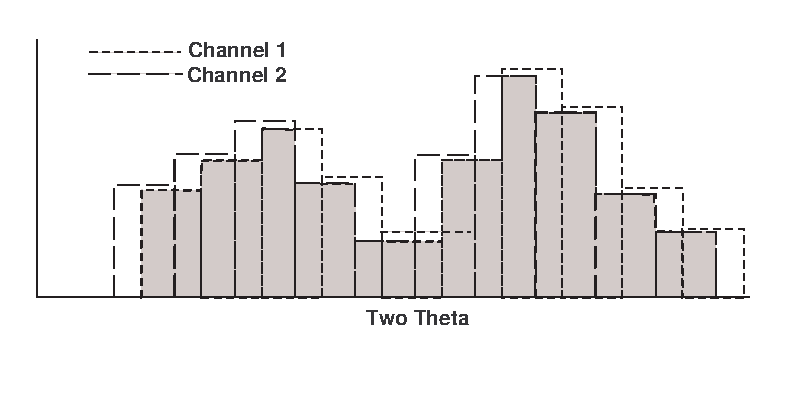
\includegraphics{offset.eps}
  \caption{Illustration of the overlap integral to be computed as a
  function of detector offset. The grey area represents the minimum of the 
  two patterns.}
  \label{fig:offset}
\end{figure}

Since the different channels might not be correctly scaled with respect to 
each other, the overlap will be normalised to the sum of the two individual 
channels over the given range.
The simplest way to do this seems to be to compute a correlation integral 
as a function of the detector offset. 
Assuming we have filled in the ascan array (from module rebin) with a set of 
counts and monitor counts we will just need a function to compute this 
integral for a given offset. 
The two theta bin centers and high and low limits will be given by the hard 
coded offsets in the program. 
If we subsequently decide these offsets are wrong then the scan will still 
need to be rebinned from the original data. 
This is a calculation which should only be done once in a while (the offsets 
are physically fixed on the instrument anyway).

\begin{flushleft} \small
\begin{minipage}{\linewidth}\label{scrap61}\raggedright\small
\NWtarget{nuweb57a}{} $\langle\,${\it crrfun}\nobreak\ {\footnotesize {57a}}$\,\rangle\equiv$
\vspace{-1ex}
\begin{list}{}{} \item
\mbox{}\verb@      real(kind=8) function crrfun(j)@\\
\mbox{}\verb@! Computes correlation function offset of n2 versus n1@\\
\mbox{}\verb@      use rebin ! contains ascan array and npts, ibin, tthhb etc@\\
\mbox{}\verb@      implicit none@\\
\mbox{}\verb@      integer(kind=4), intent(in) :: j@\\
\mbox{}\verb@      integer(kind=4) :: n1, n2@\\
\mbox{}\verb@      common/cfcom/ n1, n2@\\
\mbox{}\verb@      real(kind=8) :: s1, s2@\\
\mbox{}\verb@      integer(kind=4) :: n, i@\\
\mbox{}\verb@      crrfun=0.0d0; n=0@\\
\mbox{}\verb@      do i=1,npts@\\
\mbox{}\verb@        if((i+j).gt. 0 .and. (i+j).lt.npts)then@\\
\mbox{}\verb@        if(ascan(2*n1,i).gt.0.0d0 .and. ascan(2*n2,i+j).gt.0.0d0) then@\\
\mbox{}\verb@          n=n+1@\\
\mbox{}\verb@! signal in n1 and n2, n22@\\
\mbox{}\verb@          s1= ascan(2*n1-1,i)   /ascan(2*n1,i)@\\
\mbox{}\verb@          s2= ascan(2*n2-1,i+j) /ascan(2*n2,i+j)@\\
\mbox{}\verb@! crrfun is product of the two signals@\\
\mbox{}\verb@          crrfun=crrfun + s1*s2@\\
\mbox{}\verb@        endif; endif@\\
\mbox{}\verb@      enddo@\\
\mbox{}\verb@      crrfun=crrfun/real(n,8)@\\
\mbox{}\verb@      return@\\
\mbox{}\verb@      end function crrfun                                                    @{\NWsep}
\end{list}
\vspace{-1.5ex}
\footnotesize
\begin{list}{}{\setlength{\itemsep}{-\parsep}\setlength{\itemindent}{-\leftmargin}}
\item \NWtxtMacroRefIn\ \NWlink{nuweb57b}{57b}.

\item{}
\end{list}
\end{minipage}\vspace{4ex}
\end{flushleft}
As a test we should read a SPEC file in, rebinning it along the way and 
then compute the correlation function for each detector versus channels four.
Use a sharp dataset with good statistics and small binsize for this
to be effective. 

\begin{flushleft} \small\label{scrap62}\raggedright\small
\NWtarget{nuweb57b}{} \verb@"id31offsets.f90"@\nobreak\ {\footnotesize {57b}}$\equiv$
\vspace{-1ex}
\begin{list}{}{} \item
\mbox{}\verb@@\hbox{$\langle\,${\it specfiles}\nobreak\ {\footnotesize \NWlink{nuweb11a}{11a}}$\,\rangle$}\verb@@\\
\mbox{}\verb@@\hbox{$\langle\,${\it rebin}\nobreak\ {\footnotesize \NWlink{nuweb28}{28}}$\,\rangle$}\verb@ @\\
\mbox{}\verb@@\hbox{$\langle\,${\it summation}\nobreak\ {\footnotesize \NWlink{nuweb56}{56}}$\,\rangle$}\verb@@\\
\mbox{}\verb@@\hbox{$\langle\,${\it outputfiles}\nobreak\ {\footnotesize \NWlink{nuweb72}{72}}$\,\rangle$}\verb@@\\
\mbox{}\verb@@\hbox{$\langle\,${\it processscan}\nobreak\ {\footnotesize \NWlink{nuweb33}{33}}$\,\rangle$}\verb@@\\
\mbox{}\verb@@\hbox{$\langle\,${\it useroptions}\nobreak\ {\footnotesize \NWlink{nuweb87a}{87a}}$\,\rangle$}\verb@@\\
\mbox{}\verb@@\hbox{$\langle\,${\it tidyup}\nobreak\ {\footnotesize \NWlink{nuweb98}{98}}$\,\rangle$}\verb@@\\
\mbox{}\verb@@\hbox{$\langle\,${\it crrfun}\nobreak\ {\footnotesize \NWlink{nuweb57a}{57a}}$\,\rangle$}\verb@@\\
\mbox{}\verb@@\hbox{$\langle\,${\it helpmsg}\nobreak\ {\footnotesize \NWlink{nuweb87b}{87b}}$\,\rangle$}\verb@@\\
\mbox{}\verb@@\hbox{$\langle\,${\it id31offsetsmsg}\nobreak\ {\footnotesize \NWlink{nuweb59}{59}}$\,\rangle$}\verb@@\\
\mbox{}\verb@      program id31offsets@\\
\mbox{}\verb@      ! read and bin the scan(s)@\\
\mbox{}\verb@      ! calculate crrfun for each channel on a small tth range@\\
\mbox{}\verb@      use specfiles@\\
\mbox{}\verb@      use rebin@\\
\mbox{}\verb@!      use summation ! for user options - FIXME - module deps@\\
\mbox{}\verb@      use useroptions@\\
\mbox{}\verb@      use outputfiles@\\
\mbox{}\verb@      integer(kind=4) :: n1, n2@\\
\mbox{}\verb@      common/cfcom/ n1, n2@\\
\mbox{}\verb@      integer(kind=4)::i, j, ioffmin@\\
\mbox{}\verb@      real(kind=8) :: off, crr, crrmin, d1, d2, d21@\\
\mbox{}\verb@      real(kind=8) :: offm1, offp1, crrm1, crrp1@\\
\mbox{}\verb@      real start_time, end_time@\\
\mbox{}\verb@      real(kind=8) crrfun@\\
\mbox{}\verb@      external crrfun@\\
\mbox{}\verb@      call cpu_time(start_time)@\\
\mbox{}\verb@      call getcmdline                                 ! Get users options@\\
\mbox{}\verb@! fill out names of monitor, tth, first and last columns@\\
\mbox{}\verb@      if(snbl)then@\\
\mbox{}\verb@       MONITORCOL="Mon";FIRSTDET="Det1";LASTDET="Det6";TWOTTH="TwoTheta"@\\
\mbox{}\verb@       NCHANNEL=6@\\
\mbox{}\verb@      else@\\
\mbox{}\verb@       FIRSTDET="MA0";LASTDET="MA8";TWOTTH="2_theta"      @\\
\mbox{}\verb@       NCHANNEL=9@\\
\mbox{}\verb@      endif@\\
\mbox{}\verb@      call initialiserebin          ! Allocate space and check parameters@\\
\mbox{}\verb@      call getfile                                  ! Opens the spec file@\\
\mbox{}\verb@      call openlogfile    ! for counter details to be logged when binning@\\
\mbox{}\verb@      write(*,'(a,$)')'Binning scan '@\\
\mbox{}\verb@1     i=nextscan()                       ! Gets next scan to be processed@\\
\mbox{}\verb@      if(i.gt.0) then@\\
\mbox{}\verb@        call processscan(i)                       ! sums into ascan array@\\
\mbox{}\verb@        if(ispecerr.eq.-1)then@\\
\mbox{}\verb@           ispecerr=0@\\
\mbox{}\verb@           goto 1            ! next only if current was OK@\\
\mbox{}\verb@        endif   @\\
\mbox{}\verb@      endif@\\
\mbox{}\verb@      write(*,*) ! after non advancing io list of scans binned@\\
\mbox{}\verb@! Now for the actual channel calibration - data in ascan array of rebin@\\
\mbox{}\verb@      open(unit=20,file='offsets.out',status='UNKNOWN')@\\
\mbox{}\verb@      do i=1,9 ! all nine channels@\\
\mbox{}\verb@         if(logexdet(i).eq.1)then@\\
\mbox{}\verb@           write(*,1000)0.0d0,offset(i)  ! dont compute offset for channel@\\
\mbox{}\verb@           write(20,1000)0.0d0,offset(i)         @\\
\mbox{}\verb@          cycle@\\
\mbox{}\verb@         endif@\\
\mbox{}\verb@         if(i.eq.5) then@\\
\mbox{}\verb@           write(*,1000)0.0d0,offset(i)  ! compute the new offset for channel@\\
\mbox{}\verb@           write(20,1000)0.0d0,offset(i)@\\
\mbox{}\verb@           cycle@\\
\mbox{}\verb@         endif@\\
\mbox{}\verb@         n1=i; n2=5; crrmin=0.0d0@\\
\mbox{}\verb@         do j=-5,5,1@\\
\mbox{}\verb@           crr=crrfun(j)@\\
\mbox{}\verb@           if(crr.gt.crrmin)then; ioffmin=j; crrmin=crr; endif@\\
\mbox{}\verb@         enddo@\\
\mbox{}\verb@! Got the maximum of the function, now take the points on either side of it@\\
\mbox{}\verb@       offm1=real(ioffmin-1,8)*step; offp1=real(ioffmin+1,8)*step@\\
\mbox{}\verb@       off=real(ioffmin,8)*step; crr=crrfun(ioffmin)@\\
\mbox{}\verb@       crrm1=crrfun(ioffmin-1); crrp1=crrfun(ioffmin+1)@\\
\mbox{}\verb@! data three data points @\\
\mbox{}\verb@! (x0,y0), (x1,y1), (x2,y2) with xi != xj for i,j in {0,1,2}@\\
\mbox{}\verb@! set@\\
\mbox{}\verb@! d1=(y1-y0)/(x1-x0)@\\
\mbox{}\verb@! d2=(y2-y1)/(x2-x1)@\\
\mbox{}\verb@! d21=(d2-d1)/(x2-x0)@\\
\mbox{}\verb@! p2(x)  =  y0 + (x-x0)*(d1+(x-x1)*d21) @\\
\mbox{}\verb@!        =  x*d1 + x*(x-x1)*d21 - x0*x*d21  ! terms in x only     @\\
\mbox{}\verb@! dp2/dx =  0 at maximum (point of interest for us)@\\
\mbox{}\verb@!        =  d1 + 2 x d21 - x1 d21 - x0 d21 = 0@\\
\mbox{}\verb@!      x(at max) = ((x1 + x0)*d21 - d1 )/2*d21@\\
\mbox{}\verb@       d1=(crr-crrm1)/step; d2=(crrp1-crr)/step@\\
\mbox{}\verb@       d21=(d2-d1)/(2.0d0*step)@\\
\mbox{}\verb@       off = (d21*(offm1+off) - d1) / (2.0d0*d21)@\\
\mbox{}\verb@       offset(i)=offset(i)-off@\\
\mbox{}\verb@       write(*,1000)off,offset(i)  ! compute the new offset for channel@\\
\mbox{}\verb@       write(20,1000)off,offset(i)@\\
\mbox{}\verb@1000   format(10g20.10)@\\
\mbox{}\verb@      enddo@\\
\mbox{}\verb@      open(file='temp.new',status='UNKNOWN',form='FORMATTED',unit=18)@\\
\mbox{}\verb@      write(*,'(a)')'temp.new file to be created (copy over temp.res)'@\\
\mbox{}\verb@       if(snbl)then@\\
\mbox{}\verb@        do i=1,nchannel@\\
\mbox{}\verb@          write(*,1001)offset(i)-offset(1),mult(i),multerr(i),0.0d0@\\
\mbox{}\verb@          write(18,1001)offset(i)-offset(1),mult(i),multerr(i),0.0d0@\\
\mbox{}\verb@        enddo@\\
\mbox{}\verb@       else@\\
\mbox{}\verb@        do i=1,nchannel@\\
\mbox{}\verb@          write(*,1001)offset(i),mult(i),multerr(i),0.0d0@\\
\mbox{}\verb@          write(18,1001)offset(i),mult(i),multerr(i),0.0d0@\\
\mbox{}\verb@        enddo@\\
\mbox{}\verb@      endif@\\
\mbox{}\verb@1001 format(4(f11.8,','))@\\
\mbox{}\verb@      close(18)@\\
\mbox{}\verb@      call tidyup                                ! Frees allocated memory@\\
\mbox{}\verb@      call cpu_time(end_time)@\\
\mbox{}\verb@      write(*,'(a,f6.2,a)')'Time taken was ',end_time-start_time,'/s'      @\\
\mbox{}\verb@      end program id31offsets                                                @{\NWsep}
\end{list}
\vspace{-1.5ex}
\footnotesize
\begin{list}{}{\setlength{\itemsep}{-\parsep}\setlength{\itemindent}{-\leftmargin}}

\item{}
\end{list}
\vspace{4ex}
\end{flushleft}
\begin{flushleft} \small
\begin{minipage}{\linewidth}\label{scrap63}\raggedright\small
\NWtarget{nuweb59}{} $\langle\,${\it id31offsetsmsg}\nobreak\ {\footnotesize {59}}$\,\rangle\equiv$
\vspace{-1ex}
\begin{list}{}{} \item
\mbox{}\verb@1000  format('example: ',a,' file.dat 0.01 1 10    [snbl] '           &@\\
\mbox{}\verb@     &/'will process the scans 1 to 10  from file.dat with binsize 0.01'&@\\
\mbox{}\verb@     &/'to determine optimal detector offsets'                          &@\\
\mbox{}\verb@     &/'   snbl  if your data are in the Swiss Norwegian format'        &@\\
\mbox{}\verb@     &//'New values will be written to a temp.new file. You need a very'&@\\
\mbox{}\verb@     &/'good dataset to attempt this. A small stepsize is recommended.'/&@\\
\mbox{}\verb@     &/'Use the optional argument step=x.xxxx to force a small stepsize'&@\\
\mbox{}\verb@     &/'We recommend checking the results from this program.')@\\
\mbox{}\verb@     stop; end subroutine helpmsg                                            @{\NWsep}
\end{list}
\vspace{-1.5ex}
\footnotesize
\begin{list}{}{\setlength{\itemsep}{-\parsep}\setlength{\itemindent}{-\leftmargin}}
\item \NWtxtMacroRefIn\ \NWlink{nuweb57b}{57b}.

\item{}
\end{list}
\end{minipage}\vspace{4ex}
\end{flushleft}
\section{Writing output files}
Some bits and pieces for outputting the results of our efforts. 
We derive filenames from the variable \var{filnam} in the \mod{specfiles}
module. 
If it ends in a .dat extension then the extension is replaced with
something appropriate for the current output file, otherwise
the extension is appended.
Whether or not to write each kind of file will be determined by
the useroptions module.
A title, where it is needed can either come from the user options
module, or better something like the \#F line in the original SPEC
file.
Summary temperature information could also be included where allowed.

Variables to hold relevant parameters of interest are
\begin{flushleft} \small
\begin{minipage}{\linewidth}\label{scrap64}\raggedright\small
\NWtarget{nuweb60a}{} $\langle\,${\it outputfilesvars}\nobreak\ {\footnotesize {60a}}$\,\rangle\equiv$
\vspace{-1ex}
\begin{list}{}{} \item
\mbox{}\verb@       character(len=1024) :: outfile@\\
\mbox{}\verb@      integer(kind=4) :: ioutunit=11, ilow, ihigh, itot, logfile=21@\\
\mbox{}\verb@      logical :: gsas=.false. , spf=.false. , pds=.false., diag=.true.@\\
\mbox{}\verb@      logical :: epf=.false. , xye=.true.@\\
\mbox{}\verb@      character(len=1024) :: title                                           @{\NWsep}
\end{list}
\vspace{-1.5ex}
\footnotesize
\begin{list}{}{\setlength{\itemsep}{-\parsep}\setlength{\itemindent}{-\leftmargin}}
\item \NWtxtMacroRefIn\ \NWlink{nuweb72}{72}.

\item{}
\end{list}
\end{minipage}\vspace{4ex}
\end{flushleft}
\var{ilow} and \var{ihigh} are the first and last bins in the summed
array which are going to be output.

\subsection{Various file formats}

Most of this code is cut and pasted from Andy's epfout program, with 
adjustments to save reading in from an x,y,esd file.

\begin{flushleft} \small
\begin{minipage}{\linewidth}\label{scrap65}\raggedright\small
\NWtarget{nuweb60b}{} $\langle\,${\it scantitle}\nobreak\ {\footnotesize {60b}}$\,\rangle\equiv$
\vspace{-1ex}
\begin{list}{}{} \item
\mbox{}\verb@      if(is.gt.0)then@\\
\mbox{}\verb@       write(str,'(i10)')is; str=adjustl(str)@\\
\mbox{}\verb@       title=title(1:len_trim(title))//' Scan '//str(1:len_trim(str))@\\
\mbox{}\verb@      endif                                                                  @{\NWsep}
\end{list}
\vspace{-1.5ex}
\footnotesize
\begin{list}{}{\setlength{\itemsep}{-\parsep}\setlength{\itemindent}{-\leftmargin}}
\item \NWtxtMacroRefIn\ \NWlink{nuweb61}{61}\NWlink{nuweb63}{, 63}\NWlink{nuweb64a}{, 64a}.

\item{}
\end{list}
\end{minipage}\vspace{4ex}
\end{flushleft}
Firstly we attack the GSAS format. 
We will need the number of points being written, the minimum angle
and stepsize, both in centidegrees.
For now we will not allow data from negative angles or zero to be written
to the file (bitter experience suggests some old GSAS version didn't
appreciate these points).

\begin{flushleft} \small
\begin{minipage}{\linewidth}\label{scrap66}\raggedright\small
\NWtarget{nuweb61}{} $\langle\,${\it gsasout}\nobreak\ {\footnotesize {61}}$\,\rangle\equiv$
\vspace{-1ex}
\begin{list}{}{} \item
\mbox{}\verb@      subroutine gsasout(is)@\\
\mbox{}\verb@      use rebin ! ibin, bincen@\\
\mbox{}\verb@      use specfiles@\\
\mbox{}\verb@      use summation@\\
\mbox{}\verb@      integer(kind=4),intent(in)::is@\\
\mbox{}\verb@      integer(kind=4) :: low, ipts, nrec, i, k, n@\\
\mbox{}\verb@      real(kind=8), dimension(2,5) :: vals @\\
\mbox{}\verb@      real(kind=8) :: top ! for scaling to format@\\
\mbox{}\verb@      character(len=10) :: str@\\
\mbox{}\verb@      if(units.ne.'T')then@\\
\mbox{}\verb@        write(*,*)'Can only write GSAS format for two theta data'@\\
\mbox{}\verb@        stop@\\
\mbox{}\verb@      endif@\\
\mbox{}\verb@      call filext('.gsa',is)@\\
\mbox{}\verb@      open(file=outfile,unit=ioutunit,status='UNKNOWN')@\\
\mbox{}\verb@      write(title,1002)       specsfilename(1:len_trim(specsfilename)), &@\\
\mbox{}\verb@     & specsdate(1:len_trim(specsdate))@\\
\mbox{}\verb@1002  format(a,1X,a)      @\\
\mbox{}\verb@@\hbox{$\langle\,${\it scantitle}\nobreak\ {\footnotesize \NWlink{nuweb60b}{60b}}$\,\rangle$}\verb@    @\\
\mbox{}\verb@      write(ioutunit,'(a80)')title@\\
\mbox{}\verb@      write(ioutunit,1015)@\\
\mbox{}\verb@1015  format("Instrument parameter      id31.prm                  ",    &@\\
\mbox{}\verb@     & "                            ")@\\
\mbox{}\verb@      ilow=getfirstpoint(hist,2,npts,2)@\\
\mbox{}\verb@      ihigh=getlastpoint(hist,2,npts,2)@\\
\mbox{}\verb@      low=ibin(0.0d0)@\\
\mbox{}\verb@      if(low.gt.ilow) then ! the data goes below zero !@\\
\mbox{}\verb@       low=low+1           ! one point after zero@\\
\mbox{}\verb@      else@\\
\mbox{}\verb@       low=ilow         ! value from module@\\
\mbox{}\verb@      endif@\\
\mbox{}\verb@      ipts=ihigh-low    ! how many points for GSAS@\\
\mbox{}\verb@      nrec=(ipts-mod(ipts,5))/5  ! how many records@\\
\mbox{}\verb@      if(mod(ipts,5).ne.0)nrec=nrec+1@\\
\mbox{}\verb@      write(ioutunit,1000)ipts,nrec,bincen(low)*100.0d0,step*100.0d0@\\
\mbox{}\verb@!             1234567   +16     123456    20         123456789012 = 61(+19=80)@\\
\mbox{}\verb@1000  format('BANK 1 ',2(I7,1X),'CONST ',2(F9.3,1X),' 0.0 0.0 ESD'      &@\\
\mbox{}\verb@!        1234567890123456789@\\
\mbox{}\verb@     & ,'                   ')@\\
\mbox{}\verb@! scale factor to fit into F8.1 format? Max must be less than 999999@\\
\mbox{}\verb@      do i = low,ihigh@\\
\mbox{}\verb@        if(hist(1,i).gt.top)top=hist(1,i)@\\
\mbox{}\verb@      enddo@\\
\mbox{}\verb@      if (top.gt.999999.9d0)then@\\
\mbox{}\verb@        top=999999.9d0/top@\\
\mbox{}\verb@        write(*,'(a)')'Rescaled your data for GSAS to avoid overflows'@\\
\mbox{}\verb@        write(*,*)'   The data were multiplied by',top@\\
\mbox{}\verb@      else@\\
\mbox{}\verb@        top=1.0d0@\\
\mbox{}\verb@      endif@\\
\mbox{}\verb@      n = ipts-mod(ipts,5)@\\
\mbox{}\verb@      do i = low,n+low-1,5@\\
\mbox{}\verb@       do k=1,5@\\
\mbox{}\verb@         vals(1,k)=hist(1,k+i-1)*top@\\
\mbox{}\verb@         vals(2,k)=hist(2,k+i-1)*top@\\
\mbox{}\verb@         if (vals(2,k).lt.0.)then@\\
\mbox{}\verb@           vals(1,k)=0.0@\\
\mbox{}\verb@           vals(2,k)=999999.9@\\
\mbox{}\verb@         endif@\\
\mbox{}\verb@       enddo @\\
\mbox{}\verb@       write(ioutunit,'(10F8.1)')(vals(1,k),vals(2,k),k=1,5)@\\
\mbox{}\verb@      enddo@\\
\mbox{}\verb@      if(mod(ipts,5).ne.0) then@\\
\mbox{}\verb@        do k=low+n,ihigh@\\
\mbox{}\verb@          if (hist(2,k).gt.0.)then@\\
\mbox{}\verb@           vals(1,k+1-low-n)=hist(1,k)*top@\\
\mbox{}\verb@           vals(2,k+1-low-n)=hist(2,k)*top@\\
\mbox{}\verb@          else@\\
\mbox{}\verb@           vals(1,k+1-low-n)=0.@\\
\mbox{}\verb@           vals(1,k+1-low-n)=999999.9@\\
\mbox{}\verb@          endif@\\
\mbox{}\verb@        enddo@\\
\mbox{}\verb@        write(ioutunit,'(10F8.1)')(vals(1,k),vals(2,k),k=1,ihigh-low-n)@\\
\mbox{}\verb@      endif@\\
\mbox{}\verb@      close(ioutunit)@\\
\mbox{}\verb@      write(*,'(a)')'Wrote '//outfile(1:len_trim(outfile))@\\
\mbox{}\verb@      return@\\
\mbox{}\verb@      end subroutine gsasout                                                 @{\NWsep}
\end{list}
\vspace{-1.5ex}
\footnotesize
\begin{list}{}{\setlength{\itemsep}{-\parsep}\setlength{\itemindent}{-\leftmargin}}
\item \NWtxtMacroRefIn\ \NWlink{nuweb72}{72}.

\item{}
\end{list}
\end{minipage}\vspace{4ex}
\end{flushleft}
Now for something with the extension spf. 
\begin{flushleft} \small
\begin{minipage}{\linewidth}\label{scrap67}\raggedright\small
\NWtarget{nuweb63}{} $\langle\,${\it spfout}\nobreak\ {\footnotesize {63}}$\,\rangle\equiv$
\vspace{-1ex}
\begin{list}{}{} \item
\mbox{}\verb@      subroutine spfout(is)@\\
\mbox{}\verb@      use rebin@\\
\mbox{}\verb@      use summation@\\
\mbox{}\verb@      use specfiles@\\
\mbox{}\verb@      integer(kind=4),intent(in)::is@\\
\mbox{}\verb@      integer(kind=4)::low,ipts@\\
\mbox{}\verb@      character(len=18) :: time@\\
\mbox{}\verb@      character(len=10) :: str@\\
\mbox{}\verb@      integer(kind=4) :: n, i, k@\\
\mbox{}\verb@      character(len=3) :: months(12)@\\
\mbox{}\verb@      data months /'JAN','FEB','MAR','APR','MAY','JUN',                 &@\\
\mbox{}\verb@     &             'JUL','AUG','SEP','OCT','NOV','DEC'/@\\
\mbox{}\verb@      if(units.ne.'T')then@\\
\mbox{}\verb@        write(*,*)'Can only write SPF format for two theta data'@\\
\mbox{}\verb@        stop@\\
\mbox{}\verb@      endif@\\
\mbox{}\verb@      call filext('.spf',is)@\\
\mbox{}\verb@      open(file=outfile,unit=ioutunit,status='UNKNOWN')@\\
\mbox{}\verb@      ilow=getfirstpoint(hist,2,npts,2)@\\
\mbox{}\verb@      ihigh=getlastpoint(hist,2,npts,2)@\\
\mbox{}\verb@      low=ibin(0.0d0)@\\
\mbox{}\verb@      if(low.gt.ilow) then ! the data goes below zero !@\\
\mbox{}\verb@       low=low+1           ! one point after zero@\\
\mbox{}\verb@      else@\\
\mbox{}\verb@       low=ilow         ! value from module@\\
\mbox{}\verb@      endif@\\
\mbox{}\verb@      ipts=ihigh-low    ! how many points@\\
\mbox{}\verb@      n = ipts-mod(ipts,10) @\\
\mbox{}\verb@      write(title,1002)specsdate(1:len_trim(specsdate)),                &@\\
\mbox{}\verb@     &  specsfilename(1:len_trim(specsfilename))@\\
\mbox{}\verb@1002  format(a,1X,a)     @\\
\mbox{}\verb@@\hbox{$\langle\,${\it scantitle}\nobreak\ {\footnotesize \NWlink{nuweb60b}{60b}}$\,\rangle$}\verb@@\\
\mbox{}\verb@      write(ioutunit,'(a80)')title@\\
\mbox{}\verb@      write(ioutunit,2)ipts,bincen(low),bincen(ihigh),step@\\
\mbox{}\verb@ 2    format("       1       1       1"/1i8,"       1",                 &@\\
\mbox{}\verb@     & 3f10.3,"  0.000000  0.000000")@\\
\mbox{}\verb@!                               CCYYMMDD      HHMMSS.SSS@\\
\mbox{}\verb@       call date_and_time(date=time(1:8),time=time(9:18))@\\
\mbox{}\verb@! 123456789012345678@\\
\mbox{}\verb@! hh:mm:ss dd-mm-yy @\\
\mbox{}\verb@       read(time(5:6),'(i2)')i@\\
\mbox{}\verb@       time=time(9:10)//':'//time(11:12)//':'//time(13:14)//' '//       & @\\
\mbox{}\verb@     & time(7:8)//'-'//months(i)//'-'//time(3:4)@\\
\mbox{}\verb@       write(ioutunit,3)time(1:18)@\\
\mbox{}\verb@ 3     format("  100000.0       0.0     ",1a18,                         &@\\
\mbox{}\verb@     & "      0      0 SYNCHROTRON  ID31 ESRF"/8("     0.000"))@\\
\mbox{}\verb@       do i = low,n+low-1,10@\\
\mbox{}\verb@       write(ioutunit,4)bincen(i),(nint(hist(1,k)),k=i,i+9)@\\
\mbox{}\verb@       write(ioutunit,5)(hist(2,k),k=i,i+9)@\\
\mbox{}\verb@ 4     format(1f8.3,10i7)@\\
\mbox{}\verb@ 5     format(8x,10f7.2)@\\
\mbox{}\verb@       enddo@\\
\mbox{}\verb@       if(mod(ipts,10).ne.0)then @\\
\mbox{}\verb@       write(ioutunit,4)bincen(n+low),(nint(hist(1,k)),k=n+low,ipts)@\\
\mbox{}\verb@       write(ioutunit,5)(hist(2,k),k=n+low,ipts)@\\
\mbox{}\verb@       endif@\\
\mbox{}\verb@       write(ioutunit,6)@\\
\mbox{}\verb@ 6     format('       0 HKL reflection(s)'/                             &@\\
\mbox{}\verb@      & '       0 excluded region(s)')                                  @\\
\mbox{}\verb@       close(ioutunit)@\\
\mbox{}\verb@       write(*,'(a)')'Wrote '//outfile(1:len_trim(outfile))@\\
\mbox{}\verb@       end subroutine spfout                                                 @{\NWsep}
\end{list}
\vspace{-1.5ex}
\footnotesize
\begin{list}{}{\setlength{\itemsep}{-\parsep}\setlength{\itemindent}{-\leftmargin}}
\item \NWtxtMacroRefIn\ \NWlink{nuweb72}{72}.

\item{}
\end{list}
\end{minipage}\vspace{4ex}
\end{flushleft}
Winmprof likes to have files in something called pds format.
Here's something to produce that format.

\begin{flushleft} \small
\begin{minipage}{\linewidth}\label{scrap68}\raggedright\small
\NWtarget{nuweb64a}{} $\langle\,${\it pdsout}\nobreak\ {\footnotesize {64a}}$\,\rangle\equiv$
\vspace{-1ex}
\begin{list}{}{} \item
\mbox{}\verb@       subroutine pdsout(is)@\\
\mbox{}\verb@      use rebin@\\
\mbox{}\verb@      use summation@\\
\mbox{}\verb@      use specfiles@\\
\mbox{}\verb@      integer(kind=4),intent(in)::is@\\
\mbox{}\verb@      integer (kind=4) :: low, ipts, i, k, n@\\
\mbox{}\verb@      character(len=10):: str@\\
\mbox{}\verb@      if(units.ne.'T')then@\\
\mbox{}\verb@        write(*,*)'Can only write PDS format for two theta data'@\\
\mbox{}\verb@        stop@\\
\mbox{}\verb@      endif@\\
\mbox{}\verb@      call filext('.pds',is)@\\
\mbox{}\verb@      open(file=outfile,unit=ioutunit,status='UNKNOWN')    @\\
\mbox{}\verb@      write(title,1002)specsdate(1:len_trim(specsdate)),                &@\\
\mbox{}\verb@     &  specsfilename(1:len_trim(specsfilename))@\\
\mbox{}\verb@1002  format(a,1X,a)      @\\
\mbox{}\verb@@\hbox{$\langle\,${\it scantitle}\nobreak\ {\footnotesize \NWlink{nuweb60b}{60b}}$\,\rangle$}\verb@@\\
\mbox{}\verb@      write(ioutunit,'(1a80)')title      @\\
\mbox{}\verb@      write(ioutunit,7)@\\
\mbox{}\verb@      ilow=getfirstpoint(hist,2,npts,2)@\\
\mbox{}\verb@      ihigh=getlastpoint(hist,2,npts,2)@\\
\mbox{}\verb@      low=ibin(0.0d0)@\\
\mbox{}\verb@      if(low.gt.ilow) then ! the data goes below zero !@\\
\mbox{}\verb@       low=low+1           ! one point after zero@\\
\mbox{}\verb@      else@\\
\mbox{}\verb@       low=ilow         ! value from module@\\
\mbox{}\verb@      endif@\\
\mbox{}\verb@      ipts=ihigh-low@\\
\mbox{}\verb@7     format("   Start     Step      End     Monitor")@\\
\mbox{}\verb@      write(ioutunit,8)bincen(low),step,bincen(ihigh)@\\
\mbox{}\verb@8     format(3f9.3,'    10000')@\\
\mbox{}\verb@      n = ipts-mod(ipts,10) @\\
\mbox{}\verb@      do 800 i = low,n+low-1,10@\\
\mbox{}\verb@        write(ioutunit,9)(hist(2,k),k=i,i+9)@\\
\mbox{}\verb@        write(ioutunit,10)(nint(hist(1,k)),k=i,i+9)@\\
\mbox{}\verb@9     format(10f8.4)@\\
\mbox{}\verb@10    format(10i8)@\\
\mbox{}\verb@800   continue@\\
\mbox{}\verb@      if(mod(ipts,10).ne.0)then@\\
\mbox{}\verb@       write(ioutunit,9)(hist(2,k),k=n+1,ipts)@\\
\mbox{}\verb@       write(ioutunit,10)(nint(hist(1,k)),k=n+1,ipts)@\\
\mbox{}\verb@      endif@\\
\mbox{}\verb@      write(ioutunit,11)@\\
\mbox{}\verb@11    format('   -1000'/'  -10000')@\\
\mbox{}\verb@      close(ioutunit)@\\
\mbox{}\verb@      write(*,'(a)')'Wrote '//outfile(1:len_trim(outfile))@\\
\mbox{}\verb@      return; end subroutine pdsout                                         @{\NWsep}
\end{list}
\vspace{-1.5ex}
\footnotesize
\begin{list}{}{\setlength{\itemsep}{-\parsep}\setlength{\itemindent}{-\leftmargin}}
\item \NWtxtMacroRefIn\ \NWlink{nuweb72}{72}.

\item{}
\end{list}
\end{minipage}\vspace{4ex}
\end{flushleft}
\subsection{Diagnostic plots}

When there is some kind of problem with the binning we will need to 
write out a diagnostic file showing what each of the separate
channels has recorded.

\begin{flushleft} \small\label{scrap69}\raggedright\small
\NWtarget{nuweb64b}{} $\langle\,${\it outputdiagnostic}\nobreak\ {\footnotesize {64b}}$\,\rangle\equiv$
\vspace{-1ex}
\begin{list}{}{} \item
\mbox{}\verb@      subroutine outputdiagnostic(wd)@\\
\mbox{}\verb@      use rebin ! ascan@\\
\mbox{}\verb@      use summation@\\
\mbox{}\verb@      real(kind=8),intent(in)::wd@\\
\mbox{}\verb@      integer(kind=4) :: i, ihigh, ilow, j@\\
\mbox{}\verb@      real(kind=8) :: y, ey2, wd2@\\
\mbox{}\verb@! write a file in plotmtv format with the 9 channels and sum@\\
\mbox{}\verb@      open(unit=ioutunit,file='diag.mtv',status='UNKNOWN',              &@\\
\mbox{}\verb@     & form='FORMATTED', access='SEQUENTIAL',iostat=i) @\\
\mbox{}\verb@      if(i.ne.0)then@\\
\mbox{}\verb@       write(*,'(a)')'error opening diagnostic file'@\\
\mbox{}\verb@      endif@\\
\mbox{}\verb@      write(ioutunit,'(a)')'$ DATA = CURVE2D'@\\
\mbox{}\verb@      write(ioutunit,'(a)')'% xlabel = "Two Theta"'@\\
\mbox{}\verb@      write(ioutunit,'(a)')'% ylabel = "Cts/Monitor"'@\\
\mbox{}\verb@      write(ioutunit,'(a)')'% toplabel= "Diagnostic plot"'@\\
\mbox{}\verb@      do j=1,nchannel@\\
\mbox{}\verb@! j-1 to fix the zeroth channel being first@\\
\mbox{}\verb@       write(ioutunit,'(a,i1,a)')'% linelabel = " MA',j-1,' "'      @\\
\mbox{}\verb@       write(ioutunit,'(a,i2)')'% linecolor = ',j      @\\
\mbox{}\verb@       write(ioutunit,'(a)')'% linetype=1 markertype=0'      @\\
\mbox{}\verb@       ilow=getfirstpoint(ascan,2*nchannel,npts,2*j)@\\
\mbox{}\verb@       ihigh=getlastpoint(ascan,2*nchannel,npts,2*j)@\\
\mbox{}\verb@       do i=ilow,ihigh@\\
\mbox{}\verb@        if(ascan(2*j,i).gt.1.0d0)                                       &@\\
\mbox{}\verb@        write(ioutunit,'(2F15.8)')bincen(i),                            &@\\
\mbox{}\verb@     & ascan(2*j-1,i)/ascan(2*j,i)/mult(j)@\\
\mbox{}\verb@       enddo@\\
\mbox{}\verb@       write(ioutunit,*)@\\
\mbox{}\verb@      enddo@\\
\mbox{}\verb@      write(ioutunit,'(a,i2,a)')'% linelabel = "Total"'      @\\
\mbox{}\verb@      write(ioutunit,'(a,i2)')'% linecolor = ',nchannel+1      @\\
\mbox{}\verb@      write(ioutunit,'(a)')'% linetype=1 markertype=0'@\\
\mbox{}\verb@      ilow=getfirstpoint(hist,2,npts,2)@\\
\mbox{}\verb@      ihigh=getlastpoint(hist,2,npts,2)@\\
\mbox{}\verb@      do i=ilow,ihigh@\\
\mbox{}\verb@        write(ioutunit,'(2F15.8)')bincen(i),hist(1,i)@\\
\mbox{}\verb@      enddo@\\
\mbox{}\verb@      write(ioutunit,*)@\\
\mbox{}\verb@      write(ioutunit,'(a,i2,a)')'% linelabel = "outliers"'      @\\
\mbox{}\verb@      write(ioutunit,'(a,i2)')'% markercolor = ',nchannel+2      @\\
\mbox{}\verb@      write(ioutunit,'(a)')'% linetype=0 markertype=2'@\\
\mbox{}\verb@      do i=ilow,ihigh@\\
\mbox{}\verb@        if(ctchan(i).ge.2)then@\\
\mbox{}\verb@        do j=1,nchannel@\\
\mbox{}\verb@          if(ascan(2*j,i).gt.1.0d0)then@\\
\mbox{}\verb@@\hbox{$\langle\,${\it getwd2}\nobreak\ {\footnotesize \NWlink{nuweb49}{49}}$\,\rangle$}\verb@@\\
\mbox{}\verb@            if(wd2.gt.wd)write(ioutunit,'(2F15.8)')bincen(i),y@\\
\mbox{}\verb@          endif@\\
\mbox{}\verb@        enddo@\\
\mbox{}\verb@        endif@\\
\mbox{}\verb@      enddo@\\
\mbox{}\verb@      write(ioutunit,*)@\\
\mbox{}\verb@      write(ioutunit,'(a)')'$ END'@\\
\mbox{}\verb@      write(*,'(a,G12.5)')'Wrote diag.mtv file, outliers at ',sqrt(wd)@\\
\mbox{}\verb@      close(ioutunit)@\\
\mbox{}\verb@      return@\\
\mbox{}\verb@      end subroutine outputdiagnostic                                        @{\NWsep}
\end{list}
\vspace{-1.5ex}
\footnotesize
\begin{list}{}{\setlength{\itemsep}{-\parsep}\setlength{\itemindent}{-\leftmargin}}
\item \NWtxtMacroRefIn\ \NWlink{nuweb72}{72}.

\item{}
\end{list}
\vspace{4ex}
\end{flushleft}
The w32 version of this program writes out the diagnostic plot file in a format
suiatable for the presto plotting program (a windows port of xmgr/grace).
\begin{flushleft} \small\label{scrap70}\raggedright\small
\NWtarget{nuweb66}{} $\langle\,${\it outputdiagnosticw32}\nobreak\ {\footnotesize {66}}$\,\rangle\equiv$
\vspace{-1ex}
\begin{list}{}{} \item
\mbox{}\verb@      subroutine outputdiagnosticw32(wd)@\\
\mbox{}\verb@      use rebin ! ascan@\\
\mbox{}\verb@      use summation@\\
\mbox{}\verb@      real(kind=8),intent(in)::wd@\\
\mbox{}\verb@      integer(kind=4) :: i, j, k@\\
\mbox{}\verb@      real(kind=8) :: y, ey2, wd2@\\
\mbox{}\verb@! write a file in plotmtv format with the 9 channels and sum@\\
\mbox{}\verb@      open(unit=ioutunit,file='diag.mtv',status='UNKNOWN',              &@\\
\mbox{}\verb@     & form='FORMATTED', access='SEQUENTIAL',iostat=i) @\\
\mbox{}\verb@      if(i.ne.0)then@\\
\mbox{}\verb@       write(*,'(a)') 'error opening diagnostic file'@\\
\mbox{}\verb@       stop@\\
\mbox{}\verb@      endif@\\
\mbox{}\verb@      write(ioutunit,'(a)')'#@{\tt @}\verb@set[0].point.style none'@\\
\mbox{}\verb@      write(ioutunit,'(a)')'#@{\tt @}\verb@set[1].point.style none'@\\
\mbox{}\verb@      write(ioutunit,'(a)')'#@{\tt @}\verb@set[2].point.style none'@\\
\mbox{}\verb@      write(ioutunit,'(a)')'#@{\tt @}\verb@set[3].point.style none'@\\
\mbox{}\verb@      write(ioutunit,'(a)')'#@{\tt @}\verb@set[4].point.style none'@\\
\mbox{}\verb@      write(ioutunit,'(a)')'#@{\tt @}\verb@set[5].point.style none'@\\
\mbox{}\verb@      write(ioutunit,'(a)')'#@{\tt @}\verb@set[6].point.style none'@\\
\mbox{}\verb@      write(ioutunit,'(a)')'#@{\tt @}\verb@set[7].point.style none'@\\
\mbox{}\verb@      write(ioutunit,'(a)')'#@{\tt @}\verb@set[8].point.style none'@\\
\mbox{}\verb@      write(ioutunit,'(a)')'#@{\tt @}\verb@set[9].point.style none'@\\
\mbox{}\verb@      write(ioutunit,'(a)')'#@{\tt @}\verb@set[10].point.style circle'@\\
\mbox{}\verb@      write(ioutunit,'(a)')'#@{\tt @}\verb@set[0].line.style solid'@\\
\mbox{}\verb@      write(ioutunit,'(a)')'#@{\tt @}\verb@set[1].line.style solid'@\\
\mbox{}\verb@      write(ioutunit,'(a)')'#@{\tt @}\verb@set[2].line.style solid'@\\
\mbox{}\verb@      write(ioutunit,'(a)')'#@{\tt @}\verb@set[3].line.style solid'@\\
\mbox{}\verb@      write(ioutunit,'(a)')'#@{\tt @}\verb@set[4].line.style solid'@\\
\mbox{}\verb@      write(ioutunit,'(a)')'#@{\tt @}\verb@set[5].line.style solid'@\\
\mbox{}\verb@      write(ioutunit,'(a)')'#@{\tt @}\verb@set[6].line.style solid'@\\
\mbox{}\verb@      write(ioutunit,'(a)')'#@{\tt @}\verb@set[7].line.style solid'@\\
\mbox{}\verb@      write(ioutunit,'(a)')'#@{\tt @}\verb@set[8].line.style solid'@\\
\mbox{}\verb@      write(ioutunit,'(a)')'#@{\tt @}\verb@set[9].line.style solid'@\\
\mbox{}\verb@      write(ioutunit,'(a)')'#@{\tt @}\verb@set[10].line.style none'@\\
\mbox{}\verb@      write(ioutunit,'(a)')'#@{\tt @}\verb@set[0].line.color custom 255 0   0'@\\
\mbox{}\verb@      write(ioutunit,'(a)')'#@{\tt @}\verb@set[1].line.color custom 215 30  0'@\\
\mbox{}\verb@      write(ioutunit,'(a)')'#@{\tt @}\verb@set[2].line.color custom 180 60  0'@\\
\mbox{}\verb@      write(ioutunit,'(a)')'#@{\tt @}\verb@set[3].line.color custom 150 90  0'@\\
\mbox{}\verb@      write(ioutunit,'(a)')'#@{\tt @}\verb@set[4].line.color custom 120 120 0'@\\
\mbox{}\verb@      write(ioutunit,'(a)')'#@{\tt @}\verb@set[5].line.color custom 90  150 0'@\\
\mbox{}\verb@      write(ioutunit,'(a)')'#@{\tt @}\verb@set[6].line.color custom 60  180 0'@\\
\mbox{}\verb@      write(ioutunit,'(a)')'#@{\tt @}\verb@set[7].line.color custom 30  215 0'@\\
\mbox{}\verb@      write(ioutunit,'(a)')'#@{\tt @}\verb@set[8].line.color custom 0   25  0'@\\
\mbox{}\verb@      write(ioutunit,'(a)')'#@{\tt @}\verb@set[9].line.color custom 0   0   0'@\\
\mbox{}\verb@      write(ioutunit,'(a)')'#@{\tt @}\verb@set[10].point.color custom 0 0 0'@\\
\mbox{}\verb@      do i=1,npts@\\
\mbox{}\verb@      if(ctchan(i).lt.1)cycle@\\
\mbox{}\verb@      write(ioutunit,'(11F15.8)',advance='no')bincen(i),                &@\\
\mbox{}\verb@     &(ascan(2*j-1,i)/(1.0d0+ascan(2*j,i)*mult(j)), j=1,nchannel),      &@\\
\mbox{}\verb@     &hist(1,i)@\\
\mbox{}\verb@      k=0@\\
\mbox{}\verb@      if(ctchan(i).ge.2)then  @\\
\mbox{}\verb@        do j=1,nchannel@\\
\mbox{}\verb@          if(ascan(2*j,i).gt.1.0d0)then@\\
\mbox{}\verb@@\hbox{$\langle\,${\it getwd2}\nobreak\ {\footnotesize \NWlink{nuweb49}{49}}$\,\rangle$}\verb@@\\
\mbox{}\verb@            if(wd2.gt.wd .and. k.eq.0)then@\\
\mbox{}\verb@              write(ioutunit,'(F15.8)')                                 &@\\
\mbox{}\verb@     &            ascan(2*j-1,i)/(ascan(2*j,i)*mult(j))   @\\
\mbox{}\verb@              k=1@\\
\mbox{}\verb@            endif@\\
\mbox{}\verb@          endif@\\
\mbox{}\verb@        enddo@\\
\mbox{}\verb@      endif@\\
\mbox{}\verb@      if(k.eq.0)write(ioutunit,'(F15.8)')-0.001d0@\\
\mbox{}\verb@      enddo@\\
\mbox{}\verb@      write(ioutunit,*)@\\
\mbox{}\verb@      write(*,'(a,G12.5)')'Wrote diag.mtv file, outliers at ',sqrt(wd)@\\
\mbox{}\verb@      close(ioutunit)@\\
\mbox{}\verb@      return; end subroutine outputdiagnosticw32                             @{\NWsep}
\end{list}
\vspace{-1.5ex}
\footnotesize
\begin{list}{}{\setlength{\itemsep}{-\parsep}\setlength{\itemindent}{-\leftmargin}}
\item \NWtxtMacroRefIn\ \NWlink{nuweb72}{72}.

\item{}
\end{list}
\vspace{4ex}
\end{flushleft}
\begin{flushleft} \small
\begin{minipage}{\linewidth}\label{scrap71}\raggedright\small
\NWtarget{nuweb67}{} $\langle\,${\it dumpscan}\nobreak\ {\footnotesize {67}}$\,\rangle\equiv$
\vspace{-1ex}
\begin{list}{}{} \item
\mbox{}\verb@      subroutine dumpscan(is)@\\
\mbox{}\verb@      use rebin@\\
\mbox{}\verb@      integer(kind=4) :: i, j@\\
\mbox{}\verb@      integer(kind=4),intent(in)::is@\\
\mbox{}\verb@      real(kind=8),dimension(9) :: sig@\\
\mbox{}\verb@      call filext('.dum',is)@\\
\mbox{}\verb@      open(unit=ioutunit,file=outfile,status='UNKNOWN',                 &@\\
\mbox{}\verb@     & form='FORMATTED',access='SEQUENTIAL',iostat=i)@\\
\mbox{}\verb@      if(i.ne.0) stop 'error opening output file'@\\
\mbox{}\verb@      do i=1,npts@\\
\mbox{}\verb@        do j=1,9@\\
\mbox{}\verb@          if(ascan(2*j,i).gt.0)then@\\
\mbox{}\verb@            sig(j)=ascan(2*j-1,i)/ascan(2*j,i)@\\
\mbox{}\verb@          else@\\
\mbox{}\verb@             sig(j)=0.0@\\
\mbox{}\verb@          endif@\\
\mbox{}\verb@        enddo@\\
\mbox{}\verb@        write(ioutunit,'(10(F12.8,1X))')bincen(i),(sig(j),j=1,9)@\\
\mbox{}\verb@      enddo@\\
\mbox{}\verb@      close(ioutunit)@\\
\mbox{}\verb@      return  @\\
\mbox{}\verb@      end subroutine dumpscan                                                @{\NWsep}
\end{list}
\vspace{-1.5ex}
\footnotesize
\begin{list}{}{\setlength{\itemsep}{-\parsep}\setlength{\itemindent}{-\leftmargin}}
\item \NWtxtMacroRefIn\ \NWlink{nuweb72}{72}.

\item{}
\end{list}
\end{minipage}\vspace{4ex}
\end{flushleft}
We should have an "undumpscan" routine which can take up where
dumpscan has left off. It just needs to include some additional information
in the dumped out format. This was only ever included for debugging and
on line viewing of detector channels - so perhaps a bit pointless.
FIXME - range of scan to dump.

\subsection{epf and inp formats}

\begin{flushleft} \small
\begin{minipage}{\linewidth}\label{scrap72}\raggedright\small
\NWtarget{nuweb68a}{} $\langle\,${\it outputepf}\nobreak\ {\footnotesize {68a}}$\,\rangle\equiv$
\vspace{-1ex}
\begin{list}{}{} \item
\mbox{}\verb@      subroutine epfout(n)@\\
\mbox{}\verb@      use rebin@\\
\mbox{}\verb@      use summation@\\
\mbox{}\verb@      integer(kind=4) :: i, ilow, ihigh, n@\\
\mbox{}\verb@      call filext('.epf',n) ! epfs never refer to a scan, always a sum@\\
\mbox{}\verb@      open(unit=ioutunit,status='UNKNOWN',file=outfile)@\\
\mbox{}\verb@      ilow=getfirstpoint(hist,2,npts,2)@\\
\mbox{}\verb@      ihigh=getlastpoint(hist,2,npts,2)@\\
\mbox{}\verb@      if(ilow.eq.-1 .or. ihigh.eq.-1)then@\\
\mbox{}\verb@       ! No points with valid data found !@\\
\mbox{}\verb@       return@\\
\mbox{}\verb@      endif@\\
\mbox{}\verb@      do i=ilow,ihigh     @\\
\mbox{}\verb@        write(ioutunit,*)bincen(i),hist(1,i),hist(2,i)@\\
\mbox{}\verb@      enddo@\\
\mbox{}\verb@      close(ioutunit)@\\
\mbox{}\verb@      write(*,'(a)')'Wrote '//outfile(1:len_trim(outfile))      @\\
\mbox{}\verb@      return@\\
\mbox{}\verb@      end subroutine epfout                                               @{\NWsep}
\end{list}
\vspace{-1.5ex}
\footnotesize
\begin{list}{}{\setlength{\itemsep}{-\parsep}\setlength{\itemindent}{-\leftmargin}}
\item \NWtxtMacroRefIn\ \NWlink{nuweb72}{72}.

\item{}
\end{list}
\end{minipage}\vspace{4ex}
\end{flushleft}
\begin{flushleft} \small
\begin{minipage}{\linewidth}\label{scrap73}\raggedright\small
\NWtarget{nuweb68b}{} $\langle\,${\it outputxye}\nobreak\ {\footnotesize {68b}}$\,\rangle\equiv$
\vspace{-1ex}
\begin{list}{}{} \item
\mbox{}\verb@      subroutine xyeout(n)@\\
\mbox{}\verb@      use rebin@\\
\mbox{}\verb@      use summation@\\
\mbox{}\verb@      integer(kind=4) :: i, ilow, ihigh, n@\\
\mbox{}\verb@      character(len=4) :: extn@\\
\mbox{}\verb@      if(units .eq. 'T') extn = '.xye'@\\
\mbox{}\verb@      if(units .eq. 'Q') extn = '.qye'@\\
\mbox{}\verb@      if(units .eq. 'R') extn = '.q2'@\\
\mbox{}\verb@      call filext(extn,n) ! epfs never refer to a scan, always a sum@\\
\mbox{}\verb@      open(unit=ioutunit,status='UNKNOWN',file=outfile)@\\
\mbox{}\verb@      ilow=getfirstpoint(hist,2,npts,2)@\\
\mbox{}\verb@      ihigh=getlastpoint(hist,2,npts,2)@\\
\mbox{}\verb@      if(ilow.eq.-1 .or. ihigh.eq.-1)then@\\
\mbox{}\verb@       ! No points with valid data found !@\\
\mbox{}\verb@       return@\\
\mbox{}\verb@      endif@\\
\mbox{}\verb@      do i=ilow,ihigh     @\\
\mbox{}\verb@        write(ioutunit,'(F12.6,2(1X,G14.8))')bincen(i),hist(1,i),hist(2,i)@\\
\mbox{}\verb@      enddo@\\
\mbox{}\verb@      close(ioutunit)@\\
\mbox{}\verb@      write(*,'(a)')'Wrote '//outfile(1:len_trim(outfile))      @\\
\mbox{}\verb@      return@\\
\mbox{}\verb@      end subroutine xyeout                                               @{\NWsep}
\end{list}
\vspace{-1.5ex}
\footnotesize
\begin{list}{}{\setlength{\itemsep}{-\parsep}\setlength{\itemindent}{-\leftmargin}}
\item \NWtxtMacroRefIn\ \NWlink{nuweb72}{72}.

\item{}
\end{list}
\end{minipage}\vspace{4ex}
\end{flushleft}
\begin{flushleft} \small
\begin{minipage}{\linewidth}\label{scrap74}\raggedright\small
\NWtarget{nuweb69a}{} $\langle\,${\it outputinp}\nobreak\ {\footnotesize {69a}}$\,\rangle\equiv$
\vspace{-1ex}
\begin{list}{}{} \item
\mbox{}\verb@      subroutine outputinp(n)@\\
\mbox{}\verb@      use rebin@\\
\mbox{}\verb@      use summation@\\
\mbox{}\verb@      integer(kind=4),intent(in)::n@\\
\mbox{}\verb@      integer(kind=4) :: i, ilow, ihigh@\\
\mbox{}\verb@      character(len=15):: string@\\
\mbox{}\verb@      write(string,'(i10)')n@\\
\mbox{}\verb@      string=adjustl(string)@\\
\mbox{}\verb@      if(units.eq.'T') string=string(1:len_trim(string))//'.inp'@\\
\mbox{}\verb@      if(units.eq.'Q') string=string(1:len_trim(string))//'.inq'@\\
\mbox{}\verb@      if(units.eq.'R') string=string(1:len_trim(string))//'.inq2'@\\
\mbox{}\verb@!      write(*,*)'String was ',string@\\
\mbox{}\verb@      open(unit=ioutunit,status='UNKNOWN',file=string)@\\
\mbox{}\verb@      ilow=getfirstpoint(hist,2,npts,2)@\\
\mbox{}\verb@      ihigh=getlastpoint(hist,2,npts,2)@\\
\mbox{}\verb@      if(ilow.eq.-1 .or. ihigh.eq.-1)then@\\
\mbox{}\verb@       ! No points with valid data found !@\\
\mbox{}\verb@       return@\\
\mbox{}\verb@      endif@\\
\mbox{}\verb@      do i=ilow,ihigh     @\\
\mbox{}\verb@        write(ioutunit,*)bincen(i),hist(1,i),hist(2,i)@\\
\mbox{}\verb@      enddo@\\
\mbox{}\verb@      close(ioutunit)@\\
\mbox{}\verb@      write(*,'(a)')'Wrote '//string(1:len_trim(string)) @\\
\mbox{}\verb@      return@\\
\mbox{}\verb@      end subroutine outputinp                                               @{\NWsep}
\end{list}
\vspace{-1.5ex}
\footnotesize
\begin{list}{}{\setlength{\itemsep}{-\parsep}\setlength{\itemindent}{-\leftmargin}}
\item \NWtxtMacroRefIn\ \NWlink{nuweb72}{72}.

\item{}
\end{list}
\end{minipage}\vspace{4ex}
\end{flushleft}
\subsection{Logfiles}

When running through the binning program there is a fair bit of information
which we might want to preserve - the kind of thing which belongs in a 
lab notebook. 
Much of this will flash past on the screen before anyone has a chance to see
it, so the plan is to write things like motor positions, dates, temperatures
and so on to a logfile for the particular binning run. 

We will need (at least) three routines - one to start a log, another to
write to it and finally a close at the end. 
The closing will be done by the general \code{tidyup} routine, so in fact
we only need to provide the first two.

\begin{flushleft} \small
\begin{minipage}{\linewidth}\label{scrap75}\raggedright\small
\NWtarget{nuweb69b}{} $\langle\,${\it openlogfile}\nobreak\ {\footnotesize {69b}}$\,\rangle\equiv$
\vspace{-1ex}
\begin{list}{}{} \item
\mbox{}\verb@      subroutine openlogfile@\\
\mbox{}\verb@      integer(kind=4) :: i@\\
\mbox{}\verb@      call filext('.log',0) ! logfiles for all scans, not one each@\\
\mbox{}\verb@      open(unit=logfile,file=outfile,status='UNKNOWN',                  &@\\
\mbox{}\verb@     & form='FORMATTED',access='SEQUENTIAL',iostat=i)@\\
\mbox{}\verb@      if(i.ne.0)stop 'could not open logfile'@\\
\mbox{}\verb@      return; end subroutine openlogfile                                     @{\NWsep}
\end{list}
\vspace{-1.5ex}
\footnotesize
\begin{list}{}{\setlength{\itemsep}{-\parsep}\setlength{\itemindent}{-\leftmargin}}
\item \NWtxtMacroRefIn\ \NWlink{nuweb72}{72}.

\item{}
\end{list}
\end{minipage}\vspace{4ex}
\end{flushleft}
Since the outputfiles module uses the various other modules, this routine
cannot be available to any routine which is contained in another module.
Only main programs or the processscan stuff can access the log file. 
This is a sort of intentional design decision... the subroutines which are
in modules aren't meant to be doing any user type io, even if they currently
are.

\begin{flushleft} \small
\begin{minipage}{\linewidth}\label{scrap76}\raggedright\small
\NWtarget{nuweb70a}{} $\langle\,${\it wlogfile}\nobreak\ {\footnotesize {70a}}$\,\rangle\equiv$
\vspace{-1ex}
\begin{list}{}{} \item
\mbox{}\verb@      subroutine wlogfile(s)@\\
\mbox{}\verb@      character(len=*) :: s@\\
\mbox{}\verb@      write(logfile,'(a)')s@\\
\mbox{}\verb@      return; end subroutine wlogfile                                        @{\NWsep}
\end{list}
\vspace{-1.5ex}
\footnotesize
\begin{list}{}{\setlength{\itemsep}{-\parsep}\setlength{\itemindent}{-\leftmargin}}
\item \NWtxtMacroRefIn\ \NWlink{nuweb72}{72}.

\item{}
\end{list}
\end{minipage}\vspace{4ex}
\end{flushleft}
\subsection{Utils}

\begin{flushleft} \small
\begin{minipage}{\linewidth}\label{scrap77}\raggedright\small
\NWtarget{nuweb70b}{} $\langle\,${\it filext}\nobreak\ {\footnotesize {70b}}$\,\rangle\equiv$
\vspace{-1ex}
\begin{list}{}{} \item
\mbox{}\verb@      subroutine filext(extn,is)@\\
\mbox{}\verb@      use specfiles@\\
\mbox{}\verb@      character(len=4),intent(in) :: extn@\\
\mbox{}\verb@      integer(kind=4),intent(in) :: is@\\
\mbox{}\verb@      integer(kind=4) :: n, i@\\
\mbox{}\verb@      character(len=15):: string@\\
\mbox{}\verb@      if(is.gt.0)then@\\
\mbox{}\verb@       write(string,'(i10)')is ! scan number into string@\\
\mbox{}\verb@       string=adjustl(string)  ! shift to left end of string@\\
\mbox{}\verb@      endif@\\
\mbox{}\verb@      n=len_trim(filnam)@\\
\mbox{}\verb@      if(filnam(n-3:n).eq.'.dat')n=n-4 ! overwrite .dat if exists@\\
\mbox{}\verb@      if(is.gt.0) then@\\
\mbox{}\verb@       write(outfile,'(a)')filnam(1:n)//'_'//string(1:len_trim(string)) &@\\
\mbox{}\verb@     & //extn(1:4)@\\
\mbox{}\verb@      else@\\
\mbox{}\verb@       write(outfile,'(a)')filnam(1:n)//extn(1:4)@\\
\mbox{}\verb@      endif@\\
\mbox{}\verb@! strip any / or \ from the start of the filename so that all output@\\
\mbox{}\verb@! is in the working directory.@\\
\mbox{}\verb@      n=len_trim(outfile)@\\
\mbox{}\verb@      do i=n,1,-1@\\
\mbox{}\verb@        if(outfile(i:i).eq.'\' .or. outfile(i:i).eq.'/')then@\\
\mbox{}\verb@        outfile=outfile(i+1:n); exit; endif; enddo@\\
\mbox{}\verb@      end subroutine filext                                                  @{\NWsep}
\end{list}
\vspace{-1.5ex}
\footnotesize
\begin{list}{}{\setlength{\itemsep}{-\parsep}\setlength{\itemindent}{-\leftmargin}}
\item \NWtxtMacroRefIn\ \NWlink{nuweb72}{72}.

\item{}
\end{list}
\end{minipage}\vspace{4ex}
\end{flushleft}
\begin{flushleft} \small
\begin{minipage}{\linewidth}\label{scrap78}\raggedright\small
\NWtarget{nuweb70c}{} $\langle\,${\it getfirstpoint}\nobreak\ {\footnotesize {70c}}$\,\rangle\equiv$
\vspace{-1ex}
\begin{list}{}{} \item
\mbox{}\verb@      integer(kind=4) function getfirstpoint(array,m,n,l)@\\
\mbox{}\verb@      integer(kind=4), intent(in) :: l, m, n@\\
\mbox{}\verb@      real(kind=8), intent(in), dimension(m,n) :: array@\\
\mbox{}\verb@      integer(kind=4) :: i@\\
\mbox{}\verb@      getfirstpoint=1@\\
\mbox{}\verb@      do i=1,n@\\
\mbox{}\verb@       if(array(l,i).gt.0.0d0)then@\\
\mbox{}\verb@        getfirstpoint=i@\\
\mbox{}\verb@        return@\\
\mbox{}\verb@       endif@\\
\mbox{}\verb@      enddo@\\
\mbox{}\verb@      return@\\
\mbox{}\verb@      end function getfirstpoint                                             @{\NWsep}
\end{list}
\vspace{-1.5ex}
\footnotesize
\begin{list}{}{\setlength{\itemsep}{-\parsep}\setlength{\itemindent}{-\leftmargin}}
\item \NWtxtMacroRefIn\ \NWlink{nuweb72}{72}.

\item{}
\end{list}
\end{minipage}\vspace{4ex}
\end{flushleft}
\begin{flushleft} \small
\begin{minipage}{\linewidth}\label{scrap79}\raggedright\small
\NWtarget{nuweb71a}{} $\langle\,${\it getlastpoint}\nobreak\ {\footnotesize {71a}}$\,\rangle\equiv$
\vspace{-1ex}
\begin{list}{}{} \item
\mbox{}\verb@      integer(kind=4) function getlastpoint(array,m,n,l)@\\
\mbox{}\verb@      integer(kind=4), intent(in) :: m,n,l@\\
\mbox{}\verb@      real(kind=8), intent(in), dimension(m,n) :: array@\\
\mbox{}\verb@      integer(kind=4) :: i@\\
\mbox{}\verb@      getlastpoint=n@\\
\mbox{}\verb@      do i=n,1,-1@\\
\mbox{}\verb@       if(array(l,i).gt.0.0d0)then@\\
\mbox{}\verb@        getlastpoint=i@\\
\mbox{}\verb@        return@\\
\mbox{}\verb@       endif@\\
\mbox{}\verb@      enddo@\\
\mbox{}\verb@      return@\\
\mbox{}\verb@      end function getlastpoint                                              @{\NWsep}
\end{list}
\vspace{-1.5ex}
\footnotesize
\begin{list}{}{\setlength{\itemsep}{-\parsep}\setlength{\itemindent}{-\leftmargin}}
\item \NWtxtMacroRefIn\ \NWlink{nuweb72}{72}.

\item{}
\end{list}
\end{minipage}\vspace{4ex}
\end{flushleft}
In general the ID31sum program will produce an epf file and the ID31sumall
program will produce a series of inp files. 
In case we want to output GSAS/PDS/SPF etc files from the binning program, 
instead of running something like epfout, then we need a general routine
to decide which ones to output and actually write them.
The default will be to only write the inp/epf files, but if a command line
flag is specified then we will write out the other files as well.

\begin{flushleft} \small
\begin{minipage}{\linewidth}\label{scrap80}\raggedright\small
\NWtarget{nuweb71b}{} $\langle\,${\it outputformats}\nobreak\ {\footnotesize {71b}}$\,\rangle\equiv$
\vspace{-1ex}
\begin{list}{}{} \item
\mbox{}\verb@      subroutine outputformats(is)@\\
\mbox{}\verb@      integer(kind=4),intent(in)::is@\\
\mbox{}\verb@      if(epf) call epfout(is)@\\
\mbox{}\verb@      if(xye) call xyeout(is)@\\
\mbox{}\verb@      if(gsas) call gsasout(is)@\\
\mbox{}\verb@      if(spf)call spfout(is)@\\
\mbox{}\verb@      if(pds)call pdsout(is)@\\
\mbox{}\verb@      return; end subroutine outputformats                                   @{\NWsep}
\end{list}
\vspace{-1.5ex}
\footnotesize
\begin{list}{}{\setlength{\itemsep}{-\parsep}\setlength{\itemindent}{-\leftmargin}}
\item \NWtxtMacroRefIn\ \NWlink{nuweb72}{72}.

\item{}
\end{list}
\end{minipage}\vspace{4ex}
\end{flushleft}
\subsection{Output files module}

A module collecting together all the various output subroutines.

\begin{flushleft} \small
\begin{minipage}{\linewidth}\label{scrap81}\raggedright\small
\NWtarget{nuweb72}{} $\langle\,${\it outputfiles}\nobreak\ {\footnotesize {72}}$\,\rangle\equiv$
\vspace{-1ex}
\begin{list}{}{} \item
\mbox{}\verb@      module outputfiles@\\
\mbox{}\verb@!      use summation  ! to get the final dataset@\\
\mbox{}\verb@@\hbox{$\langle\,${\it outputfilesvars}\nobreak\ {\footnotesize \NWlink{nuweb60a}{60a}}$\,\rangle$}\verb@@\\
\mbox{}\verb@      logical :: bcm=.false.@\\
\mbox{}\verb@      contains@\\
\mbox{}\verb@@\hbox{$\langle\,${\it outputformats}\nobreak\ {\footnotesize \NWlink{nuweb71b}{71b}}$\,\rangle$}\verb@@\\
\mbox{}\verb@@\hbox{$\langle\,${\it gsasout}\nobreak\ {\footnotesize \NWlink{nuweb61}{61}}$\,\rangle$}\verb@@\\
\mbox{}\verb@@\hbox{$\langle\,${\it spfout}\nobreak\ {\footnotesize \NWlink{nuweb63}{63}}$\,\rangle$}\verb@@\\
\mbox{}\verb@@\hbox{$\langle\,${\it pdsout}\nobreak\ {\footnotesize \NWlink{nuweb64a}{64a}}$\,\rangle$}\verb@@\\
\mbox{}\verb@@\hbox{$\langle\,${\it outputepf}\nobreak\ {\footnotesize \NWlink{nuweb68a}{68a}}$\,\rangle$}\verb@@\\
\mbox{}\verb@@\hbox{$\langle\,${\it outputxye}\nobreak\ {\footnotesize \NWlink{nuweb68b}{68b}}$\,\rangle$}\verb@@\\
\mbox{}\verb@@\hbox{$\langle\,${\it outputinp}\nobreak\ {\footnotesize \NWlink{nuweb69a}{69a}}$\,\rangle$}\verb@@\\
\mbox{}\verb@@\hbox{$\langle\,${\it outputdiagnostic}\nobreak\ {\footnotesize \NWlink{nuweb64b}{64b}}$\,\rangle$}\verb@@\\
\mbox{}\verb@@\hbox{$\langle\,${\it outputdiagnosticw32}\nobreak\ {\footnotesize \NWlink{nuweb66}{66}}$\,\rangle$}\verb@@\\
\mbox{}\verb@@\hbox{$\langle\,${\it getfirstpoint}\nobreak\ {\footnotesize \NWlink{nuweb70c}{70c}}$\,\rangle$}\verb@@\\
\mbox{}\verb@@\hbox{$\langle\,${\it getlastpoint}\nobreak\ {\footnotesize \NWlink{nuweb71a}{71a}}$\,\rangle$}\verb@@\\
\mbox{}\verb@@\hbox{$\langle\,${\it dumpscan}\nobreak\ {\footnotesize \NWlink{nuweb67}{67}}$\,\rangle$}\verb@@\\
\mbox{}\verb@@\hbox{$\langle\,${\it filext}\nobreak\ {\footnotesize \NWlink{nuweb70b}{70b}}$\,\rangle$}\verb@@\\
\mbox{}\verb@@\hbox{$\langle\,${\it openlogfile}\nobreak\ {\footnotesize \NWlink{nuweb69b}{69b}}$\,\rangle$}\verb@@\\
\mbox{}\verb@@\hbox{$\langle\,${\it wlogfile}\nobreak\ {\footnotesize \NWlink{nuweb70a}{70a}}$\,\rangle$}\verb@@\\
\mbox{}\verb@@\hbox{$\langle\,${\it bcmfile}\nobreak\ {\footnotesize \NWlink{nuweb53}{53}}$\,\rangle$}\verb@@\\
\mbox{}\verb@@\hbox{$\langle\,${\it rstset}\nobreak\ {\footnotesize \NWlink{nuweb76}{76}}$\,\rangle$}\verb@@\\
\mbox{}\verb@@\hbox{$\langle\,${\it renset}\nobreak\ {\footnotesize \NWlink{nuweb77}{77}}$\,\rangle$}\verb@@\\
\mbox{}\verb@      end module outputfiles                                                 @{\NWsep}
\end{list}
\vspace{-1.5ex}
\footnotesize
\begin{list}{}{\setlength{\itemsep}{-\parsep}\setlength{\itemindent}{-\leftmargin}}
\item \NWtxtMacroRefIn\ \NWlink{nuweb40a}{40a}\NWlink{nuweb57b}{, 57b}\NWlink{nuweb86b}{, 86b}\NWlink{nuweb89}{, 89}\NWlink{nuweb91}{, 91}.

\item{}
\end{list}
\end{minipage}\vspace{4ex}
\end{flushleft}
\section{Driver programs}
These are to be the final user interface to the binning routines. Something to
replace the scripts binit and binem is required and perhaps some new programs
which do genuinely new things. All will initially need a routine
for interpreting the command line. The usage is intended to be similar
to the previous situtation, so that the first argument is a
filename, the second is the step size and the third and fourth are the first
and last scans to process. The glich and zinger eliminations together with any
other esoteric options will need flags to label them.

\subsection{Specifying user options}
These program might one day be used behind a graphical interface, or read input
files to determine the user options. However, as an initial method they will
be set up to be driven from the command line. The whole bundle of information
needed will be supplied by a useroptions module, which can be replaced by
something else implementing the same functions in the future.

Interpreting the command line should be relatively straightforward, we just
use the iargc and getarg functions to determine the first four arguments and 
notify if any are missing while supplying a sensible defaults if we at 
least have a filename.
Some extra arguments to replace the resum command are also needed. 
These will be ed=n1,n2,n3 where n1,n2,n3 are detectors to exclude
and es=m1,m2,m3 where m1,m2,m3 are scans to exclude.
When glich and zinger elimination are tackled they will also need some options.

This should perhaps be updated to use Lawson Wakefield's f2kcli module, as the 
command line is supposed to be getting standardised in the next few years.
      
\begin{flushleft} \small
\begin{minipage}{\linewidth}\label{scrap82}\raggedright\small
\NWtarget{nuweb73}{} $\langle\,${\it getcmdline}\nobreak\ {\footnotesize {73}}$\,\rangle\equiv$
\vspace{-1ex}
\begin{list}{}{} \item
\mbox{}\verb@      subroutine getcmdline@\\
\mbox{}\verb@      use rebin@\\
\mbox{}\verb@      use specfiles@\\
\mbox{}\verb@      integer(kind=4) :: iarg, i@\\
\mbox{}\verb@      integer(kind=4),external :: iargc@\\
\mbox{}\verb@      character(len=256) :: string ! massive string in case of silly user@\\
\mbox{}\verb@      step=0.001d0; ifirstscan=0; ilastscan=0@\\
\mbox{}\verb@      iarg=iargc()@\\
\mbox{}\verb@      if(iarg.eq.0)then ; call helpmsg ; endif@\\
\mbox{}\verb@      call getarg(1,filnam) ! get's filename@\\
\mbox{}\verb@      if(iarg.eq.1) then@\\
\mbox{}\verb@        write(*,'(a)')'No stepsize, assuming 0.001, and all scans'@\\
\mbox{}\verb@        goto 100 ! return@\\
\mbox{}\verb@      endif@\\
\mbox{}\verb@      if(iarg.ge.2)then@\\
\mbox{}\verb@        call getarg(2,string)   ! get the stepsize@\\
\mbox{}\verb@        read(string,*,err=10,end=10)step@\\
\mbox{}\verb@        user_step = step@\\
\mbox{}\verb@      endif@\\
\mbox{}\verb@      if(iarg.ge.3)then      @\\
\mbox{}\verb@        call getarg(3,string)   ! get the first scan to bin@\\
\mbox{}\verb@        read(string,*,err=10,end=10)ifirstscan@\\
\mbox{}\verb@        if(ifirstscan.eq.0)write(*,*)                                   &@\\
\mbox{}\verb@     &'Zero for first scan is going to cause problems... sorry' ! FIXME?@\\
\mbox{}\verb@      endif   @\\
\mbox{}\verb@      if(iarg.ge.4)then@\\
\mbox{}\verb@        call getarg(4,string)   ! get last scan to bin@\\
\mbox{}\verb@        read(string,*,err=10,end=10)ilastscan@\\
\mbox{}\verb@      endif@\\
\mbox{}\verb@      if(iarg.ge.5)then@\\
\mbox{}\verb@        do i=5,iarg@\\
\mbox{}\verb@          call getarg(i,string); call option(string)@\\
\mbox{}\verb@        enddo@\\
\mbox{}\verb@      endif@\\
\mbox{}\verb@      goto 100@\\
\mbox{}\verb@10    write(*,*)'Problems interpreting your command line'@\\
\mbox{}\verb@      call helpmsg@\\
\mbox{}\verb@100   return@\\
\mbox{}\verb@      end subroutine getcmdline                                              @{\NWsep}
\end{list}
\vspace{-1.5ex}
\footnotesize
\begin{list}{}{\setlength{\itemsep}{-\parsep}\setlength{\itemindent}{-\leftmargin}}
\item \NWtxtMacroRefIn\ \NWlink{nuweb87a}{87a}.

\item{}
\end{list}
\end{minipage}\vspace{4ex}
\end{flushleft}
Hopefully that will catch errors like "binit step file silly option".

For adding as many bells and whistles as we like after the basic options there
is an option routine which takes a string and calls a routine to deal
with that particular option. 
Not all options are going to make sense for all programs, nevertheless
we'll process them anyway.
Currently we have ed and es to specify excluded detectors and scans.

\begin{flushleft} \small
\begin{minipage}{\linewidth}\label{scrap83}\raggedright\small
\NWtarget{nuweb74}{} $\langle\,${\it option}\nobreak\ {\footnotesize {74}}$\,\rangle\equiv$
\vspace{-1ex}
\begin{list}{}{} \item
\mbox{}\verb@      subroutine option(string)@\\
\mbox{}\verb@      use outputfiles ! logicals for which files to write@\\
\mbox{}\verb@      character(len=*),intent(in) :: string@\\
\mbox{}\verb@      if(string(1:1).ne.' ') then@\\
\mbox{}\verb@       select case (string(1:3))@\\
\mbox{}\verb@        case('mon') ; call setmonitorcol(string)@\\
\mbox{}\verb@        case('wvl') ; call setwavelength(string)@\\
\mbox{}\verb@        case('uni') ; call setunits(string)@\\
\mbox{}\verb@        case('ed=') ; call exdet(string)@\\
\mbox{}\verb@        case('es=') ; call exscan(string)@\\
\mbox{}\verb@        case('is=') ; call incscan(string)@\\
\mbox{}\verb@        case('ef=') ; call exfile(string)@\\
\mbox{}\verb@        case('low') ; call lowtth(string)@\\
\mbox{}\verb@        case('hig') ; call hightth(string)@\\
\mbox{}\verb@        case('sca') ; call scale(string)@\\
\mbox{}\verb@        case('ste') ; call minstepset(string)@\\
\mbox{}\verb@        case('wd=') ; call wdset(string)@\\
\mbox{}\verb@        case('alp') ; call alpset(string)@\\
\mbox{}\verb@        case('ren') ; call renormset(string)@\\
\mbox{}\verb@        case('mm=') ; call minmonset(string)@\\
\mbox{}\verb@        case('mr=') ; call minrenormset(string)@\\
\mbox{}\verb@        case('win') ; call windowset(string)@\\
\mbox{}\verb@        case('zap') ; call zapset(string)@\\
\mbox{}\verb@        case('sup') ; call superzapset(string)@\\
\mbox{}\verb@        case('med') ; call medianchannelset(string)@\\
\mbox{}\verb@        case('3pf') ; call filterset(string) @\\
\mbox{}\verb@        case('bcm') ; call bcmset(string)@\\
\mbox{}\verb@        case('snb') ; call snblset(string)      @\\
\mbox{}\verb@        case('rst') ; call rstset(string)@\\
\mbox{}\verb@        case('rnd') ; call renset(string)@\\
\mbox{}\verb@        case('nod') ; if(string(1:6).eq.'nodiag')then @\\
\mbox{}\verb@          diag=.false. ; else ;@\\
\mbox{}\verb@          write(*,*)'Sorry, I did not understand the command line'@\\
\mbox{}\verb@          write(*,*)string(1:len_trim(string)) ; endif@\\
\mbox{}\verb@        case('gsa') ; gsas=.true.@\\
\mbox{}\verb@        case('spf') ; spf=.true.@\\
\mbox{}\verb@        case('pds') ; pds=.true.@\\
\mbox{}\verb@        case('epf') ; epf=.true.@\\
\mbox{}\verb@        case default@\\
\mbox{}\verb@          write(*,*)'Sorry, I did not understand the command line'@\\
\mbox{}\verb@          write(*,*)string(1:len_trim(string))@\\
\mbox{}\verb@          call helpmsg@\\
\mbox{}\verb@        end select@\\
\mbox{}\verb@      endif@\\
\mbox{}\verb@      return; end subroutine option                                          @{\NWsep}
\end{list}
\vspace{-1.5ex}
\footnotesize
\begin{list}{}{\setlength{\itemsep}{-\parsep}\setlength{\itemindent}{-\leftmargin}}
\item \NWtxtMacroRefIn\ \NWlink{nuweb87a}{87a}.

\item{}
\end{list}
\end{minipage}\vspace{4ex}
\end{flushleft}
To read the list of excluded detectors as a string \code{ ed=1,2,3} would mean
that detectors 1, 2 and 3 are to be excluded. \var{exdetlist} will be 
array provided by this module.

\begin{flushleft} \small
\begin{minipage}{\linewidth}\label{scrap84}\raggedright\small
\NWtarget{nuweb75}{} $\langle\,${\it exdet}\nobreak\ {\footnotesize {75}}$\,\rangle\equiv$
\vspace{-1ex}
\begin{list}{}{} \item
\mbox{}\verb@      subroutine exdet(string)@\\
\mbox{}\verb@! Read a comma separated list of detectors to ignore for the@\\
\mbox{}\verb@! final sum@\\
\mbox{}\verb@      use rebin@\\
\mbox{}\verb@      character(len=*), intent(in) :: string@\\
\mbox{}\verb@      integer(kind=4) :: i, j@\\
\mbox{}\verb@      i=ncommas(string)+1@\\
\mbox{}\verb@      allocate(exdetlist(i))@\\
\mbox{}\verb@      read(string(4:len(string)),*,err=10)exdetlist@\\
\mbox{}\verb@      do j=1,i@\\
\mbox{}\verb@! Added a plus one here to go from channel zero@\\
\mbox{}\verb@       logexdet(exdetlist(j)+1)=1@\\
\mbox{}\verb@       write(*,'(a,i2)')'Intending to exclude channel ',exdetlist(j)@\\
\mbox{}\verb@      enddo@\\
\mbox{}\verb@      goto 100@\\
\mbox{}\verb@10    STOP 'Could not understand your list of excluded detectors'@\\
\mbox{}\verb@100   return; end subroutine exdet                                        @{\NWsep}
\end{list}
\vspace{-1.5ex}
\footnotesize
\begin{list}{}{\setlength{\itemsep}{-\parsep}\setlength{\itemindent}{-\leftmargin}}
\item \NWtxtMacroRefIn\ \NWlink{nuweb87a}{87a}.

\item{}
\end{list}
\end{minipage}\vspace{4ex}
\end{flushleft}
Add a jitter offset at the start of each scan to hide steps in the background
when different channels have differing background. Philosophically this is
not a good solution. Should actually measure the background for each channel
independently and use that...

\begin{flushleft} \small
\begin{minipage}{\linewidth}\label{scrap85}\raggedright\small
\NWtarget{nuweb76}{} $\langle\,${\it rstset}\nobreak\ {\footnotesize {76}}$\,\rangle\equiv$
\vspace{-1ex}
\begin{list}{}{} \item
\mbox{}\verb@      subroutine rstset(string)@\\
\mbox{}\verb@      use rebin@\\
\mbox{}\verb@      character(len=*), intent(in) :: string@\\
\mbox{}\verb@      integer itok, iprev, itot, ichan, i@\\
\mbox{}\verb@      itot = len_trim(string)@\\
\mbox{}\verb@      itok = index( string(5:itot), ",")@\\
\mbox{}\verb@      if (itok.eq.0) then@\\
\mbox{}\verb@         read(string(5:itot),*,err=10) randomstart@\\
\mbox{}\verb@         do i = 1, nchan@\\
\mbox{}\verb@           rstchan(i) = .true.@\\
\mbox{}\verb@         enddo@\\
\mbox{}\verb@         goto 100@\\
\mbox{}\verb@      else@\\
\mbox{}\verb@         read(string(5:5+itok-2),*,err=10) randomstart@\\
\mbox{}\verb@         iprev = 5+itok@\\
\mbox{}\verb@         do@\\
\mbox{}\verb@            itok = index( string(iprev:itot), ",")@\\
\mbox{}\verb@            if (itok.eq.0) then@\\
\mbox{}\verb@               if(iprev.le.itot)then@\\
\mbox{}\verb@                  read( string(iprev:itot), *, err=10, end=10) ichan@\\
\mbox{}\verb@                  call rstadd(ichan)@\\
\mbox{}\verb@               endif@\\
\mbox{}\verb@               exit ! loop@\\
\mbox{}\verb@            endif@\\
\mbox{}\verb@            read( string(iprev:iprev+itok-1), *, err=10, end=10) ichan@\\
\mbox{}\verb@            call rstadd(ichan)         @\\
\mbox{}\verb@            iprev = iprev+itok@\\
\mbox{}\verb@         enddo@\\
\mbox{}\verb@      endif@\\
\mbox{}\verb@@\\
\mbox{}\verb@      goto 100@\\
\mbox{}\verb@10    write(*,*)itok,iprev,itot,string@\\
\mbox{}\verb@      STOP 'Could not understand your rst=x.xxx request'@\\
\mbox{}\verb@100   userandomstart = .true.@\\
\mbox{}\verb@      write(*,'(A,1X,f7.5,1X,A,$)')'Applying random start of',randomstart, &@\\
\mbox{}\verb@     & 'to channels:'@\\
\mbox{}\verb@      do i = 1,nchan@\\
\mbox{}\verb@         if (rstchan(i)) write(*,'(1X,I2,$)') i-1@\\
\mbox{}\verb@      enddo@\\
\mbox{}\verb@      write(*,*)@\\
\mbox{}\verb@      return; end subroutine rstset                                       @\\
\mbox{}\verb@      @\\
\mbox{}\verb@      subroutine rstadd(ichan)@\\
\mbox{}\verb@      use rebin@\\
\mbox{}\verb@      integer ichan@\\
\mbox{}\verb@      if ((ichan .lt. 0).or. (ichan .ge. NCHAN)) then@\\
\mbox{}\verb@        write(*,*) 'rst channel out of range',ichan@\\
\mbox{}\verb@        stop@\\
\mbox{}\verb@      endif@\\
\mbox{}\verb@! the +1 makes it go from zero@\\
\mbox{}\verb@      rstchan(ichan+1) = .true.@\\
\mbox{}\verb@      return@\\
\mbox{}\verb@      end subroutine rstadd@\\
\mbox{}\verb@@{\NWsep}
\end{list}
\vspace{-1.5ex}
\footnotesize
\begin{list}{}{\setlength{\itemsep}{-\parsep}\setlength{\itemindent}{-\leftmargin}}
\item \NWtxtMacroRefIn\ \NWlink{nuweb72}{72}.

\item{}
\end{list}
\end{minipage}\vspace{4ex}
\end{flushleft}
Here is the same code copied and pasted for a random ending point on a
scan to complement the random starting point. 
We will take the end point from the \#S declaration at the beginning 
of the scan.

\begin{flushleft} \small
\begin{minipage}{\linewidth}\label{scrap86}\raggedright\small
\NWtarget{nuweb77}{} $\langle\,${\it renset}\nobreak\ {\footnotesize {77}}$\,\rangle\equiv$
\vspace{-1ex}
\begin{list}{}{} \item
\mbox{}\verb@      subroutine renset(string)@\\
\mbox{}\verb@      use rebin@\\
\mbox{}\verb@      character(len=*), intent(in) :: string@\\
\mbox{}\verb@      integer itok, iprev, itot, ichan, i@\\
\mbox{}\verb@      itot = len_trim(string)@\\
\mbox{}\verb@      itok = index( string(5:itot), ",")@\\
\mbox{}\verb@      if (itok.eq.0) then@\\
\mbox{}\verb@         read(string(5:itot),*,err=10) randomend@\\
\mbox{}\verb@         do i = 1, nchan@\\
\mbox{}\verb@           renchan(i) = .true.@\\
\mbox{}\verb@         enddo@\\
\mbox{}\verb@         goto 100@\\
\mbox{}\verb@      else@\\
\mbox{}\verb@         read(string(5:5+itok-2),*,err=10) randomend@\\
\mbox{}\verb@         iprev = 5+itok@\\
\mbox{}\verb@         do@\\
\mbox{}\verb@            itok = index( string(iprev:itot), ",")@\\
\mbox{}\verb@            if (itok.eq.0) then@\\
\mbox{}\verb@               if(iprev.le.itot)then@\\
\mbox{}\verb@                  read( string(iprev:itot), *, err=10, end=10) ichan@\\
\mbox{}\verb@                  call renadd(ichan)@\\
\mbox{}\verb@               endif@\\
\mbox{}\verb@               exit ! loop@\\
\mbox{}\verb@            endif@\\
\mbox{}\verb@            read( string(iprev:iprev+itok-1), *, err=10, end=10) ichan@\\
\mbox{}\verb@            call renadd(ichan)         @\\
\mbox{}\verb@            iprev = iprev+itok@\\
\mbox{}\verb@         enddo@\\
\mbox{}\verb@      endif@\\
\mbox{}\verb@@\\
\mbox{}\verb@      goto 100@\\
\mbox{}\verb@10    write(*,*)itok,iprev,itot,string@\\
\mbox{}\verb@      STOP 'Could not understand your ren=x.xxx request'@\\
\mbox{}\verb@100   userandomend = .true.@\\
\mbox{}\verb@      write(*,'(A,1X,f7.5,1X,A,$)')'Applying random end of',randomend, &@\\
\mbox{}\verb@     & 'to channels:'@\\
\mbox{}\verb@      do i = 1,nchan@\\
\mbox{}\verb@         if (renchan(i)) write(*,'(1X,I2,$)') i-1@\\
\mbox{}\verb@      enddo@\\
\mbox{}\verb@      write(*,*)@\\
\mbox{}\verb@      return; end subroutine renset                                       @\\
\mbox{}\verb@      @\\
\mbox{}\verb@      subroutine renadd(ichan)@\\
\mbox{}\verb@      use rebin@\\
\mbox{}\verb@      integer ichan@\\
\mbox{}\verb@      if ((ichan .lt. 0).or. (ichan .ge. NCHAN)) then@\\
\mbox{}\verb@        write(*,*) 'ren channel out of range',ichan@\\
\mbox{}\verb@        stop@\\
\mbox{}\verb@      endif@\\
\mbox{}\verb@! the +1 makes it go from zero@\\
\mbox{}\verb@      renchan(ichan+1) = .true.@\\
\mbox{}\verb@      return@\\
\mbox{}\verb@      end subroutine renadd@\\
\mbox{}\verb@@{\NWsep}
\end{list}
\vspace{-1.5ex}
\footnotesize
\begin{list}{}{\setlength{\itemsep}{-\parsep}\setlength{\itemindent}{-\leftmargin}}
\item \NWtxtMacroRefIn\ \NWlink{nuweb72}{72}.

\item{}
\end{list}
\end{minipage}\vspace{4ex}
\end{flushleft}
Unfortunately the instrument occasionally gives spurious bits of background 
only in some channels for small twotheta ranges. Since these have not yet been
fixed there is a need to just throw away channels for small regions. A subroutine
to deal with that will be needed.

\begin{flushleft} \small
\begin{minipage}{\linewidth}\label{scrap87}\raggedright\small
\NWtarget{nuweb78}{} $\langle\,${\it exfile}\nobreak\ {\footnotesize {78}}$\,\rangle\equiv$
\vspace{-1ex}
\begin{list}{}{} \item
\mbox{}\verb@      subroutine exfile(string)@\\
\mbox{}\verb@! Given a filename in string read in the file and set up for @\\
\mbox{}\verb@! excluding regions of channels@\\
\mbox{}\verb@      use rebin@\\
\mbox{}\verb@      character(len=*), intent(in) :: string@\\
\mbox{}\verb@      integer(kind=4)i,ier,ns@\\
\mbox{}\verb@      real(kind=8)xl,xh@\\
\mbox{}\verb@      open(unit=29,file=string(4:len_trim(string)),                     &@\\
\mbox{}\verb@     & status='OLD',iostat=ier)@\\
\mbox{}\verb@      if(.not.(ier.eq.0))then@\\
\mbox{}\verb@        write(*,'(a,i5)')'Error opening your file '//                   &@\\
\mbox{}\verb@     & string(4:len_trim(string))//' iostat=',ier@\\
\mbox{}\verb@      write(*,'(a)')                                                    &@\\
\mbox{}\verb@     &'want exclusion file, lines must have channel lowtth hightth scan'@\\
\mbox{}\verb@      write(*,'(a)')'Make scan number less than zero for all'@\\
\mbox{}\verb@        stop@\\
\mbox{}\verb@      endif@\\
\mbox{}\verb@      write(*,'(a)')                                                    &@\\
\mbox{}\verb@     &'Reading exclusion file, lines must have channel lowtth hightth scan'@\\
\mbox{}\verb@      write(*,'(a)')'Make scan number less than zero for all'@\\
\mbox{}\verb@1     read(29,*,end=2,err=2)i,xl,xh,ns@\\
\mbox{}\verb@      if((i.ge.0).and.(i.le.NCHAN)) then@\\
\mbox{}\verb@         if(logexdet(i+1).eq.0) then@\\
\mbox{}\verb@            logexdet(i+1)=2 ! set that this has excluded regions@\\
\mbox{}\verb@         else@\\
\mbox{}\verb@            write(*,'(a,i3,a)')'Channel',i,' already excluded'@\\
\mbox{}\verb@         endif@\\
\mbox{}\verb@      else@\\
\mbox{}\verb@         write(*,'(a,i3,a)')'Error in your exfile, channel',i,          &@\\
\mbox{}\verb@     &      'not allowed'  @\\
\mbox{}\verb@         stop ! Operator error - give up@\\
\mbox{}\verb@      endif@\\
\mbox{}\verb@      iexrc=iexrc+1 ! increment number of excluded regions@\\
\mbox{}\verb@      goto 1@\\
\mbox{}\verb@2     allocate(exarray(iexrc,3)) ! holds low tth, high tth pairs@\\
\mbox{}\verb@      allocate(iexarray(iexrc))  ! holds channel number@\\
\mbox{}\verb@      rewind(29)@\\
\mbox{}\verb@      do i=1,iexrc@\\
\mbox{}\verb@        read(29,*)iexarray(i),exarray(i,1:2),exarray(i,3)@\\
\mbox{}\verb@        write(*,'(a,i2,a,f10.6,a,f10.6)')'Excluding channel ',          &@\\
\mbox{}\verb@     & iexarray(i),' from ', exarray(i,1),' to ',exarray(i,2)@\\
\mbox{}\verb@        if(exarray(i,3).lt.1) then@\\
\mbox{}\verb@          write(*,*)"in all scans"@\\
\mbox{}\verb@        else@\\
\mbox{}\verb@          write(*,'(a,i4)')'in scan',int(exarray(i,3))@\\
\mbox{}\verb@        endif@\\
\mbox{}\verb@      enddo@\\
\mbox{}\verb@      close(29)@\\
\mbox{}\verb@      return             @\\
\mbox{}\verb@      end subroutine exfile@\\
\mbox{}\verb@@{\NWsep}
\end{list}
\vspace{-1.5ex}
\footnotesize
\begin{list}{}{\setlength{\itemsep}{-\parsep}\setlength{\itemindent}{-\leftmargin}}
\item \NWtxtMacroRefIn\ \NWlink{nuweb87a}{87a}.

\item{}
\end{list}
\end{minipage}\vspace{4ex}
\end{flushleft}
As for excluding detectors the same format is to be used for exluding scans.
\var{exscanlist} comes from this module.

\begin{flushleft} \small
\begin{minipage}{\linewidth}\label{scrap88}\raggedright\small
\NWtarget{nuweb79a}{} $\langle\,${\it exscan}\nobreak\ {\footnotesize {79a}}$\,\rangle\equiv$
\vspace{-1ex}
\begin{list}{}{} \item
\mbox{}\verb@      subroutine exscan(string)@\\
\mbox{}\verb@! Read a comma separated list of scans to skip over when summing@\\
\mbox{}\verb@! Place these in an array which only nextscan knows about@\\
\mbox{}\verb@      character(len=*),intent(in) :: string@\\
\mbox{}\verb@      nexcld=ncommas(string)+1@\\
\mbox{}\verb@      allocate(exscanlist(nexcld))@\\
\mbox{}\verb@      read(string(4:len(string)),*)exscanlist@\\
\mbox{}\verb@      return;  end subroutine exscan                                       @{\NWsep}
\end{list}
\vspace{-1.5ex}
\footnotesize
\begin{list}{}{\setlength{\itemsep}{-\parsep}\setlength{\itemindent}{-\leftmargin}}
\item \NWtxtMacroRefIn\ \NWlink{nuweb87a}{87a}.

\item{}
\end{list}
\end{minipage}\vspace{4ex}
\end{flushleft}
Opposite of exscan - if you want to only include a certain list of scans.

\begin{flushleft} \small
\begin{minipage}{\linewidth}\label{scrap89}\raggedright\small
\NWtarget{nuweb79b}{} $\langle\,${\it incscan}\nobreak\ {\footnotesize {79b}}$\,\rangle\equiv$
\vspace{-1ex}
\begin{list}{}{} \item
\mbox{}\verb@      subroutine incscan(string)@\\
\mbox{}\verb@! Read a comma separated list of scans to skip over when summing@\\
\mbox{}\verb@! Place these in an array which only nextscan knows about@\\
\mbox{}\verb@      character(len=*),intent(in) :: string@\\
\mbox{}\verb@      integer(kind=4),allocatable :: temp(:)@\\
\mbox{}\verb@      integer(kind=4) :: i, j, nincld@\\
\mbox{}\verb@      nincld=ncommas(string)+1@\\
\mbox{}\verb@      allocate(temp(nincld))@\\
\mbox{}\verb@      read(string(4:len(string)),*)temp@\\
\mbox{}\verb@! total = ilastscan - ifirstscan + 1   ... eg 2 -> 10 is 2,3,4,5,6,7,8,9,10@\\
\mbox{}\verb@!                                                        1 2 3 4 5 6 7 8 9@\\
\mbox{}\verb@      nexcld=ilastscan - ifirstscan + 1 - nincld@\\
\mbox{}\verb@      allocate(exscanlist(nexcld)) @\\
\mbox{}\verb@      i=1@\\
\mbox{}\verb@      @\\
\mbox{}\verb@      do j=ifirstscan,ilastscan@\\
\mbox{}\verb@         if (.not. inlist(j,temp,nincld)) then@\\
\mbox{}\verb@           exscanlist(i)=j@\\
\mbox{}\verb@           i=i+1@\\
\mbox{}\verb@         endif@\\
\mbox{}\verb@      enddo@\\
\mbox{}\verb@      if (i-1 .ne. nexcld) then@\\
\mbox{}\verb@         write(*,*)' problem - debug is= please'@\\
\mbox{}\verb@      endif@\\
\mbox{}\verb@      deallocate(temp)@\\
\mbox{}\verb@      return;  end subroutine incscan                                      @{\NWsep}
\end{list}
\vspace{-1.5ex}
\footnotesize
\begin{list}{}{\setlength{\itemsep}{-\parsep}\setlength{\itemindent}{-\leftmargin}}
\item \NWtxtMacroRefIn\ \NWlink{nuweb87a}{87a}.

\item{}
\end{list}
\end{minipage}\vspace{4ex}
\end{flushleft}
Allowing the user to specfify high and low two theta limits for the binning
program means we can save on memory and override the default values if
it is ever necessary. 
Ideally the program should figure these limits out for itself from the SPEC
file, but I still don't see any way to do this without reading the entire
file before doing any binning, so it is down to the user.

\begin{flushleft} \small
\begin{minipage}{\linewidth}\label{scrap90}\raggedright\small
\NWtarget{nuweb80a}{} $\langle\,${\it limits}\nobreak\ {\footnotesize {80a}}$\,\rangle\equiv$
\vspace{-1ex}
\begin{list}{}{} \item
\mbox{}\verb@      subroutine lowtth(s)@\\
\mbox{}\verb@      use rebin@\\
\mbox{}\verb@      character(len=*),intent(in) :: s@\\
\mbox{}\verb@      if(s(1:7).eq.'lowtth=')read(s(8:len_trim(s)),*)tthlow@\\
\mbox{}\verb@      user_tthlow = tthlow@\\
\mbox{}\verb@      return ; end subroutine lowtth@\\
\mbox{}\verb@      subroutine hightth(s)@\\
\mbox{}\verb@      use rebin@\\
\mbox{}\verb@      character(len=*),intent(in) :: s@\\
\mbox{}\verb@      if(s(1:8).eq.'hightth=')read(s(9:len_trim(s)),*)tthhigh@\\
\mbox{}\verb@      user_tthhigh = tthhigh@\\
\mbox{}\verb@      return; end subroutine hightth                                       @{\NWsep}
\end{list}
\vspace{-1.5ex}
\footnotesize
\begin{list}{}{\setlength{\itemsep}{-\parsep}\setlength{\itemindent}{-\leftmargin}}
\item \NWtxtMacroRefIn\ \NWlink{nuweb87a}{87a}.

\item{}
\end{list}
\end{minipage}\vspace{4ex}
\end{flushleft}
For the diagnostic plots, outliers are placed at $6\sigma$ by default. If
the user prefers a different criterion, the cutoff can be adjusted by 
specifying \code{wd=xx.xx} where \code{xx.xx} is the number of esd's a
data point must differ by to be considered an outlier.

\begin{flushleft} \small
\begin{minipage}{\linewidth}\label{scrap91}\raggedright\small
\NWtarget{nuweb80b}{} $\langle\,${\it wdset}\nobreak\ {\footnotesize {80b}}$\,\rangle\equiv$
\vspace{-1ex}
\begin{list}{}{} \item
\mbox{}\verb@      subroutine wdset(s)@\\
\mbox{}\verb@      character(len=*),intent(in)::s@\\
\mbox{}\verb@      if(s(1:3).eq.'wd=')read(s(4:len_trim(s)),*)wd@\\
\mbox{}\verb@      wd=wd*wd@\\
\mbox{}\verb@      return ; end subroutine wdset                                        @{\NWsep}
\end{list}
\vspace{-1.5ex}
\footnotesize
\begin{list}{}{\setlength{\itemsep}{-\parsep}\setlength{\itemindent}{-\leftmargin}}
\item \NWtxtMacroRefIn\ \NWlink{nuweb87a}{87a}.

\item{}
\end{list}
\end{minipage}\vspace{4ex}
\end{flushleft}
The minimum stepsize was hard wired into the program for a default for the 
expected resolution for the ID31 beamline. 
In the unlikely event that someone genuinely needs a finer step size they
can force the program to accept the small number by specfying \code{step=xxx} 
on the command line, where step it their stepsize. 
This comes in handy for determining detector offsets, where very fine binning
might be required with a reduced angular range.

\begin{flushleft} \small
\begin{minipage}{\linewidth}\label{scrap92}\raggedright\small
\NWtarget{nuweb80c}{} $\langle\,${\it minstepset}\nobreak\ {\footnotesize {80c}}$\,\rangle\equiv$
\vspace{-1ex}
\begin{list}{}{} \item
\mbox{}\verb@      subroutine minstepset(s)@\\
\mbox{}\verb@      use rebin@\\
\mbox{}\verb@      character(len=*),intent(in):: s@\\
\mbox{}\verb@      if(s(1:5).eq.'step=')read(s(6:len_trim(s)),*)aminstep@\\
\mbox{}\verb@      user_step = aminstep@\\
\mbox{}\verb@      return; end subroutine minstepset                                    @{\NWsep}
\end{list}
\vspace{-1.5ex}
\footnotesize
\begin{list}{}{\setlength{\itemsep}{-\parsep}\setlength{\itemindent}{-\leftmargin}}
\item \NWtxtMacroRefIn\ \NWlink{nuweb87a}{87a}.

\item{}
\end{list}
\end{minipage}\vspace{4ex}
\end{flushleft}
For deciding whether or not a particular $2\theta$ value has been observed
or not we insist on there having been a certain threshold number of counts
arriving on the monitor spectrum at that angle. 
The variable \var{minmon} in the \mod{rebin} module decides that threshold
value, although the user may modify it by supplying an argument \code{mm=xx}
where \code{xx} is the threshold value.

\begin{flushleft} \small
\begin{minipage}{\linewidth}\label{scrap93}\raggedright\small
\NWtarget{nuweb80d}{} $\langle\,${\it minmonset}\nobreak\ {\footnotesize {80d}}$\,\rangle\equiv$
\vspace{-1ex}
\begin{list}{}{} \item
\mbox{}\verb@      subroutine minmonset(s)@\\
\mbox{}\verb@      use rebin@\\
\mbox{}\verb@      character(len=*),intent(in) :: s@\\
\mbox{}\verb@      if(s(1:3).eq.'mm=')read(s(4:len_trim(s)),*)minmon@\\
\mbox{}\verb@      return; end subroutine minmonset                                     @{\NWsep}
\end{list}
\vspace{-1.5ex}
\footnotesize
\begin{list}{}{\setlength{\itemsep}{-\parsep}\setlength{\itemindent}{-\leftmargin}}
\item \NWtxtMacroRefIn\ \NWlink{nuweb87a}{87a}.

\item{}
\end{list}
\end{minipage}\vspace{4ex}
\end{flushleft}
\begin{flushleft} \small
\begin{minipage}{\linewidth}\label{scrap94}\raggedright\small
\NWtarget{nuweb81a}{} $\langle\,${\it minrenormset}\nobreak\ {\footnotesize {81a}}$\,\rangle\equiv$
\vspace{-1ex}
\begin{list}{}{} \item
\mbox{}\verb@      subroutine minrenormset(s)@\\
\mbox{}\verb@      use rebin@\\
\mbox{}\verb@      character(len=*),intent(in) :: s@\\
\mbox{}\verb@      if(s(1:3).eq.'mr=')read(s(4:len_trim(s)),*)minrenormsig@\\
\mbox{}\verb@      write(*,1)"Only using where all channels have more than ",minrenormsig, &@\\
\mbox{}\verb@     & " counts for renorm"@\\
\mbox{}\verb@1     format(a,f8.2,a) @\\
\mbox{}\verb@      return; end subroutine minrenormset                                  @{\NWsep}
\end{list}
\vspace{-1.5ex}
\footnotesize
\begin{list}{}{\setlength{\itemsep}{-\parsep}\setlength{\itemindent}{-\leftmargin}}
\item \NWtxtMacroRefIn\ \NWlink{nuweb87a}{87a}.

\item{}
\end{list}
\end{minipage}\vspace{4ex}
\end{flushleft}
\begin{flushleft} \small
\begin{minipage}{\linewidth}\label{scrap95}\raggedright\small
\NWtarget{nuweb81b}{} $\langle\,${\it windowset}\nobreak\ {\footnotesize {81b}}$\,\rangle\equiv$
\vspace{-1ex}
\begin{list}{}{} \item
\mbox{}\verb@      subroutine windowset(s)@\\
\mbox{}\verb@      use rebin@\\
\mbox{}\verb@      character(len=*),intent(in) :: s@\\
\mbox{}\verb@      character(len=256) :: mys@\\
\mbox{}\verb@      integer i@\\
\mbox{}\verb@      if(s(1:7).eq.'window=')then@\\
\mbox{}\verb@         do i=8,len_trim(s)@\\
\mbox{}\verb@           if(s(i:i).eq.',')then@\\
\mbox{}\verb@              mys(i:i)=' '@\\
\mbox{}\verb@           else@\\
\mbox{}\verb@              mys(i:i)=s(i:i)@\\
\mbox{}\verb@           endif@\\
\mbox{}\verb@         enddo@\\
\mbox{}\verb@         read(mys(8:len_trim(s)),*)wincnt,winlow,winhigh@\\
\mbox{}\verb@      endif@\\
\mbox{}\verb@      write(*,*)'windowing counter ',wincnt(1:len_trim(wincnt)),' from ', &@\\
\mbox{}\verb@     & winlow, ' to ', winhigh@\\
\mbox{}\verb@      winhighread=winhigh@\\
\mbox{}\verb@      winlowread=winlow@\\
\mbox{}\verb@      winlog=.true.@\\
\mbox{}\verb@      return@\\
\mbox{}\verb@      end subroutine windowset                                             @{\NWsep}
\end{list}
\vspace{-1.5ex}
\footnotesize
\begin{list}{}{\setlength{\itemsep}{-\parsep}\setlength{\itemindent}{-\leftmargin}}
\item \NWtxtMacroRefIn\ \NWlink{nuweb87a}{87a}.

\item{}
\end{list}
\end{minipage}\vspace{4ex}
\end{flushleft}
\subsection{Get monitor col}

Normally the monitor column is called ``Monitor'', but you might want something else.

\begin{flushleft} \small
\begin{minipage}{\linewidth}\label{scrap96}\raggedright\small
\NWtarget{nuweb81c}{} $\langle\,${\it setmonitorcol}\nobreak\ {\footnotesize {81c}}$\,\rangle\equiv$
\vspace{-1ex}
\begin{list}{}{} \item
\mbox{}\verb@@\\
\mbox{}\verb@      subroutine setmonitorcol(s)@\\
\mbox{}\verb@      use specfiles@\\
\mbox{}\verb@      character(len=*), intent(in) :: s@\\
\mbox{}\verb@      if(s(1:4).eq."mon=")then@\\
\mbox{}\verb@         MONITORCOL=s(5:len_trim(s))@\\
\mbox{}\verb@         write(*,*)"Using monitor counts from column ",MONITORCOL@\\
\mbox{}\verb@      else@\\
\mbox{}\verb@         write(*,*)"I do not understand your argument",s(1:len_trim(s))@\\
\mbox{}\verb@         write(*,*)"Perhaps you mean mon=Monitor ?"@\\
\mbox{}\verb@      endif@\\
\mbox{}\verb@      end subroutine setmonitorcol@\\
\mbox{}\verb@      @\\
\mbox{}\verb@@{\NWsep}
\end{list}
\vspace{-1.5ex}
\footnotesize
\begin{list}{}{\setlength{\itemsep}{-\parsep}\setlength{\itemindent}{-\leftmargin}}
\item \NWtxtMacroRefIn\ \NWlink{nuweb87a}{87a}.

\item{}
\end{list}
\end{minipage}\vspace{4ex}
\end{flushleft}
The default determination of the error bars includes a parameter to avoid
problems with zero counts. Essentially the problem is that the square root
of zero counts is a very poor approximation to the uncertainty on the number
zero, so we take the square root of counts plus some parameter, called $\alpha$.
By default the parameter is 0.5, but the user can choose some other number
if they prefer, by adding \code{alp=xx.xx} to their command line. 


\begin{flushleft} \small
\begin{minipage}{\linewidth}\label{scrap97}\raggedright\small
\NWtarget{nuweb82a}{} $\langle\,${\it alpset}\nobreak\ {\footnotesize {82a}}$\,\rangle\equiv$
\vspace{-1ex}
\begin{list}{}{} \item
\mbox{}\verb@      subroutine alpset(s)@\\
\mbox{}\verb@      use summation@\\
\mbox{}\verb@      character(len=*), intent(in) :: s@\\
\mbox{}\verb@      if(s(1:4).eq.'alp=')read(s(5:len_trim(s)),*)alp@\\
\mbox{}\verb@      return; end subroutine alpset                                        @{\NWsep}
\end{list}
\vspace{-1.5ex}
\footnotesize
\begin{list}{}{\setlength{\itemsep}{-\parsep}\setlength{\itemindent}{-\leftmargin}}
\item \NWtxtMacroRefIn\ \NWlink{nuweb87a}{87a}.

\item{}
\end{list}
\end{minipage}\vspace{4ex}
\end{flushleft}
Zap any outlying data point with the zapping option!

\begin{flushleft} \small
\begin{minipage}{\linewidth}\label{scrap98}\raggedright\small
\NWtarget{nuweb82b}{} $\langle\,${\it zapping}\nobreak\ {\footnotesize {82b}}$\,\rangle\equiv$
\vspace{-1ex}
\begin{list}{}{} \item
\mbox{}\verb@      subroutine zapset(s)@\\
\mbox{}\verb@      use summation@\\
\mbox{}\verb@      character(len=*), intent(in) :: s@\\
\mbox{}\verb@      if(s(1:4).eq.'zap=')then@\\
\mbox{}\verb@        read(s(5:len_trim(s)),*)zap@\\
\mbox{}\verb@        zapping=.true.@\\
\mbox{}\verb@        write(*,*)"Aiming to zap points which off by ",zap," sigma"@\\
\mbox{}\verb@      else@\\
\mbox{}\verb@        write(*,*)"did not understand your option ",s@\\
\mbox{}\verb@      endif@\\
\mbox{}\verb@      return; end subroutine zapset                                        @{\NWsep}
\end{list}
\vspace{-1.5ex}
\footnotesize
\begin{list}{}{\setlength{\itemsep}{-\parsep}\setlength{\itemindent}{-\leftmargin}}
\item \NWtxtMacroRefIn\ \NWlink{nuweb87a}{87a}.

\item{}
\end{list}
\end{minipage}\vspace{4ex}
\end{flushleft}
Try to do a better job on the zinger elimination by "cheating" when we 
read in lines of data from the datafile. We will take the median of three 
consecutive points, discarding the first and last points in the file, in
the hope that this eliminates electrical spikes.

\begin{flushleft} \small
\begin{minipage}{\linewidth}\label{scrap99}\raggedright\small
\NWtarget{nuweb82c}{} $\langle\,${\it filter}\nobreak\ {\footnotesize {82c}}$\,\rangle\equiv$
\vspace{-1ex}
\begin{list}{}{} \item
\mbox{}\verb@      subroutine filterset(s)@\\
\mbox{}\verb@      use pointfilter@\\
\mbox{}\verb@      character(len=*), intent(in) :: s@\\
\mbox{}\verb@      if(s(1:3).eq.'3pf')filterlogical=.true.@\\
\mbox{}\verb@      write(*,*)"Aiming to apply a 3 point median filter"@\\
\mbox{}\verb@      return; end subroutine filterset                                    @{\NWsep}
\end{list}
\vspace{-1.5ex}
\footnotesize
\begin{list}{}{\setlength{\itemsep}{-\parsep}\setlength{\itemindent}{-\leftmargin}}
\item \NWtxtMacroRefIn\ \NWlink{nuweb87a}{87a}.

\item{}
\end{list}
\end{minipage}\vspace{4ex}
\end{flushleft}
Yet another approach to zapping. The idea is that when there are at least
3 channels overlapping, we can calculate the mean and variance of the 3
independent signals and compare it to the error bar derived from the counting
statistics. If the channels "agree" then all will be fine, but if the channels
are markedly different we have a problem. We eliminate the highest value (it
is always too much that is a problem) and recalculate. There must always be
2 channels left. The "improvement" after deleting a channel is measured in
terms of the percentage reduction in the n channel esd versus the n-1 channel
esd, where the esds are normalised to the "real esd" in each case.

\begin{flushleft} \small
\begin{minipage}{\linewidth}\label{scrap100}\raggedright\small
\NWtarget{nuweb83a}{} $\langle\,${\it superzapset}\nobreak\ {\footnotesize {83a}}$\,\rangle\equiv$
\vspace{-1ex}
\begin{list}{}{} \item
\mbox{}\verb@      subroutine superzapset(s)@\\
\mbox{}\verb@      use summation@\\
\mbox{}\verb@      character(len=*),intent(in) :: s@\\
\mbox{}\verb@      if(s(1:9).eq.'superzap=')then@\\
\mbox{}\verb@        read(s(10:len_trim(s)),*,err=1)superzaplevel@\\
\mbox{}\verb@        superzap=.true.@\\
\mbox{}\verb@        write(*,'(A,F8.5)')"Superzapping at level ",superzaplevel@\\
\mbox{}\verb@      else @\\
\mbox{}\verb@        write(*,*)'Do you mean to say "superzap=0.9" ? '@\\
\mbox{}\verb@        write(*,*)'So say it then, how else can I read the number!!'@\\
\mbox{}\verb@        goto 1@\\
\mbox{}\verb@      endif@\\
\mbox{}\verb@      return@\\
\mbox{}\verb@1     write(*,*)'Could not figure out what you meant by'@\\
\mbox{}\verb@      write(*,*)s(1:len_trim(s))@\\
\mbox{}\verb@      end subroutine superzapset                                  @{\NWsep}
\end{list}
\vspace{-1.5ex}
\footnotesize
\begin{list}{}{\setlength{\itemsep}{-\parsep}\setlength{\itemindent}{-\leftmargin}}
\item \NWtxtMacroRefIn\ \NWlink{nuweb87a}{87a}.

\item{}
\end{list}
\end{minipage}\vspace{4ex}
\end{flushleft}
\begin{flushleft} \small
\begin{minipage}{\linewidth}\label{scrap101}\raggedright\small
\NWtarget{nuweb83b}{} $\langle\,${\it medianchannelset}\nobreak\ {\footnotesize {83b}}$\,\rangle\equiv$
\vspace{-1ex}
\begin{list}{}{} \item
\mbox{}\verb@      subroutine medianchannelset(s)@\\
\mbox{}\verb@      use summation@\\
\mbox{}\verb@      character(len=*),intent(in) :: s@\\
\mbox{}\verb@      if(s(1:len_trim(s)).eq.'medianofchannels')then@\\
\mbox{}\verb@        medianofchannels=.TRUE.@\\
\mbox{}\verb@        write(*,'(A)')"Signal and statistics reflect the median", &@\\
\mbox{}\verb@     & " channel * number_of_active_channels"@\\
\mbox{}\verb@      else@\\
\mbox{}\verb@        goto 1@\\
\mbox{}\verb@      endif@\\
\mbox{}\verb@      return@\\
\mbox{}\verb@1     write(*,*)'Could not figure out what you meant by'@\\
\mbox{}\verb@      write(*,*)s(1:len_trim(s))@\\
\mbox{}\verb@      write(*,*)'Nearest guess is medianofchannels ??'@\\
\mbox{}\verb@      write(*,*)'IGNORING:',s(1:len_trim(s))@\\
\mbox{}\verb@      end subroutine medianchannelset                                  @{\NWsep}
\end{list}
\vspace{-1.5ex}
\footnotesize
\begin{list}{}{\setlength{\itemsep}{-\parsep}\setlength{\itemindent}{-\leftmargin}}
\item \NWtxtMacroRefIn\ \NWlink{nuweb87a}{87a}.

\item{}
\end{list}
\end{minipage}\vspace{4ex}
\end{flushleft}
By default the program takes detector efficiencies from the temp.res files,
however it makes sense to be able to update the temp.res file if you decide
you now have better data (particularly if the offsets are changing frequently).
Adding the flag \code{renorm} to the command line should make the programs
reset the detector efficiencies to the new set of numbers (when it has
such a set of numbers to use).

\begin{flushleft} \small
\begin{minipage}{\linewidth}\label{scrap102}\raggedright\small
\NWtarget{nuweb83c}{} $\langle\,${\it renormset}\nobreak\ {\footnotesize {83c}}$\,\rangle\equiv$
\vspace{-1ex}
\begin{list}{}{} \item
\mbox{}\verb@      subroutine renormset(s)@\\
\mbox{}\verb@      use summation@\\
\mbox{}\verb@      character(len=*)::s@\\
\mbox{}\verb@      if(s(1:6).eq.'renorm') renorm=.true.@\\
\mbox{}\verb@      return; end subroutine renormset                                    @{\NWsep}
\end{list}
\vspace{-1.5ex}
\footnotesize
\begin{list}{}{\setlength{\itemsep}{-\parsep}\setlength{\itemindent}{-\leftmargin}}
\item \NWtxtMacroRefIn\ \NWlink{nuweb87a}{87a}.

\item{}
\end{list}
\end{minipage}\vspace{4ex}
\end{flushleft}
A flag to indicate that we want a binned counts and monitor counts file.

\begin{flushleft} \small
\begin{minipage}{\linewidth}\label{scrap103}\raggedright\small
\NWtarget{nuweb84a}{} $\langle\,${\it bcmset}\nobreak\ {\footnotesize {84a}}$\,\rangle\equiv$
\vspace{-1ex}
\begin{list}{}{} \item
\mbox{}\verb@      subroutine bcmset(s)@\\
\mbox{}\verb@      use outputfiles@\\
\mbox{}\verb@      character(len=*)::s@\\
\mbox{}\verb@      if(s(1:6).eq.'bcm') bcm=.true.@\\
\mbox{}\verb@      return; end subroutine bcmset                                       @{\NWsep}
\end{list}
\vspace{-1.5ex}
\footnotesize
\begin{list}{}{\setlength{\itemsep}{-\parsep}\setlength{\itemindent}{-\leftmargin}}
\item \NWtxtMacroRefIn\ \NWlink{nuweb87a}{87a}.

\item{}
\end{list}
\end{minipage}\vspace{4ex}
\end{flushleft}
Flag the swiss norwegian beamline data format (nchan=6, with different names).

\begin{flushleft} \small
\begin{minipage}{\linewidth}\label{scrap104}\raggedright\small
\NWtarget{nuweb84b}{} $\langle\,${\it snblset}\nobreak\ {\footnotesize {84b}}$\,\rangle\equiv$
\vspace{-1ex}
\begin{list}{}{} \item
\mbox{}\verb@      subroutine snblset(s)@\\
\mbox{}\verb@      use rebin@\\
\mbox{}\verb@      character(len=*)::s@\\
\mbox{}\verb@      if(s(1:4).eq.'snbl') snbl=.true.@\\
\mbox{}\verb@      nchannel=6@\\
\mbox{}\verb@      logexdet(7)=1@\\
\mbox{}\verb@      logexdet(8)=1@\\
\mbox{}\verb@      logexdet(9)=1@\\
\mbox{}\verb@      write(*,'(a,i2)')"Exclude last 3 channels, as they don't exist"@\\
\mbox{}\verb@      return; end subroutine snblset                                      @{\NWsep}
\end{list}
\vspace{-1.5ex}
\footnotesize
\begin{list}{}{\setlength{\itemsep}{-\parsep}\setlength{\itemindent}{-\leftmargin}}
\item \NWtxtMacroRefIn\ \NWlink{nuweb87a}{87a}.

\item{}
\end{list}
\end{minipage}\vspace{4ex}
\end{flushleft}
Determining what the user wants for the overall scale factor allows for 
some subjectivity.
We will provide a routine to allow them to specify whether they
want the highest peak to be the right height or the number of
counts in the pattern to be conserved.

\begin{flushleft} \small
\begin{minipage}{\linewidth}\label{scrap105}\raggedright\small
\NWtarget{nuweb84c}{} $\langle\,${\it scale}\nobreak\ {\footnotesize {84c}}$\,\rangle\equiv$
\vspace{-1ex}
\begin{list}{}{} \item
\mbox{}\verb@      subroutine scale(string)@\\
\mbox{}\verb@      use summation@\\
\mbox{}\verb@      character(len=*),intent(in) :: string@\\
\mbox{}\verb@      if(string(1:6).eq.'scalpk' )then ; isc=1 ; return ;endif@\\
\mbox{}\verb@      if(string(1:7).eq.'scaltot')then ; isc=2 ; return ;endif@\\
\mbox{}\verb@! Replace scalinp string with scalmon string@\\
\mbox{}\verb@      if(string(1:8).eq.'scalmon=')then @\\
\mbox{}\verb@       read(string(9:len_trim(string)),*)scalinp;isc=0@\\
\mbox{}\verb@       write(*,'(a,E12.6,a)')'Units will be counts per ',scalinp,       &@\\
\mbox{}\verb@     &  ' monitor ct' ; return ; endif@\\
\mbox{}\verb@      if(string(1:7).eq.'scalmon')then ; isc=0 ; return ;endif@\\
\mbox{}\verb@      write(*,'(a)')'Didn''t understand your optional argument:'@\\
\mbox{}\verb@      write(*,'(a)')string(1:len_trim(string))@\\
\mbox{}\verb@      return@\\
\mbox{}\verb@      end subroutine scale                                                 @{\NWsep}
\end{list}
\vspace{-1.5ex}
\footnotesize
\begin{list}{}{\setlength{\itemsep}{-\parsep}\setlength{\itemindent}{-\leftmargin}}
\item \NWtxtMacroRefIn\ \NWlink{nuweb87a}{87a}.

\item{}
\end{list}
\end{minipage}\vspace{4ex}
\end{flushleft}
Determining which scan the user wants to process next (dealing with excluded 
scans) is handled by a routine which uses a pair of variables to hold
onto the first and last scan and returns with the next scan to process
or -1 for all done.

\begin{flushleft} \small
\begin{minipage}{\linewidth}\label{scrap106}\raggedright\small
\NWtarget{nuweb85a}{} $\langle\,${\it nextscan}\nobreak\ {\footnotesize {85a}}$\,\rangle\equiv$
\vspace{-1ex}
\begin{list}{}{} \item
\mbox{}\verb@      integer(kind=4) function nextscan()      @\\
\mbox{}\verb@! Returns to next scan to process or -1 for all done@\\
\mbox{}\verb@1     if(ifirstscan.eq.0 .and. ilastscan.eq.0) then          ! all scans@\\
\mbox{}\verb@         icurrscan=icurrscan+1@\\
\mbox{}\verb@         nextscan=icurrscan@\\
\mbox{}\verb@         return  ! exit here !@\\
\mbox{}\verb@      elseif (ilastscan.eq.0) then                       ! one scan only@\\
\mbox{}\verb@         if(icurrscan.eq.ifirstscan)then@\\
\mbox{}\verb@           icurrscan=-1 ! stop@\\
\mbox{}\verb@         else@\\
\mbox{}\verb@           icurrscan=ifirstscan@\\
\mbox{}\verb@           nextscan=ifirstscan@\\
\mbox{}\verb@           return ! exit here !@\\
\mbox{}\verb@         endif           @\\
\mbox{}\verb@      else@\\
\mbox{}\verb@        if(icurrscan.eq.0)then       ! needs to deal with ifirstscan=0@\\
\mbox{}\verb@           icurrscan=ifirstscan@\\
\mbox{}\verb@        else@\\
\mbox{}\verb@           icurrscan=icurrscan+1@\\
\mbox{}\verb@        endif@\\
\mbox{}\verb@      endif@\\
\mbox{}\verb@      if(allocated(exscanlist))then ! check if this is an excluded scan@\\
\mbox{}\verb@        if(inlist(icurrscan,exscanlist,nexcld)) goto 1@\\
\mbox{}\verb@      endif   @\\
\mbox{}\verb@      if(icurrscan.le.ilastscan)then@\\
\mbox{}\verb@         nextscan=icurrscan@\\
\mbox{}\verb@      else@\\
\mbox{}\verb@         nextscan=-1@\\
\mbox{}\verb@      endif@\\
\mbox{}\verb@      return@\\
\mbox{}\verb@      end function nextscan                                                  @{\NWsep}
\end{list}
\vspace{-1.5ex}
\footnotesize
\begin{list}{}{\setlength{\itemsep}{-\parsep}\setlength{\itemindent}{-\leftmargin}}
\item \NWtxtMacroRefIn\ \NWlink{nuweb87a}{87a}.

\item{}
\end{list}
\end{minipage}\vspace{4ex}
\end{flushleft}
Is the integer i in the array iarr which has length n? A simple routine
which might have some from a standard library if we'd found it.

\begin{flushleft} \small
\begin{minipage}{\linewidth}\label{scrap107}\raggedright\small
\NWtarget{nuweb85b}{} $\langle\,${\it inlist}\nobreak\ {\footnotesize {85b}}$\,\rangle\equiv$
\vspace{-1ex}
\begin{list}{}{} \item
\mbox{}\verb@      logical function inlist(i,iarr,n)@\\
\mbox{}\verb@      integer(kind=4),intent(in) :: i, n@\\
\mbox{}\verb@      integer(kind=4),dimension(n),intent(in)::iarr@\\
\mbox{}\verb@      integer(kind=4) :: j@\\
\mbox{}\verb@      inlist=.FALSE.@\\
\mbox{}\verb@      do j=1,n@\\
\mbox{}\verb@        if(iarr(j).eq.i) inlist=.TRUE.@\\
\mbox{}\verb@      enddo@\\
\mbox{}\verb@      return; end function inlist                                            @{\NWsep}
\end{list}
\vspace{-1.5ex}
\footnotesize
\begin{list}{}{\setlength{\itemsep}{-\parsep}\setlength{\itemindent}{-\leftmargin}}
\item \NWtxtMacroRefIn\ \NWlink{nuweb87a}{87a}.

\item{}
\end{list}
\end{minipage}\vspace{4ex}
\end{flushleft}
Counts the number of commas in a string - should perhaps generalise this
for any character. Used for deciphering flags like \code{ed=2,5,17}
\begin{flushleft} \small
\begin{minipage}{\linewidth}\label{scrap108}\raggedright\small
\NWtarget{nuweb86a}{} $\langle\,${\it ncommas}\nobreak\ {\footnotesize {86a}}$\,\rangle\equiv$
\vspace{-1ex}
\begin{list}{}{} \item
\mbox{}\verb@      integer(kind=4) function ncommas(string)@\\
\mbox{}\verb@      character(len=*),intent(in) :: string@\\
\mbox{}\verb@      integer(kind=4) :: i@\\
\mbox{}\verb@      ncommas=0@\\
\mbox{}\verb@      do i=1,len(string)@\\
\mbox{}\verb@        if(string(i:i).eq.',')ncommas=ncommas+1@\\
\mbox{}\verb@      enddo@\\
\mbox{}\verb@      return; end function ncommas                                         @{\NWsep}
\end{list}
\vspace{-1.5ex}
\footnotesize
\begin{list}{}{\setlength{\itemsep}{-\parsep}\setlength{\itemindent}{-\leftmargin}}
\item \NWtxtMacroRefIn\ \NWlink{nuweb87a}{87a}.

\item{}
\end{list}
\end{minipage}\vspace{4ex}
\end{flushleft}
A quick test program to check that nextscan does what we intend:
\begin{flushleft} \small
\begin{minipage}{\linewidth}\label{scrap109}\raggedright\small
\NWtarget{nuweb86b}{} \verb@"testnextscan.f90"@\nobreak\ {\footnotesize {86b}}$\equiv$
\vspace{-1ex}
\begin{list}{}{} \item
\mbox{}\verb@@\hbox{$\langle\,${\it specfiles}\nobreak\ {\footnotesize \NWlink{nuweb11a}{11a}}$\,\rangle$}\verb@@\\
\mbox{}\verb@@\hbox{$\langle\,${\it rebin}\nobreak\ {\footnotesize \NWlink{nuweb28}{28}}$\,\rangle$}\verb@@\\
\mbox{}\verb@@\hbox{$\langle\,${\it summation}\nobreak\ {\footnotesize \NWlink{nuweb56}{56}}$\,\rangle$}\verb@@\\
\mbox{}\verb@@\hbox{$\langle\,${\it outputfiles}\nobreak\ {\footnotesize \NWlink{nuweb72}{72}}$\,\rangle$}\verb@@\\
\mbox{}\verb@@\hbox{$\langle\,${\it pointfilter}\nobreak\ {\footnotesize \NWlink{nuweb41}{41}}$\,\rangle$}\verb@@\\
\mbox{}\verb@@\hbox{$\langle\,${\it useroptions}\nobreak\ {\footnotesize \NWlink{nuweb87a}{87a}}$\,\rangle$}\verb@@\\
\mbox{}\verb@@\hbox{$\langle\,${\it helpmsg}\nobreak\ {\footnotesize \NWlink{nuweb87b}{87b}}$\,\rangle$}\verb@@\\
\mbox{}\verb@1000  format(' example: ',a,' testnextscan file.dat 0.01 1 10 es=5,8 ')@\\
\mbox{}\verb@      STOP@\\
\mbox{}\verb@      end subroutine helpmsg@\\
\mbox{}\verb@      program testnextscan@\\
\mbox{}\verb@      use specfiles@\\
\mbox{}\verb@      use rebin@\\
\mbox{}\verb@      use useroptions@\\
\mbox{}\verb@      use summation@\\
\mbox{}\verb@      integer(kind=4)::i ; i=0 @\\
\mbox{}\verb@      call getcmdline@\\
\mbox{}\verb@      if(ifirstscan.eq.0 .and. ilastscan.eq.0)then@\\
\mbox{}\verb@       call helpmsg@\\
\mbox{}\verb@      endif@\\
\mbox{}\verb@1     i=nextscan() ;@\\
\mbox{}\verb@      if(i.gt.0)then@\\
\mbox{}\verb@       write(*,'(1x,i5,$)')i@\\
\mbox{}\verb@       goto 1@\\
\mbox{}\verb@      endif@\\
\mbox{}\verb@      end program testnextscan                                               @{\NWsep}
\end{list}
\vspace{-1.5ex}
\footnotesize
\begin{list}{}{\setlength{\itemsep}{-\parsep}\setlength{\itemindent}{-\leftmargin}}

\item{}
\end{list}
\end{minipage}\vspace{4ex}
\end{flushleft}
The options routines are pulled together in the module user options.
When information needs to be passed from here into the individual
subroutines it should be done by useroptions using that module
and setting variables in it, not the other way around (so none
of the other modules should depend on the useroptions stuff).


\begin{flushleft} \small
\begin{minipage}{\linewidth}\label{scrap110}\raggedright\small
\NWtarget{nuweb87a}{} $\langle\,${\it useroptions}\nobreak\ {\footnotesize {87a}}$\,\rangle\equiv$
\vspace{-1ex}
\begin{list}{}{} \item
\mbox{}\verb@      module useroptions@\\
\mbox{}\verb@      integer(kind=4) :: ifirstscan, ilastscan, icurrscan=0,nexcld@\\
\mbox{}\verb@      integer(kind=4),allocatable :: exscanlist(:),exdetlist(:)@\\
\mbox{}\verb@      real(kind=8)::wd=36.0d0@\\
\mbox{}\verb@      logical :: snbl=.false.@\\
\mbox{}\verb@      contains@\\
\mbox{}\verb@@\hbox{$\langle\,${\it getcmdline}\nobreak\ {\footnotesize \NWlink{nuweb73}{73}}$\,\rangle$}\verb@@\\
\mbox{}\verb@@\hbox{$\langle\,${\it option}\nobreak\ {\footnotesize \NWlink{nuweb74}{74}}$\,\rangle$}\verb@@\\
\mbox{}\verb@@\hbox{$\langle\,${\it exdet}\nobreak\ {\footnotesize \NWlink{nuweb75}{75}}$\,\rangle$}\verb@@\\
\mbox{}\verb@@\hbox{$\langle\,${\it exscan}\nobreak\ {\footnotesize \NWlink{nuweb79a}{79a}}$\,\rangle$}\verb@@\\
\mbox{}\verb@@\hbox{$\langle\,${\it incscan}\nobreak\ {\footnotesize \NWlink{nuweb79b}{79b}}$\,\rangle$}\verb@@\\
\mbox{}\verb@@\hbox{$\langle\,${\it exfile}\nobreak\ {\footnotesize \NWlink{nuweb78}{78}}$\,\rangle$}\verb@@\\
\mbox{}\verb@@\hbox{$\langle\,${\it ncommas}\nobreak\ {\footnotesize \NWlink{nuweb86a}{86a}}$\,\rangle$}\verb@@\\
\mbox{}\verb@@\hbox{$\langle\,${\it limits}\nobreak\ {\footnotesize \NWlink{nuweb80a}{80a}}$\,\rangle$}\verb@@\\
\mbox{}\verb@@\hbox{$\langle\,${\it renormset}\nobreak\ {\footnotesize \NWlink{nuweb83c}{83c}}$\,\rangle$}\verb@@\\
\mbox{}\verb@@\hbox{$\langle\,${\it wdset}\nobreak\ {\footnotesize \NWlink{nuweb80b}{80b}}$\,\rangle$}\verb@@\\
\mbox{}\verb@@\hbox{$\langle\,${\it minstepset}\nobreak\ {\footnotesize \NWlink{nuweb80c}{80c}}$\,\rangle$}\verb@@\\
\mbox{}\verb@@\hbox{$\langle\,${\it minmonset}\nobreak\ {\footnotesize \NWlink{nuweb80d}{80d}}$\,\rangle$}\verb@@\\
\mbox{}\verb@@\hbox{$\langle\,${\it minrenormset}\nobreak\ {\footnotesize \NWlink{nuweb81a}{81a}}$\,\rangle$}\verb@@\\
\mbox{}\verb@@\hbox{$\langle\,${\it windowset}\nobreak\ {\footnotesize \NWlink{nuweb81b}{81b}}$\,\rangle$}\verb@@\\
\mbox{}\verb@@\hbox{$\langle\,${\it scale}\nobreak\ {\footnotesize \NWlink{nuweb84c}{84c}}$\,\rangle$}\verb@@\\
\mbox{}\verb@@\hbox{$\langle\,${\it nextscan}\nobreak\ {\footnotesize \NWlink{nuweb85a}{85a}}$\,\rangle$}\verb@@\\
\mbox{}\verb@@\hbox{$\langle\,${\it inlist}\nobreak\ {\footnotesize \NWlink{nuweb85b}{85b}}$\,\rangle$}\verb@@\\
\mbox{}\verb@@\hbox{$\langle\,${\it alpset}\nobreak\ {\footnotesize \NWlink{nuweb82a}{82a}}$\,\rangle$}\verb@@\\
\mbox{}\verb@@\hbox{$\langle\,${\it zapping}\nobreak\ {\footnotesize \NWlink{nuweb82b}{82b}}$\,\rangle$}\verb@@\\
\mbox{}\verb@@\hbox{$\langle\,${\it superzapset}\nobreak\ {\footnotesize \NWlink{nuweb83a}{83a}}$\,\rangle$}\verb@@\\
\mbox{}\verb@@\hbox{$\langle\,${\it medianchannelset}\nobreak\ {\footnotesize \NWlink{nuweb83b}{83b}}$\,\rangle$}\verb@@\\
\mbox{}\verb@@\hbox{$\langle\,${\it filter}\nobreak\ {\footnotesize \NWlink{nuweb82c}{82c}}$\,\rangle$}\verb@@\\
\mbox{}\verb@@\hbox{$\langle\,${\it bcmset}\nobreak\ {\footnotesize \NWlink{nuweb84a}{84a}}$\,\rangle$}\verb@@\\
\mbox{}\verb@@\hbox{$\langle\,${\it snblset}\nobreak\ {\footnotesize \NWlink{nuweb84b}{84b}}$\,\rangle$}\verb@@\\
\mbox{}\verb@@\hbox{$\langle\,${\it setmonitorcol}\nobreak\ {\footnotesize \NWlink{nuweb81c}{81c}}$\,\rangle$}\verb@@\\
\mbox{}\verb@@\hbox{$\langle\,${\it unitsoptions}\nobreak\ {\footnotesize \NWlink{nuweb29}{29}}$\,\rangle$}\verb@@\\
\mbox{}\verb@end module useroptions                                            @{\NWsep}
\end{list}
\vspace{-1.5ex}
\footnotesize
\begin{list}{}{\setlength{\itemsep}{-\parsep}\setlength{\itemindent}{-\leftmargin}}
\item \NWtxtMacroRefIn\ \NWlink{nuweb40a}{40a}\NWlink{nuweb57b}{, 57b}\NWlink{nuweb86b}{, 86b}\NWlink{nuweb89}{, 89}\NWlink{nuweb91}{, 91}.

\item{}
\end{list}
\end{minipage}\vspace{4ex}
\end{flushleft}
The \var{isc} variable holds a number which tells us which scale factor to
apply to any data which is written out. Binit style programs will want 1 or
2 and binem style will want zero. 


\subsection{helpmsg}

A simple routine to write out an error message and then stop the program. 
Intended to be used for helping out the user. Needs to know the name of the
calling program to give an example of usage, in the unlikely event that someone
decides to rename their executable. Should give version information and should
be writing something specific for a particular program. 
The idea is to make this a generic thing for copying and pasting around as 
required, with each program putting it's own version in.
This is not included in the useroptions module to ake it possible to have
a specific message for each program.

\begin{flushleft} \small
\begin{minipage}{\linewidth}\label{scrap111}\raggedright\small
\NWtarget{nuweb87b}{} $\langle\,${\it helpmsg}\nobreak\ {\footnotesize {87b}}$\,\rangle\equiv$
\vspace{-1ex}
\begin{list}{}{} \item
\mbox{}\verb@      subroutine helpmsg@\\
\mbox{}\verb@! Writes a helpful message to stdout@\\
\mbox{}\verb@      character(len=80)::name      @\\
\mbox{}\verb@      call getarg(0,name)@\\
\mbox{}\verb@      write(*,'(a)')name(1:len_trim(name))//' version 10-05-2011'@\\
\mbox{}\verb@      write(*,*)@\\
\mbox{}\verb@      write(*,1000)name(1:len_trim(name))@\\
\mbox{}\verb@                                                                        @{\NWsep}
\end{list}
\vspace{-1.5ex}
\footnotesize
\begin{list}{}{\setlength{\itemsep}{-\parsep}\setlength{\itemindent}{-\leftmargin}}
\item \NWtxtMacroRefIn\ \NWlink{nuweb40a}{40a}\NWlink{nuweb57b}{, 57b}\NWlink{nuweb86b}{, 86b}\NWlink{nuweb89}{, 89}\NWlink{nuweb91}{, 91}.

\item{}
\end{list}
\end{minipage}\vspace{4ex}
\end{flushleft}
\subsection{Something like binit}
A program to replace the binit script. We ought to think carefully about the 
naming of these programs so as not to clash with any existing executables and
provide something short and logical to type. id31sum appeals for now. The
program starts out much as the bindump program from the binning section
but proceeds to include the routines from the summing section as well.
I'd like this program to just be a series of simple routine calls,
with everything else wrapped up inside previously defined code.

\begin{flushleft} \small
\begin{minipage}{\linewidth}\label{scrap112}\raggedright\small
\NWtarget{nuweb89}{} \verb@"id31sum.f90"@\nobreak\ {\footnotesize {89}}$\equiv$
\vspace{-1ex}
\begin{list}{}{} \item
\mbox{}\verb@@\hbox{$\langle\,${\it specfiles}\nobreak\ {\footnotesize \NWlink{nuweb11a}{11a}}$\,\rangle$}\verb@@\\
\mbox{}\verb@@\hbox{$\langle\,${\it rebin}\nobreak\ {\footnotesize \NWlink{nuweb28}{28}}$\,\rangle$}\verb@ @\\
\mbox{}\verb@@\hbox{$\langle\,${\it summation}\nobreak\ {\footnotesize \NWlink{nuweb56}{56}}$\,\rangle$}\verb@@\\
\mbox{}\verb@@\hbox{$\langle\,${\it outputfiles}\nobreak\ {\footnotesize \NWlink{nuweb72}{72}}$\,\rangle$}\verb@@\\
\mbox{}\verb@@\hbox{$\langle\,${\it processscan}\nobreak\ {\footnotesize \NWlink{nuweb33}{33}}$\,\rangle$}\verb@@\\
\mbox{}\verb@@\hbox{$\langle\,${\it useroptions}\nobreak\ {\footnotesize \NWlink{nuweb87a}{87a}}$\,\rangle$}\verb@@\\
\mbox{}\verb@@\hbox{$\langle\,${\it tidyup}\nobreak\ {\footnotesize \NWlink{nuweb98}{98}}$\,\rangle$}\verb@@\\
\mbox{}\verb@@\hbox{$\langle\,${\it helpmsg}\nobreak\ {\footnotesize \NWlink{nuweb87b}{87b}}$\,\rangle$}\verb@@\\
\mbox{}\verb@@\hbox{$\langle\,${\it id31summsg}\nobreak\ {\footnotesize \NWlink{nuweb90}{90}}$\,\rangle$}\verb@@\\
\mbox{}\verb@      program id31sum@\\
\mbox{}\verb@      use specfiles@\\
\mbox{}\verb@      use rebin@\\
\mbox{}\verb@      use useroptions@\\
\mbox{}\verb@      use summation@\\
\mbox{}\verb@      use outputfiles@\\
\mbox{}\verb@      integer(kind=4)::i@\\
\mbox{}\verb@      real start_time, end_time@\\
\mbox{}\verb@      call cpu_time(start_time)@\\
\mbox{}\verb@      isc=1 ! scalpk@\\
\mbox{}\verb@      call getcmdline                                 ! Get users options@\\
\mbox{}\verb@! fill out names of monitor, tth, first and last columns@\\
\mbox{}\verb@      if(snbl)then@\\
\mbox{}\verb@       MONITORCOL="Mon";FIRSTDET="Det1";LASTDET="Det6";TWOTTH="TwoTheta"@\\
\mbox{}\verb@      else@\\
\mbox{}\verb@       FIRSTDET="MA0";LASTDET="MA8";TWOTTH="2_theta"      @\\
\mbox{}\verb@      endif     @\\
\mbox{}\verb@      call initialiserebin          ! Allocate space and check parameters@\\
\mbox{}\verb@      call getfile                                  ! Opens the spec file@\\
\mbox{}\verb@      call openlogfile            ! Get the file for recording T etc open@\\
\mbox{}\verb@      write(*,'(a,$)')'Processing scan '@\\
\mbox{}\verb@1     i=nextscan()                       ! Gets next scan to be processed@\\
\mbox{}\verb@      if(i.gt.0) then@\\
\mbox{}\verb@        call processscan(i)                       ! sums into ascan array@\\
\mbox{}\verb@        if(ispecerr.eq.-1)then@\\
\mbox{}\verb@           ispecerr=0@\\
\mbox{}\verb@           goto 1                           ! next only if current was OK@\\
\mbox{}\verb@        endif   @\\
\mbox{}\verb@      endif@\\
\mbox{}\verb@      write(*,*)            ! after non advancing io list of scans binned@\\
\mbox{}\verb@      call calibsum@\\
\mbox{}\verb@      if(bcm)call bcmfile(0)@\\
\mbox{}\verb@      !if(diag) call outputdiagnosticw32(wd) ! for windows and prestoplot@\\
\mbox{}\verb@      if(diag)call outputdiagnostic(wd)!If problems in combining chans@\\
\mbox{}\verb@      hist=hist*scalinp ! apply scale factor after diagnostic plot@\\
\mbox{}\verb@      select case(isc)                             ! rescale if necessary@\\
\mbox{}\verb@      case(0) ; continue                     ! do nothing@\\
\mbox{}\verb@      case(1) ; call scalpk        ! scale to peak height@\\
\mbox{}\verb@      case(2) ; call scaltot       ! scale to total counts@\\
\mbox{}\verb@      case default ; continue               ! do nothing@\\
\mbox{}\verb@      end select@\\
\mbox{}\verb@!     call outputxye                           ! Writes out sumdata array@\\
\mbox{}\verb@      call outputformats(0)                ! Any other (GSAS etc formats)@\\
\mbox{}\verb@      call tidyup                                ! Frees allocated memory@\\
\mbox{}\verb@      call cpu_time(end_time)@\\
\mbox{}\verb@      write(*,'(a,f6.2,a)')'Time taken was ',end_time-start_time,'/s'@\\
\mbox{}\verb@      end program id31sum                                                    @{\NWsep}
\end{list}
\vspace{-1.5ex}
\footnotesize
\begin{list}{}{\setlength{\itemsep}{-\parsep}\setlength{\itemindent}{-\leftmargin}}

\item{}
\end{list}
\end{minipage}\vspace{4ex}
\end{flushleft}
\begin{flushleft} \small
\begin{minipage}{\linewidth}\label{scrap113}\raggedright\small
\NWtarget{nuweb90}{} $\langle\,${\it id31summsg}\nobreak\ {\footnotesize {90}}$\,\rangle\equiv$
\vspace{-1ex}
\begin{list}{}{} \item
\mbox{}\verb@1000  format('example: ',a,' file.dat 0.01 1 10' /                    &@\\
\mbox{}\verb@     &'will process the scans 1 to 10  from file.dat with binsize 0.01' &@\\
\mbox{}\verb@     &//'Optional arguments:'                                           &@\\
\mbox{}\verb@     &/'   ed=n1,n2 to exclude detectors n1 and n2 (default=none)'      &@\\
\mbox{}\verb@     &/'   es=m1,m2 to exclude scans m1 and m2 (default=none)'          &@\\
\mbox{}\verb@     &/'   is=m1,m2 to include only scans m1 and m2 (default=none)'     &@\\
\mbox{}\verb@     &/'   lowtth=xx.xx to set min two theta to use (default=-30.0)'    &@\\
\mbox{}\verb@     &/'   hightth=xx.xx to set max two theta to use (default=160.0)'   &@\\
\mbox{}\verb@     &/'   step=x.xxxx to force a stepsize (if very small)'             &@\\
\mbox{}\verb@     &/'   wd=xx to set a limit for outliers on diagnostic file',       &@\\
\mbox{}\verb@     & ', diag.mtv'                                                     &@\\
\mbox{}\verb@     &/'   wvln=xx.xx to set the wavelength used for unit conversion',  &@\\
\mbox{}\verb@     &/'   units=Q bins into Q = 4*pi*sin(theta)/wavelength',           &@\\
\mbox{}\verb@     &/'   units=Q2 bins into Q^2 = 16*pi^2*sin^2(theta)/wavelength^2', &@\\
\mbox{}\verb@     &/'   alp=xx for esd=sqrt(cts+alp), default is 0.5'                &@\\
\mbox{}\verb@     &/'   mm=xx sets the minimum monitor counts threshold (default=5)' &@\\
\mbox{}\verb@     &/'   mr=xx for minimum counts needed in all channels to use '     &@\\
\mbox{}\verb@     &/'      points for determining detector efficiencies (default=1)' &@\\
\mbox{}\verb@     &/'   zap=xx for esd level in filtering operation                ' &@\\
\mbox{}\verb@     &/'   superzap=xx for zinger elimination, 0.0 < xx < 1.0         ' &@\\
\mbox{}\verb@     &/'          where xx is the fractional reduction is esd for     ' &@\\
\mbox{}\verb@     &/'          removing the highest point'                           &@\\
\mbox{}\verb@     &/'   medianofchannels to get median_channel*n_active_channels   ' &@\\
\mbox{}\verb@     &/'   3pf for a 3 point median filter (you need to be desparate) ' &@\\
\mbox{}\verb@     &/'   rst=x.xx to randomly offset scan start points by rnd*x.xx  ' &@\\
\mbox{}\verb@     &/'   rst=x.xx,1,2,3 to do that for channels 1,2,3 only          ' &@\\
\mbox{}\verb@     &/'   rnd=x.xx to randomly offset scan end points by rnd*x.xx    ' &@\\
\mbox{}\verb@     &/'   rnd=x.xx,1,2,3 to do that for channels 1,2,3 only          ' &@\\
\mbox{}\verb@     &/'   renorm to use current effics instead of values from temp.res'&@\\
\mbox{}\verb@     &/'   nodiag to prevent creation of diagnostic file, diag.mtv'     &@\\
\mbox{}\verb@     &/'   gsas to output a .gsa file for gsas'                         &@\\
\mbox{}\verb@     &/'   spf to output a .spf file for profil'                        &@\\
\mbox{}\verb@     &/'   pds to output a .pds file for a pds file'                    &@\\
\mbox{}\verb@     &/'   epf to output a .epf file for a epf file'                    &@\\
\mbox{}\verb@     &/'   bcm to output a .bcm file (binned counts,monitor)'           &@\\
\mbox{}\verb@     &/'   window=counter,low,high to reject bad points'                &@\\
\mbox{}\verb@     &/'       eg: window=lake,4,6 for temperatures between 4 and 6 K'  &@\\
\mbox{}\verb@     &/'   snbl  if your data are in the Swiss Norwegian format'        &@\\
\mbox{}\verb@     &/'   *** PATTERN SCALING ********************************************'& @\\
\mbox{}\verb@     &/'     scalpk to scale highest peak to correct number of obs counts'  &@\\
\mbox{}\verb@     &/'     scaltot to make total number of counts in scan correct   '     &@\\
\mbox{}\verb@     &/'     scalmon=xxx for counts per xxx moniter counts (default=100000)'&@\\
\mbox{}\verb@     &/'   ****************************************************************') @\\
\mbox{}\verb@     stop@\\
\mbox{}\verb@     end subroutine helpmsg                                                  @{\NWsep}
\end{list}
\vspace{-1.5ex}
\footnotesize
\begin{list}{}{\setlength{\itemsep}{-\parsep}\setlength{\itemindent}{-\leftmargin}}
\item \NWtxtMacroRefIn\ \NWlink{nuweb89}{89}.

\item{}
\end{list}
\end{minipage}\vspace{4ex}
\end{flushleft}
The program in the next section ought to be pretty much identical except it 
will sumchannels and outputscan within the processscan loop. Should also 
reinitialise things to zero.

\subsection{Something like binem}
Have a look at rocketeer \footnote{
http://www.csar.uiuc.edu/F\_software/rocketeer/Rocketeer\_Users\_Guide.htm}
for plotting 2D datasets.

Essentially an identical program to id31sum, it just writes out and
resets the summing arrays to zero between scans.


\begin{flushleft} \small
\begin{minipage}{\linewidth}\label{scrap114}\raggedright\small
\NWtarget{nuweb91}{} \verb@"id31sumall.f90"@\nobreak\ {\footnotesize {91}}$\equiv$
\vspace{-1ex}
\begin{list}{}{} \item
\mbox{}\verb@@\hbox{$\langle\,${\it specfiles}\nobreak\ {\footnotesize \NWlink{nuweb11a}{11a}}$\,\rangle$}\verb@@\\
\mbox{}\verb@@\hbox{$\langle\,${\it rebin}\nobreak\ {\footnotesize \NWlink{nuweb28}{28}}$\,\rangle$}\verb@ @\\
\mbox{}\verb@@\hbox{$\langle\,${\it summation}\nobreak\ {\footnotesize \NWlink{nuweb56}{56}}$\,\rangle$}\verb@@\\
\mbox{}\verb@@\hbox{$\langle\,${\it outputfiles}\nobreak\ {\footnotesize \NWlink{nuweb72}{72}}$\,\rangle$}\verb@@\\
\mbox{}\verb@@\hbox{$\langle\,${\it processscan}\nobreak\ {\footnotesize \NWlink{nuweb33}{33}}$\,\rangle$}\verb@@\\
\mbox{}\verb@@\hbox{$\langle\,${\it useroptions}\nobreak\ {\footnotesize \NWlink{nuweb87a}{87a}}$\,\rangle$}\verb@@\\
\mbox{}\verb@@\hbox{$\langle\,${\it tidyup}\nobreak\ {\footnotesize \NWlink{nuweb98}{98}}$\,\rangle$}\verb@@\\
\mbox{}\verb@@\hbox{$\langle\,${\it zerodata}\nobreak\ {\footnotesize \NWlink{nuweb92b}{92b}}$\,\rangle$}\verb@@\\
\mbox{}\verb@@\hbox{$\langle\,${\it helpmsg}\nobreak\ {\footnotesize \NWlink{nuweb87b}{87b}}$\,\rangle$}\verb@@\\
\mbox{}\verb@@\hbox{$\langle\,${\it id31sumallmsg}\nobreak\ {\footnotesize \NWlink{nuweb92a}{92a}}$\,\rangle$}\verb@@\\
\mbox{}\verb@      program id31sumall@\\
\mbox{}\verb@      use specfiles@\\
\mbox{}\verb@      use rebin@\\
\mbox{}\verb@      use useroptions@\\
\mbox{}\verb@      use summation@\\
\mbox{}\verb@      use outputfiles@\\
\mbox{}\verb@      integer(kind=4)::i@\\
\mbox{}\verb@      real start_time, end_time@\\
\mbox{}\verb@      call cpu_time(start_time)@\\
\mbox{}\verb@      call getcmdline                                 ! Get users options@\\
\mbox{}\verb@! fill out names of monitor, tth, first and last columns@\\
\mbox{}\verb@      if(snbl)then@\\
\mbox{}\verb@       MONITORCOL="Mon";FIRSTDET="Det1";LASTDET="Det6";TWOTTH="TwoTheta"@\\
\mbox{}\verb@      else@\\
\mbox{}\verb@       FIRSTDET="MA0";LASTDET="MA8";TWOTTH="2_theta"      @\\
\mbox{}\verb@      endif@\\
\mbox{}\verb@      call initialiserebin          ! Allocate space and check parameters@\\
\mbox{}\verb@      call getfile                                  ! Opens the spec file@\\
\mbox{}\verb@      call openlogfile@\\
\mbox{}\verb@      write(*,'(a,$)')'Processing scan '@\\
\mbox{}\verb@1     i=nextscan()                       ! Gets next scan to be processed@\\
\mbox{}\verb@      if(i.gt.0) then@\\
\mbox{}\verb@        call processscan(i)                       ! sums into ascan array@\\
\mbox{}\verb@        if(ispecerr.eq.-1)then@\\
\mbox{}\verb@           ispecerr=0@\\
\mbox{}\verb@           write(*,*)       ! after non advancing io list of scans binned@\\
\mbox{}\verb@           call calibsum              ! Fills hist array from ascan array@\\
\mbox{}\verb@           if(bcm)call bcmfile(i)@\\
\mbox{}\verb@           hist=hist*scalinp          ! scales to scalinp @\\
\mbox{}\verb@           call outputinp(i)                      ! Writes out hist array@\\
\mbox{}\verb@           call outputformats(i)@\\
\mbox{}\verb@           call zerodata                                  ! zero the data@\\
\mbox{}\verb@           goto 1                           ! next only if current was OK@\\
\mbox{}\verb@        endif   @\\
\mbox{}\verb@      endif@\\
\mbox{}\verb@      call tidyup                                ! Frees allocated memory@\\
\mbox{}\verb@      call cpu_time(end_time)@\\
\mbox{}\verb@      write(*,'(a,f6.2,a)')'Time taken was ',end_time-start_time,'/s'@\\
\mbox{}\verb@      end program id31sumall                                                 @{\NWsep}
\end{list}
\vspace{-1.5ex}
\footnotesize
\begin{list}{}{\setlength{\itemsep}{-\parsep}\setlength{\itemindent}{-\leftmargin}}

\item{}
\end{list}
\end{minipage}\vspace{4ex}
\end{flushleft}
\begin{flushleft} \small
\begin{minipage}{\linewidth}\label{scrap115}\raggedright\small
\NWtarget{nuweb92a}{} $\langle\,${\it id31sumallmsg}\nobreak\ {\footnotesize {92a}}$\,\rangle\equiv$
\vspace{-1ex}
\begin{list}{}{} \item
\mbox{}\verb@1000  format('example: ',a,' file.dat 0.01 1 10' /                    &@\\
\mbox{}\verb@     &'will process the scans 1 to 10  from file.dat with binsize 0.01' &@\\
\mbox{}\verb@     &//'Optional arguments:'                                           &@\\
\mbox{}\verb@     &/'   ed=n1,n2 to exclude detectors n1 and n2 (default=none)'      &@\\
\mbox{}\verb@     &/'   es=m1,m2 to exclude scans m1 and m2 (default=none)'          &@\\
\mbox{}\verb@     &/'   is=m1,m2 to include only scans m1 and m2 (default=none)'     &@\\
\mbox{}\verb@     &/'   lowtth=xx.xx to set min two theta to use (default=-30.0)'    &@\\
\mbox{}\verb@     &/'   hightth=xx.xx to set max two theta to use (default=160.0)'   &@\\
\mbox{}\verb@     &/'   step=x.xxxx to force a stepsize (if very small)'             &@\\
\mbox{}\verb@     &/'   wvln=xx.xx to set the wavelength used for unit conversion',  &@\\
\mbox{}\verb@     &/'   units=Q bins into Q = 4*pi*sin(theta)/wavelength',           &@\\
\mbox{}\verb@     &/'   units=Q2 bins into Q^2 = 16*pi^2*sin^2(theta)/wavelength^2', &@\\
\mbox{}\verb@     &/'   alp=xx for esd=sqrt(cts+alp), default is 0.5'                &@\\
\mbox{}\verb@     &/'   zap=xx for esd level in filtering operation                ' &@\\
\mbox{}\verb@     &/'   superzap=xx for zinger elimination, 0.0 < xx < 1.0         ' &@\\
\mbox{}\verb@     &/'          where xx is the fractional reduction is esd for     ' &@\\
\mbox{}\verb@     &/'          removing the highest point'                           &@\\
\mbox{}\verb@     &/'   medianofchannels to get median_channel*n_active_channels   ' &@\\
\mbox{}\verb@     &/'   3pf for a 3 point median filter (you need to be desparate) ' &@\\
\mbox{}\verb@     &/'   rst=x.xx to randomly offset scan start points by rnd*x.xx  ' &@\\
\mbox{}\verb@     &/'   window=counter,low,high to reject bad points'                &@\\
\mbox{}\verb@     &/'       eg: window=lake,4,6 for temperatures between 4 and 6 K'  &@\\
\mbox{}\verb@     &/'   mm=xx for to set minimum monitor counts threshold',          &@\\
\mbox{}\verb@     & ' (default=5)'                                                   & @\\
\mbox{}\verb@     &/'   mr=xx for minimum counts needed in all channels to use '     &@\\
\mbox{}\verb@     &/'      points for determining detector efficiencies (default=1)' &@\\
\mbox{}\verb@     &/'   snbl  if your data are in the Swiss Norwegian format'        &@\\
\mbox{}\verb@     &/'   scalmon=xxx to rescale .inp files (default=10000)'           &@\\
\mbox{}\verb@     &/'   gsas to output a .gsa files'                                 &@\\
\mbox{}\verb@     &/'   spf to output a .spf files'                                  &@\\
\mbox{}\verb@     &/'   pds to output a .pds files'                                  &@\\
\mbox{}\verb@     &/'   epf to output a .epf files'                                  &@\\
\mbox{}\verb@     &/'   bcm to output a .bcm file (binned counts,monitor)')@\\
\mbox{}\verb@     stop; end subroutine helpmsg                                            @{\NWsep}
\end{list}
\vspace{-1.5ex}
\footnotesize
\begin{list}{}{\setlength{\itemsep}{-\parsep}\setlength{\itemindent}{-\leftmargin}}
\item \NWtxtMacroRefIn\ \NWlink{nuweb91}{91}.

\item{}
\end{list}
\end{minipage}\vspace{4ex}
\end{flushleft}
The zerodata subroutine just sets the various arrays which are filled
in during binning to zero.

\begin{flushleft} \small
\begin{minipage}{\linewidth}\label{scrap116}\raggedright\small
\NWtarget{nuweb92b}{} $\langle\,${\it zerodata}\nobreak\ {\footnotesize {92b}}$\,\rangle\equiv$
\vspace{-1ex}
\begin{list}{}{} \item
\mbox{}\verb@      subroutine zerodata@\\
\mbox{}\verb@      use rebin@\\
\mbox{}\verb@      use summation@\\
\mbox{}\verb@      ascan=0.0d0@\\
\mbox{}\verb@      sumdata=0.0d0@\\
\mbox{}\verb@      hist=0.0d0@\\
\mbox{}\verb@      ! sums of various counts should also be zeroed, if they are used.@\\
\mbox{}\verb@      return@\\
\mbox{}\verb@      end subroutine zerodata                                                @{\NWsep}
\end{list}
\vspace{-1.5ex}
\footnotesize
\begin{list}{}{\setlength{\itemsep}{-\parsep}\setlength{\itemindent}{-\leftmargin}}
\item \NWtxtMacroRefIn\ \NWlink{nuweb91}{91}.

\item{}
\end{list}
\end{minipage}\vspace{4ex}
\end{flushleft}
\subsection{Checking scans for consistency}

Might have been better to do this within the binning programs, but 
a separate shell script is to be used. First it runs id31sum with scalinp=1.0
so we have counts per monitor count, then id31sumall with the same scalinp.
Then it uses the little program id31check, which compares a series of
.inp files to a .epf file. 

The shell script is here:

\begin{flushleft} \small
\begin{minipage}{\linewidth}\label{scrap117}\raggedright\small
\NWtarget{nuweb93a}{} \verb@"id31sumcheck"@\nobreak\ {\footnotesize {93a}}$\equiv$
\vspace{-1ex}
\begin{list}{}{} \item
\mbox{}\verb@echo EXECUTING: id31sum $* scalinp=1.0 @\\
\mbox{}\verb@id31sum $* scalinp=1.0 @\\
\mbox{}\verb@echo EXECUTING:  id31sumall $* scalinp=1.0 @\\
\mbox{}\verb@id31sumall $* scalinp=1.0@\\
\mbox{}\verb@echo "id31check " > id31cmd@\\
\mbox{}\verb@ls -rt *.epf | tail -1 >> id31cmd@\\
\mbox{}\verb@testnextscan $* | grep -v "Intending" >> id31cmd  @\\
\mbox{}\verb@perl -e 'while(<>){chomp;print}' < id31cmd > id31cmd2@\\
\mbox{}\verb@echo >> id31cmd2@\\
\mbox{}\verb@echo EXECUTING:@\\
\mbox{}\verb@cat id31cmd2@\\
\mbox{}\verb@source id31cmd2@\\
\mbox{}\verb@/bin/rm id31cmd id31cmd2@\\
\mbox{}\verb@@{\NWsep}
\end{list}
\vspace{-1.5ex}
\footnotesize
\begin{list}{}{\setlength{\itemsep}{-\parsep}\setlength{\itemindent}{-\leftmargin}}

\item{}
\end{list}
\end{minipage}\vspace{4ex}
\end{flushleft}
The fortran for the checking program is straightforward. Here it is:

\begin{flushleft} \small\label{scrap118}\raggedright\small
\NWtarget{nuweb93b}{} \verb@"id31check.f90"@\nobreak\ {\footnotesize {93b}}$\equiv$
\vspace{-1ex}
\begin{list}{}{} \item
\mbox{}\verb@      program id31check@\\
\mbox{}\verb@      implicit none@\\
\mbox{}\verb@      character(len=256)::line@\\
\mbox{}\verb@      integer :: ier, iarg, ioutunit, jjj@\\
\mbox{}\verb@      integer, external :: iargc@\\
\mbox{}\verb@      integer(kind=4) :: i, ndata, iscan, n, j, k, n3s, n6s@\\
\mbox{}\verb@      real(kind=8) :: x,y,esd, diff, c2, wd, tthlow, tthhigh, step@\\
\mbox{}\verb@      real(kind=8),allocatable,dimension(:,:) :: data@\\
\mbox{}\verb@      integer(kind=4),external :: jbin@\\
\mbox{}\verb@! Read epf file in@\\
\mbox{}\verb@      i=0; ier=0@\\
\mbox{}\verb@      call getarg(1,line) ! name of epf file@\\
\mbox{}\verb@      open(unit=20,file=line(1:len_trim(line)),status='OLD',iostat=ier)@\\
\mbox{}\verb@      if(ier.ne.0)then@\\
\mbox{}\verb@       write(*,'(a)')'Error opening '//line(1:len_trim(line))@\\
\mbox{}\verb@       stop@\\
\mbox{}\verb@      endif@\\
\mbox{}\verb@      open(unit=21,status='SCRATCH',form='UNFORMATTED')@\\
\mbox{}\verb@ 1    read(20,*,end=10,err=11)x,y,esd@\\
\mbox{}\verb@      write(21)x,y,esd@\\
\mbox{}\verb@      i=i+1@\\
\mbox{}\verb@      goto 1@\\
\mbox{}\verb@ 11   stop 'Data format problem'@\\
\mbox{}\verb@ 10   allocate(data(3,i),stat=ier)@\\
\mbox{}\verb@      if(ier.ne.0)stop 'Memory allocation problem'@\\
\mbox{}\verb@      ndata=i@\\
\mbox{}\verb@      rewind(21)@\\
\mbox{}\verb@      do i=1,ndata@\\
\mbox{}\verb@         read(21)data(1,i),data(2,i),data(3,i)@\\
\mbox{}\verb@      enddo@\\
\mbox{}\verb@      close(21)@\\
\mbox{}\verb@      close(20)@\\
\mbox{}\verb@      jjj=1; ioutunit=19@\\
\mbox{}\verb@! write a file in plotmtv format with the 9 channels and sum@\\
\mbox{}\verb@      open(unit=ioutunit,file='scans.mtv',status='UNKNOWN',              &@\\
\mbox{}\verb@     & form='FORMATTED', access='SEQUENTIAL',iostat=ier) @\\
\mbox{}\verb@      if(ier.ne.0)stop 'error opening diagnostic file'@\\
\mbox{}\verb@      write(ioutunit,'(a)')'$ DATA = CURVE2D'@\\
\mbox{}\verb@      write(ioutunit,'(a)')'% xlabel = "Two Theta"'@\\
\mbox{}\verb@      write(ioutunit,'(a)')'% ylabel = "Cts/Monitor"'@\\
\mbox{}\verb@      write(ioutunit,'(a)')'% toplabel= "Scans and total plot"'@\\
\mbox{}\verb@      write(ioutunit,'(a,i2,a)')'% linelabel = "Total" '      @\\
\mbox{}\verb@      write(ioutunit,'(a,i2)')'% linecolor = ',jjj      @\\
\mbox{}\verb@      write(ioutunit,'(a)')'% linetype=1 markertype=0'      @\\
\mbox{}\verb@      do j=1,ndata@\\
\mbox{}\verb@        write(ioutunit,'(2F15.8)')data(1,j),data(2,j)@\\
\mbox{}\verb@      enddo@\\
\mbox{}\verb@      write(ioutunit,*)@\\
\mbox{}\verb@! Epf file is now in array data@\\
\mbox{}\verb@      step=(data(1,ndata)-data(1,1))/real(ndata-1,8)@\\
\mbox{}\verb@      tthlow=data(1,1)-step/2.0d0@\\
\mbox{}\verb@      tthhigh=data(1,ndata)+step/2.0d0@\\
\mbox{}\verb@      write(*,*)'Opened summed file ',line(1:len_trim(line)),' npts ',    &@\\
\mbox{}\verb@     & ndata@\\
\mbox{}\verb@      write(*,1000)'Step ',step,' tthlow ',tthlow,' tthhigh ',tthhigh@\\
\mbox{}\verb@ 1000 format(3(a,F15.8))@\\
\mbox{}\verb@! Now read in the series of scans@\\
\mbox{}\verb@      iarg=iargc() ! total number of cmdline arguments@\\
\mbox{}\verb@      if(iarg.le.1)then@\\
\mbox{}\verb@       stop 'need to supply a list of scans to check'@\\
\mbox{}\verb@      endif@\\
\mbox{}\verb@!                    1234567890123456789012345678901234567890@\\
\mbox{}\verb@      write(*,999)@\\
\mbox{}\verb@ 999  format('      Scan      npts   3-sigma  6-sigma     chi**2')@\\
\mbox{}\verb@      do i=2,iarg@\\
\mbox{}\verb@       call getarg(i,line)@\\
\mbox{}\verb@       line=adjustl(line)@\\
\mbox{}\verb@       n=len_trim(line)@\\
\mbox{}\verb@       write(line,'(a)')line(1:n)//'.inp'@\\
\mbox{}\verb@       open(unit=20,file=line(1:len_trim(line)),status='OLD',iostat=ier)@\\
\mbox{}\verb@       if(ier.ne.0)then@\\
\mbox{}\verb@        write(*,'(a)') 'Error opening '//line(1:len_trim(line))@\\
\mbox{}\verb@        stop@\\
\mbox{}\verb@       endif@\\
\mbox{}\verb@!       write(*,*)'Opened '//line(1:len_trim(line))@\\
\mbox{}\verb@       write(ioutunit,*)@\\
\mbox{}\verb@       write(ioutunit,'(a,a,a)')'% linelabel = "',                          &@\\
\mbox{}\verb@     &   line(1:len_trim(line)),'"'      @\\
\mbox{}\verb@       jjj=jjj+1@\\
\mbox{}\verb@       write(ioutunit,'(a,i3)')'% linecolor = ',jjj      @\\
\mbox{}\verb@       write(ioutunit,'(a)')'% linetype=1 markertype=0'@\\
\mbox{}\verb@       c2=0.0d0; n3s=0; n6s=0; n=0@\\
\mbox{}\verb@! read and check the .inp against the .epf now@\\
\mbox{}\verb@ 2     read(20,*,end=21,err=22)x,y,esd@\\
\mbox{}\verb@         write(ioutunit,'(2F15.8)')x,y@\\
\mbox{}\verb@         k=jbin(x,tthlow,tthhigh,step)@\\
\mbox{}\verb@! test binning !       write(*,*)x,data(1,k)@\\
\mbox{}\verb@         if(k.gt.0)then@\\
\mbox{}\verb@          n=n+1@\\
\mbox{}\verb@          diff=y-data(2,k)@\\
\mbox{}\verb@          wd=diff*diff/(esd*esd+data(3,k)*data(3,k))@\\
\mbox{}\verb@          c2=c2+wd@\\
\mbox{}\verb@          if(wd.gt.9.0d0)n3s=n3s+1@\\
\mbox{}\verb@          if(wd.gt.27.0d0)n6s=n6s+1@\\
\mbox{}\verb@         endif@\\
\mbox{}\verb@       goto 2 @\\
\mbox{}\verb@ 22    write(*,'(a)')'Data format problem in'//line(1:len_trim(line))@\\
\mbox{}\verb@       stop@\\
\mbox{}\verb@ 21    close(20)@\\
\mbox{}\verb@       write(*,1001)line(1:len_trim(line)),n,n3s,n6s,c2/real(n,8)@\\
\mbox{}\verb@ 1001  format(a10,3i10,F16.8)@\\
\mbox{}\verb@      enddo@\\
\mbox{}\verb@      write(ioutunit,'(a)')'$ END'@\\
\mbox{}\verb@      close(ioutunit)@\\
\mbox{}\verb@      end program id31check@\\
\mbox{}\verb@@\\
\mbox{}\verb@      integer(kind=4) function jbin(tth,tthlow,tthhigh,step)@\\
\mbox{}\verb@      implicit none@\\
\mbox{}\verb@      real(kind=8),intent(in)::tth, tthlow, tthhigh, step@\\
\mbox{}\verb@      real(kind=8)::x@\\
\mbox{}\verb@      if(tth.ge.tthlow .and. tth.le.tthhigh)then@\\
\mbox{}\verb@       x=(tth-tthlow)/step+0.5d0@\\
\mbox{}\verb@       jbin=nint(x)@\\
\mbox{}\verb@      else@\\
\mbox{}\verb@       jbin=-1@\\
\mbox{}\verb@      endif@\\
\mbox{}\verb@      return@\\
\mbox{}\verb@      end function jbin                                                     @{\NWsep}
\end{list}
\vspace{-1.5ex}
\footnotesize
\begin{list}{}{\setlength{\itemsep}{-\parsep}\setlength{\itemindent}{-\leftmargin}}

\item{}
\end{list}
\vspace{4ex}
\end{flushleft}
\subsection{Merging inp files}

When zapping outliers there is a problem that when adding many scans together
the effect of the zinger is reduced. 
In an individual scan they are easier to remove. The idea is to run
id31sumall generating a series of .inp files and then to merge those
together in a little program called id31inpsum. This is very similar to the
program for checking that channels are equivalent.

\begin{flushleft} \small\label{scrap119}\raggedright\small
\NWtarget{nuweb95}{} \verb@"id31inpsum.f90"@\nobreak\ {\footnotesize {95}}$\equiv$
\vspace{-1ex}
\begin{list}{}{} \item
\mbox{}\verb@      program id31inpsum@\\
\mbox{}\verb@      implicit none@\\
\mbox{}\verb@      character(len=256)::line@\\
\mbox{}\verb@      integer :: ier, iarg, ioutunit, jjj@\\
\mbox{}\verb@      integer, external :: iargc@\\
\mbox{}\verb@      integer(kind=4) :: i, ndata, iscan, n, j, k, n3s, n6s@\\
\mbox{}\verb@      real(kind=8) :: x,y,esd, diff, c2, wd, tthlow, tthhigh, step@\\
\mbox{}\verb@      real(kind=8),allocatable,dimension(:,:) :: data@\\
\mbox{}\verb@      integer(kind=4),external :: jbin@\\
\mbox{}\verb@! Read epf file in@\\
\mbox{}\verb@      i=0; ier=0@\\
\mbox{}\verb@      call getarg(1,line) ! name of first file@\\
\mbox{}\verb@      open(unit=20,file=line(1:len_trim(line)),status='OLD',iostat=ier)@\\
\mbox{}\verb@      if(ier.ne.0)then@\\
\mbox{}\verb@       write(*,'(a)')'Error opening '//line(1:len_trim(line))@\\
\mbox{}\verb@       write(*,'(a)')'Usage: id31inpsum file1 file2 file3 ...'@\\
\mbox{}\verb@       stop@\\
\mbox{}\verb@      endif@\\
\mbox{}\verb@      write(*,'(a)')'Reading'//line(1:len_trim(line))@\\
\mbox{}\verb@      read(20,*,end=10,err=11)x0,y0,esd0@\\
\mbox{}\verb@      read(20,*,end=10,err=11)x,y,esd      @\\
\mbox{}\verb@      step=x-x0@\\
\mbox{}\verb@      nbins=360.0d0/step@\\
\mbox{}\verb@ 10   allocate(data(3,nbins),stat=ier)@\\
\mbox{}\verb@      if(ier.ne.0)stop 'Memory allocation problem'@\\
\mbox{}\verb@      i=i+1@\\
\mbox{}\verb@      goto 1@\\
\mbox{}\verb@ 11   stop 'Data format problem'@\\
\mbox{}\verb@!      @\\
\mbox{}\verb@@\\
\mbox{}\verb@      ndata=i@\\
\mbox{}\verb@      rewind(21)@\\
\mbox{}\verb@      do i=1,ndata@\\
\mbox{}\verb@         read(21)data(1,i),data(2,i),data(3,i)@\\
\mbox{}\verb@      enddo@\\
\mbox{}\verb@      close(21)@\\
\mbox{}\verb@      close(20)@\\
\mbox{}\verb@      jjj=1; ioutunit=19@\\
\mbox{}\verb@! write a file in plotmtv format with the 9 channels and sum@\\
\mbox{}\verb@      open(unit=ioutunit,file='scans.mtv',status='UNKNOWN',              &@\\
\mbox{}\verb@     & form='FORMATTED', access='SEQUENTIAL',iostat=ier) @\\
\mbox{}\verb@      if(ier.ne.0)stop 'error opening diagnostic file'@\\
\mbox{}\verb@      write(ioutunit,'(a)')'$ DATA = CURVE2D'@\\
\mbox{}\verb@      write(ioutunit,'(a)')'% xlabel = "Two Theta"'@\\
\mbox{}\verb@      write(ioutunit,'(a)')'% ylabel = "Cts/Monitor"'@\\
\mbox{}\verb@      write(ioutunit,'(a)')'% toplabel= "Scans and total plot"'@\\
\mbox{}\verb@      write(ioutunit,'(a,i2,a)')'% linelabel = "Total" '      @\\
\mbox{}\verb@      write(ioutunit,'(a,i2)')'% linecolor = ',jjj      @\\
\mbox{}\verb@      write(ioutunit,'(a)')'% linetype=1 markertype=0'      @\\
\mbox{}\verb@      do j=1,ndata@\\
\mbox{}\verb@        write(ioutunit,'(2F15.8)')data(1,j),data(2,j)@\\
\mbox{}\verb@      enddo@\\
\mbox{}\verb@      write(ioutunit,*)@\\
\mbox{}\verb@! Epf file is now in array data@\\
\mbox{}\verb@      step=(data(1,ndata)-data(1,1))/real(ndata-1,8)@\\
\mbox{}\verb@      tthlow=data(1,1)-step/2.0d0@\\
\mbox{}\verb@      tthhigh=data(1,ndata)+step/2.0d0@\\
\mbox{}\verb@      write(*,*)'Opened summed file ',line(1:len_trim(line)),' npts ',    &@\\
\mbox{}\verb@     & ndata@\\
\mbox{}\verb@      write(*,1000)'Step ',step,' tthlow ',tthlow,' tthhigh ',tthhigh@\\
\mbox{}\verb@ 1000 format(3(a,F15.8))@\\
\mbox{}\verb@! Now read in the series of scans@\\
\mbox{}\verb@      iarg=iargc() ! total number of cmdline arguments@\\
\mbox{}\verb@      if(iarg.le.1)then@\\
\mbox{}\verb@       stop 'need to supply a list of scans to check'@\\
\mbox{}\verb@      endif@\\
\mbox{}\verb@!                    1234567890123456789012345678901234567890@\\
\mbox{}\verb@      write(*,999)@\\
\mbox{}\verb@ 999  format('      Scan      npts   3-sigma  6-sigma     chi**2')@\\
\mbox{}\verb@      do i=2,iarg@\\
\mbox{}\verb@       call getarg(i,line)@\\
\mbox{}\verb@       line=adjustl(line)@\\
\mbox{}\verb@       n=len_trim(line)@\\
\mbox{}\verb@       write(line,'(a)')line(1:n)//'.inp'@\\
\mbox{}\verb@       open(unit=20,file=line(1:len_trim(line)),status='OLD',iostat=ier)@\\
\mbox{}\verb@       if(ier.ne.0)then@\\
\mbox{}\verb@        write(*,'(a)') 'Error opening '//line(1:len_trim(line))@\\
\mbox{}\verb@        stop@\\
\mbox{}\verb@       endif@\\
\mbox{}\verb@!       write(*,*)'Opened '//line(1:len_trim(line))@\\
\mbox{}\verb@       write(ioutunit,*)@\\
\mbox{}\verb@       write(ioutunit,'(a,a,a)')'% linelabel = "',                          &@\\
\mbox{}\verb@     &   line(1:len_trim(line)),'"'      @\\
\mbox{}\verb@       jjj=jjj+1@\\
\mbox{}\verb@       write(ioutunit,'(a,i3)')'% linecolor = ',jjj      @\\
\mbox{}\verb@       write(ioutunit,'(a)')'% linetype=1 markertype=0'@\\
\mbox{}\verb@       c2=0.0d0; n3s=0; n6s=0; n=0@\\
\mbox{}\verb@! read and check the .inp against the .epf now@\\
\mbox{}\verb@ 2     read(20,*,end=21,err=22)x,y,esd@\\
\mbox{}\verb@         write(ioutunit,'(2F15.8)')x,y@\\
\mbox{}\verb@         k=jbin(x,tthlow,tthhigh,step)@\\
\mbox{}\verb@! test binning !       write(*,*)x,data(1,k)@\\
\mbox{}\verb@         if(k.gt.0)then@\\
\mbox{}\verb@          n=n+1@\\
\mbox{}\verb@          diff=y-data(2,k)@\\
\mbox{}\verb@          wd=diff*diff/(esd*esd+data(3,k)*data(3,k))@\\
\mbox{}\verb@          c2=c2+wd@\\
\mbox{}\verb@          if(wd.gt.9.0d0)n3s=n3s+1@\\
\mbox{}\verb@          if(wd.gt.27.0d0)n6s=n6s+1@\\
\mbox{}\verb@         endif@\\
\mbox{}\verb@       goto 2 @\\
\mbox{}\verb@ 22    write(*,'(a)')'Data format problem in'//line(1:len_trim(line))@\\
\mbox{}\verb@       stop@\\
\mbox{}\verb@ 21    close(20)@\\
\mbox{}\verb@       write(*,1001)line(1:len_trim(line)),n,n3s,n6s,c2/real(n,8)@\\
\mbox{}\verb@ 1001  format(a10,3i10,F16.8)@\\
\mbox{}\verb@      enddo@\\
\mbox{}\verb@      write(ioutunit,'(a)')'$ END'@\\
\mbox{}\verb@      close(ioutunit)@\\
\mbox{}\verb@      end program id31check@\\
\mbox{}\verb@@\\
\mbox{}\verb@      integer(kind=4) function jbin(tth,tthlow,tthhigh,step)@\\
\mbox{}\verb@      implicit none@\\
\mbox{}\verb@      real(kind=8),intent(in)::tth, tthlow, tthhigh, step@\\
\mbox{}\verb@      real(kind=8)::x@\\
\mbox{}\verb@      if(tth.ge.tthlow .and. tth.le.tthhigh)then@\\
\mbox{}\verb@       x=(tth-tthlow)/step+0.5d0@\\
\mbox{}\verb@       jbin=nint(x)@\\
\mbox{}\verb@      else@\\
\mbox{}\verb@       jbin=-1@\\
\mbox{}\verb@      endif@\\
\mbox{}\verb@      return@\\
\mbox{}\verb@      end function jbin                                                     @{\NWsep}
\end{list}
\vspace{-1.5ex}
\footnotesize
\begin{list}{}{\setlength{\itemsep}{-\parsep}\setlength{\itemindent}{-\leftmargin}}

\item{}
\end{list}
\vspace{4ex}
\end{flushleft}
\subsection{AOB}
Are there any other main programs which we need? 
binit, binem and resum are replaced so far.
We still need flat plate versions or flags in user options.
Do we still need a peak fitting thing for the strain scanners?



\section{Tidying up}
\label{sec:tidy}
This routine should close all opened files and free all allocated memory.
Use grep on the main source file (binit.w) to be sure to catch all 
possible allocations and opened files.
\begin{flushleft} \small
\begin{minipage}{\linewidth}\label{scrap120}\raggedright\small
\NWtarget{nuweb98}{} $\langle\,${\it tidyup}\nobreak\ {\footnotesize {98}}$\,\rangle\equiv$
\vspace{-1ex}
\begin{list}{}{} \item
\mbox{}\verb@      subroutine tidyup@\\
\mbox{}\verb@! Free all allocated memory and close all opened files@\\
\mbox{}\verb@      use specfiles    ! iunit@\\
\mbox{}\verb@      use rebin        ! ascan@\\
\mbox{}\verb@      use summation    ! hist, sumdata@\\
\mbox{}\verb@      use outputfiles  ! ioutunit@\\
\mbox{}\verb@      use useroptions  ! exdetlist, exscanlist@\\
\mbox{}\verb@      if(allocated(ascan     ))deallocate(ascan)@\\
\mbox{}\verb@      if(allocated(hist      ))deallocate(hist )@\\
\mbox{}\verb@      if(allocated(sumdata   ))deallocate(sumdata)@\\
\mbox{}\verb@      if(allocated(exdetlist ))deallocate(exdetlist)@\\
\mbox{}\verb@      if(allocated(exscanlist))deallocate(exscanlist)@\\
\mbox{}\verb@! do an inquire on these to see if they are actually open@\\
\mbox{}\verb@      close(iunit)    ! specfile@\\
\mbox{}\verb@      close(ioutunit) ! output data@\\
\mbox{}\verb@      close(logfile)  ! logfile@\\
\mbox{}\verb@      close(16) ! temp.res unit @\\
\mbox{}\verb@      return@\\
\mbox{}\verb@      end subroutine tidyup                                                  @{\NWsep}
\end{list}
\vspace{-1.5ex}
\footnotesize
\begin{list}{}{\setlength{\itemsep}{-\parsep}\setlength{\itemindent}{-\leftmargin}}
\item \NWtxtMacroRefIn\ \NWlink{nuweb40a}{40a}\NWlink{nuweb57b}{, 57b}\NWlink{nuweb89}{, 89}\NWlink{nuweb91}{, 91}.

\item{}
\end{list}
\end{minipage}\vspace{4ex}
\end{flushleft}
\section{Peak Fitting}
A fortran 90 module for fitting peaks to data. The intention is to
generate a routine which can be called with an array of data as an
argument and it will fit a peak to that data



\subsection{Introduction}

Fitting a single peak to a dataset means defining a peak function and 
a background function, estimating initial values for any parameters
and carrying out a non-linear least squares fit of the parameters to
the data.

\subsection{Peak function}
Initially we will just use Larry Finger's low angle asymmetry correcting
peak shape.
This acts as a conventional pseudo-voigt when the asymmetry parameters
are set to zero.
A general interface to a peak shape function is required. 
We need to supply some number of parameters and the $2\theta$ value at
which the peak function is required. 
The function (or subroutine) should return the function value and it's
derivatives with respect to each of the parameters.
A generalised block is as follows:

\begin{flushleft} \small
\begin{minipage}{\linewidth}\label{scrap121}\raggedright\small
\NWtarget{nuweb99a}{} $\langle\,${\it peakfunction}\nobreak\ {\footnotesize {99a}}$\,\rangle\equiv$
\vspace{-1ex}
\begin{list}{}{} \item
\mbox{}\verb@      subroutine peakfunction(x,phi,pars,n,dpars)@\\
\mbox{}\verb@      real, intent(in) :: x     ! two theta value@\\
\mbox{}\verb@      real, intent(out):: phi   ! function value@\\
\mbox{}\verb@      integer, intent(in):: n   ! Number of parameters@\\
\mbox{}\verb@      real, intent(in),  dimension(n) :: pars  ! parameters@\\
\mbox{}\verb@      real, intent(out), dimension(n) :: dpars @\\
\mbox{}\verb@      real(kind=4):: Eta , Gamma , S_L , D_L , TwoTH @\\
\mbox{}\verb@      real(kind=4):: TwoTH0 , dPRdT, dPRdG, dPRdE , dPRdS , dPRdD@\\
\mbox{}\verb@! also uses asy module variable@\\
\mbox{}\verb@      logical Use_asym@\\
\mbox{}\verb@      real(kind=4)::Profval@\\
\mbox{}\verb@      external Profval@\\
\mbox{}\verb@      TwoTH0=pars(1);Gamma=pars(2);Eta=pars(3)@\\
\mbox{}\verb@      S_L=pars(4);D_L=pars(5); TwoTH=x@\\
\mbox{}\verb@      if(asy.and.(S_L.gt.0.0 .or. D_L.gt.0.0))Use_Asym=.TRUE.@\\
\mbox{}\verb@! Optimise to cut at 50 fwhm tails@\\
\mbox{}\verb@      if(abs(TwoTH0-TwoTH).lt.50.0*Gamma)then@\\
\mbox{}\verb@      phi = Profval(Eta,Gamma,S_L,D_L,TwoTH,TwoTH0 ,                    &@\\
\mbox{}\verb@     &         dPRdT, dPRdG, dPRdE , dPRdS , dPRdD , Use_Asym)@\\
\mbox{}\verb@      dpars(1)=dPRdT;dpars(2)=dPRdG;dpars(3)=dPRdE@\\
\mbox{}\verb@      dpars(4)=dPRdS;dpars(5)=dPRdD@\\
\mbox{}\verb@      else@\\
\mbox{}\verb@       phi=0.; dpars(1:5)=0.@\\
\mbox{}\verb@      endif@\\
\mbox{}\verb@      return@\\
\mbox{}\verb@      end subroutine peakfunction                                            @{\NWsep}
\end{list}
\vspace{-1.5ex}
\footnotesize
\begin{list}{}{\setlength{\itemsep}{-\parsep}\setlength{\itemindent}{-\leftmargin}}
\item \NWtxtMacroRefIn\ \NWlink{nuweb101b}{101b}.

\item{}
\end{list}
\end{minipage}\vspace{4ex}
\end{flushleft}
This needs to link to the \code{profval.f} file containing the function.

\subsection{Background function}
A background function has the same interface as a peak function, just the 
code and the parameters will be different.
It is a polynomial defined by:
\[ y_{back} = \sum_{i=0}^{n} a_{i}x^{i} \]
\[ \frac{dy_back}{da_{i}} =  x^{i} \]

Other functions can clearly be aded later

\begin{flushleft} \small
\begin{minipage}{\linewidth}\label{scrap122}\raggedright\small
\NWtarget{nuweb99b}{} $\langle\,${\it backfunction}\nobreak\ {\footnotesize {99b}}$\,\rangle\equiv$
\vspace{-1ex}
\begin{list}{}{} \item
\mbox{}\verb@      subroutine backfunction(x,phi,pars,n,dpars)@\\
\mbox{}\verb@      real, intent(in) :: x     ! two theta value@\\
\mbox{}\verb@      real, intent(out):: phi   ! function value@\\
\mbox{}\verb@      integer, intent(in):: n   ! Number of parameters@\\
\mbox{}\verb@      real, intent(in),  dimension(n) :: pars  ! parameters@\\
\mbox{}\verb@      real, intent(out), dimension(n) :: dpars @\\
\mbox{}\verb@      integer :: i                       ! derivs of phi wrt parameters@\\
\mbox{}\verb@      phi=0.0; dpars=0.0 ! set out args to zero@\\
\mbox{}\verb@      do i=1,n@\\
\mbox{}\verb@        phi=phi+pars(i)*x**(i-1)                   ! polynomial @\\
\mbox{}\verb@        dpars(i)=x**(i-1)     ! derivatives@\\
\mbox{}\verb@      enddo@\\
\mbox{}\verb@      return@\\
\mbox{}\verb@      end subroutine backfunction                                            @{\NWsep}
\end{list}
\vspace{-1.5ex}
\footnotesize
\begin{list}{}{\setlength{\itemsep}{-\parsep}\setlength{\itemindent}{-\leftmargin}}
\item \NWtxtMacroRefIn\ \NWlink{nuweb101b}{101b}.

\item{}
\end{list}
\end{minipage}\vspace{4ex}
\end{flushleft}
\subsection{Defining the problem}

Forming the observed, calculated and difference patterns, and the derivatives
of the pattern needs to be repeated for each cycle and is placed in a 
subroutine called \code{calpat} which takes care of setting up the 
least squares matrix.
Formally the problem is to manimise
\[ \chi^{2}=\sum_{i} \frac{ \left( y_{obs}-y_{calc} \right)^2}{\sigma_{i}} \]
where 
\[ y_{calc} = y_{back} + s \phi(2\theta,\Gamma,\eta,S/L,D/L) \]
and $s$ is a scale factor and $\phi$ is the peak function.
At a minimum the derivative of $\chi^2$ with respect to any model parameter
will be zero and we follow a standard least squares procedure to get there.
[ elaborate sometime - essentially form matrix of 
$d\chi^{2}/da_{i} * d\chi^{2}/da_{j}$. This is an approximation
to the second derivatives (products of first derivatives, the true second 
derivative terms are multiplied by $y_{obs}-y_{calc}$ and so they theoretically
will drop out if the model works. 
A vector of first derivatives is also formed as $d\chi^{2}/da_{i}$ and we
solve the equation $\mathbf{Ax}=\mathbf{b}$, where $\mathbf{A}$ is the
matrix and $\mathbf{b}$ is the vector of first derivatives times differences
between observed and calculated.
Inverting the matrix gives an inverse and so we multiply both sides by that
to get the shift vector, $\mathbf{x}$. Esd's are given by 
$\sqrt{\chi^{2}A_{ii}}$. ]

FIXME - Tidy plus add $\chi^2$ reasoning about altering the weights to suit
the original assumptions.

The \code{calpat} takes care of calculating the matrix and right hand side 
vector, as well as the $y_{calc}$ ready to get a set of shifts. 

\begin{flushleft} \small
\begin{minipage}{\linewidth}\label{scrap123}\raggedright\small
\NWtarget{nuweb100}{} $\langle\,${\it calpat}\nobreak\ {\footnotesize {100}}$\,\rangle\equiv$
\vspace{-1ex}
\begin{list}{}{} \item
\mbox{}\verb@      subroutine calpat@\\
\mbox{}\verb@      integer :: i, j, k@\\
\mbox{}\verb@      real :: wt@\\
\mbox{}\verb@      do i=1,ndata@\\
\mbox{}\verb@        d=0.0 ! set derivs to zero@\\
\mbox{}\verb@        call backfunction(data(1,i),yback,pars(bk1:bk2),nbkpars,d(bk1:bk2))@\\
\mbox{}\verb@        call peakfunction(data(1,i),ypeak,pars(pos:d_l),npkpars,d(pos:d_l))@\\
\mbox{}\verb@        ycalc = yback + pars(scal) * ypeak ! calc and diff@\\
\mbox{}\verb@        d(pos:d_l)=d(pos:d_l) * pars(scal) ! correct peaks derivs for scale@\\
\mbox{}\verb@        d(scal)  = ypeak                   ! deriv w.r.t to scal@\\
\mbox{}\verb@        ydiff = data(2,i) - ycalc          ! obs - calc@\\
\mbox{}\verb@        fit(i)=ycalc                       ! store calc@\\
\mbox{}\verb@        if(gau)d(eta)=0.@\\
\mbox{}\verb@        if(posonly)d(pos:d_l)=0.@\\
\mbox{}\verb@        if(poswd)d(s_l:d_l)=0.@\\
\mbox{}\verb@        wt=1./data(3,i)**2 @\\
\mbox{}\verb@! make wt a function of difference like WIFD ??@\\
\mbox{}\verb@        do j=1,npars                            ! sum in lsq contribuitions@\\
\mbox{}\verb@          do k=1,npars@\\
\mbox{}\verb@            amat(j,k)=amat(j,k)+d(j)*d(k)*wt@\\
\mbox{}\verb@          enddo@\\
\mbox{}\verb@          bvec(j)=bvec(j)+ydiff*d(j)*wt @\\
\mbox{}\verb@        enddo@\\
\mbox{}\verb@        chi2=chi2+ydiff*ydiff*wt@\\
\mbox{}\verb@      enddo               @\\
\mbox{}\verb@      chi2=chi2/real(ndata-npars) ! make reduced chi2@\\
\mbox{}\verb@      return; end subroutine calpat                                       @{\NWsep}
\end{list}
\vspace{-1.5ex}
\footnotesize
\begin{list}{}{\setlength{\itemsep}{-\parsep}\setlength{\itemindent}{-\leftmargin}}
\item \NWtxtMacroRefIn\ \NWlink{nuweb101b}{101b}.

\item{}
\end{list}
\end{minipage}\vspace{4ex}
\end{flushleft}
\subsection{Marquardt Damping}
\begin{flushleft} \small
\begin{minipage}{\linewidth}\label{scrap124}\raggedright\small
\NWtarget{nuweb101a}{} $\langle\,${\it marq}\nobreak\ {\footnotesize {101a}}$\,\rangle\equiv$
\vspace{-1ex}
\begin{list}{}{} \item
\mbox{}\verb@      ! Apply Marquardt damping (effectively observations of no change)@\\
\mbox{}\verb@      subroutine marq@\\
\mbox{}\verb@! fac, amult, icyc, chi2, chiold, npars, amat@\\
\mbox{}\verb@      integer::i@\\
\mbox{}\verb@      if(icyc.eq.0)fac=0                ! icyc=0 is last cycle flag@\\
\mbox{}\verb@      if(icyc.gt.2) then@\\
\mbox{}\verb@       if(chimin.gt.chi2)fac=fac/amult@\\
\mbox{}\verb@       if(chimin.le.chi2 .and.icyc.gt.3)then@\\
\mbox{}\verb@         fac=fac*amult**2        ! go back two lambda steps and make smaller@\\
\mbox{}\verb@         amult=1.+amult/2.    ! reducing steps on lambda >= 1@\\
\mbox{}\verb@       endif@\\
\mbox{}\verb@      endif@\\
\mbox{}\verb@      if(icyc.gt.1)then@\\
\mbox{}\verb@       do i=1,npars; amat(i,i)=amat(i,i)*(1.0+fac) ; enddo@\\
\mbox{}\verb@      endif @\\
\mbox{}\verb@      end subroutine marq     @{\NWsep}
\end{list}
\vspace{-1.5ex}
\footnotesize
\begin{list}{}{\setlength{\itemsep}{-\parsep}\setlength{\itemindent}{-\leftmargin}}
\item \NWtxtMacroRefIn\ \NWlink{nuweb101b}{101b}.

\item{}
\end{list}
\end{minipage}\vspace{4ex}
\end{flushleft}
\subsection{Modules}

\begin{flushleft} \small
\begin{minipage}{\linewidth}\label{scrap125}\raggedright\small
\NWtarget{nuweb101b}{} $\langle\,${\it pkfit}\nobreak\ {\footnotesize {101b}}$\,\rangle\equiv$
\vspace{-1ex}
\begin{list}{}{} \item
\mbox{}\verb@      module pkfit@\\
\mbox{}\verb@! fac, amult, icyc, chi2, chiold, npars, amat@\\
\mbox{}\verb@      integer, parameter ::  npars=8 , nbkpars=2, npkpars=5@\\
\mbox{}\verb@      character(len=10), dimension(npars) :: names@\\
\mbox{}\verb@      data names /'Intensity ', 'Const Bk  ','Slope Bk  ','Position  ', &@\\
\mbox{}\verb@     &'Width     ','Eta       ','S/L       ','D/L       '  /@\\
\mbox{}\verb@      integer, parameter :: scal=1, bk1=2, bk2=3, pos=4, wid=5, eta=6,  &@\\
\mbox{}\verb@     &  s_l=7, d_l=8@\\
\mbox{}\verb@      real, dimension(npars) :: bvec, d, s, e, pars, minpars@\\
\mbox{}\verb@      real, dimension(npars,npars) :: amat@\\
\mbox{}\verb@      real, dimension(:),allocatable :: fit@\\
\mbox{}\verb@      real,allocatable :: data(:,:)@\\
\mbox{}\verb@      real, parameter :: facst=10., ast=10.0@\\
\mbox{}\verb@      real :: ycalc, ypeak, yback, ydiff, wydiff@\\
\mbox{}\verb@      real :: fac, amult, chi2, chiold, chimin@\\
\mbox{}\verb@      logical :: asy=.false. ! whether or not to use asymetry@\\
\mbox{}\verb@      logical :: gau=.false. ! Gaussian only - eta is fixed@\\
\mbox{}\verb@      logical posonly, poswd@\\
\mbox{}\verb@      integer :: icyc, ndata ! number of data points@\\
\mbox{}\verb@      contains@\\
\mbox{}\verb@@\hbox{$\langle\,${\it backfunction}\nobreak\ {\footnotesize \NWlink{nuweb99b}{99b}}$\,\rangle$}\verb@@\\
\mbox{}\verb@@\hbox{$\langle\,${\it peakfunction}\nobreak\ {\footnotesize \NWlink{nuweb99a}{99a}}$\,\rangle$}\verb@@\\
\mbox{}\verb@@\hbox{$\langle\,${\it calpat}\nobreak\ {\footnotesize \NWlink{nuweb100}{100}}$\,\rangle$}\verb@@\\
\mbox{}\verb@@\hbox{$\langle\,${\it marq}\nobreak\ {\footnotesize \NWlink{nuweb101a}{101a}}$\,\rangle$}\verb@@\\
\mbox{}\verb@@\hbox{$\langle\,${\it matscal}\nobreak\ {\footnotesize \NWlink{nuweb104}{104}}$\,\rangle$}\verb@@\\
\mbox{}\verb@@\hbox{$\langle\,${\it lsqmagic}\nobreak\ {\footnotesize \NWlink{nuweb102b}{102b}}$\,\rangle$}\verb@@\\
\mbox{}\verb@@\hbox{$\langle\,${\it estimatepars}\nobreak\ {\footnotesize \NWlink{nuweb105}{105}}$\,\rangle$}\verb@@\\
\mbox{}\verb@@\hbox{$\langle\,${\it invert}\nobreak\ {\footnotesize \NWlink{nuweb106}{106}}$\,\rangle$}\verb@@\\
\mbox{}\verb@@\hbox{$\langle\,${\it updatepars}\nobreak\ {\footnotesize \NWlink{nuweb102a}{102a}}$\,\rangle$}\verb@@\\
\mbox{}\verb@       end module pkfit                       @{\NWsep}
\end{list}
\vspace{-1.5ex}
\footnotesize
\begin{list}{}{\setlength{\itemsep}{-\parsep}\setlength{\itemindent}{-\leftmargin}}
\item \NWtxtMacroRefIn\ \NWlink{nuweb107}{107}.

\item{}
\end{list}
\end{minipage}\vspace{4ex}
\end{flushleft}
\begin{flushleft} \small
\begin{minipage}{\linewidth}\label{scrap126}\raggedright\small
\NWtarget{nuweb102a}{} $\langle\,${\it updatepars}\nobreak\ {\footnotesize {102a}}$\,\rangle\equiv$
\vspace{-1ex}
\begin{list}{}{} \item
\mbox{}\verb@      subroutine updatepars@\\
\mbox{}\verb@       real :: step@\\
\mbox{}\verb@       pars=pars+bvec@\\
\mbox{}\verb@       if(pars(s_l).lt.0.)pars(s_l)=1.0e-6@\\
\mbox{}\verb@       if(pars(d_l).lt.0.)pars(d_l)=1.0e-6      @\\
\mbox{}\verb@       step=abs(data(1,1)-data(1,2))@\\
\mbox{}\verb@       if(pars(wid).lt.step)pars(wid)=step@\\
\mbox{}\verb@       if(pars(eta).lt.-0.5)pars(eta)=-0.5@\\
\mbox{}\verb@       if(pars(eta).gt.2.0)pars(eta)=2.0 ! hard limits@\\
\mbox{}\verb@       if(chi2.gt.chimin)then@\\
\mbox{}\verb@         pars=(minpars+pars)/2.@\\
\mbox{}\verb@       endif@\\
\mbox{}\verb@      end subroutine updatepars                @{\NWsep}
\end{list}
\vspace{-1.5ex}
\footnotesize
\begin{list}{}{\setlength{\itemsep}{-\parsep}\setlength{\itemindent}{-\leftmargin}}
\item \NWtxtMacroRefIn\ \NWlink{nuweb101b}{101b}.

\item{}
\end{list}
\end{minipage}\vspace{4ex}
\end{flushleft}
\subsection{Forming the least squares matrix}
We will assume that a function will be called with a data array as an
arguement. 
This will then fill in a least squares matrix by forming the calculated
function at each data point, and using the difference and derivatives.

\begin{flushleft} \small\label{scrap127}\raggedright\small
\NWtarget{nuweb102b}{} $\langle\,${\it lsqmagic}\nobreak\ {\footnotesize {102b}}$\,\rangle\equiv$
\vspace{-1ex}
\begin{list}{}{} \item
\mbox{}\verb@      subroutine lsqmagic()@\\
\mbox{}\verb@      integer :: i, j@\\
\mbox{}\verb@      allocate(fit(ndata))@\\
\mbox{}\verb@      call estimatepars(pars(bk1:bk2),pars(pos:d_l),pars(scal))@\\
\mbox{}\verb@      fac=facst; amult=ast; chiold=-1.; icyc=0 ; poswd=.true.; posonly=.true.@\\
\mbox{}\verb@      write(*,*)fac@\\
\mbox{}\verb@1     icyc=icyc+1@\\
\mbox{}\verb@      amat=0.0; bvec=0.0; chi2=0.@\\
\mbox{}\verb@      call calpat@\\
\mbox{}\verb@      call marq@\\
\mbox{}\verb@      call matscal@\\
\mbox{}\verb@      call invert        ! overwrites amat with inverse@\\
\mbox{}\verb@      s=0.@\\
\mbox{}\verb@      do i=1,npars@\\
\mbox{}\verb@        do j=1,npars; s(i)=s(i)+amat(i,j)*bvec(j) ; enddo@\\
\mbox{}\verb@        if(d(i).gt.0)then ; s(i)=s(i)/d(i) ; else ; s(i)=0. ;endif@\\
\mbox{}\verb@        if(d(i).lt.0.)s(i)=0.@\\
\mbox{}\verb@      enddo@\\
\mbox{}\verb@      do i=1,npars@\\
\mbox{}\verb@        if(d(i).gt.0)then@\\
\mbox{}\verb@! Scale back to original matrix@\\
\mbox{}\verb@         amat(:,i)=amat(:,i)/d(i); amat(i,:)=amat(i,:)/d(i)      @\\
\mbox{}\verb@        else@\\
\mbox{}\verb@         amat(:,i)=0.; amat(i,:)=0.      @\\
\mbox{}\verb@        endif@\\
\mbox{}\verb@      enddo@\\
\mbox{}\verb@      bvec=s ; e=0. ; s=0.@\\
\mbox{}\verb@      do i=1,npars @\\
\mbox{}\verb@        if(d(i).gt.0.) then@\\
\mbox{}\verb@         e(i)=sqrt(chi2*amat(i,i)) @\\
\mbox{}\verb@         s(i)=bvec(i)/e(i)@\\
\mbox{}\verb@        endif@\\
\mbox{}\verb@      enddo@\\
\mbox{}\verb@      write(*,1000)icyc,chi2,fac,amult,maxval(s)@\\
\mbox{}\verb@1000  format('Cycle ',i5,' Chi2 ',F15.6,3E15.6)@\\
\mbox{}\verb@      if(icyc.gt.0) then ! not last cycle so update pars@\\
\mbox{}\verb@         if(icyc.eq.1.and.posonly)then @\\
\mbox{}\verb@           chimin=chi2 ; minpars=pars@\\
\mbox{}\verb@         endif@\\
\mbox{}\verb@         chiold=chi2@\\
\mbox{}\verb@         if(chi2.lt.chimin)then@\\
\mbox{}\verb@           chimin=chi2@\\
\mbox{}\verb@           minpars=pars ! save best parameters found@\\
\mbox{}\verb@         endif@\\
\mbox{}\verb@         call updatepars@\\
\mbox{}\verb@         if(maxval(s).lt.0.01 .and. icyc.gt.5)then ! converged@\\
\mbox{}\verb@           if(posonly)then@\\
\mbox{}\verb@             posonly=.false. ; fac=facst ; amult =ast ; icyc=1@\\
\mbox{}\verb@             write(*,*)'width now varying'@\\
\mbox{}\verb@           else if(poswd) then@\\
\mbox{}\verb@             poswd=.false. ; fac=facst ; amult = ast ; icyc=1@\\
\mbox{}\verb@             write(*,*)'all parameters now varying'@\\
\mbox{}\verb@           else @\\
\mbox{}\verb@             write(*,*)'Going to minpars'@\\
\mbox{}\verb@             pars=minpars ! use best set found@\\
\mbox{}\verb@             icyc=-1@\\
\mbox{}\verb@           endif@\\
\mbox{}\verb@         endif@\\
\mbox{}\verb@         if(icyc.gt.100) icyc=-1 ! run out of patience@\\
\mbox{}\verb@         goto 1@\\
\mbox{}\verb@      else@\\
\mbox{}\verb@         write(*,1001)chi2,icyc@\\
\mbox{}\verb@1001     format('Perhaps converged somewhere with Chi2 = ',F15.8,1x,i5)@\\
\mbox{}\verb@         write(21,*)@\\
\mbox{}\verb@         write(21,'(a)')'% linecolor=3'@\\
\mbox{}\verb@         do i=1,ndata@\\
\mbox{}\verb@           write(21,*)data(1,i),fit(i)@\\
\mbox{}\verb@         enddo@\\
\mbox{}\verb@       write(21,*)@\\
\mbox{}\verb@       write(21,'(a)')'% linecolor=5'@\\
\mbox{}\verb@       do i=1,ndata@\\
\mbox{}\verb@         write(21,*)data(1,i),data(2,i)-fit(i)@\\
\mbox{}\verb@       enddo@\\
\mbox{}\verb@       write(21,'(a)')'$ END'@\\
\mbox{}\verb@       close(21)@\\
\mbox{}\verb@       do i=1,npars@\\
\mbox{}\verb@        j=i@\\
\mbox{}\verb@        write(*,1002)names(i),pars(i),e(i),s(i)@\\
\mbox{}\verb@       enddo@\\
\mbox{}\verb@1002   format(a10,G15.8,' +/- ',G15.8,' with sh/esd =',G15.8)@\\
\mbox{}\verb@      endif@\\
\mbox{}\verb@      return@\\
\mbox{}\verb@      end subroutine lsqmagic                                                @{\NWsep}
\end{list}
\vspace{-1.5ex}
\footnotesize
\begin{list}{}{\setlength{\itemsep}{-\parsep}\setlength{\itemindent}{-\leftmargin}}
\item \NWtxtMacroRefIn\ \NWlink{nuweb101b}{101b}.

\item{}
\end{list}
\vspace{4ex}
\end{flushleft}
\begin{flushleft} \small
\begin{minipage}{\linewidth}\label{scrap128}\raggedright\small
\NWtarget{nuweb104}{} $\langle\,${\it matscal}\nobreak\ {\footnotesize {104}}$\,\rangle\equiv$
\vspace{-1ex}
\begin{list}{}{} \item
\mbox{}\verb@! Scale matrix and take out non variable parameters@\\
\mbox{}\verb@      subroutine matscal@\\
\mbox{}\verb@      integer::i@\\
\mbox{}\verb@      do i=1,npars@\\
\mbox{}\verb@       if(amat(i,i).gt.0.) then@\\
\mbox{}\verb@        d(i)=sqrt(amat(i,i))@\\
\mbox{}\verb@        amat(:,i)=amat(:,i)/d(i); amat(i,:)=amat(i,:)/d(i)@\\
\mbox{}\verb@        bvec(i)=bvec(i)/d(i)@\\
\mbox{}\verb@       else@\\
\mbox{}\verb@        d(i)=-1.0; amat(:,i)=0. ; amat(i,:)=0. ; amat(i,i)=1.0@\\
\mbox{}\verb@       endif@\\
\mbox{}\verb@      enddo@\\
\mbox{}\verb@      end subroutine matscal@\\
\mbox{}\verb@@{\NWsep}
\end{list}
\vspace{-1.5ex}
\footnotesize
\begin{list}{}{\setlength{\itemsep}{-\parsep}\setlength{\itemindent}{-\leftmargin}}
\item \NWtxtMacroRefIn\ \NWlink{nuweb101b}{101b}.

\item{}
\end{list}
\end{minipage}\vspace{4ex}
\end{flushleft}
\subsection{Parameter estimation}

We could try to form some quite elegant approximations to guessing the 
peak before fitting. Initially something rather awful is done.

\begin{flushleft} \small
\begin{minipage}{\linewidth}\label{scrap129}\raggedright\small
\NWtarget{nuweb105}{} $\langle\,${\it estimatepars}\nobreak\ {\footnotesize {105}}$\,\rangle\equiv$
\vspace{-1ex}
\begin{list}{}{} \item
\mbox{}\verb@      subroutine estimatepars(bkpars,pkpars,scal)@\\
\mbox{}\verb@      integer, parameter :: nbkpars=2, npkpars=5, npars=8 ! 1+5+2@\\
\mbox{}\verb@      real, dimension(nbkpars), intent(out) :: bkpars@\\
\mbox{}\verb@      real, dimension(npkpars), intent(out) :: pkpars@\\
\mbox{}\verb@      real, intent(out) :: scal@\\
\mbox{}\verb@      integer :: i, mxdata(1)@\\
\mbox{}\verb@      real:: y,y1,y2@\\
\mbox{}\verb@! background is linear a+bx+... so make a=0 and b=minimum value@\\
\mbox{}\verb@      bkpars(1)=minval(data(2,1:ndata))@\\
\mbox{}\verb@      bkpars(2:nbkpars)=0.0@\\
\mbox{}\verb@! peak pars are tth0, width, eta, s/l and h/l@\\
\mbox{}\verb@! tth0 - weighted average of data@\\
\mbox{}\verb@      s=0.; sy=0. ; syt=0.; syt2=0.@\\
\mbox{}\verb@      mxdata=maxloc(data(2,:))@\\
\mbox{}\verb@      pkpars(1)=data(1,mxdata(1))      ! centre is max of scan@\\
\mbox{}\verb@! Width from (mxdata back(1))/2  and walk array up and down to find 1/2@\\
\mbox{}\verb@      y=(data(2,mxdata(1))+bkpars(1))/2.0@\\
\mbox{}\verb@! walk array up@\\
\mbox{}\verb@      do i=mxdata(1),ndata@\\
\mbox{}\verb@        y1=data(1,i)@\\
\mbox{}\verb@        if(data(2,i).lt.y) exit ! next loop@\\
\mbox{}\verb@      enddo@\\
\mbox{}\verb@      do i=mxdata(1),1,-1@\\
\mbox{}\verb@        y2=data(1,i)@\\
\mbox{}\verb@        if(data(2,i).lt.y)exit@\\
\mbox{}\verb@      enddo      @\\
\mbox{}\verb@      pkpars(2)=abs(y1-y2)@\\
\mbox{}\verb@      write(*,*)'tth guess=' , pkpars(1),pkpars(2)@\\
\mbox{}\verb@      pkpars(3)=0.9 ! guess a default eta ?@\\
\mbox{}\verb@      if(gau)pkpars(3)=0.0@\\
\mbox{}\verb@      if(asy)then@\\
\mbox{}\verb@       pkpars(4)=0.001@\\
\mbox{}\verb@       pkpars(5)=0.002@\\
\mbox{}\verb@      else@\\
\mbox{}\verb@       pkpars(4)=0.0@\\
\mbox{}\verb@       pkpars(5)=0.0@\\
\mbox{}\verb@      endif@\\
\mbox{}\verb@      scal=1.@\\
\mbox{}\verb@      return@\\
\mbox{}\verb@      end subroutine estimatepars                                            @{\NWsep}
\end{list}
\vspace{-1.5ex}
\footnotesize
\begin{list}{}{\setlength{\itemsep}{-\parsep}\setlength{\itemindent}{-\leftmargin}}
\item \NWtxtMacroRefIn\ \NWlink{nuweb101b}{101b}.

\item{}
\end{list}
\end{minipage}\vspace{4ex}
\end{flushleft}
\subsection{Matrix inversion}

We invert the least squares matrix using a singular value decomposition from
the IMSL library (available for both windows and linux, hopefully).
It's actually a generalised inverse to save me book keeping.


The \code{invert} routine takes a matrix and vector as arguments and 
is expected to return the inverse matrix and the solution vector, both 
overwriting their arguments.

\begin{flushleft} \small
\begin{minipage}{\linewidth}\label{scrap130}\raggedright\small
\NWtarget{nuweb106}{} $\langle\,${\it invert}\nobreak\ {\footnotesize {106}}$\,\rangle\equiv$
\vspace{-1ex}
\begin{list}{}{} \item
\mbox{}\verb@      subroutine invert@\\
\mbox{}\verb@      !use imsl ! to get lsgrr@\\
\mbox{}\verb@      real, dimension(npars,npars) :: ainv@\\
\mbox{}\verb@      integer :: i@\\
\mbox{}\verb@      ainv=0. ; i=1@\\
\mbox{}\verb@      do i=1,5;call erset(i,1,0);enddo ! don't give up!@\\
\mbox{}\verb@      call lsgrr(npars,npars,amat,npars,1.0e-5,i,ainv,npars)@\\
\mbox{}\verb@!      print *,"Returned from LSGRR"@\\
\mbox{}\verb@      amat=ainv@\\
\mbox{}\verb@      return @\\
\mbox{}\verb@      end subroutine invert                                                  @{\NWsep}
\end{list}
\vspace{-1.5ex}
\footnotesize
\begin{list}{}{\setlength{\itemsep}{-\parsep}\setlength{\itemindent}{-\leftmargin}}
\item \NWtxtMacroRefIn\ \NWlink{nuweb101b}{101b}.

\item{}
\end{list}
\end{minipage}\vspace{4ex}
\end{flushleft}
\subsection{Driver program}

This program just needs to obtain an x,y,esd array of data
from somewhere and call the least squares magic routine to fit that
data.

\begin{flushleft} \small
\begin{minipage}{\linewidth}\label{scrap131}\raggedright\small
\NWtarget{nuweb107}{} \verb@"fitit.f90"@\nobreak\ {\footnotesize {107}}$\equiv$
\vspace{-1ex}
\begin{list}{}{} \item
\mbox{}\verb@@\hbox{$\langle\,${\it pkfit}\nobreak\ {\footnotesize \NWlink{nuweb101b}{101b}}$\,\rangle$}\verb@@\\
\mbox{}\verb@      program fitit@\\
\mbox{}\verb@      use pkfit@\\
\mbox{}\verb@      real x,y,esd,start_time,end_time, lowtth, hightth@\\
\mbox{}\verb@      integer i,j@\\
\mbox{}\verb@      character(len=256) :: line@\\
\mbox{}\verb@! read from stdin to a scratch file@\\
\mbox{}\verb@      call cpu_time(start_time)@\\
\mbox{}\verb@      i=0@\\
\mbox{}\verb@      asy=.false.; lowtth=-360.0 ; hightth=360.0@\\
\mbox{}\verb@      call getarg(1,line)@\\
\mbox{}\verb@      read(line,*,end=20,err=20)lowtth @\\
\mbox{}\verb@      call getarg(2,line)@\\
\mbox{}\verb@      read(line,*,end=20,err=20)hightth@\\
\mbox{}\verb@      call getarg(3,line)@\\
\mbox{}\verb@      if(line(1:2).eq.'+a') asy=.true.@\\
\mbox{}\verb@      if(line(1:2).eq.'+g') gau=.true.@\\
\mbox{}\verb@20    open(unit=20,status='SCRATCH',form='UNFORMATTED')@\\
\mbox{}\verb@      open(unit=21,status='UNKNOWN',form='FORMATTED',                  &@\\
\mbox{}\verb@     & ACCESS='SEQUENTIAL',FILE='temp.mtv')@\\
\mbox{}\verb@!      open(unit=19,file='pk.dat')@\\
\mbox{}\verb@!      do j=1,5@\\
\mbox{}\verb@!        read(*,'(a256)')line@\\
\mbox{}\verb@!        write(21,'(a)')line(1:len_trim(line))@\\
\mbox{}\verb@!      enddo@\\
\mbox{}\verb@1     read(*,*,end=10,err=100)x,y,esd@\\
\mbox{}\verb@      if(x.gt.lowtth .and. x.lt.hightth) then@\\
\mbox{}\verb@        write(20)x,y,esd@\\
\mbox{}\verb@        write(21,*)x,y@\\
\mbox{}\verb@        i=i+1@\\
\mbox{}\verb@      endif@\\
\mbox{}\verb@      goto 1@\\
\mbox{}\verb@! Copy from scratch to allocatable data array@\\
\mbox{}\verb@10    allocate(data(3,i),stat=j)@\\
\mbox{}\verb@      ndata=i@\\
\mbox{}\verb@      if(j.ne.0)stop 'Memory allocation error'@\\
\mbox{}\verb@      rewind(20)@\\
\mbox{}\verb@      do j=1,i@\\
\mbox{}\verb@        read(20)data(1,j),data(2,j),data(3,j)@\\
\mbox{}\verb@      enddo@\\
\mbox{}\verb@      close(20)@\\
\mbox{}\verb@      write(*,*)'No of datapoints=',ndata@\\
\mbox{}\verb@! Data is read in, now do the fitting@\\
\mbox{}\verb@      call lsqmagic()@\\
\mbox{}\verb@      deallocate(data)@\\
\mbox{}\verb@      call cpu_time(end_time)@\\
\mbox{}\verb@      write(*,1000)end_time-start_time@\\
\mbox{}\verb@1000  format('Time taken was ',F15.3,'/s')@\\
\mbox{}\verb@      goto 101@\\
\mbox{}\verb@100   STOP 'Data format problem'@\\
\mbox{}\verb@101   end program fitit                                                      @{\NWsep}
\end{list}
\vspace{-1.5ex}
\footnotesize
\begin{list}{}{\setlength{\itemsep}{-\parsep}\setlength{\itemindent}{-\leftmargin}}

\item{}
\end{list}
\end{minipage}\vspace{4ex}
\end{flushleft}
\section{Sifit}
A short program to fit the wavelength and zero shift given a set of 
measured peak positions for silicon. We will hard wire in the hkl 
values and lattice parameter. The program will receive data in the 
following format:

\begin{verbatim}
 13.999281  0.000060    0.004433  0.000105     1.04809   0.03724     1.00000   0.00000
 22.957993  0.000058    0.004236  0.000100     1.27979   0.04473     8.00000   0.00000
 26.989207  0.000060    0.005161  0.000106     1.06040   0.03314     1.00000   0.00000
 32.691785  0.000104    0.006308  0.000193     0.99243   0.05133     5.00000   0.00000
 35.719265  0.000097    0.007127  0.000160     0.81956   0.03477     5.00000   0.00000
 40.324606  0.000090    0.008111  0.000152     0.76555   0.02770     5.00000   0.00000
 42.887492  0.000127    0.008951  0.000210     0.73656   0.03638     5.00000   0.00000
 46.906190  0.000173    0.009835  0.000263     0.65374   0.04489     5.00000   0.00000
 49.194373  0.000137    0.010920  0.000205     0.58492   0.02972     5.00000   0.00000
\end{verbatim}

The first two columns are the observed two theta and esd.

The literate programming business got shelved here as the author was in a 
hurry - essentially it just calculates a trial wavelength off of the last peak
and the does least squares. The 2$\times$2 matrix inversion is done manually.
Interesting things to write up in here will be the equation for the
derivative of peak position
in $2\theta$ with respect to wavelength.

\begin{flushleft} \small\label{scrap132}\raggedright\small
\NWtarget{nuweb108}{} \verb@"sifit.f90"@\nobreak\ {\footnotesize {108}}$\equiv$
\vspace{-1ex}
\begin{list}{}{} \item
\mbox{}\verb@      program sifit@\\
\mbox{}\verb@      implicit none@\\
\mbox{}\verb@      integer, parameter :: npks=20@\\
\mbox{}\verb@      integer, dimension(3,npks) :: hkls@\\
\mbox{}\verb@      integer :: n, i, j, ncyc, nobs@\\
\mbox{}\verb@      data hkls / 1,1,1, 2,2,0, 3,1,1, 4,0,0, 3,3,1,       &@\\
\mbox{}\verb@     &            4,2,2, 5,1,1, 4,4,0, 5,3,1, 6,2,0,       &@\\
\mbox{}\verb@     &            5,3,3, 4,4,4, 5,5,1, 6,4,2, 5,5,3,       &@\\
\mbox{}\verb@     &            8,0,0, 7,3,3, 8,2,2, 5,5,5, 8,4,0        /@\\
\mbox{}\verb@      real(kind=8) :: alambda, dalam, zero, dzero ! lambda, deriv@\\
\mbox{}\verb@      real(kind=8), dimension(2,npks) :: peaks ! obs, esd@\\
\mbox{}\verb@      real(kind=8), dimension(2,npks) :: cpks  ! calc peaks, d, tth@\\
\mbox{}\verb@      real(kind=8), dimension(npks)   :: d     ! differences obs-calc@\\
\mbox{}\verb@      real(kind=8), dimension(2,2)    :: a, ai ! LSQ matrix & inverse@\\
\mbox{}\verb@      real(kind=8), dimension(2)      :: b, x  ! vectors in A.x=b@\\
\mbox{}\verb@      real(kind=8), parameter :: alatt=5.4311946d0  ! si lattice par@\\
\mbox{}\verb@      real(kind=8) :: PI, RAD ! convert deg to rad by multiplying@\\
\mbox{}\verb@      real(kind=8) :: t, chi2 ! temporary@\\
\mbox{}\verb@!@\\
\mbox{}\verb@      peaks=0.0d0 ! initialise peaks array to zero@\\
\mbox{}\verb@      cpks=0.0d0@\\
\mbox{}\verb@      PI=2.0d0*datan2(1.0d0,0.0d0)@\\
\mbox{}\verb@      RAD=PI/180.0d0@\\
\mbox{}\verb@!      write(*,*)'RAD = ',RAD, ' PI= ',PI@\\
\mbox{}\verb@      i=1@\\
\mbox{}\verb@!      write(*,'(a)')'  h   k   l      obs              esd             d'   @\\
\mbox{}\verb@1     read(*,*,end=2,err=2)peaks(1,i),peaks(2,i) ! fill in obs and esd@\\
\mbox{}\verb@      n=hkls(1,i)*hkls(1,i)+hkls(2,i)*hkls(2,i)+hkls(3,i)*hkls(3,i)@\\
\mbox{}\verb@      cpks(1,i)=1.0d0/dsqrt(real(n,8)/alatt/alatt) ! in d-spacing@\\
\mbox{}\verb@!      write(*,1000)(hkls(j,i),j=1,3),(peaks(j,i),j=1,2),cpks(1,i)@\\
\mbox{}\verb@1000  format(3(i3,1x),3F16.8)@\\
\mbox{}\verb@      i=i+1@\\
\mbox{}\verb@      if(i.le.npks)then@\\
\mbox{}\verb@        goto 1@\\
\mbox{}\verb@      else@\\
\mbox{}\verb@        write(*,*)'Only the first ',npks,' peaks can be used'@\\
\mbox{}\verb@      endif@\\
\mbox{}\verb@2     nobs=i-1@\\
\mbox{}\verb@! Estimate lambda from highest hkl peak with zero as 0.0@\\
\mbox{}\verb@      zero=0.0d0; ncyc=0@\\
\mbox{}\verb@      alambda=2.0d0*cpks(1,nobs)*dsin(RAD*peaks(1,nobs)/2.0d0)@\\
\mbox{}\verb@!      write(*,*)'Initial guess lambda = ',alambda,' zero ', zero@\\
\mbox{}\verb@3     a=0.0d0 ; x=0.0d0; b=0.0d0; chi2=0.0d0@\\
\mbox{}\verb@! Fill in calc positions with this lambda and zero@\\
\mbox{}\verb@      do i=1,nobs@\\
\mbox{}\verb@        t=alambda/2.0d0/cpks(1,i)@\\
\mbox{}\verb@        cpks(2,i)=2.0d0*dasin(t)/RAD - zero @\\
\mbox{}\verb@        dalam=(1.0d0/cpks(1,i))*(1.0d0/dsqrt(1.0d0-t*t))/RAD@\\
\mbox{}\verb@        dzero=-1.0d0@\\
\mbox{}\verb@        dalam=dalam/peaks(2,i)@\\
\mbox{}\verb@        dzero=dzero/peaks(2,i)@\\
\mbox{}\verb@        a(1,1)=dalam*dalam+a(1,1)                          ! fill in lsq@\\
\mbox{}\verb@        a(2,2)=dzero*dzero+a(2,2)@\\
\mbox{}\verb@        a(2,1)=dzero*dalam+a(2,1)@\\
\mbox{}\verb@        a(1,2)=dzero*dalam+a(1,2)@\\
\mbox{}\verb@        d(i)=(peaks(1,i)-cpks(2,i))/(peaks(2,i))   ! wtd difference@\\
\mbox{}\verb@        b(1)=b(1)+d(i)*dalam                        ! rhs@\\
\mbox{}\verb@        b(2)=b(2)+d(i)*dzero@\\
\mbox{}\verb@        chi2=chi2+d(i)*d(i)@\\
\mbox{}\verb@      enddo@\\
\mbox{}\verb@! invert matrix, and apply shifts @\\
\mbox{}\verb@      t=1.0d0/(a(1,1)*a(2,2)-a(1,2)*a(2,1)) @\\
\mbox{}\verb@             ! determinant  - should catch singularity here@\\
\mbox{}\verb@!      write(*,*)'Determinant = ',t@\\
\mbox{}\verb@      ai(1,1)=a(2,2)*t@\\
\mbox{}\verb@      ai(2,1)=-a(1,2)*t@\\
\mbox{}\verb@      ai(1,2)=-a(2,1)*t@\\
\mbox{}\verb@      ai(2,2)=a(1,1)*t@\\
\mbox{}\verb@! fill in shifts in x@\\
\mbox{}\verb@      x(1)=ai(1,1)*b(1)+ai(1,2)*b(2)@\\
\mbox{}\verb@      x(2)=ai(2,1)*b(1)+ai(2,2)*b(2)@\\
\mbox{}\verb@      alambda=alambda+x(1)@\\
\mbox{}\verb@      zero=zero+x(2)@\\
\mbox{}\verb@! more cycles? say 5 for now - seems to converge in 1 (is it linear?)@\\
\mbox{}\verb@!      write(*,*)alambda,zero@\\
\mbox{}\verb@!      write(*,*)'Cycle ',ncyc,' Chi2 ',chi2@\\
\mbox{}\verb@      ncyc=ncyc+1@\\
\mbox{}\verb@      if(ncyc.lt.6)goto 3@\\
\mbox{}\verb@      write(*,*)' h   k   l   obs           esd         calc        '//      &@\\
\mbox{}\verb@     & 'diff/esd   diff'@\\
\mbox{}\verb@      do i=1,nobs@\\
\mbox{}\verb@       write(*,2000)(hkls(j,i),j=1,3),peaks(1,i),peaks(2,i),cpks(2,i),d(i),  &@\\
\mbox{}\verb@     & peaks(1,i)-cpks(2,i)@\\
\mbox{}\verb@2000  format(3(i3,1x),3(F12.7,1x),1F8.2,1x,F12.7)@\\
\mbox{}\verb@      enddo@\\
\mbox{}\verb@      write(*,'(a)')'Lambda = 2 * d * sin[(two_theta + zero)/2] '@\\
\mbox{}\verb@      write(*,2001)'a(Si)  ',alatt@\\
\mbox{}\verb@2001  format(a7,F16.8,a,F16.8)@\\
\mbox{}\verb@      write(*,2001)'Chi2   ',chi2   ,'   reduced Chi2', chi2/real(nobs-2,8) @\\
\mbox{}\verb@!@\\
\mbox{}\verb@      write(*,'(a)')'+------------------------------------------------------+'@\\
\mbox{}\verb@      write(*,2002)'Lambda',alambda,'   Zero',zero@\\
\mbox{}\verb@      write(*,2002)'   +/-',dsqrt(chi2*ai(1,1)),'    +/-', dsqrt(chi2*ai(2,2))@\\
\mbox{}\verb@2002  format('|',a7,F16.8,8x,a7,F16.8,' |')@\\
\mbox{}\verb@      write(*,'(a)')'+------------------------------------------------------+'@\\
\mbox{}\verb@      write(*,2003)ai(1,2)/dsqrt(ai(1,1)*ai(2,2))@\\
\mbox{}\verb@2003  format('Correlation coefficient of wavelength and zero = ',F16.8)@\\
\mbox{}\verb@      end program sifit                                                      @{\NWsep}
\end{list}
\vspace{-1.5ex}
\footnotesize
\begin{list}{}{\setlength{\itemsep}{-\parsep}\setlength{\itemindent}{-\leftmargin}}

\item{}
\end{list}
\vspace{4ex}
\end{flushleft}
\section{Code building}
Building all of this code and documentation should be possible from a single 
monolithic file called binit.w, which contains mainly latex source with 
fortran interspersed. 
Running nuweb\footnote{A system for literate programming
available from http://nuweb.sourceforge.net} 
produces a tex file and a series 
of fortran files, which all need to be compiled and checked. Some files for 
doing that checking are included here. 

Firstly an ms-dos batch file for windows systems. We assume the file test.dat
exists and is a valid SPEC file.

\begin{flushleft} \small
\begin{minipage}{\linewidth}\label{scrap133}\raggedright\small
\NWtarget{nuweb110a}{} \verb@"doscheck.bat"@\nobreak\ {\footnotesize {110a}}$\equiv$
\vspace{-1ex}
\begin{list}{}{} \item
\mbox{}\verb@echo off@\\
\mbox{}\verb@set OPTS=/warn:all /assume:accuracy_sensitive /fast  @\\
\mbox{}\verb@nuweb binit.w@\\
\mbox{}\verb@latex binit@\\
\mbox{}\verb@nuweb binit.w@\\
\mbox{}\verb@latex binit@\\
\mbox{}\verb@dvipdfm -p a4 binit@\\
\mbox{}\verb@dvips binit@\\
\mbox{}\verb@df %OPTS% /exe:id31sum.exe     id31sum.f90@\\
\mbox{}\verb@df %OPTS% /exe:id31sumall.exe  id31sumall.f90@\\
\mbox{}\verb@df %OPTS% /exe:id31offsets.exe id31offsets.f90      @\\
\mbox{}\verb@df %OPTS% /exe:sifit.exe       sifit.f90        @{\NWsep}
\end{list}
\vspace{-1.5ex}
\footnotesize
\begin{list}{}{\setlength{\itemsep}{-\parsep}\setlength{\itemindent}{-\leftmargin}}

\item{}
\end{list}
\end{minipage}\vspace{4ex}
\end{flushleft}
\begin{flushleft} \small
\begin{minipage}{\linewidth}\label{scrap134}\raggedright\small
\NWtarget{nuweb110b}{} \verb@"dos95check.bat"@\nobreak\ {\footnotesize {110b}}$\equiv$
\vspace{-1ex}
\begin{list}{}{} \item
\mbox{}\verb@echo off@\\
\mbox{}\verb@nuweb binit.w@\\
\mbox{}\verb@echo id31sum@\\
\mbox{}\verb@g95 id31sum.f90 -o test/id31sum.exe @\\
\mbox{}\verb@echo id31offsets@\\
\mbox{}\verb@g95 id31offsets.f90 -o test/id31offsets.exe @\\
\mbox{}\verb@echo id31sumall@\\
\mbox{}\verb@g95 id31sumall.f90 -o test/id31sumall.exe @\\
\mbox{}\verb@rem df %OPTS% /exe:sifit.exe       sifit.f90        @{\NWsep}
\end{list}
\vspace{-1.5ex}
\footnotesize
\begin{list}{}{\setlength{\itemsep}{-\parsep}\setlength{\itemindent}{-\leftmargin}}

\item{}
\end{list}
\end{minipage}\vspace{4ex}
\end{flushleft}
The unix equivalent of for building the programs is as follows. 
(-en means enforce standard -m0 means all warnings and comments, 
-lU77 means link to a library for getarg and iargc if necessary). 
Use it with the command \code{source absoftlinuxcheck} .
The \code{-X -xstatic} is an option for the linker to get it to 
link the runtime libraries in statically. This appears to circumvent
problems of different linux computers in the amber cluster having
different libraries installed.
It appears that amber-a and amber-b have problems compiling the code (to
be investigated) but that amber-c is happy to do it. 
Probably this is due to different compiler versions... but provided the 
routines are linked statically (no libc dependencies) then they appear
to work on all the amber linux machines.
The -M200 suppresses the \$ edit descriptor warning.

\begin{flushleft} \small
\begin{minipage}{\linewidth}\label{scrap135}\raggedright\small
\NWtarget{nuweb110c}{} \verb@"bld"@\nobreak\ {\footnotesize {110c}}$\equiv$
\vspace{-1ex}
\begin{list}{}{} \item
\mbox{}\verb@#more /opt/intel/README.esrf@\\
\mbox{}\verb@source /opt/intel/icsxe/2013.0.028/bin/ictvars.sh@\\
\mbox{}\verb@# absoft f90 options were:@\\
\mbox{}\verb@OPTS="-en -m0 -M200 -lU77 -O2 -X -static"@\\
\mbox{}\verb@# ifort options are@\\
\mbox{}\verb@export OPTS="-static -traceback -implicitnone"@\\
\mbox{}\verb@echo "Compiling " $1 "with options" $OPTS@\\
\mbox{}\verb@ifort -o $1 $OPTS   $1.f90    @\\
\mbox{}\verb@strip $1                                                                     @{\NWsep}
\end{list}
\vspace{-1.5ex}
\footnotesize
\begin{list}{}{\setlength{\itemsep}{-\parsep}\setlength{\itemindent}{-\leftmargin}}

\item{}
\end{list}
\end{minipage}\vspace{4ex}
\end{flushleft}
\begin{flushleft} \small
\begin{minipage}{\linewidth}\label{scrap136}\raggedright\small
\NWtarget{nuweb111a}{} \verb@"absoftlinuxcheck"@\nobreak\ {\footnotesize {111a}}$\equiv$
\vspace{-1ex}
\begin{list}{}{} \item
\mbox{}\verb@nuweb binit@\\
\mbox{}\verb@latex binit@\\
\mbox{}\verb@nuweb binit@\\
\mbox{}\verb@latex binit@\\
\mbox{}\verb@dvipdf binit@\\
\mbox{}\verb@dvips binit@\\
\mbox{}\verb@chmod a+x ./bld@\\
\mbox{}\verb@./bld plotit@\\
\mbox{}\verb@./bld columns@\\
\mbox{}\verb@./bld c2xye@\\
\mbox{}\verb@./bld plotmesh@\\
\mbox{}\verb@./bld testbins1@\\
\mbox{}\verb@./bld testbins2@\\
\mbox{}\verb@./bld bindump@\\
\mbox{}\verb@./bld testnextscan@\\
\mbox{}\verb@./bld id31sum@\\
\mbox{}\verb@./bld id31sumall@\\
\mbox{}\verb@./bld id31offsets@\\
\mbox{}\verb@./bld sifit@\\
\mbox{}\verb@./bld id31check@\\
\mbox{}\verb@chmod a+x id31sumcheck@\\
\mbox{}\verb@/opt/intel/fc/current/bin/ifort@\\
\mbox{}\verb@f90 -c profval.f -o profval.o -O2 @\\
\mbox{}\verb@f90 -o fitit fitit.f90  -en -m0 -lU77 -O2 -X -static profval.o -limsl @\\
\mbox{}\verb@strip fitit                                                                  @{\NWsep}
\end{list}
\vspace{-1.5ex}
\footnotesize
\begin{list}{}{\setlength{\itemsep}{-\parsep}\setlength{\itemindent}{-\leftmargin}}

\item{}
\end{list}
\end{minipage}\vspace{4ex}
\end{flushleft}
Some example commands to test the programs are as follows (either platform).

\begin{flushleft} \small
\begin{minipage}{\linewidth}\label{scrap137}\raggedright\small
\NWtarget{nuweb111b}{} \verb@"testcommands.bat"@\nobreak\ {\footnotesize {111b}}$\equiv$
\vspace{-1ex}
\begin{list}{}{} \item
\mbox{}\verb@testspec test.dat > testspec.out@\\
\mbox{}\verb@testbins1         > testbins1.out@\\
\mbox{}\verb@testbins2         > testbins2.out@\\
\mbox{}\verb@echo bindumpedfile.out > in@\\
\mbox{}\verb@bindump test.dat 0.01 1  < in > bindump.out@\\
\mbox{}\verb@id31sum test.dat 0.01 1 1 @\\
\mbox{}\verb@id31sumall test.dat 0.01 1 1@\\
\mbox{}\verb@                                                                             @{\NWsep}
\end{list}
\vspace{-1.5ex}
\footnotesize
\begin{list}{}{\setlength{\itemsep}{-\parsep}\setlength{\itemindent}{-\leftmargin}}

\item{}
\end{list}
\end{minipage}\vspace{4ex}
\end{flushleft}
At the time of writing (there might have been a full moon) all of the programs
appeared to be working correctly on both platforms.


\section{Indices}
Source code files created from this document

{\small\begin{list}{}{\setlength{\itemsep}{-\parsep}\setlength{\itemindent}{-\leftmargin}}
\item \verb@"absoftlinuxcheck"@ {\footnotesize {\NWtxtDefBy} \NWlink{nuweb111a}{111a}.}
\item \verb@"bindump.f90"@ {\footnotesize {\NWtxtDefBy} \NWlink{nuweb40a}{40a}.}
\item \verb@"bld"@ {\footnotesize {\NWtxtDefBy} \NWlink{nuweb110c}{110c}.}
\item \verb@"c2xye.f90"@ {\footnotesize {\NWtxtDefBy} \NWlink{nuweb15}{15}.}
\item \verb@"columns.f90"@ {\footnotesize {\NWtxtDefBy} \NWlink{nuweb14b}{14b}.}
\item \verb@"dos95check.bat"@ {\footnotesize {\NWtxtDefBy} \NWlink{nuweb110b}{110b}.}
\item \verb@"doscheck.bat"@ {\footnotesize {\NWtxtDefBy} \NWlink{nuweb110a}{110a}.}
\item \verb@"fitit.f90"@ {\footnotesize {\NWtxtDefBy} \NWlink{nuweb107}{107}.}
\item \verb@"id31check.f90"@ {\footnotesize {\NWtxtDefBy} \NWlink{nuweb93b}{93b}.}
\item \verb@"id31inpsum.f90"@ {\footnotesize {\NWtxtDefBy} \NWlink{nuweb95}{95}.}
\item \verb@"id31offsets.f90"@ {\footnotesize {\NWtxtDefBy} \NWlink{nuweb57b}{57b}.}
\item \verb@"id31sum.f90"@ {\footnotesize {\NWtxtDefBy} \NWlink{nuweb89}{89}.}
\item \verb@"id31sumall.f90"@ {\footnotesize {\NWtxtDefBy} \NWlink{nuweb91}{91}.}
\item \verb@"id31sumcheck"@ {\footnotesize {\NWtxtDefBy} \NWlink{nuweb93a}{93a}.}
\item \verb@"plotit.f90"@ {\footnotesize {\NWtxtDefBy} \NWlink{nuweb13}{13}.}
\item \verb@"plotmesh.f90"@ {\footnotesize {\NWtxtDefBy} \NWlink{nuweb16}{16}.}
\item \verb@"profval.f"@ {\footnotesize {\NWtxtDefBy} \NWlink{nuweb114}{114}.}
\item \verb@"sifit.f90"@ {\footnotesize {\NWtxtDefBy} \NWlink{nuweb108}{108}.}
\item \verb@"specfiles.f90"@ {\footnotesize {\NWtxtDefBy} \NWlink{nuweb11b}{11b}.}
\item \verb@"testbins1.f90"@ {\footnotesize {\NWtxtDefBy} \NWlink{nuweb31a}{31a}.}
\item \verb@"testbins2.f90"@ {\footnotesize {\NWtxtDefBy} \NWlink{nuweb32}{32}.}
\item \verb@"testcommands.bat"@ {\footnotesize {\NWtxtDefBy} \NWlink{nuweb111b}{111b}.}
\item \verb@"testnextscan.f90"@ {\footnotesize {\NWtxtDefBy} \NWlink{nuweb86b}{86b}.}
\item \verb@"testspec.f90"@ {\footnotesize {\NWtxtDefBy} \NWlink{nuweb12}{12}.}
\end{list}}

Macros defined in this document

{\small\begin{list}{}{\setlength{\itemsep}{-\parsep}\setlength{\itemindent}{-\leftmargin}}
\item $\langle\,$alpset\nobreak\ {\footnotesize \NWlink{nuweb82a}{82a}}$\,\rangle$ {\footnotesize {\NWtxtRefIn} \NWlink{nuweb87a}{87a}.}
\item $\langle\,$backfunction\nobreak\ {\footnotesize \NWlink{nuweb99b}{99b}}$\,\rangle$ {\footnotesize {\NWtxtRefIn} \NWlink{nuweb101b}{101b}.}
\item $\langle\,$bcmfile\nobreak\ {\footnotesize \NWlink{nuweb53}{53}}$\,\rangle$ {\footnotesize {\NWtxtRefIn} \NWlink{nuweb72}{72}.}
\item $\langle\,$bcmset\nobreak\ {\footnotesize \NWlink{nuweb84a}{84a}}$\,\rangle$ {\footnotesize {\NWtxtRefIn} \NWlink{nuweb87a}{87a}.}
\item $\langle\,$bin\nobreak\ {\footnotesize \NWlink{nuweb25}{25}}$\,\rangle$ {\footnotesize {\NWtxtRefIn} \NWlink{nuweb28}{28}.}
\item $\langle\,$bincen\nobreak\ {\footnotesize \NWlink{nuweb21b}{21b}}$\,\rangle$ {\footnotesize {\NWtxtRefIn} \NWlink{nuweb28}{28}.}
\item $\langle\,$bindumpmsg\nobreak\ {\footnotesize \NWlink{nuweb40b}{40b}}$\,\rangle$ {\footnotesize {\NWtxtRefIn} \NWlink{nuweb40a}{40a}.}
\item $\langle\,$calibsum\nobreak\ {\footnotesize \NWlink{nuweb43a}{43a}}$\,\rangle$ {\footnotesize {\NWtxtRefIn} \NWlink{nuweb56}{56}.}
\item $\langle\,$calpat\nobreak\ {\footnotesize \NWlink{nuweb100}{100}}$\,\rangle$ {\footnotesize {\NWtxtRefIn} \NWlink{nuweb101b}{101b}.}
\item $\langle\,$checkdets\nobreak\ {\footnotesize \NWlink{nuweb50}{50}}$\,\rangle$ {\footnotesize {\NWtxtRefIn} \NWlink{nuweb56}{56}.}
\item $\langle\,$checkrebinpars\nobreak\ {\footnotesize \NWlink{nuweb22}{22}}$\,\rangle$ {\footnotesize {\NWtxtRefIn} \NWlink{nuweb28}{28}.}
\item $\langle\,$cmdline\nobreak\ {\footnotesize \NWlink{nuweb14a}{14a}}$\,\rangle$ {\footnotesize {\NWtxtRefIn} \NWlink{nuweb13}{13}\NWlink{nuweb15}{, 15}\NWlink{nuweb16}{, 16}.
}
\item $\langle\,$convertunitfunction\nobreak\ {\footnotesize \NWlink{nuweb30}{30}}$\,\rangle$ {\footnotesize {\NWtxtRefIn} \NWlink{nuweb28}{28}.}
\item $\langle\,$crrfun\nobreak\ {\footnotesize \NWlink{nuweb57a}{57a}}$\,\rangle$ {\footnotesize {\NWtxtRefIn} \NWlink{nuweb57b}{57b}.}
\item $\langle\,$ctchan\nobreak\ {\footnotesize \NWlink{nuweb51}{51}}$\,\rangle$ {\footnotesize {\NWtxtRefIn} \NWlink{nuweb50}{50}.}
\item $\langle\,$dsort\nobreak\ {\footnotesize \NWlink{nuweb136b}{136b}}$\,\rangle$ {\footnotesize {\NWtxtRefIn} \NWlink{nuweb52}{52}.}
\item $\langle\,$dumpscan\nobreak\ {\footnotesize \NWlink{nuweb67}{67}}$\,\rangle$ {\footnotesize {\NWtxtRefIn} \NWlink{nuweb72}{72}.}
\item $\langle\,$effic\nobreak\ {\footnotesize \NWlink{nuweb43b}{43b}}$\,\rangle$ {\footnotesize {\NWtxtRefIn} \NWlink{nuweb56}{56}.}
\item $\langle\,$estimatepars\nobreak\ {\footnotesize \NWlink{nuweb105}{105}}$\,\rangle$ {\footnotesize {\NWtxtRefIn} \NWlink{nuweb101b}{101b}.}
\item $\langle\,$exdet\nobreak\ {\footnotesize \NWlink{nuweb75}{75}}$\,\rangle$ {\footnotesize {\NWtxtRefIn} \NWlink{nuweb87a}{87a}.}
\item $\langle\,$exfile\nobreak\ {\footnotesize \NWlink{nuweb78}{78}}$\,\rangle$ {\footnotesize {\NWtxtRefIn} \NWlink{nuweb87a}{87a}.}
\item $\langle\,$exscan\nobreak\ {\footnotesize \NWlink{nuweb79a}{79a}}$\,\rangle$ {\footnotesize {\NWtxtRefIn} \NWlink{nuweb87a}{87a}.}
\item $\langle\,$filext\nobreak\ {\footnotesize \NWlink{nuweb70b}{70b}}$\,\rangle$ {\footnotesize {\NWtxtRefIn} \NWlink{nuweb72}{72}.}
\item $\langle\,$filter\nobreak\ {\footnotesize \NWlink{nuweb82c}{82c}}$\,\rangle$ {\footnotesize {\NWtxtRefIn} \NWlink{nuweb87a}{87a}.}
\item $\langle\,$findscan\nobreak\ {\footnotesize \NWlink{nuweb5}{5}}$\,\rangle$ {\footnotesize {\NWtxtRefIn} \NWlink{nuweb11a}{11a}.}
\item $\langle\,$getcmdline\nobreak\ {\footnotesize \NWlink{nuweb73}{73}}$\,\rangle$ {\footnotesize {\NWtxtRefIn} \NWlink{nuweb87a}{87a}.}
\item $\langle\,$getdata\nobreak\ {\footnotesize \NWlink{nuweb10b}{10b}}$\,\rangle$ {\footnotesize {\NWtxtRefIn} \NWlink{nuweb11a}{11a}.}
\item $\langle\,$getfile\nobreak\ {\footnotesize \NWlink{nuweb4}{4}}$\,\rangle$ {\footnotesize {\NWtxtRefIn} \NWlink{nuweb11a}{11a}.}
\item $\langle\,$getfirstpoint\nobreak\ {\footnotesize \NWlink{nuweb70c}{70c}}$\,\rangle$ {\footnotesize {\NWtxtRefIn} \NWlink{nuweb72}{72}.}
\item $\langle\,$getheadervalue\nobreak\ {\footnotesize \NWlink{nuweb9b}{9b}}$\,\rangle$ {\footnotesize {\NWtxtRefIn} \NWlink{nuweb11a}{11a}.}
\item $\langle\,$getlastpoint\nobreak\ {\footnotesize \NWlink{nuweb71a}{71a}}$\,\rangle$ {\footnotesize {\NWtxtRefIn} \NWlink{nuweb72}{72}.}
\item $\langle\,$getwd2\nobreak\ {\footnotesize \NWlink{nuweb49}{49}}$\,\rangle$ {\footnotesize {\NWtxtRefIn} \NWlink{nuweb50}{50}\NWlink{nuweb64b}{, 64b}\NWlink{nuweb66}{, 66}.
}
\item $\langle\,$gsasout\nobreak\ {\footnotesize \NWlink{nuweb61}{61}}$\,\rangle$ {\footnotesize {\NWtxtRefIn} \NWlink{nuweb72}{72}.}
\item $\langle\,$helpmsg\nobreak\ {\footnotesize \NWlink{nuweb87b}{87b}}$\,\rangle$ {\footnotesize {\NWtxtRefIn} \NWlink{nuweb40a}{40a}\NWlink{nuweb57b}{, 57b}\NWlink{nuweb86b}{, 86b}\NWlink{nuweb89}{, 89}\NWlink{nuweb91}{, 91}.
}
\item $\langle\,$ibin\nobreak\ {\footnotesize \NWlink{nuweb20a}{20a}}$\,\rangle$ {\footnotesize {\NWtxtRefIn} \NWlink{nuweb28}{28}.}
\item $\langle\,$id31offsetsmsg\nobreak\ {\footnotesize \NWlink{nuweb59}{59}}$\,\rangle$ {\footnotesize {\NWtxtRefIn} \NWlink{nuweb57b}{57b}.}
\item $\langle\,$id31sumallmsg\nobreak\ {\footnotesize \NWlink{nuweb92a}{92a}}$\,\rangle$ {\footnotesize {\NWtxtRefIn} \NWlink{nuweb91}{91}.}
\item $\langle\,$id31summsg\nobreak\ {\footnotesize \NWlink{nuweb90}{90}}$\,\rangle$ {\footnotesize {\NWtxtRefIn} \NWlink{nuweb89}{89}.}
\item $\langle\,$incscan\nobreak\ {\footnotesize \NWlink{nuweb79b}{79b}}$\,\rangle$ {\footnotesize {\NWtxtRefIn} \NWlink{nuweb87a}{87a}.}
\item $\langle\,$initialiserebin\nobreak\ {\footnotesize \NWlink{nuweb23}{23}}$\,\rangle$ {\footnotesize {\NWtxtRefIn} \NWlink{nuweb28}{28}.}
\item $\langle\,$inlist\nobreak\ {\footnotesize \NWlink{nuweb85b}{85b}}$\,\rangle$ {\footnotesize {\NWtxtRefIn} \NWlink{nuweb87a}{87a}.}
\item $\langle\,$invert\nobreak\ {\footnotesize \NWlink{nuweb106}{106}}$\,\rangle$ {\footnotesize {\NWtxtRefIn} \NWlink{nuweb101b}{101b}.}
\item $\langle\,$junk\nobreak\ {\footnotesize \NWlink{nuweb9a}{9a}}$\,\rangle$ {\footnotesize {\NWtxtNoRef}.}
\item $\langle\,$junk1\nobreak\ {\footnotesize \NWlink{nuweb8}{8}}$\,\rangle$ {\footnotesize {\NWtxtNoRef}.}
\item $\langle\,$led\nobreak\ {\footnotesize \NWlink{nuweb27}{27}}$\,\rangle$ {\footnotesize {\NWtxtRefIn} \NWlink{nuweb28}{28}.}
\item $\langle\,$limits\nobreak\ {\footnotesize \NWlink{nuweb80a}{80a}}$\,\rangle$ {\footnotesize {\NWtxtRefIn} \NWlink{nuweb87a}{87a}.}
\item $\langle\,$logmotors\nobreak\ {\footnotesize \NWlink{nuweb38}{38}}$\,\rangle$ {\footnotesize {\NWtxtRefIn} \NWlink{nuweb33}{33}.}
\item $\langle\,$lsqmagic\nobreak\ {\footnotesize \NWlink{nuweb102b}{102b}}$\,\rangle$ {\footnotesize {\NWtxtRefIn} \NWlink{nuweb101b}{101b}.}
\item $\langle\,$marq\nobreak\ {\footnotesize \NWlink{nuweb101a}{101a}}$\,\rangle$ {\footnotesize {\NWtxtRefIn} \NWlink{nuweb101b}{101b}.}
\item $\langle\,$matscal\nobreak\ {\footnotesize \NWlink{nuweb104}{104}}$\,\rangle$ {\footnotesize {\NWtxtRefIn} \NWlink{nuweb101b}{101b}.}
\item $\langle\,$medianchannels\nobreak\ {\footnotesize \NWlink{nuweb52}{52}}$\,\rangle$ {\footnotesize {\NWtxtRefIn} \NWlink{nuweb56}{56}.}
\item $\langle\,$medianchannelset\nobreak\ {\footnotesize \NWlink{nuweb83b}{83b}}$\,\rangle$ {\footnotesize {\NWtxtRefIn} \NWlink{nuweb87a}{87a}.}
\item $\langle\,$minmonset\nobreak\ {\footnotesize \NWlink{nuweb80d}{80d}}$\,\rangle$ {\footnotesize {\NWtxtRefIn} \NWlink{nuweb87a}{87a}.}
\item $\langle\,$minrenormset\nobreak\ {\footnotesize \NWlink{nuweb81a}{81a}}$\,\rangle$ {\footnotesize {\NWtxtRefIn} \NWlink{nuweb87a}{87a}.}
\item $\langle\,$minstepset\nobreak\ {\footnotesize \NWlink{nuweb80c}{80c}}$\,\rangle$ {\footnotesize {\NWtxtRefIn} \NWlink{nuweb87a}{87a}.}
\item $\langle\,$mma\nobreak\ {\footnotesize \NWlink{nuweb36}{36}}$\,\rangle$ {\footnotesize {\NWtxtRefIn} \NWlink{nuweb33}{33}.}
\item $\langle\,$ncommas\nobreak\ {\footnotesize \NWlink{nuweb86a}{86a}}$\,\rangle$ {\footnotesize {\NWtxtRefIn} \NWlink{nuweb87a}{87a}.}
\item $\langle\,$nextscan\nobreak\ {\footnotesize \NWlink{nuweb85a}{85a}}$\,\rangle$ {\footnotesize {\NWtxtRefIn} \NWlink{nuweb87a}{87a}.}
\item $\langle\,$normerr\nobreak\ {\footnotesize \NWlink{nuweb48}{48}}$\,\rangle$ {\footnotesize {\NWtxtRefIn} \NWlink{nuweb56}{56}.}
\item $\langle\,$OFFSET\nobreak\ {\footnotesize \NWlink{nuweb17}{17}}$\,\rangle$ {\footnotesize {\NWtxtRefIn} \NWlink{nuweb28}{28}.}
\item $\langle\,$offsetdefaults\nobreak\ {\footnotesize \NWlink{nuweb18}{18}}$\,\rangle$ {\footnotesize {\NWtxtRefIn} \NWlink{nuweb23}{23}.}
\item $\langle\,$openlogfile\nobreak\ {\footnotesize \NWlink{nuweb69b}{69b}}$\,\rangle$ {\footnotesize {\NWtxtRefIn} \NWlink{nuweb72}{72}.}
\item $\langle\,$option\nobreak\ {\footnotesize \NWlink{nuweb74}{74}}$\,\rangle$ {\footnotesize {\NWtxtRefIn} \NWlink{nuweb87a}{87a}.}
\item $\langle\,$outputdiagnostic\nobreak\ {\footnotesize \NWlink{nuweb64b}{64b}}$\,\rangle$ {\footnotesize {\NWtxtRefIn} \NWlink{nuweb72}{72}.}
\item $\langle\,$outputdiagnosticw32\nobreak\ {\footnotesize \NWlink{nuweb66}{66}}$\,\rangle$ {\footnotesize {\NWtxtRefIn} \NWlink{nuweb72}{72}.}
\item $\langle\,$outputepf\nobreak\ {\footnotesize \NWlink{nuweb68a}{68a}}$\,\rangle$ {\footnotesize {\NWtxtRefIn} \NWlink{nuweb72}{72}.}
\item $\langle\,$outputfiles\nobreak\ {\footnotesize \NWlink{nuweb72}{72}}$\,\rangle$ {\footnotesize {\NWtxtRefIn} \NWlink{nuweb40a}{40a}\NWlink{nuweb57b}{, 57b}\NWlink{nuweb86b}{, 86b}\NWlink{nuweb89}{, 89}\NWlink{nuweb91}{, 91}.
}
\item $\langle\,$outputfilesvars\nobreak\ {\footnotesize \NWlink{nuweb60a}{60a}}$\,\rangle$ {\footnotesize {\NWtxtRefIn} \NWlink{nuweb72}{72}.}
\item $\langle\,$outputformats\nobreak\ {\footnotesize \NWlink{nuweb71b}{71b}}$\,\rangle$ {\footnotesize {\NWtxtRefIn} \NWlink{nuweb72}{72}.}
\item $\langle\,$outputinp\nobreak\ {\footnotesize \NWlink{nuweb69a}{69a}}$\,\rangle$ {\footnotesize {\NWtxtRefIn} \NWlink{nuweb72}{72}.}
\item $\langle\,$outputxye\nobreak\ {\footnotesize \NWlink{nuweb68b}{68b}}$\,\rangle$ {\footnotesize {\NWtxtRefIn} \NWlink{nuweb72}{72}.}
\item $\langle\,$pdsout\nobreak\ {\footnotesize \NWlink{nuweb64a}{64a}}$\,\rangle$ {\footnotesize {\NWtxtRefIn} \NWlink{nuweb72}{72}.}
\item $\langle\,$peakfunction\nobreak\ {\footnotesize \NWlink{nuweb99a}{99a}}$\,\rangle$ {\footnotesize {\NWtxtRefIn} \NWlink{nuweb101b}{101b}.}
\item $\langle\,$pkfit\nobreak\ {\footnotesize \NWlink{nuweb101b}{101b}}$\,\rangle$ {\footnotesize {\NWtxtRefIn} \NWlink{nuweb107}{107}.}
\item $\langle\,$pointfilter\nobreak\ {\footnotesize \NWlink{nuweb41}{41}}$\,\rangle$ {\footnotesize {\NWtxtRefIn} \NWlink{nuweb33}{33}\NWlink{nuweb86b}{, 86b}.
}
\item $\langle\,$processline\nobreak\ {\footnotesize \NWlink{nuweb26}{26}}$\,\rangle$ {\footnotesize {\NWtxtRefIn} \NWlink{nuweb28}{28}.}
\item $\langle\,$processscan\nobreak\ {\footnotesize \NWlink{nuweb33}{33}}$\,\rangle$ {\footnotesize {\NWtxtRefIn} \NWlink{nuweb40a}{40a}\NWlink{nuweb57b}{, 57b}\NWlink{nuweb89}{, 89}\NWlink{nuweb91}{, 91}.
}
\item $\langle\,$random\nobreak\ {\footnotesize \NWlink{nuweb136a}{136a}}$\,\rangle$ {\footnotesize {\NWtxtRefIn} \NWlink{nuweb28}{28}.}
\item $\langle\,$rdnums\nobreak\ {\footnotesize \NWlink{nuweb7b}{7b}}$\,\rangle$ {\footnotesize {\NWtxtRefIn} \NWlink{nuweb11a}{11a}.}
\item $\langle\,$readheader\nobreak\ {\footnotesize \NWlink{nuweb6}{6}}$\,\rangle$ {\footnotesize {\NWtxtRefIn} \NWlink{nuweb11a}{11a}.}
\item $\langle\,$rebin\nobreak\ {\footnotesize \NWlink{nuweb28}{28}}$\,\rangle$ {\footnotesize {\NWtxtRefIn} \NWlink{nuweb31a}{31a}\NWlink{nuweb32}{, 32}\NWlink{nuweb40a}{, 40a}\NWlink{nuweb57b}{, 57b}\NWlink{nuweb86b}{, 86b}\NWlink{nuweb89}{, 89}\NWlink{nuweb91}{, 91}.
}
\item $\langle\,$renormset\nobreak\ {\footnotesize \NWlink{nuweb83c}{83c}}$\,\rangle$ {\footnotesize {\NWtxtRefIn} \NWlink{nuweb87a}{87a}.}
\item $\langle\,$renset\nobreak\ {\footnotesize \NWlink{nuweb77}{77}}$\,\rangle$ {\footnotesize {\NWtxtRefIn} \NWlink{nuweb72}{72}.}
\item $\langle\,$report\nobreak\ {\footnotesize \NWlink{nuweb31b}{31b}}$\,\rangle$ {\footnotesize {\NWtxtRefIn} \NWlink{nuweb31a}{31a}.}
\item $\langle\,$reporteffic\nobreak\ {\footnotesize \NWlink{nuweb45}{45}}$\,\rangle$ {\footnotesize {\NWtxtRefIn} \NWlink{nuweb56}{56}.}
\item $\langle\,$reportsums\nobreak\ {\footnotesize \NWlink{nuweb39}{39}}$\,\rangle$ {\footnotesize {\NWtxtRefIn} \NWlink{nuweb33}{33}.}
\item $\langle\,$rstset\nobreak\ {\footnotesize \NWlink{nuweb76}{76}}$\,\rangle$ {\footnotesize {\NWtxtRefIn} \NWlink{nuweb72}{72}.}
\item $\langle\,$scale\nobreak\ {\footnotesize \NWlink{nuweb84c}{84c}}$\,\rangle$ {\footnotesize {\NWtxtRefIn} \NWlink{nuweb87a}{87a}.}
\item $\langle\,$scalpk\nobreak\ {\footnotesize \NWlink{nuweb55b}{55b}}$\,\rangle$ {\footnotesize {\NWtxtRefIn} \NWlink{nuweb56}{56}.}
\item $\langle\,$scaltot\nobreak\ {\footnotesize \NWlink{nuweb55a}{55a}}$\,\rangle$ {\footnotesize {\NWtxtRefIn} \NWlink{nuweb56}{56}.}
\item $\langle\,$SCAN\nobreak\ {\footnotesize \NWlink{nuweb19}{19}}$\,\rangle$ {\footnotesize {\NWtxtRefIn} \NWlink{nuweb28}{28}.}
\item $\langle\,$scantitle\nobreak\ {\footnotesize \NWlink{nuweb60b}{60b}}$\,\rangle$ {\footnotesize {\NWtxtRefIn} \NWlink{nuweb61}{61}\NWlink{nuweb63}{, 63}\NWlink{nuweb64a}{, 64a}.
}
\item $\langle\,$setmonitorcol\nobreak\ {\footnotesize \NWlink{nuweb81c}{81c}}$\,\rangle$ {\footnotesize {\NWtxtRefIn} \NWlink{nuweb87a}{87a}.}
\item $\langle\,$snblset\nobreak\ {\footnotesize \NWlink{nuweb84b}{84b}}$\,\rangle$ {\footnotesize {\NWtxtRefIn} \NWlink{nuweb87a}{87a}.}
\item $\langle\,$specfiles\nobreak\ {\footnotesize \NWlink{nuweb11a}{11a}}$\,\rangle$ {\footnotesize {\NWtxtRefIn} \NWlink{nuweb11b}{11b}\NWlink{nuweb12}{, 12}\NWlink{nuweb13}{, 13}\NWlink{nuweb14b}{, 14b}\NWlink{nuweb15}{, 15}\NWlink{nuweb16}{, 16}\NWlink{nuweb31a}{, 31a}\NWlink{nuweb32}{, 32}\NWlink{nuweb40a}{, 40a}\NWlink{nuweb57b}{, 57b}\NWlink{nuweb86b}{, 86b}\NWlink{nuweb89}{, 89}\NWlink{nuweb91}{, 91}.
}
\item $\langle\,$SPECVARS\nobreak\ {\footnotesize \NWlink{nuweb3}{3}}$\,\rangle$ {\footnotesize {\NWtxtRefIn} \NWlink{nuweb11a}{11a}.}
\item $\langle\,$spfout\nobreak\ {\footnotesize \NWlink{nuweb63}{63}}$\,\rangle$ {\footnotesize {\NWtxtRefIn} \NWlink{nuweb72}{72}.}
\item $\langle\,$split\nobreak\ {\footnotesize \NWlink{nuweb7a}{7a}}$\,\rangle$ {\footnotesize {\NWtxtRefIn} \NWlink{nuweb11a}{11a}.}
\item $\langle\,$summation\nobreak\ {\footnotesize \NWlink{nuweb56}{56}}$\,\rangle$ {\footnotesize {\NWtxtRefIn} \NWlink{nuweb40a}{40a}\NWlink{nuweb57b}{, 57b}\NWlink{nuweb86b}{, 86b}\NWlink{nuweb89}{, 89}\NWlink{nuweb91}{, 91}.
}
\item $\langle\,$sumthem\nobreak\ {\footnotesize \NWlink{nuweb47}{47}}$\,\rangle$ {\footnotesize {\NWtxtRefIn} \NWlink{nuweb56}{56}.}
\item $\langle\,$superzapem\nobreak\ {\footnotesize \NWlink{nuweb54}{54}}$\,\rangle$ {\footnotesize {\NWtxtRefIn} \NWlink{nuweb56}{56}.}
\item $\langle\,$superzapset\nobreak\ {\footnotesize \NWlink{nuweb83a}{83a}}$\,\rangle$ {\footnotesize {\NWtxtRefIn} \NWlink{nuweb87a}{87a}.}
\item $\langle\,$tempreswrite\nobreak\ {\footnotesize \NWlink{nuweb46}{46}}$\,\rangle$ {\footnotesize {\NWtxtRefIn} \NWlink{nuweb56}{56}.}
\item $\langle\,$tidyup\nobreak\ {\footnotesize \NWlink{nuweb98}{98}}$\,\rangle$ {\footnotesize {\NWtxtRefIn} \NWlink{nuweb40a}{40a}\NWlink{nuweb57b}{, 57b}\NWlink{nuweb89}{, 89}\NWlink{nuweb91}{, 91}.
}
\item $\langle\,$tthhb\nobreak\ {\footnotesize \NWlink{nuweb20b}{20b}}$\,\rangle$ {\footnotesize {\NWtxtRefIn} \NWlink{nuweb28}{28}.}
\item $\langle\,$tthlb\nobreak\ {\footnotesize \NWlink{nuweb21a}{21a}}$\,\rangle$ {\footnotesize {\NWtxtRefIn} \NWlink{nuweb28}{28}.}
\item $\langle\,$unitsoptions\nobreak\ {\footnotesize \NWlink{nuweb29}{29}}$\,\rangle$ {\footnotesize {\NWtxtRefIn} \NWlink{nuweb87a}{87a}.}
\item $\langle\,$updatepars\nobreak\ {\footnotesize \NWlink{nuweb102a}{102a}}$\,\rangle$ {\footnotesize {\NWtxtRefIn} \NWlink{nuweb101b}{101b}.}
\item $\langle\,$useroptions\nobreak\ {\footnotesize \NWlink{nuweb87a}{87a}}$\,\rangle$ {\footnotesize {\NWtxtRefIn} \NWlink{nuweb40a}{40a}\NWlink{nuweb57b}{, 57b}\NWlink{nuweb86b}{, 86b}\NWlink{nuweb89}{, 89}\NWlink{nuweb91}{, 91}.
}
\item $\langle\,$wdset\nobreak\ {\footnotesize \NWlink{nuweb80b}{80b}}$\,\rangle$ {\footnotesize {\NWtxtRefIn} \NWlink{nuweb87a}{87a}.}
\item $\langle\,$whichcolumn\nobreak\ {\footnotesize \NWlink{nuweb10a}{10a}}$\,\rangle$ {\footnotesize {\NWtxtRefIn} \NWlink{nuweb11a}{11a}.}
\item $\langle\,$window\nobreak\ {\footnotesize \NWlink{nuweb37}{37}}$\,\rangle$ {\footnotesize {\NWtxtRefIn} \NWlink{nuweb28}{28}.}
\item $\langle\,$windowset\nobreak\ {\footnotesize \NWlink{nuweb81b}{81b}}$\,\rangle$ {\footnotesize {\NWtxtRefIn} \NWlink{nuweb87a}{87a}.}
\item $\langle\,$wlogfile\nobreak\ {\footnotesize \NWlink{nuweb70a}{70a}}$\,\rangle$ {\footnotesize {\NWtxtRefIn} \NWlink{nuweb72}{72}.}
\item $\langle\,$zapping\nobreak\ {\footnotesize \NWlink{nuweb82b}{82b}}$\,\rangle$ {\footnotesize {\NWtxtRefIn} \NWlink{nuweb87a}{87a}.}
\item $\langle\,$zerodata\nobreak\ {\footnotesize \NWlink{nuweb92b}{92b}}$\,\rangle$ {\footnotesize {\NWtxtRefIn} \NWlink{nuweb91}{91}.}
\end{list}}

User specified index entries. Fill these in please!


Things to do still:

glitch and zinger elimination
flat plate corrections
reprocess for error determinations and $R_{merge}$
temperature stuff

\section{Appendix 1}
Larry Finger's peak function which corrects for low angle asymmetry. 

\begin{flushleft} \small\label{scrap138}\raggedright\small
\NWtarget{nuweb114}{} \verb@"profval.f"@\nobreak\ {\footnotesize {114}}$\equiv$
\vspace{-1ex}
\begin{list}{}{} \item
\mbox{}\verb@C LEVEL 7      SUBROUTINE PROFVAL()@\\
\mbox{}\verb@        real*4 function Profval( Eta , Gamma , S_L , D_L , TwoTH , @\\
\mbox{}\verb@     1   TwoTH0 , dPRdT, dPRdG, dPRdE , dPRdS , dPRdD , Use_Asym )@\\
\mbox{}\verb@c@\\
\mbox{}\verb@c 115.19 bugfix jpw 15-oct-2001@\\
\mbox{}\verb@c@\\
\mbox{}\verb@c Returns value of Profile@\\
\mbox{}\verb@c   Eta is the mixing coefficient between Gaussian and Lorentzian@\\
\mbox{}\verb@c   Gamma is the FWHM@\\
\mbox{}\verb@c   S_L is source width/detector distance@\\
\mbox{}\verb@c   D_L is detector width/detector distance@\\
\mbox{}\verb@c   TwoTH is point at which to evaluate the profile@\\
\mbox{}\verb@c   TwoTH0 is two theta value for peak@\\
\mbox{}\verb@c   dPRdT is derivative of profile wrt TwoTH0@\\
\mbox{}\verb@c   dPRdG is derivative of profile wrt Gamma@\\
\mbox{}\verb@c   dPRdE is derivative of profile wrt Eta@\\
\mbox{}\verb@c   dPRdS is derivative of profile wrt S_L@\\
\mbox{}\verb@c   dPRdD is derivative of profile wrt D_L@\\
\mbox{}\verb@c   Use_Asym is true if asymmetry to be used@\\
\mbox{}\verb@c@\\
\mbox{}\verb@c@\\
\mbox{}\verb@c Asymmetry due to axial divergence using the method of Finger, Cox and@\\
\mbox{}\verb@c    Jephcoat, J. Appl. Cryst. 27, 892, 1992.@\\
\mbox{}\verb@@\\
\mbox{}\verb@      implicit none@\\
\mbox{}\verb@      real*4 Eta , Gamma , S_L , D_L , TwoTH @\\
\mbox{}\verb@      real*4 TwoTH0 , dPRdT, dPRdG, dPRdE , dPRdS , dPRdD@\\
\mbox{}\verb@      logical Use_Asym@\\
\mbox{}\verb@      integer*4 NTERMS(14)/6,10,20,40,60,80,100,150,200,300,400,@\\
\mbox{}\verb@     1   600,800,1000/@\\
\mbox{}\verb@C 115.19      integer*4 Fstterm(14)/0,3,8,18,38,68,108,158,233,333,483,@\\
\mbox{}\verb@C changed first term to 1 instead of zero. @\\
\mbox{}\verb@      integer*4 Fstterm(14)/1,3,8,18,38,68,108,158,233,333,483,@\\
\mbox{}\verb@     1   683,983,1383/@\\
\mbox{}\verb@      real*4 RAD/57.2957795/@\\
\mbox{}\verb@@\\
\mbox{}\verb@      integer*4 ArrayNum , K , NGT, ngt2 , it, i@\\
\mbox{}\verb@      real*4 CsTH               ! cos(theta)@\\
\mbox{}\verb@      real*4 TTH                ! tan(theta)@\\
\mbox{}\verb@      real*4 SnTwoTH            ! sin(twoth)@\\
\mbox{}\verb@      real*4 CsTwoTH            ! cos(twoth)@\\
\mbox{}\verb@      real*4 ApB                ! (S + H)/L @\\
\mbox{}\verb@      real*4 AmB                ! (S - H)/L @\\
\mbox{}\verb@      real*4 ApB2               ! (ApB) **2@\\
\mbox{}\verb@      real*4 Einfl              ! 2phi value for inflection point @\\
\mbox{}\verb@      real*4 Emin               ! 2phi value for minimum @\\
\mbox{}\verb@      real*4 dEmindA            ! derivative of Emin wrt A@\\
\mbox{}\verb@      real*4 tmp , tmp1 , tmp2  ! intermediate values @\\
\mbox{}\verb@      real*4 WP(1883) , XP(1883)! Storage for Gauss-Legendre weights and intervals @\\
\mbox{}\verb@      real*4 Delta              ! Angle of integration for comvolution @\\
\mbox{}\verb@      real*4 dDELTAdA           ! derivative of DELTA wrt A (S/L)@\\
\mbox{}\verb@      real*4 sinDELTA           ! sine of DELTA @\\
\mbox{}\verb@      real*4 cosDELTA           ! cosine of DELTA @\\
\mbox{}\verb@      real*4 tanDELTA           ! tangent of DELTA @\\
\mbox{}\verb@      real*4 RcosDELTA          ! 1/cos(DELTA) @\\
\mbox{}\verb@      real*4 F , dFdA@\\
\mbox{}\verb@      real*4 G , dGdA , dGdB , PsVoigt@\\
\mbox{}\verb@      real*4 sumWG , sumWRG , sumWdGdA , sumWRdGdA ,sumWdGdB , sumWRdGdB@\\
\mbox{}\verb@      real*4 sumWGdRdG , sumWGdRdE , sumWGdRdA , sumWGdRdB , sumWGdRd2t @\\
\mbox{}\verb@      real*4 stepsize @\\
\mbox{}\verb@!@\\
\mbox{}\verb@! Values for the abscissas and weights of the Gauss-Legendre@\\
\mbox{}\verb@!  N-point quadrature formula have been precomputed using routine@\\
\mbox{}\verb@!  Gauleg from "Numerical Recipes" (Press, Flannery, Teukolsky@\\
\mbox{}\verb@!  and Vetterling, 1986, Cambridge University Press,@\\
\mbox{}\verb@!  ISBN 0 521 30811 9), and are stored in the DATA statements@\\
\mbox{}\verb@!  for XP and WP below.@\\
\mbox{}\verb@!@\\
\mbox{}\verb@      data (xp(i),i=   1,  40)/@\\
\mbox{}\verb@     $.2386192E+00,.6612094E+00,.9324695E+00,.1488743E+00,.4333954E+00,@\\
\mbox{}\verb@     $.6794096E+00,.8650634E+00,.9739065E+00,.7652652E-01,.2277859E+00,@\\
\mbox{}\verb@     $.3737061E+00,.5108670E+00,.6360537E+00,.7463319E+00,.8391170E+00,@\\
\mbox{}\verb@     $.9122344E+00,.9639719E+00,.9931286E+00,.3877242E-01,.1160841E+00,@\\
\mbox{}\verb@     $.1926976E+00,.2681522E+00,.3419941E+00,.4137792E+00,.4830758E+00,@\\
\mbox{}\verb@     $.5494671E+00,.6125539E+00,.6719567E+00,.7273183E+00,.7783057E+00,@\\
\mbox{}\verb@     $.8246122E+00,.8659595E+00,.9020988E+00,.9328128E+00,.9579168E+00,@\\
\mbox{}\verb@     $.9772599E+00,.9907262E+00,.9982377E+00,.2595977E-01,.7780933E-01/@\\
\mbox{}\verb@      data (xp(i),i=  41,  80)/@\\
\mbox{}\verb@     $.1294491E+00,.1807400E+00,.2315436E+00,.2817229E+00,.3311428E+00,@\\
\mbox{}\verb@     $.3796701E+00,.4271737E+00,.4735258E+00,.5186014E+00,.5622789E+00,@\\
\mbox{}\verb@     $.6044406E+00,.6449728E+00,.6837663E+00,.7207165E+00,.7557238E+00,@\\
\mbox{}\verb@     $.7886937E+00,.8195375E+00,.8481720E+00,.8745199E+00,.8985103E+00,@\\
\mbox{}\verb@     $.9200785E+00,.9391663E+00,.9557223E+00,.9697018E+00,.9810672E+00,@\\
\mbox{}\verb@     $.9897879E+00,.9958405E+00,.9992101E+00,.1951138E-01,.5850444E-01,@\\
\mbox{}\verb@     $.9740840E-01,.1361640E+00,.1747123E+00,.2129945E+00,.2509524E+00,@\\
\mbox{}\verb@     $.2885281E+00,.3256644E+00,.3623048E+00,.3983934E+00,.4338754E+00/@\\
\mbox{}\verb@      data (xp(i),i=  81, 120)/@\\
\mbox{}\verb@     $.4686966E+00,.5028041E+00,.5361459E+00,.5686713E+00,.6003306E+00,@\\
\mbox{}\verb@     $.6310758E+00,.6608599E+00,.6896376E+00,.7173652E+00,.7440003E+00,@\\
\mbox{}\verb@     $.7695024E+00,.7938327E+00,.8169541E+00,.8388315E+00,.8594314E+00,@\\
\mbox{}\verb@     $.8787226E+00,.8966756E+00,.9132631E+00,.9284599E+00,.9422428E+00,@\\
\mbox{}\verb@     $.9545908E+00,.9654851E+00,.9749091E+00,.9828486E+00,.9892913E+00,@\\
\mbox{}\verb@     $.9942275E+00,.9976499E+00,.9995538E+00,.1562898E-01,.4687168E-01,@\\
\mbox{}\verb@     $.7806858E-01,.1091892E+00,.1402031E+00,.1710801E+00,.2017899E+00,@\\
\mbox{}\verb@     $.2323025E+00,.2625881E+00,.2926172E+00,.3223603E+00,.3517885E+00/@\\
\mbox{}\verb@      data (xp(i),i= 121, 160)/@\\
\mbox{}\verb@     $.3808730E+00,.4095853E+00,.4378974E+00,.4657816E+00,.4932108E+00,@\\
\mbox{}\verb@     $.5201580E+00,.5465970E+00,.5725019E+00,.5978475E+00,.6226089E+00,@\\
\mbox{}\verb@     $.6467619E+00,.6702830E+00,.6931492E+00,.7153381E+00,.7368281E+00,@\\
\mbox{}\verb@     $.7575981E+00,.7776279E+00,.7968979E+00,.8153892E+00,.8330839E+00,@\\
\mbox{}\verb@     $.8499645E+00,.8660147E+00,.8812187E+00,.8955616E+00,.9090296E+00,@\\
\mbox{}\verb@     $.9216093E+00,.9332885E+00,.9440559E+00,.9539008E+00,.9628137E+00,@\\
\mbox{}\verb@     $.9707858E+00,.9778094E+00,.9838775E+00,.9889844E+00,.9931249E+00,@\\
\mbox{}\verb@     $.9962951E+00,.9984920E+00,.9997137E+00,.1043694E-01,.3130627E-01/@\\
\mbox{}\verb@      data (xp(i),i= 161, 200)/@\\
\mbox{}\verb@     $.5216195E-01,.7299491E-01,.9379607E-01,.1145563E+00,.1352667E+00,@\\
\mbox{}\verb@     $.1559181E+00,.1765016E+00,.1970082E+00,.2174290E+00,.2377550E+00,@\\
\mbox{}\verb@     $.2579774E+00,.2780874E+00,.2980762E+00,.3179352E+00,.3376556E+00,@\\
\mbox{}\verb@     $.3572289E+00,.3766466E+00,.3959001E+00,.4149811E+00,.4338813E+00,@\\
\mbox{}\verb@     $.4525925E+00,.4711065E+00,.4894151E+00,.5075106E+00,.5253849E+00,@\\
\mbox{}\verb@     $.5430303E+00,.5604390E+00,.5776036E+00,.5945165E+00,.6111703E+00,@\\
\mbox{}\verb@     $.6275579E+00,.6436720E+00,.6595056E+00,.6750519E+00,.6903041E+00,@\\
\mbox{}\verb@     $.7052554E+00,.7198995E+00,.7342299E+00,.7482404E+00,.7619248E+00/@\\
\mbox{}\verb@      data (xp(i),i= 201, 240)/@\\
\mbox{}\verb@     $.7752773E+00,.7882919E+00,.8009631E+00,.8132853E+00,.8252531E+00,@\\
\mbox{}\verb@     $.8368613E+00,.8481049E+00,.8589789E+00,.8694787E+00,.8795996E+00,@\\
\mbox{}\verb@     $.8893372E+00,.8986874E+00,.9076460E+00,.9162090E+00,.9243729E+00,@\\
\mbox{}\verb@     $.9321340E+00,.9394890E+00,.9464346E+00,.9529678E+00,.9590857E+00,@\\
\mbox{}\verb@     $.9647858E+00,.9700655E+00,.9749225E+00,.9793548E+00,.9833603E+00,@\\
\mbox{}\verb@     $.9869373E+00,.9900843E+00,.9927999E+00,.9950829E+00,.9969323E+00,@\\
\mbox{}\verb@     $.9983473E+00,.9993274E+00,.9998723E+00,.7834291E-02,.2350095E-01,@\\
\mbox{}\verb@     $.3916184E-01,.5481311E-01,.7045093E-01,.8607145E-01,.1016708E+00/@\\
\mbox{}\verb@      data (xp(i),i= 241, 280)/@\\
\mbox{}\verb@     $.1172453E+00,.1327909E+00,.1483040E+00,.1637806E+00,.1792170E+00,@\\
\mbox{}\verb@     $.1946095E+00,.2099541E+00,.2252472E+00,.2404850E+00,.2556638E+00,@\\
\mbox{}\verb@     $.2707798E+00,.2858293E+00,.3008086E+00,.3157141E+00,.3305421E+00,@\\
\mbox{}\verb@     $.3452890E+00,.3599510E+00,.3745247E+00,.3890065E+00,.4033927E+00,@\\
\mbox{}\verb@     $.4176799E+00,.4318646E+00,.4459432E+00,.4599124E+00,.4737686E+00,@\\
\mbox{}\verb@     $.4875086E+00,.5011288E+00,.5146260E+00,.5279969E+00,.5412382E+00,@\\
\mbox{}\verb@     $.5543465E+00,.5673188E+00,.5801518E+00,.5928424E+00,.6053874E+00,@\\
\mbox{}\verb@     $.6177838E+00,.6300285E+00,.6421185E+00,.6540509E+00,.6658228E+00/@\\
\mbox{}\verb@      data (xp(i),i= 281, 320)/@\\
\mbox{}\verb@     $.6774311E+00,.6888732E+00,.7001461E+00,.7112472E+00,.7221736E+00,@\\
\mbox{}\verb@     $.7329227E+00,.7434919E+00,.7538786E+00,.7640801E+00,.7740941E+00,@\\
\mbox{}\verb@     $.7839181E+00,.7935496E+00,.8029862E+00,.8122257E+00,.8212659E+00,@\\
\mbox{}\verb@     $.8301044E+00,.8387391E+00,.8471679E+00,.8553887E+00,.8633995E+00,@\\
\mbox{}\verb@     $.8711983E+00,.8787832E+00,.8861524E+00,.8933041E+00,.9002364E+00,@\\
\mbox{}\verb@     $.9069477E+00,.9134364E+00,.9197008E+00,.9257394E+00,.9315507E+00,@\\
\mbox{}\verb@     $.9371333E+00,.9424859E+00,.9476071E+00,.9524956E+00,.9571503E+00,@\\
\mbox{}\verb@     $.9615700E+00,.9657536E+00,.9697002E+00,.9734086E+00,.9768781E+00/@\\
\mbox{}\verb@      data (xp(i),i= 321, 360)/@\\
\mbox{}\verb@     $.9801078E+00,.9830968E+00,.9858445E+00,.9883502E+00,.9906132E+00,@\\
\mbox{}\verb@     $.9926330E+00,.9944091E+00,.9959410E+00,.9972285E+00,.9982712E+00,@\\
\mbox{}\verb@     $.9990687E+00,.9996210E+00,.9999281E+00,.5227245E-02,.1568116E-01,@\\
\mbox{}\verb@     $.2613337E-01,.3658271E-01,.4702806E-01,.5746827E-01,.6790220E-01,@\\
\mbox{}\verb@     $.7832871E-01,.8874665E-01,.9915490E-01,.1095523E+00,.1199377E+00,@\\
\mbox{}\verb@     $.1303101E+00,.1406682E+00,.1510109E+00,.1613371E+00,.1716456E+00,@\\
\mbox{}\verb@     $.1819354E+00,.1922054E+00,.2024543E+00,.2126811E+00,.2228846E+00,@\\
\mbox{}\verb@     $.2330638E+00,.2432175E+00,.2533446E+00,.2634441E+00,.2735147E+00/@\\
\mbox{}\verb@      data (xp(i),i= 361, 400)/@\\
\mbox{}\verb@     $.2835555E+00,.2935652E+00,.3035429E+00,.3134874E+00,.3233976E+00,@\\
\mbox{}\verb@     $.3332725E+00,.3431110E+00,.3529120E+00,.3626744E+00,.3723971E+00,@\\
\mbox{}\verb@     $.3820792E+00,.3917194E+00,.4013169E+00,.4108705E+00,.4203792E+00,@\\
\mbox{}\verb@     $.4298420E+00,.4392578E+00,.4486255E+00,.4579443E+00,.4672130E+00,@\\
\mbox{}\verb@     $.4764306E+00,.4855961E+00,.4947086E+00,.5037670E+00,.5127704E+00,@\\
\mbox{}\verb@     $.5217177E+00,.5306079E+00,.5394402E+00,.5482135E+00,.5569269E+00,@\\
\mbox{}\verb@     $.5655795E+00,.5741702E+00,.5826982E+00,.5911624E+00,.5995621E+00,@\\
\mbox{}\verb@     $.6078963E+00,.6161639E+00,.6243643E+00,.6324964E+00,.6405594E+00/@\\
\mbox{}\verb@      data (xp(i),i= 401, 440)/@\\
\mbox{}\verb@     $.6485524E+00,.6564744E+00,.6643248E+00,.6721025E+00,.6798068E+00,@\\
\mbox{}\verb@     $.6874367E+00,.6949916E+00,.7024704E+00,.7098725E+00,.7171970E+00,@\\
\mbox{}\verb@     $.7244432E+00,.7316101E+00,.7386971E+00,.7457033E+00,.7526281E+00,@\\
\mbox{}\verb@     $.7594705E+00,.7662300E+00,.7729057E+00,.7794970E+00,.7860030E+00,@\\
\mbox{}\verb@     $.7924232E+00,.7987567E+00,.8050030E+00,.8111612E+00,.8172308E+00,@\\
\mbox{}\verb@     $.8232111E+00,.8291014E+00,.8349011E+00,.8406095E+00,.8462260E+00,@\\
\mbox{}\verb@     $.8517501E+00,.8571811E+00,.8625184E+00,.8677614E+00,.8729095E+00,@\\
\mbox{}\verb@     $.8779623E+00,.8829191E+00,.8877794E+00,.8925427E+00,.8972084E+00/@\\
\mbox{}\verb@      data (xp(i),i= 441, 480)/@\\
\mbox{}\verb@     $.9017761E+00,.9062452E+00,.9106152E+00,.9148857E+00,.9190563E+00,@\\
\mbox{}\verb@     $.9231263E+00,.9270955E+00,.9309634E+00,.9347295E+00,.9383934E+00,@\\
\mbox{}\verb@     $.9419548E+00,.9454132E+00,.9487683E+00,.9520197E+00,.9551671E+00,@\\
\mbox{}\verb@     $.9582100E+00,.9611482E+00,.9639814E+00,.9667092E+00,.9693313E+00,@\\
\mbox{}\verb@     $.9718476E+00,.9742575E+00,.9765610E+00,.9787578E+00,.9808476E+00,@\\
\mbox{}\verb@     $.9828302E+00,.9847054E+00,.9864729E+00,.9881326E+00,.9896844E+00,@\\
\mbox{}\verb@     $.9911279E+00,.9924632E+00,.9936899E+00,.9948081E+00,.9958175E+00,@\\
\mbox{}\verb@     $.9967181E+00,.9975097E+00,.9981923E+00,.9987659E+00,.9992302E+00/@\\
\mbox{}\verb@      data (xp(i),i= 481, 520)/@\\
\mbox{}\verb@     $.9995854E+00,.9998313E+00,.9999680E+00,.3922075E-02,.1176598E-01,@\\
\mbox{}\verb@     $.1960917E-01,.2745115E-01,.3529144E-01,.4312955E-01,.5096502E-01,@\\
\mbox{}\verb@     $.5879735E-01,.6662606E-01,.7445067E-01,.8227070E-01,.9008566E-01,@\\
\mbox{}\verb@     $.9789509E-01,.1056985E+00,.1134954E+00,.1212853E+00,.1290678E+00,@\\
\mbox{}\verb@     $.1368423E+00,.1446083E+00,.1523655E+00,.1601134E+00,.1678513E+00,@\\
\mbox{}\verb@     $.1755790E+00,.1832958E+00,.1910013E+00,.1986951E+00,.2063767E+00,@\\
\mbox{}\verb@     $.2140456E+00,.2217013E+00,.2293434E+00,.2369713E+00,.2445847E+00,@\\
\mbox{}\verb@     $.2521830E+00,.2597658E+00,.2673327E+00,.2748830E+00,.2824165E+00/@\\
\mbox{}\verb@      data (xp(i),i= 521, 560)/@\\
\mbox{}\verb@     $.2899326E+00,.2974308E+00,.3049108E+00,.3123719E+00,.3198139E+00,@\\
\mbox{}\verb@     $.3272362E+00,.3346383E+00,.3420199E+00,.3493804E+00,.3567194E+00,@\\
\mbox{}\verb@     $.3640365E+00,.3713311E+00,.3786029E+00,.3858515E+00,.3930762E+00,@\\
\mbox{}\verb@     $.4002768E+00,.4074528E+00,.4146037E+00,.4217291E+00,.4288285E+00,@\\
\mbox{}\verb@     $.4359016E+00,.4429478E+00,.4499667E+00,.4569580E+00,.4639212E+00,@\\
\mbox{}\verb@     $.4708558E+00,.4777615E+00,.4846377E+00,.4914841E+00,.4983003E+00,@\\
\mbox{}\verb@     $.5050859E+00,.5118403E+00,.5185633E+00,.5252543E+00,.5319131E+00,@\\
\mbox{}\verb@     $.5385391E+00,.5451319E+00,.5516912E+00,.5582166E+00,.5647076E+00/@\\
\mbox{}\verb@      data (xp(i),i= 561, 600)/@\\
\mbox{}\verb@     $.5711639E+00,.5775851E+00,.5839707E+00,.5903203E+00,.5966337E+00,@\\
\mbox{}\verb@     $.6029103E+00,.6091498E+00,.6153519E+00,.6215161E+00,.6276420E+00,@\\
\mbox{}\verb@     $.6337293E+00,.6397777E+00,.6457866E+00,.6517559E+00,.6576850E+00,@\\
\mbox{}\verb@     $.6635737E+00,.6694215E+00,.6752281E+00,.6809932E+00,.6867164E+00,@\\
\mbox{}\verb@     $.6923974E+00,.6980357E+00,.7036311E+00,.7091832E+00,.7146916E+00,@\\
\mbox{}\verb@     $.7201561E+00,.7255763E+00,.7309518E+00,.7362823E+00,.7415676E+00,@\\
\mbox{}\verb@     $.7468072E+00,.7520008E+00,.7571482E+00,.7622490E+00,.7673029E+00,@\\
\mbox{}\verb@     $.7723096E+00,.7772688E+00,.7821801E+00,.7870433E+00,.7918581E+00/@\\
\mbox{}\verb@      data (xp(i),i= 601, 640)/@\\
\mbox{}\verb@     $.7966241E+00,.8013412E+00,.8060089E+00,.8106271E+00,.8151953E+00,@\\
\mbox{}\verb@     $.8197134E+00,.8241811E+00,.8285980E+00,.8329640E+00,.8372787E+00,@\\
\mbox{}\verb@     $.8415419E+00,.8457533E+00,.8499127E+00,.8540198E+00,.8580743E+00,@\\
\mbox{}\verb@     $.8620760E+00,.8660247E+00,.8699201E+00,.8737620E+00,.8775501E+00,@\\
\mbox{}\verb@     $.8812842E+00,.8849641E+00,.8885896E+00,.8921603E+00,.8956762E+00,@\\
\mbox{}\verb@     $.8991369E+00,.9025424E+00,.9058923E+00,.9091864E+00,.9124246E+00,@\\
\mbox{}\verb@     $.9156067E+00,.9187324E+00,.9218016E+00,.9248141E+00,.9277697E+00,@\\
\mbox{}\verb@     $.9306682E+00,.9335094E+00,.9362932E+00,.9390194E+00,.9416878E+00/@\\
\mbox{}\verb@      data (xp(i),i= 641, 680)/@\\
\mbox{}\verb@     $.9442982E+00,.9468506E+00,.9493447E+00,.9517803E+00,.9541574E+00,@\\
\mbox{}\verb@     $.9564759E+00,.9587354E+00,.9609360E+00,.9630774E+00,.9651596E+00,@\\
\mbox{}\verb@     $.9671823E+00,.9691456E+00,.9710493E+00,.9728932E+00,.9746772E+00,@\\
\mbox{}\verb@     $.9764012E+00,.9780652E+00,.9796690E+00,.9812125E+00,.9826957E+00,@\\
\mbox{}\verb@     $.9841183E+00,.9854805E+00,.9867820E+00,.9880227E+00,.9892027E+00,@\\
\mbox{}\verb@     $.9903218E+00,.9913800E+00,.9923771E+00,.9933133E+00,.9941882E+00,@\\
\mbox{}\verb@     $.9950021E+00,.9957547E+00,.9964460E+00,.9970760E+00,.9976447E+00,@\\
\mbox{}\verb@     $.9981519E+00,.9985978E+00,.9989822E+00,.9993052E+00,.9995666E+00/@\\
\mbox{}\verb@      data (xp(i),i= 681, 720)/@\\
\mbox{}\verb@     $.9997666E+00,.9999050E+00,.9999820E+00,.2615810E-02,.7847359E-02,@\\
\mbox{}\verb@     $.1307869E-01,.1830967E-01,.2354014E-01,.2876997E-01,.3399902E-01,@\\
\mbox{}\verb@     $.3922713E-01,.4445417E-01,.4967999E-01,.5490445E-01,.6012741E-01,@\\
\mbox{}\verb@     $.6534873E-01,.7056825E-01,.7578585E-01,.8100137E-01,.8621467E-01,@\\
\mbox{}\verb@     $.9142561E-01,.9663405E-01,.1018398E+00,.1070429E+00,.1122429E+00,@\\
\mbox{}\verb@     $.1174399E+00,.1226337E+00,.1278242E+00,.1330111E+00,.1381944E+00,@\\
\mbox{}\verb@     $.1433739E+00,.1485495E+00,.1537210E+00,.1588884E+00,.1640513E+00,@\\
\mbox{}\verb@     $.1692098E+00,.1743636E+00,.1795127E+00,.1846569E+00,.1897960E+00/@\\
\mbox{}\verb@      data (xp(i),i= 721, 760)/@\\
\mbox{}\verb@     $.1949299E+00,.2000585E+00,.2051816E+00,.2102991E+00,.2154108E+00,@\\
\mbox{}\verb@     $.2205166E+00,.2256164E+00,.2307101E+00,.2357974E+00,.2408782E+00,@\\
\mbox{}\verb@     $.2459525E+00,.2510200E+00,.2560807E+00,.2611343E+00,.2661808E+00,@\\
\mbox{}\verb@     $.2712201E+00,.2762519E+00,.2812761E+00,.2862926E+00,.2913013E+00,@\\
\mbox{}\verb@     $.2963021E+00,.3012947E+00,.3062790E+00,.3112550E+00,.3162225E+00,@\\
\mbox{}\verb@     $.3211813E+00,.3261313E+00,.3310724E+00,.3360045E+00,.3409273E+00,@\\
\mbox{}\verb@     $.3458408E+00,.3507449E+00,.3556393E+00,.3605240E+00,.3653989E+00,@\\
\mbox{}\verb@     $.3702637E+00,.3751184E+00,.3799629E+00,.3847969E+00,.3896204E+00/@\\
\mbox{}\verb@      data (xp(i),i= 761, 800)/@\\
\mbox{}\verb@     $.3944333E+00,.3992353E+00,.4040264E+00,.4088065E+00,.4135754E+00,@\\
\mbox{}\verb@     $.4183329E+00,.4230790E+00,.4278136E+00,.4325364E+00,.4372474E+00,@\\
\mbox{}\verb@     $.4419464E+00,.4466333E+00,.4513080E+00,.4559703E+00,.4606202E+00,@\\
\mbox{}\verb@     $.4652574E+00,.4698819E+00,.4744936E+00,.4790923E+00,.4836778E+00,@\\
\mbox{}\verb@     $.4882502E+00,.4928091E+00,.4973546E+00,.5018864E+00,.5064046E+00,@\\
\mbox{}\verb@     $.5109088E+00,.5153991E+00,.5198753E+00,.5243372E+00,.5287848E+00,@\\
\mbox{}\verb@     $.5332179E+00,.5376364E+00,.5420402E+00,.5464292E+00,.5508032E+00,@\\
\mbox{}\verb@     $.5551622E+00,.5595059E+00,.5638343E+00,.5681473E+00,.5724448E+00/@\\
\mbox{}\verb@      data (xp(i),i= 801, 840)/@\\
\mbox{}\verb@     $.5767266E+00,.5809926E+00,.5852427E+00,.5894768E+00,.5936947E+00,@\\
\mbox{}\verb@     $.5978964E+00,.6020817E+00,.6062506E+00,.6104028E+00,.6145384E+00,@\\
\mbox{}\verb@     $.6186571E+00,.6227589E+00,.6268437E+00,.6309113E+00,.6349616E+00,@\\
\mbox{}\verb@     $.6389945E+00,.6430100E+00,.6470079E+00,.6509880E+00,.6549504E+00,@\\
\mbox{}\verb@     $.6588948E+00,.6628211E+00,.6667294E+00,.6706194E+00,.6744910E+00,@\\
\mbox{}\verb@     $.6783442E+00,.6821788E+00,.6859947E+00,.6897919E+00,.6935702E+00,@\\
\mbox{}\verb@     $.6973295E+00,.7010697E+00,.7047907E+00,.7084924E+00,.7121748E+00,@\\
\mbox{}\verb@     $.7158376E+00,.7194809E+00,.7231044E+00,.7267082E+00,.7302921E+00/@\\
\mbox{}\verb@      data (xp(i),i= 841, 880)/@\\
\mbox{}\verb@     $.7338560E+00,.7373998E+00,.7409234E+00,.7444268E+00,.7479097E+00,@\\
\mbox{}\verb@     $.7513722E+00,.7548142E+00,.7582355E+00,.7616360E+00,.7650157E+00,@\\
\mbox{}\verb@     $.7683744E+00,.7717121E+00,.7750287E+00,.7783241E+00,.7815982E+00,@\\
\mbox{}\verb@     $.7848508E+00,.7880821E+00,.7912917E+00,.7944797E+00,.7976459E+00,@\\
\mbox{}\verb@     $.8007903E+00,.8039128E+00,.8070132E+00,.8100916E+00,.8131479E+00,@\\
\mbox{}\verb@     $.8161818E+00,.8191934E+00,.8221826E+00,.8251493E+00,.8280935E+00,@\\
\mbox{}\verb@     $.8310149E+00,.8339136E+00,.8367895E+00,.8396425E+00,.8424725E+00,@\\
\mbox{}\verb@     $.8452794E+00,.8480632E+00,.8508238E+00,.8535611E+00,.8562750E+00/@\\
\mbox{}\verb@      data (xp(i),i= 881, 920)/@\\
\mbox{}\verb@     $.8589656E+00,.8616325E+00,.8642760E+00,.8668957E+00,.8694918E+00,@\\
\mbox{}\verb@     $.8720640E+00,.8746124E+00,.8771368E+00,.8796372E+00,.8821136E+00,@\\
\mbox{}\verb@     $.8845658E+00,.8869937E+00,.8893975E+00,.8917768E+00,.8941318E+00,@\\
\mbox{}\verb@     $.8964623E+00,.8987683E+00,.9010496E+00,.9033063E+00,.9055383E+00,@\\
\mbox{}\verb@     $.9077455E+00,.9099278E+00,.9120852E+00,.9142177E+00,.9163252E+00,@\\
\mbox{}\verb@     $.9184075E+00,.9204648E+00,.9224968E+00,.9245036E+00,.9264851E+00,@\\
\mbox{}\verb@     $.9284412E+00,.9303720E+00,.9322772E+00,.9341570E+00,.9360111E+00,@\\
\mbox{}\verb@     $.9378397E+00,.9396426E+00,.9414198E+00,.9431712E+00,.9448967E+00/@\\
\mbox{}\verb@      data (xp(i),i= 921, 960)/@\\
\mbox{}\verb@     $.9465965E+00,.9482703E+00,.9499181E+00,.9515400E+00,.9531358E+00,@\\
\mbox{}\verb@     $.9547056E+00,.9562492E+00,.9577666E+00,.9592578E+00,.9607228E+00,@\\
\mbox{}\verb@     $.9621615E+00,.9635738E+00,.9649597E+00,.9663193E+00,.9676524E+00,@\\
\mbox{}\verb@     $.9689590E+00,.9702391E+00,.9714927E+00,.9727196E+00,.9739199E+00,@\\
\mbox{}\verb@     $.9750936E+00,.9762406E+00,.9773609E+00,.9784544E+00,.9795211E+00,@\\
\mbox{}\verb@     $.9805610E+00,.9815741E+00,.9825603E+00,.9835197E+00,.9844521E+00,@\\
\mbox{}\verb@     $.9853575E+00,.9862360E+00,.9870876E+00,.9879120E+00,.9887095E+00,@\\
\mbox{}\verb@     $.9894799E+00,.9902232E+00,.9909394E+00,.9916285E+00,.9922904E+00/@\\
\mbox{}\verb@      data (xp(i),i= 961,1000)/@\\
\mbox{}\verb@     $.9929252E+00,.9935328E+00,.9941132E+00,.9946664E+00,.9951924E+00,@\\
\mbox{}\verb@     $.9956911E+00,.9961626E+00,.9966068E+00,.9970238E+00,.9974135E+00,@\\
\mbox{}\verb@     $.9977758E+00,.9981109E+00,.9984186E+00,.9986990E+00,.9989521E+00,@\\
\mbox{}\verb@     $.9991778E+00,.9993762E+00,.9995472E+00,.9996909E+00,.9998072E+00,@\\
\mbox{}\verb@     $.9998962E+00,.9999577E+00,.9999920E+00,.1962267E-02,.5886772E-02,@\\
\mbox{}\verb@     $.9811186E-02,.1373545E-01,.1765950E-01,.2158328E-01,.2550673E-01,@\\
\mbox{}\verb@     $.2942978E-01,.3335238E-01,.3727447E-01,.4119598E-01,.4511686E-01,@\\
\mbox{}\verb@     $.4903704E-01,.5295647E-01,.5687508E-01,.6079282E-01,.6470962E-01/@\\
\mbox{}\verb@      data (xp(i),i=1001,1040)/@\\
\mbox{}\verb@     $.6862542E-01,.7254017E-01,.7645380E-01,.8036625E-01,.8427746E-01,@\\
\mbox{}\verb@     $.8818738E-01,.9209594E-01,.9600308E-01,.9990874E-01,.1038129E+00,@\\
\mbox{}\verb@     $.1077154E+00,.1116162E+00,.1155154E+00,.1194128E+00,.1233083E+00,@\\
\mbox{}\verb@     $.1272019E+00,.1310936E+00,.1349832E+00,.1388708E+00,.1427562E+00,@\\
\mbox{}\verb@     $.1466395E+00,.1505204E+00,.1543991E+00,.1582754E+00,.1621492E+00,@\\
\mbox{}\verb@     $.1660205E+00,.1698893E+00,.1737555E+00,.1776190E+00,.1814798E+00,@\\
\mbox{}\verb@     $.1853377E+00,.1891928E+00,.1930450E+00,.1968942E+00,.2007404E+00,@\\
\mbox{}\verb@     $.2045835E+00,.2084235E+00,.2122602E+00,.2160937E+00,.2199238E+00/@\\
\mbox{}\verb@      data (xp(i),i=1041,1080)/@\\
\mbox{}\verb@     $.2237505E+00,.2275738E+00,.2313936E+00,.2352099E+00,.2390225E+00,@\\
\mbox{}\verb@     $.2428314E+00,.2466366E+00,.2504380E+00,.2542355E+00,.2580292E+00,@\\
\mbox{}\verb@     $.2618188E+00,.2656044E+00,.2693859E+00,.2731633E+00,.2769365E+00,@\\
\mbox{}\verb@     $.2807054E+00,.2844699E+00,.2882301E+00,.2919859E+00,.2957372E+00,@\\
\mbox{}\verb@     $.2994839E+00,.3032259E+00,.3069634E+00,.3106961E+00,.3144240E+00,@\\
\mbox{}\verb@     $.3181470E+00,.3218652E+00,.3255784E+00,.3292866E+00,.3329897E+00,@\\
\mbox{}\verb@     $.3366877E+00,.3403805E+00,.3440681E+00,.3477503E+00,.3514272E+00,@\\
\mbox{}\verb@     $.3550987E+00,.3587648E+00,.3624253E+00,.3660802E+00,.3697295E+00/@\\
\mbox{}\verb@      data (xp(i),i=1081,1120)/@\\
\mbox{}\verb@     $.3733731E+00,.3770109E+00,.3806429E+00,.3842691E+00,.3878893E+00,@\\
\mbox{}\verb@     $.3915036E+00,.3951118E+00,.3987140E+00,.4023100E+00,.4058998E+00,@\\
\mbox{}\verb@     $.4094834E+00,.4130607E+00,.4166316E+00,.4201960E+00,.4237541E+00,@\\
\mbox{}\verb@     $.4273055E+00,.4308504E+00,.4343887E+00,.4379203E+00,.4414451E+00,@\\
\mbox{}\verb@     $.4449632E+00,.4484743E+00,.4519786E+00,.4554759E+00,.4589662E+00,@\\
\mbox{}\verb@     $.4624494E+00,.4659255E+00,.4693945E+00,.4728562E+00,.4763106E+00,@\\
\mbox{}\verb@     $.4797577E+00,.4831973E+00,.4866296E+00,.4900543E+00,.4934715E+00,@\\
\mbox{}\verb@     $.4968812E+00,.5002831E+00,.5036774E+00,.5070638E+00,.5104425E+00/@\\
\mbox{}\verb@      data (xp(i),i=1121,1160)/@\\
\mbox{}\verb@     $.5138133E+00,.5171762E+00,.5205312E+00,.5238781E+00,.5272169E+00,@\\
\mbox{}\verb@     $.5305477E+00,.5338702E+00,.5371846E+00,.5404906E+00,.5437884E+00,@\\
\mbox{}\verb@     $.5470777E+00,.5503587E+00,.5536311E+00,.5568951E+00,.5601504E+00,@\\
\mbox{}\verb@     $.5633972E+00,.5666352E+00,.5698645E+00,.5730851E+00,.5762968E+00,@\\
\mbox{}\verb@     $.5794996E+00,.5826936E+00,.5858785E+00,.5890544E+00,.5922213E+00,@\\
\mbox{}\verb@     $.5953790E+00,.5985276E+00,.6016669E+00,.6047970E+00,.6079177E+00,@\\
\mbox{}\verb@     $.6110291E+00,.6141311E+00,.6172236E+00,.6203066E+00,.6233801E+00,@\\
\mbox{}\verb@     $.6264440E+00,.6294982E+00,.6325427E+00,.6355775E+00,.6386024E+00/@\\
\mbox{}\verb@      data (xp(i),i=1161,1200)/@\\
\mbox{}\verb@     $.6416176E+00,.6446229E+00,.6476182E+00,.6506036E+00,.6535789E+00,@\\
\mbox{}\verb@     $.6565442E+00,.6594994E+00,.6624444E+00,.6653792E+00,.6683037E+00,@\\
\mbox{}\verb@     $.6712180E+00,.6741219E+00,.6770155E+00,.6798986E+00,.6827712E+00,@\\
\mbox{}\verb@     $.6856333E+00,.6884849E+00,.6913259E+00,.6941562E+00,.6969758E+00,@\\
\mbox{}\verb@     $.6997847E+00,.7025828E+00,.7053701E+00,.7081465E+00,.7109120E+00,@\\
\mbox{}\verb@     $.7136666E+00,.7164102E+00,.7191427E+00,.7218642E+00,.7245746E+00,@\\
\mbox{}\verb@     $.7272737E+00,.7299617E+00,.7326385E+00,.7353039E+00,.7379581E+00,@\\
\mbox{}\verb@     $.7406008E+00,.7432322E+00,.7458521E+00,.7484606E+00,.7510575E+00/@\\
\mbox{}\verb@      data (xp(i),i=1201,1240)/@\\
\mbox{}\verb@     $.7536428E+00,.7562165E+00,.7587786E+00,.7613290E+00,.7638676E+00,@\\
\mbox{}\verb@     $.7663945E+00,.7689096E+00,.7714129E+00,.7739043E+00,.7763837E+00,@\\
\mbox{}\verb@     $.7788512E+00,.7813067E+00,.7837502E+00,.7861816E+00,.7886009E+00,@\\
\mbox{}\verb@     $.7910080E+00,.7934030E+00,.7957857E+00,.7981562E+00,.8005144E+00,@\\
\mbox{}\verb@     $.8028602E+00,.8051937E+00,.8075148E+00,.8098234E+00,.8121196E+00,@\\
\mbox{}\verb@     $.8144033E+00,.8166744E+00,.8189330E+00,.8211789E+00,.8234122E+00,@\\
\mbox{}\verb@     $.8256328E+00,.8278407E+00,.8300358E+00,.8322182E+00,.8343877E+00,@\\
\mbox{}\verb@     $.8365444E+00,.8386882E+00,.8408191E+00,.8429370E+00,.8450420E+00/@\\
\mbox{}\verb@      data (xp(i),i=1241,1280)/@\\
\mbox{}\verb@     $.8471339E+00,.8492128E+00,.8512786E+00,.8533313E+00,.8553709E+00,@\\
\mbox{}\verb@     $.8573972E+00,.8594104E+00,.8614104E+00,.8633970E+00,.8653704E+00,@\\
\mbox{}\verb@     $.8673304E+00,.8692771E+00,.8712104E+00,.8731303E+00,.8750367E+00,@\\
\mbox{}\verb@     $.8769297E+00,.8788091E+00,.8806750E+00,.8825274E+00,.8843662E+00,@\\
\mbox{}\verb@     $.8861913E+00,.8880028E+00,.8898006E+00,.8915847E+00,.8933550E+00,@\\
\mbox{}\verb@     $.8951117E+00,.8968545E+00,.8985835E+00,.9002987E+00,.9020000E+00,@\\
\mbox{}\verb@     $.9036874E+00,.9053609E+00,.9070204E+00,.9086660E+00,.9102976E+00,@\\
\mbox{}\verb@     $.9119152E+00,.9135187E+00,.9151081E+00,.9166835E+00,.9182447E+00/@\\
\mbox{}\verb@      data (xp(i),i=1281,1320)/@\\
\mbox{}\verb@     $.9197918E+00,.9213247E+00,.9228435E+00,.9243480E+00,.9258383E+00,@\\
\mbox{}\verb@     $.9273143E+00,.9287760E+00,.9302235E+00,.9316566E+00,.9330754E+00,@\\
\mbox{}\verb@     $.9344797E+00,.9358697E+00,.9372453E+00,.9386065E+00,.9399532E+00,@\\
\mbox{}\verb@     $.9412854E+00,.9426031E+00,.9439063E+00,.9451950E+00,.9464691E+00,@\\
\mbox{}\verb@     $.9477286E+00,.9489735E+00,.9502038E+00,.9514195E+00,.9526205E+00,@\\
\mbox{}\verb@     $.9538069E+00,.9549785E+00,.9561355E+00,.9572777E+00,.9584052E+00,@\\
\mbox{}\verb@     $.9595179E+00,.9606159E+00,.9616990E+00,.9627673E+00,.9638208E+00,@\\
\mbox{}\verb@     $.9648595E+00,.9658833E+00,.9668922E+00,.9678863E+00,.9688654E+00/@\\
\mbox{}\verb@      data (xp(i),i=1321,1360)/@\\
\mbox{}\verb@     $.9698296E+00,.9707788E+00,.9717132E+00,.9726325E+00,.9735369E+00,@\\
\mbox{}\verb@     $.9744262E+00,.9753006E+00,.9761600E+00,.9770043E+00,.9778335E+00,@\\
\mbox{}\verb@     $.9786477E+00,.9794468E+00,.9802309E+00,.9809998E+00,.9817537E+00,@\\
\mbox{}\verb@     $.9824924E+00,.9832160E+00,.9839244E+00,.9846177E+00,.9852958E+00,@\\
\mbox{}\verb@     $.9859587E+00,.9866065E+00,.9872390E+00,.9878564E+00,.9884585E+00,@\\
\mbox{}\verb@     $.9890455E+00,.9896171E+00,.9901736E+00,.9907148E+00,.9912407E+00,@\\
\mbox{}\verb@     $.9917514E+00,.9922468E+00,.9927269E+00,.9931917E+00,.9936412E+00,@\\
\mbox{}\verb@     $.9940754E+00,.9944943E+00,.9948979E+00,.9952862E+00,.9956591E+00/@\\
\mbox{}\verb@      data (xp(i),i=1361,1400)/@\\
\mbox{}\verb@     $.9960167E+00,.9963590E+00,.9966859E+00,.9969974E+00,.9972936E+00,@\\
\mbox{}\verb@     $.9975745E+00,.9978400E+00,.9980901E+00,.9983248E+00,.9985442E+00,@\\
\mbox{}\verb@     $.9987482E+00,.9989368E+00,.9991100E+00,.9992678E+00,.9994103E+00,@\\
\mbox{}\verb@     $.9995373E+00,.9996489E+00,.9997452E+00,.9998261E+00,.9998915E+00,@\\
\mbox{}\verb@     $.9999416E+00,.9999762E+00,.9999955E+00,.1570010E-02,.4710016E-02,@\\
\mbox{}\verb@     $.7849975E-02,.1098986E-01,.1412963E-01,.1726926E-01,.2040873E-01,@\\
\mbox{}\verb@     $.2354799E-01,.2668702E-01,.2982579E-01,.3296426E-01,.3610241E-01,@\\
\mbox{}\verb@     $.3924020E-01,.4237761E-01,.4551459E-01,.4865113E-01,.5178719E-01/@\\
\mbox{}\verb@      data (xp(i),i=1401,1440)/@\\
\mbox{}\verb@     $.5492274E-01,.5805775E-01,.6119218E-01,.6432601E-01,.6745921E-01,@\\
\mbox{}\verb@     $.7059174E-01,.7372358E-01,.7685468E-01,.7998504E-01,.8311460E-01,@\\
\mbox{}\verb@     $.8624334E-01,.8937123E-01,.9249824E-01,.9562434E-01,.9874950E-01,@\\
\mbox{}\verb@     $.1018737E+00,.1049969E+00,.1081190E+00,.1112401E+00,.1143601E+00,@\\
\mbox{}\verb@     $.1174789E+00,.1205966E+00,.1237131E+00,.1268284E+00,.1299424E+00,@\\
\mbox{}\verb@     $.1330552E+00,.1361666E+00,.1392767E+00,.1423855E+00,.1454928E+00,@\\
\mbox{}\verb@     $.1485987E+00,.1517031E+00,.1548060E+00,.1579074E+00,.1610073E+00,@\\
\mbox{}\verb@     $.1641055E+00,.1672022E+00,.1702971E+00,.1733905E+00,.1764821E+00/@\\
\mbox{}\verb@      data (xp(i),i=1441,1480)/@\\
\mbox{}\verb@     $.1795719E+00,.1826600E+00,.1857463E+00,.1888308E+00,.1919134E+00,@\\
\mbox{}\verb@     $.1949941E+00,.1980728E+00,.2011497E+00,.2042245E+00,.2072973E+00,@\\
\mbox{}\verb@     $.2103681E+00,.2134368E+00,.2165035E+00,.2195679E+00,.2226302E+00,@\\
\mbox{}\verb@     $.2256904E+00,.2287482E+00,.2318039E+00,.2348572E+00,.2379083E+00,@\\
\mbox{}\verb@     $.2409569E+00,.2440033E+00,.2470472E+00,.2500886E+00,.2531276E+00,@\\
\mbox{}\verb@     $.2561641E+00,.2591981E+00,.2622295E+00,.2652584E+00,.2682846E+00,@\\
\mbox{}\verb@     $.2713082E+00,.2743291E+00,.2773473E+00,.2803628E+00,.2833755E+00,@\\
\mbox{}\verb@     $.2863854E+00,.2893925E+00,.2923967E+00,.2953980E+00,.2983965E+00/@\\
\mbox{}\verb@      data (xp(i),i=1481,1520)/@\\
\mbox{}\verb@     $.3013920E+00,.3043845E+00,.3073740E+00,.3103605E+00,.3133439E+00,@\\
\mbox{}\verb@     $.3163243E+00,.3193015E+00,.3222756E+00,.3252465E+00,.3282141E+00,@\\
\mbox{}\verb@     $.3311786E+00,.3341398E+00,.3370977E+00,.3400522E+00,.3430035E+00,@\\
\mbox{}\verb@     $.3459513E+00,.3488957E+00,.3518367E+00,.3547742E+00,.3577082E+00,@\\
\mbox{}\verb@     $.3606387E+00,.3635657E+00,.3664890E+00,.3694087E+00,.3723248E+00,@\\
\mbox{}\verb@     $.3752373E+00,.3781460E+00,.3810510E+00,.3839522E+00,.3868497E+00,@\\
\mbox{}\verb@     $.3897433E+00,.3926331E+00,.3955190E+00,.3984010E+00,.4012791E+00,@\\
\mbox{}\verb@     $.4041533E+00,.4070234E+00,.4098896E+00,.4127517E+00,.4156097E+00/@\\
\mbox{}\verb@      data (xp(i),i=1521,1560)/@\\
\mbox{}\verb@     $.4184636E+00,.4213134E+00,.4241591E+00,.4270006E+00,.4298378E+00,@\\
\mbox{}\verb@     $.4326708E+00,.4354996E+00,.4383241E+00,.4411442E+00,.4439600E+00,@\\
\mbox{}\verb@     $.4467714E+00,.4495784E+00,.4523810E+00,.4551791E+00,.4579727E+00,@\\
\mbox{}\verb@     $.4607618E+00,.4635464E+00,.4663264E+00,.4691018E+00,.4718726E+00,@\\
\mbox{}\verb@     $.4746387E+00,.4774001E+00,.4801569E+00,.4829089E+00,.4856561E+00,@\\
\mbox{}\verb@     $.4883986E+00,.4911362E+00,.4938690E+00,.4965969E+00,.4993199E+00,@\\
\mbox{}\verb@     $.5020381E+00,.5047512E+00,.5074594E+00,.5101626E+00,.5128607E+00,@\\
\mbox{}\verb@     $.5155538E+00,.5182418E+00,.5209247E+00,.5236025E+00,.5262750E+00/@\\
\mbox{}\verb@      data (xp(i),i=1561,1600)/@\\
\mbox{}\verb@     $.5289425E+00,.5316046E+00,.5342616E+00,.5369133E+00,.5395597E+00,@\\
\mbox{}\verb@     $.5422007E+00,.5448365E+00,.5474668E+00,.5500918E+00,.5527113E+00,@\\
\mbox{}\verb@     $.5553254E+00,.5579340E+00,.5605371E+00,.5631347E+00,.5657267E+00,@\\
\mbox{}\verb@     $.5683131E+00,.5708940E+00,.5734692E+00,.5760387E+00,.5786026E+00,@\\
\mbox{}\verb@     $.5811608E+00,.5837132E+00,.5862599E+00,.5888008E+00,.5913360E+00,@\\
\mbox{}\verb@     $.5938652E+00,.5963886E+00,.5989062E+00,.6014178E+00,.6039235E+00,@\\
\mbox{}\verb@     $.6064233E+00,.6089170E+00,.6114048E+00,.6138865E+00,.6163622E+00,@\\
\mbox{}\verb@     $.6188318E+00,.6212953E+00,.6237527E+00,.6262040E+00,.6286490E+00/@\\
\mbox{}\verb@      data (xp(i),i=1601,1640)/@\\
\mbox{}\verb@     $.6310879E+00,.6335205E+00,.6359469E+00,.6383670E+00,.6407808E+00,@\\
\mbox{}\verb@     $.6431883E+00,.6455895E+00,.6479843E+00,.6503727E+00,.6527547E+00,@\\
\mbox{}\verb@     $.6551303E+00,.6574994E+00,.6598620E+00,.6622181E+00,.6645677E+00,@\\
\mbox{}\verb@     $.6669107E+00,.6692472E+00,.6715770E+00,.6739003E+00,.6762169E+00,@\\
\mbox{}\verb@     $.6785268E+00,.6808300E+00,.6831266E+00,.6854163E+00,.6876994E+00,@\\
\mbox{}\verb@     $.6899756E+00,.6922451E+00,.6945077E+00,.6967635E+00,.6990124E+00,@\\
\mbox{}\verb@     $.7012544E+00,.7034895E+00,.7057176E+00,.7079388E+00,.7101530E+00,@\\
\mbox{}\verb@     $.7123603E+00,.7145605E+00,.7167536E+00,.7189397E+00,.7211187E+00/@\\
\mbox{}\verb@      data (xp(i),i=1641,1680)/@\\
\mbox{}\verb@     $.7232906E+00,.7254553E+00,.7276129E+00,.7297634E+00,.7319066E+00,@\\
\mbox{}\verb@     $.7340426E+00,.7361714E+00,.7382929E+00,.7404071E+00,.7425141E+00,@\\
\mbox{}\verb@     $.7446137E+00,.7467060E+00,.7487909E+00,.7508684E+00,.7529385E+00,@\\
\mbox{}\verb@     $.7550013E+00,.7570565E+00,.7591043E+00,.7611446E+00,.7631774E+00,@\\
\mbox{}\verb@     $.7652027E+00,.7672204E+00,.7692306E+00,.7712332E+00,.7732282E+00,@\\
\mbox{}\verb@     $.7752155E+00,.7771953E+00,.7791673E+00,.7811317E+00,.7830884E+00,@\\
\mbox{}\verb@     $.7850373E+00,.7869785E+00,.7889120E+00,.7908376E+00,.7927555E+00,@\\
\mbox{}\verb@     $.7946656E+00,.7965678E+00,.7984622E+00,.8003486E+00,.8022273E+00/@\\
\mbox{}\verb@      data (xp(i),i=1681,1720)/@\\
\mbox{}\verb@     $.8040979E+00,.8059607E+00,.8078155E+00,.8096624E+00,.8115013E+00,@\\
\mbox{}\verb@     $.8133321E+00,.8151550E+00,.8169698E+00,.8187765E+00,.8205752E+00,@\\
\mbox{}\verb@     $.8223658E+00,.8241483E+00,.8259227E+00,.8276889E+00,.8294470E+00,@\\
\mbox{}\verb@     $.8311968E+00,.8329385E+00,.8346720E+00,.8363972E+00,.8381142E+00,@\\
\mbox{}\verb@     $.8398229E+00,.8415234E+00,.8432156E+00,.8448994E+00,.8465749E+00,@\\
\mbox{}\verb@     $.8482421E+00,.8499009E+00,.8515513E+00,.8531933E+00,.8548269E+00,@\\
\mbox{}\verb@     $.8564521E+00,.8580688E+00,.8596771E+00,.8612769E+00,.8628682E+00,@\\
\mbox{}\verb@     $.8644510E+00,.8660253E+00,.8675910E+00,.8691482E+00,.8706968E+00/@\\
\mbox{}\verb@      data (xp(i),i=1721,1760)/@\\
\mbox{}\verb@     $.8722369E+00,.8737683E+00,.8752911E+00,.8768053E+00,.8783108E+00,@\\
\mbox{}\verb@     $.8798077E+00,.8812959E+00,.8827754E+00,.8842463E+00,.8857083E+00,@\\
\mbox{}\verb@     $.8871617E+00,.8886063E+00,.8900422E+00,.8914692E+00,.8928875E+00,@\\
\mbox{}\verb@     $.8942970E+00,.8956977E+00,.8970895E+00,.8984725E+00,.8998466E+00,@\\
\mbox{}\verb@     $.9012119E+00,.9025683E+00,.9039157E+00,.9052543E+00,.9065839E+00,@\\
\mbox{}\verb@     $.9079046E+00,.9092164E+00,.9105192E+00,.9118130E+00,.9130978E+00,@\\
\mbox{}\verb@     $.9143736E+00,.9156404E+00,.9168982E+00,.9181469E+00,.9193866E+00,@\\
\mbox{}\verb@     $.9206172E+00,.9218387E+00,.9230511E+00,.9242545E+00,.9254487E+00/@\\
\mbox{}\verb@      data (xp(i),i=1761,1800)/@\\
\mbox{}\verb@     $.9266338E+00,.9278098E+00,.9289766E+00,.9301343E+00,.9312828E+00,@\\
\mbox{}\verb@     $.9324221E+00,.9335522E+00,.9346731E+00,.9357848E+00,.9368872E+00,@\\
\mbox{}\verb@     $.9379805E+00,.9390645E+00,.9401392E+00,.9412046E+00,.9422608E+00,@\\
\mbox{}\verb@     $.9433077E+00,.9443453E+00,.9453735E+00,.9463925E+00,.9474021E+00,@\\
\mbox{}\verb@     $.9484024E+00,.9493933E+00,.9503749E+00,.9513471E+00,.9523099E+00,@\\
\mbox{}\verb@     $.9532633E+00,.9542073E+00,.9551420E+00,.9560672E+00,.9569829E+00,@\\
\mbox{}\verb@     $.9578893E+00,.9587862E+00,.9596736E+00,.9605516E+00,.9614201E+00,@\\
\mbox{}\verb@     $.9622791E+00,.9631287E+00,.9639687E+00,.9647992E+00,.9656203E+00/@\\
\mbox{}\verb@      data (xp(i),i=1801,1840)/@\\
\mbox{}\verb@     $.9664318E+00,.9672338E+00,.9680262E+00,.9688091E+00,.9695824E+00,@\\
\mbox{}\verb@     $.9703462E+00,.9711004E+00,.9718451E+00,.9725801E+00,.9733056E+00,@\\
\mbox{}\verb@     $.9740215E+00,.9747278E+00,.9754244E+00,.9761115E+00,.9767889E+00,@\\
\mbox{}\verb@     $.9774567E+00,.9781148E+00,.9787633E+00,.9794022E+00,.9800314E+00,@\\
\mbox{}\verb@     $.9806509E+00,.9812608E+00,.9818610E+00,.9824515E+00,.9830323E+00,@\\
\mbox{}\verb@     $.9836035E+00,.9841649E+00,.9847166E+00,.9852586E+00,.9857909E+00,@\\
\mbox{}\verb@     $.9863135E+00,.9868264E+00,.9873295E+00,.9878229E+00,.9883066E+00,@\\
\mbox{}\verb@     $.9887805E+00,.9892447E+00,.9896991E+00,.9901437E+00,.9905786E+00/@\\
\mbox{}\verb@      data (xp(i),i=1841,1880)/@\\
\mbox{}\verb@     $.9910037E+00,.9914191E+00,.9918247E+00,.9922205E+00,.9926065E+00,@\\
\mbox{}\verb@     $.9929827E+00,.9933492E+00,.9937058E+00,.9940527E+00,.9943897E+00,@\\
\mbox{}\verb@     $.9947169E+00,.9950344E+00,.9953420E+00,.9956398E+00,.9959278E+00,@\\
\mbox{}\verb@     $.9962060E+00,.9964743E+00,.9967328E+00,.9969815E+00,.9972204E+00,@\\
\mbox{}\verb@     $.9974494E+00,.9976686E+00,.9978780E+00,.9980775E+00,.9982672E+00,@\\
\mbox{}\verb@     $.9984471E+00,.9986171E+00,.9987772E+00,.9989275E+00,.9990680E+00,@\\
\mbox{}\verb@     $.9991986E+00,.9993193E+00,.9994302E+00,.9995313E+00,.9996225E+00,@\\
\mbox{}\verb@     $.9997038E+00,.9997753E+00,.9998369E+00,.9998886E+00,.9999306E+00/@\\
\mbox{}\verb@      data (xp(i),i=1881,1883)/@\\
\mbox{}\verb@     $.9999626E+00,.9999848E+00,.9999971E+00/@\\
\mbox{}\verb@      data (wp(i),i=   1,  40)/@\\
\mbox{}\verb@     $.4679139E+00,.3607616E+00,.1713245E+00,.2955242E+00,.2692667E+00,@\\
\mbox{}\verb@     $.2190864E+00,.1494513E+00,.6667134E-01,.1527534E+00,.1491730E+00,@\\
\mbox{}\verb@     $.1420961E+00,.1316886E+00,.1181945E+00,.1019301E+00,.8327674E-01,@\\
\mbox{}\verb@     $.6267205E-01,.4060143E-01,.1761401E-01,.7750595E-01,.7703982E-01,@\\
\mbox{}\verb@     $.7611036E-01,.7472317E-01,.7288658E-01,.7061165E-01,.6791205E-01,@\\
\mbox{}\verb@     $.6480401E-01,.6130624E-01,.5743977E-01,.5322785E-01,.4869581E-01,@\\
\mbox{}\verb@     $.4387091E-01,.3878217E-01,.3346020E-01,.2793701E-01,.2224585E-01,@\\
\mbox{}\verb@     $.1642106E-01,.1049828E-01,.4521277E-02,.5190788E-01,.5176794E-01/@\\
\mbox{}\verb@      data (wp(i),i=  41,  80)/@\\
\mbox{}\verb@     $.5148845E-01,.5107016E-01,.5051418E-01,.4982204E-01,.4899558E-01,@\\
\mbox{}\verb@     $.4803703E-01,.4694899E-01,.4573438E-01,.4439648E-01,.4293889E-01,@\\
\mbox{}\verb@     $.4136555E-01,.3968070E-01,.3788887E-01,.3599490E-01,.3400389E-01,@\\
\mbox{}\verb@     $.3192122E-01,.2975249E-01,.2750356E-01,.2518048E-01,.2278952E-01,@\\
\mbox{}\verb@     $.2033712E-01,.1782990E-01,.1527462E-01,.1267817E-01,.1004756E-01,@\\
\mbox{}\verb@     $.7389931E-02,.4712730E-02,.2026812E-02,.3901781E-01,.3895840E-01,@\\
\mbox{}\verb@     $.3883965E-01,.3866176E-01,.3842499E-01,.3812971E-01,.3777636E-01,@\\
\mbox{}\verb@     $.3736549E-01,.3689771E-01,.3637375E-01,.3579439E-01,.3516053E-01/@\\
\mbox{}\verb@      data (wp(i),i=  81, 120)/@\\
\mbox{}\verb@     $.3447312E-01,.3373321E-01,.3294194E-01,.3210050E-01,.3121017E-01,@\\
\mbox{}\verb@     $.3027232E-01,.2928837E-01,.2825982E-01,.2718823E-01,.2607524E-01,@\\
\mbox{}\verb@     $.2492254E-01,.2373188E-01,.2250509E-01,.2124403E-01,.1995061E-01,@\\
\mbox{}\verb@     $.1862681E-01,.1727465E-01,.1589618E-01,.1449351E-01,.1306876E-01,@\\
\mbox{}\verb@     $.1162411E-01,.1016177E-01,.8683945E-02,.7192905E-02,.5690922E-02,@\\
\mbox{}\verb@     $.4180313E-02,.2663534E-02,.1144950E-02,.3125542E-01,.3122488E-01,@\\
\mbox{}\verb@     $.3116384E-01,.3107234E-01,.3095048E-01,.3079838E-01,.3061619E-01,@\\
\mbox{}\verb@     $.3040408E-01,.3016227E-01,.2989098E-01,.2959049E-01,.2926108E-01/@\\
\mbox{}\verb@      data (wp(i),i= 121, 160)/@\\
\mbox{}\verb@     $.2890309E-01,.2851685E-01,.2810276E-01,.2766120E-01,.2719261E-01,@\\
\mbox{}\verb@     $.2669746E-01,.2617622E-01,.2562940E-01,.2505754E-01,.2446120E-01,@\\
\mbox{}\verb@     $.2384096E-01,.2319742E-01,.2253122E-01,.2184300E-01,.2113344E-01,@\\
\mbox{}\verb@     $.2040323E-01,.1965309E-01,.1888374E-01,.1809594E-01,.1729046E-01,@\\
\mbox{}\verb@     $.1646809E-01,.1562962E-01,.1477588E-01,.1390771E-01,.1302595E-01,@\\
\mbox{}\verb@     $.1213146E-01,.1122511E-01,.1030780E-01,.9380420E-02,.8443871E-02,@\\
\mbox{}\verb@     $.7499073E-02,.6546948E-02,.5588428E-02,.4624450E-02,.3655961E-02,@\\
\mbox{}\verb@     $.2683925E-02,.1709393E-02,.7346345E-03,.2087312E-01,.2086402E-01/@\\
\mbox{}\verb@      data (wp(i),i= 161, 200)/@\\
\mbox{}\verb@     $.2084584E-01,.2081857E-01,.2078223E-01,.2073683E-01,.2068240E-01,@\\
\mbox{}\verb@     $.2061896E-01,.2054653E-01,.2046515E-01,.2037486E-01,.2027568E-01,@\\
\mbox{}\verb@     $.2016767E-01,.2005088E-01,.1992534E-01,.1979113E-01,.1964829E-01,@\\
\mbox{}\verb@     $.1949689E-01,.1933700E-01,.1916867E-01,.1899200E-01,.1880705E-01,@\\
\mbox{}\verb@     $.1861391E-01,.1841266E-01,.1820338E-01,.1798617E-01,.1776113E-01,@\\
\mbox{}\verb@     $.1752835E-01,.1728792E-01,.1703997E-01,.1678459E-01,.1652190E-01,@\\
\mbox{}\verb@     $.1625201E-01,.1597504E-01,.1569110E-01,.1540033E-01,.1510285E-01,@\\
\mbox{}\verb@     $.1479879E-01,.1448828E-01,.1417146E-01,.1384846E-01,.1351943E-01/@\\
\mbox{}\verb@      data (wp(i),i= 201, 240)/@\\
\mbox{}\verb@     $.1318451E-01,.1284384E-01,.1249758E-01,.1214587E-01,.1178887E-01,@\\
\mbox{}\verb@     $.1142673E-01,.1105962E-01,.1068768E-01,.1031109E-01,.9930004E-02,@\\
\mbox{}\verb@     $.9544593E-02,.9155022E-02,.8761463E-02,.8364086E-02,.7963064E-02,@\\
\mbox{}\verb@     $.7558573E-02,.7150788E-02,.6739888E-02,.6326051E-02,.5909457E-02,@\\
\mbox{}\verb@     $.5490289E-02,.5068728E-02,.4644959E-02,.4219166E-02,.3791535E-02,@\\
\mbox{}\verb@     $.3362252E-02,.2931504E-02,.2499479E-02,.2066366E-02,.1632357E-02,@\\
\mbox{}\verb@     $.1197647E-02,.7624721E-03,.3276087E-03,.1566826E-01,.1566442E-01,@\\
\mbox{}\verb@     $.1565672E-01,.1564519E-01,.1562981E-01,.1561059E-01,.1558755E-01/@\\
\mbox{}\verb@      data (wp(i),i= 241, 280)/@\\
\mbox{}\verb@     $.1556067E-01,.1552998E-01,.1549547E-01,.1545716E-01,.1541506E-01,@\\
\mbox{}\verb@     $.1536917E-01,.1531950E-01,.1526608E-01,.1520891E-01,.1514800E-01,@\\
\mbox{}\verb@     $.1508338E-01,.1501505E-01,.1494303E-01,.1486735E-01,.1478802E-01,@\\
\mbox{}\verb@     $.1470505E-01,.1461848E-01,.1452832E-01,.1443459E-01,.1433731E-01,@\\
\mbox{}\verb@     $.1423652E-01,.1413223E-01,.1402447E-01,.1391327E-01,.1379866E-01,@\\
\mbox{}\verb@     $.1368065E-01,.1355929E-01,.1343460E-01,.1330661E-01,.1317535E-01,@\\
\mbox{}\verb@     $.1304086E-01,.1290316E-01,.1276230E-01,.1261831E-01,.1247122E-01,@\\
\mbox{}\verb@     $.1232106E-01,.1216788E-01,.1201172E-01,.1185260E-01,.1169058E-01/@\\
\mbox{}\verb@      data (wp(i),i= 281, 320)/@\\
\mbox{}\verb@     $.1152568E-01,.1135796E-01,.1118744E-01,.1101418E-01,.1083822E-01,@\\
\mbox{}\verb@     $.1065959E-01,.1047835E-01,.1029454E-01,.1010820E-01,.9919373E-02,@\\
\mbox{}\verb@     $.9728115E-02,.9534468E-02,.9338480E-02,.9140200E-02,.8939676E-02,@\\
\mbox{}\verb@     $.8736957E-02,.8532093E-02,.8325134E-02,.8116132E-02,.7905137E-02,@\\
\mbox{}\verb@     $.7692201E-02,.7477377E-02,.7260717E-02,.7042274E-02,.6822103E-02,@\\
\mbox{}\verb@     $.6600256E-02,.6376790E-02,.6151757E-02,.5925215E-02,.5697218E-02,@\\
\mbox{}\verb@     $.5467822E-02,.5237083E-02,.5005059E-02,.4771806E-02,.4537382E-02,@\\
\mbox{}\verb@     $.4301844E-02,.4065249E-02,.3827657E-02,.3589125E-02,.3349711E-02/@\\
\mbox{}\verb@      data (wp(i),i= 321, 360)/@\\
\mbox{}\verb@     $.3109476E-02,.2868477E-02,.2626773E-02,.2384425E-02,.2141492E-02,@\\
\mbox{}\verb@     $.1898033E-02,.1654108E-02,.1409777E-02,.1165101E-02,.9201405E-03,@\\
\mbox{}\verb@     $.6749606E-03,.4296466E-03,.1845901E-03,.1045439E-01,.1045325E-01,@\\
\mbox{}\verb@     $.1045097E-01,.1044754E-01,.1044297E-01,.1043726E-01,.1043041E-01,@\\
\mbox{}\verb@     $.1042242E-01,.1041329E-01,.1040302E-01,.1039161E-01,.1037907E-01,@\\
\mbox{}\verb@     $.1036539E-01,.1035058E-01,.1033464E-01,.1031758E-01,.1029938E-01,@\\
\mbox{}\verb@     $.1028006E-01,.1025961E-01,.1023804E-01,.1021535E-01,.1019155E-01,@\\
\mbox{}\verb@     $.1016663E-01,.1014060E-01,.1011347E-01,.1008523E-01,.1005588E-01/@\\
\mbox{}\verb@      data (wp(i),i= 361, 400)/@\\
\mbox{}\verb@     $.1002544E-01,.9993899E-02,.9961267E-02,.9927547E-02,.9892741E-02,@\\
\mbox{}\verb@     $.9856855E-02,.9819891E-02,.9781854E-02,.9742747E-02,.9702576E-02,@\\
\mbox{}\verb@     $.9661345E-02,.9619057E-02,.9575718E-02,.9531333E-02,.9485905E-02,@\\
\mbox{}\verb@     $.9439441E-02,.9391946E-02,.9343424E-02,.9293880E-02,.9243321E-02,@\\
\mbox{}\verb@     $.9191751E-02,.9139177E-02,.9085604E-02,.9031038E-02,.8975485E-02,@\\
\mbox{}\verb@     $.8918951E-02,.8861442E-02,.8802965E-02,.8743525E-02,.8683130E-02,@\\
\mbox{}\verb@     $.8621786E-02,.8559499E-02,.8496277E-02,.8432127E-02,.8367054E-02,@\\
\mbox{}\verb@     $.8301068E-02,.8234174E-02,.8166380E-02,.8097693E-02,.8028121E-02/@\\
\mbox{}\verb@      data (wp(i),i= 401, 440)/@\\
\mbox{}\verb@     $.7957672E-02,.7886353E-02,.7814173E-02,.7741138E-02,.7667257E-02,@\\
\mbox{}\verb@     $.7592538E-02,.7516989E-02,.7440619E-02,.7363435E-02,.7285447E-02,@\\
\mbox{}\verb@     $.7206662E-02,.7127090E-02,.7046739E-02,.6965617E-02,.6883734E-02,@\\
\mbox{}\verb@     $.6801099E-02,.6717721E-02,.6633608E-02,.6548770E-02,.6463217E-02,@\\
\mbox{}\verb@     $.6376957E-02,.6290000E-02,.6202356E-02,.6114033E-02,.6025043E-02,@\\
\mbox{}\verb@     $.5935394E-02,.5845096E-02,.5754159E-02,.5662594E-02,.5570409E-02,@\\
\mbox{}\verb@     $.5477616E-02,.5384224E-02,.5290244E-02,.5195685E-02,.5100559E-02,@\\
\mbox{}\verb@     $.5004875E-02,.4908644E-02,.4811876E-02,.4714583E-02,.4616774E-02/@\\
\mbox{}\verb@      data (wp(i),i= 441, 480)/@\\
\mbox{}\verb@     $.4518461E-02,.4419654E-02,.4320364E-02,.4220601E-02,.4120378E-02,@\\
\mbox{}\verb@     $.4019704E-02,.3918590E-02,.3817049E-02,.3715090E-02,.3612725E-02,@\\
\mbox{}\verb@     $.3509965E-02,.3406822E-02,.3303306E-02,.3199429E-02,.3095203E-02,@\\
\mbox{}\verb@     $.2990638E-02,.2885746E-02,.2780539E-02,.2675029E-02,.2569225E-02,@\\
\mbox{}\verb@     $.2463141E-02,.2356788E-02,.2250177E-02,.2143320E-02,.2036229E-02,@\\
\mbox{}\verb@     $.1928915E-02,.1821391E-02,.1713667E-02,.1605756E-02,.1497670E-02,@\\
\mbox{}\verb@     $.1389420E-02,.1281018E-02,.1172476E-02,.1063806E-02,.9550200E-03,@\\
\mbox{}\verb@     $.8461294E-03,.7371464E-03,.6280830E-03,.5189512E-03,.4097636E-03/@\\
\mbox{}\verb@      data (wp(i),i= 481, 520)/@\\
\mbox{}\verb@     $.3005340E-03,.1912855E-03,.8217779E-04,.7844110E-02,.7843627E-02,@\\
\mbox{}\verb@     $.7842662E-02,.7841214E-02,.7839284E-02,.7836871E-02,.7833976E-02,@\\
\mbox{}\verb@     $.7830599E-02,.7826741E-02,.7822400E-02,.7817579E-02,.7812276E-02,@\\
\mbox{}\verb@     $.7806493E-02,.7800229E-02,.7793485E-02,.7786262E-02,.7778560E-02,@\\
\mbox{}\verb@     $.7770379E-02,.7761720E-02,.7752583E-02,.7742970E-02,.7732880E-02,@\\
\mbox{}\verb@     $.7722314E-02,.7711273E-02,.7699757E-02,.7687768E-02,.7675306E-02,@\\
\mbox{}\verb@     $.7662371E-02,.7648965E-02,.7635088E-02,.7620742E-02,.7605926E-02,@\\
\mbox{}\verb@     $.7590643E-02,.7574892E-02,.7558676E-02,.7541994E-02,.7524848E-02/@\\
\mbox{}\verb@      data (wp(i),i= 521, 560)/@\\
\mbox{}\verb@     $.7507240E-02,.7489169E-02,.7470638E-02,.7451646E-02,.7432197E-02,@\\
\mbox{}\verb@     $.7412290E-02,.7391927E-02,.7371109E-02,.7349838E-02,.7328114E-02,@\\
\mbox{}\verb@     $.7305939E-02,.7283315E-02,.7260243E-02,.7236724E-02,.7212760E-02,@\\
\mbox{}\verb@     $.7188352E-02,.7163501E-02,.7138210E-02,.7112480E-02,.7086312E-02,@\\
\mbox{}\verb@     $.7059708E-02,.7032669E-02,.7005198E-02,.6977296E-02,.6948964E-02,@\\
\mbox{}\verb@     $.6920205E-02,.6891020E-02,.6861412E-02,.6831380E-02,.6800929E-02,@\\
\mbox{}\verb@     $.6770059E-02,.6738773E-02,.6707072E-02,.6674958E-02,.6642433E-02,@\\
\mbox{}\verb@     $.6609500E-02,.6576160E-02,.6542416E-02,.6508269E-02,.6473721E-02/@\\
\mbox{}\verb@      data (wp(i),i= 561, 600)/@\\
\mbox{}\verb@     $.6438775E-02,.6403433E-02,.6367697E-02,.6331569E-02,.6295052E-02,@\\
\mbox{}\verb@     $.6258147E-02,.6220857E-02,.6183184E-02,.6145131E-02,.6106700E-02,@\\
\mbox{}\verb@     $.6067893E-02,.6028713E-02,.5989161E-02,.5949241E-02,.5908956E-02,@\\
\mbox{}\verb@     $.5868306E-02,.5827296E-02,.5785926E-02,.5744201E-02,.5702123E-02,@\\
\mbox{}\verb@     $.5659693E-02,.5616916E-02,.5573792E-02,.5530326E-02,.5486520E-02,@\\
\mbox{}\verb@     $.5442376E-02,.5397897E-02,.5353085E-02,.5307945E-02,.5262478E-02,@\\
\mbox{}\verb@     $.5216687E-02,.5170575E-02,.5124145E-02,.5077400E-02,.5030342E-02,@\\
\mbox{}\verb@     $.4982975E-02,.4935301E-02,.4887323E-02,.4839045E-02,.4790469E-02/@\\
\mbox{}\verb@      data (wp(i),i= 601, 640)/@\\
\mbox{}\verb@     $.4741598E-02,.4692436E-02,.4642984E-02,.4593247E-02,.4543228E-02,@\\
\mbox{}\verb@     $.4492929E-02,.4442353E-02,.4391504E-02,.4340385E-02,.4288999E-02,@\\
\mbox{}\verb@     $.4237349E-02,.4185438E-02,.4133270E-02,.4080847E-02,.4028173E-02,@\\
\mbox{}\verb@     $.3975251E-02,.3922085E-02,.3868678E-02,.3815032E-02,.3761152E-02,@\\
\mbox{}\verb@     $.3707040E-02,.3652700E-02,.3598135E-02,.3543349E-02,.3488345E-02,@\\
\mbox{}\verb@     $.3433126E-02,.3377697E-02,.3322059E-02,.3266217E-02,.3210173E-02,@\\
\mbox{}\verb@     $.3153933E-02,.3097498E-02,.3040873E-02,.2984060E-02,.2927064E-02,@\\
\mbox{}\verb@     $.2869888E-02,.2812535E-02,.2755009E-02,.2697314E-02,.2639453E-02/@\\
\mbox{}\verb@      data (wp(i),i= 641, 680)/@\\
\mbox{}\verb@     $.2581429E-02,.2523247E-02,.2464909E-02,.2406419E-02,.2347782E-02,@\\
\mbox{}\verb@     $.2289000E-02,.2230077E-02,.2171017E-02,.2111823E-02,.2052500E-02,@\\
\mbox{}\verb@     $.1993050E-02,.1933477E-02,.1873786E-02,.1813979E-02,.1754061E-02,@\\
\mbox{}\verb@     $.1694034E-02,.1633904E-02,.1573673E-02,.1513345E-02,.1452924E-02,@\\
\mbox{}\verb@     $.1392413E-02,.1331817E-02,.1271139E-02,.1210383E-02,.1149552E-02,@\\
\mbox{}\verb@     $.1088651E-02,.1027682E-02,.9666507E-03,.9055595E-03,.8444126E-03,@\\
\mbox{}\verb@     $.7832138E-03,.7219667E-03,.6606753E-03,.5993432E-03,.5379742E-03,@\\
\mbox{}\verb@     $.4765722E-03,.4151409E-03,.3536841E-03,.2922057E-03,.2307099E-03/@\\
\mbox{}\verb@      data (wp(i),i= 681, 720)/@\\
\mbox{}\verb@     $.1692014E-03,.1076904E-03,.4626372E-04,.5231608E-02,.5231465E-02,@\\
\mbox{}\verb@     $.5231179E-02,.5230749E-02,.5230177E-02,.5229461E-02,.5228602E-02,@\\
\mbox{}\verb@     $.5227600E-02,.5226454E-02,.5225166E-02,.5223735E-02,.5222161E-02,@\\
\mbox{}\verb@     $.5220444E-02,.5218584E-02,.5216581E-02,.5214435E-02,.5212147E-02,@\\
\mbox{}\verb@     $.5209716E-02,.5207142E-02,.5204426E-02,.5201567E-02,.5198567E-02,@\\
\mbox{}\verb@     $.5195423E-02,.5192138E-02,.5188710E-02,.5185141E-02,.5181429E-02,@\\
\mbox{}\verb@     $.5177576E-02,.5173581E-02,.5169445E-02,.5165167E-02,.5160747E-02,@\\
\mbox{}\verb@     $.5156186E-02,.5151485E-02,.5146642E-02,.5141658E-02,.5136534E-02/@\\
\mbox{}\verb@      data (wp(i),i= 721, 760)/@\\
\mbox{}\verb@     $.5131269E-02,.5125863E-02,.5120318E-02,.5114632E-02,.5108806E-02,@\\
\mbox{}\verb@     $.5102840E-02,.5096735E-02,.5090490E-02,.5084106E-02,.5077583E-02,@\\
\mbox{}\verb@     $.5070920E-02,.5064119E-02,.5057180E-02,.5050102E-02,.5042885E-02,@\\
\mbox{}\verb@     $.5035531E-02,.5028039E-02,.5020409E-02,.5012642E-02,.5004738E-02,@\\
\mbox{}\verb@     $.4996696E-02,.4988518E-02,.4980203E-02,.4971752E-02,.4963165E-02,@\\
\mbox{}\verb@     $.4954443E-02,.4945584E-02,.4936590E-02,.4927461E-02,.4918197E-02,@\\
\mbox{}\verb@     $.4908799E-02,.4899266E-02,.4889599E-02,.4879799E-02,.4869864E-02,@\\
\mbox{}\verb@     $.4859797E-02,.4849596E-02,.4839263E-02,.4828797E-02,.4818199E-02/@\\
\mbox{}\verb@      data (wp(i),i= 761, 800)/@\\
\mbox{}\verb@     $.4807470E-02,.4796608E-02,.4785616E-02,.4774492E-02,.4763238E-02,@\\
\mbox{}\verb@     $.4751853E-02,.4740338E-02,.4728694E-02,.4716920E-02,.4705017E-02,@\\
\mbox{}\verb@     $.4692985E-02,.4680825E-02,.4668537E-02,.4656121E-02,.4643577E-02,@\\
\mbox{}\verb@     $.4630907E-02,.4618109E-02,.4605185E-02,.4592136E-02,.4578960E-02,@\\
\mbox{}\verb@     $.4565659E-02,.4552233E-02,.4538683E-02,.4525008E-02,.4511210E-02,@\\
\mbox{}\verb@     $.4497288E-02,.4483243E-02,.4469075E-02,.4454785E-02,.4440373E-02,@\\
\mbox{}\verb@     $.4425840E-02,.4411185E-02,.4396410E-02,.4381514E-02,.4366498E-02,@\\
\mbox{}\verb@     $.4351363E-02,.4336109E-02,.4320736E-02,.4305245E-02,.4289636E-02/@\\
\mbox{}\verb@      data (wp(i),i= 801, 840)/@\\
\mbox{}\verb@     $.4273910E-02,.4258066E-02,.4242106E-02,.4226030E-02,.4209839E-02,@\\
\mbox{}\verb@     $.4193532E-02,.4177110E-02,.4160574E-02,.4143924E-02,.4127161E-02,@\\
\mbox{}\verb@     $.4110284E-02,.4093296E-02,.4076195E-02,.4058982E-02,.4041659E-02,@\\
\mbox{}\verb@     $.4024225E-02,.4006681E-02,.3989027E-02,.3971264E-02,.3953392E-02,@\\
\mbox{}\verb@     $.3935412E-02,.3917324E-02,.3899129E-02,.3880828E-02,.3862420E-02,@\\
\mbox{}\verb@     $.3843906E-02,.3825288E-02,.3806564E-02,.3787737E-02,.3768805E-02,@\\
\mbox{}\verb@     $.3749771E-02,.3730634E-02,.3711395E-02,.3692054E-02,.3672612E-02,@\\
\mbox{}\verb@     $.3653070E-02,.3633427E-02,.3613685E-02,.3593845E-02,.3573906E-02/@\\
\mbox{}\verb@      data (wp(i),i= 841, 880)/@\\
\mbox{}\verb@     $.3553869E-02,.3533735E-02,.3513504E-02,.3493177E-02,.3472754E-02,@\\
\mbox{}\verb@     $.3452237E-02,.3431624E-02,.3410918E-02,.3390119E-02,.3369227E-02,@\\
\mbox{}\verb@     $.3348242E-02,.3327166E-02,.3305999E-02,.3284741E-02,.3263394E-02,@\\
\mbox{}\verb@     $.3241957E-02,.3220431E-02,.3198818E-02,.3177116E-02,.3155328E-02,@\\
\mbox{}\verb@     $.3133454E-02,.3111493E-02,.3089448E-02,.3067318E-02,.3045104E-02,@\\
\mbox{}\verb@     $.3022806E-02,.3000426E-02,.2977964E-02,.2955420E-02,.2932796E-02,@\\
\mbox{}\verb@     $.2910091E-02,.2887306E-02,.2864443E-02,.2841501E-02,.2818481E-02,@\\
\mbox{}\verb@     $.2795384E-02,.2772211E-02,.2748961E-02,.2725637E-02,.2702238E-02/@\\
\mbox{}\verb@      data (wp(i),i= 881, 920)/@\\
\mbox{}\verb@     $.2678765E-02,.2655218E-02,.2631599E-02,.2607908E-02,.2584146E-02,@\\
\mbox{}\verb@     $.2560312E-02,.2536409E-02,.2512437E-02,.2488395E-02,.2464286E-02,@\\
\mbox{}\verb@     $.2440109E-02,.2415865E-02,.2391555E-02,.2367179E-02,.2342739E-02,@\\
\mbox{}\verb@     $.2318235E-02,.2293667E-02,.2269037E-02,.2244344E-02,.2219590E-02,@\\
\mbox{}\verb@     $.2194775E-02,.2169901E-02,.2144966E-02,.2119973E-02,.2094922E-02,@\\
\mbox{}\verb@     $.2069814E-02,.2044649E-02,.2019428E-02,.1994152E-02,.1968821E-02,@\\
\mbox{}\verb@     $.1943437E-02,.1917999E-02,.1892508E-02,.1866966E-02,.1841373E-02,@\\
\mbox{}\verb@     $.1815729E-02,.1790036E-02,.1764294E-02,.1738503E-02,.1712665E-02/@\\
\mbox{}\verb@      data (wp(i),i= 921, 960)/@\\
\mbox{}\verb@     $.1686780E-02,.1660848E-02,.1634872E-02,.1608850E-02,.1582785E-02,@\\
\mbox{}\verb@     $.1556676E-02,.1530525E-02,.1504331E-02,.1478097E-02,.1451822E-02,@\\
\mbox{}\verb@     $.1425507E-02,.1399154E-02,.1372762E-02,.1346332E-02,.1319866E-02,@\\
\mbox{}\verb@     $.1293363E-02,.1266825E-02,.1240253E-02,.1213646E-02,.1187006E-02,@\\
\mbox{}\verb@     $.1160334E-02,.1133630E-02,.1106895E-02,.1080130E-02,.1053335E-02,@\\
\mbox{}\verb@     $.1026511E-02,.9996593E-03,.9727801E-03,.9458743E-03,.9189426E-03,@\\
\mbox{}\verb@     $.8919858E-03,.8650045E-03,.8379996E-03,.8109717E-03,.7839217E-03,@\\
\mbox{}\verb@     $.7568502E-03,.7297579E-03,.7026457E-03,.6755143E-03,.6483644E-03/@\\
\mbox{}\verb@      data (wp(i),i= 961,1000)/@\\
\mbox{}\verb@     $.6211967E-03,.5940120E-03,.5668111E-03,.5395947E-03,.5123635E-03,@\\
\mbox{}\verb@     $.4851182E-03,.4578597E-03,.4305887E-03,.4033058E-03,.3760120E-03,@\\
\mbox{}\verb@     $.3487078E-03,.3213941E-03,.2940716E-03,.2667411E-03,.2394033E-03,@\\
\mbox{}\verb@     $.2120589E-03,.1847087E-03,.1573535E-03,.1299941E-03,.1026314E-03,@\\
\mbox{}\verb@     $.7526651E-04,.4790311E-04,.2057885E-04,.3924530E-02,.3924469E-02,@\\
\mbox{}\verb@     $.3924348E-02,.3924167E-02,.3923925E-02,.3923623E-02,.3923260E-02,@\\
\mbox{}\verb@     $.3922837E-02,.3922354E-02,.3921810E-02,.3921206E-02,.3920541E-02,@\\
\mbox{}\verb@     $.3919816E-02,.3919030E-02,.3918185E-02,.3917278E-02,.3916312E-02/@\\
\mbox{}\verb@      data (wp(i),i=1001,1040)/@\\
\mbox{}\verb@     $.3915285E-02,.3914198E-02,.3913051E-02,.3911843E-02,.3910575E-02,@\\
\mbox{}\verb@     $.3909247E-02,.3907858E-02,.3906410E-02,.3904901E-02,.3903332E-02,@\\
\mbox{}\verb@     $.3901703E-02,.3900014E-02,.3898265E-02,.3896456E-02,.3894587E-02,@\\
\mbox{}\verb@     $.3892658E-02,.3890668E-02,.3888619E-02,.3886510E-02,.3884342E-02,@\\
\mbox{}\verb@     $.3882113E-02,.3879825E-02,.3877476E-02,.3875068E-02,.3872601E-02,@\\
\mbox{}\verb@     $.3870074E-02,.3867487E-02,.3864840E-02,.3862134E-02,.3859369E-02,@\\
\mbox{}\verb@     $.3856544E-02,.3853660E-02,.3850716E-02,.3847713E-02,.3844651E-02,@\\
\mbox{}\verb@     $.3841530E-02,.3838349E-02,.3835109E-02,.3831811E-02,.3828453E-02/@\\
\mbox{}\verb@      data (wp(i),i=1041,1080)/@\\
\mbox{}\verb@     $.3825036E-02,.3821561E-02,.3818026E-02,.3814433E-02,.3810781E-02,@\\
\mbox{}\verb@     $.3807070E-02,.3803300E-02,.3799473E-02,.3795586E-02,.3791641E-02,@\\
\mbox{}\verb@     $.3787638E-02,.3783576E-02,.3779456E-02,.3775278E-02,.3771042E-02,@\\
\mbox{}\verb@     $.3766747E-02,.3762395E-02,.3757984E-02,.3753516E-02,.3748990E-02,@\\
\mbox{}\verb@     $.3744406E-02,.3739765E-02,.3735066E-02,.3730309E-02,.3725495E-02,@\\
\mbox{}\verb@     $.3720624E-02,.3715695E-02,.3710709E-02,.3705666E-02,.3700566E-02,@\\
\mbox{}\verb@     $.3695408E-02,.3690194E-02,.3684923E-02,.3679596E-02,.3674211E-02,@\\
\mbox{}\verb@     $.3668770E-02,.3663273E-02,.3657719E-02,.3652109E-02,.3646442E-02/@\\
\mbox{}\verb@      data (wp(i),i=1081,1120)/@\\
\mbox{}\verb@     $.3640720E-02,.3634941E-02,.3629106E-02,.3623216E-02,.3617269E-02,@\\
\mbox{}\verb@     $.3611267E-02,.3605209E-02,.3599096E-02,.3592927E-02,.3586703E-02,@\\
\mbox{}\verb@     $.3580424E-02,.3574090E-02,.3567700E-02,.3561256E-02,.3554757E-02,@\\
\mbox{}\verb@     $.3548203E-02,.3541594E-02,.3534931E-02,.3528213E-02,.3521441E-02,@\\
\mbox{}\verb@     $.3514615E-02,.3507734E-02,.3500800E-02,.3493812E-02,.3486770E-02,@\\
\mbox{}\verb@     $.3479674E-02,.3472524E-02,.3465321E-02,.3458065E-02,.3450756E-02,@\\
\mbox{}\verb@     $.3443393E-02,.3435977E-02,.3428508E-02,.3420987E-02,.3413413E-02,@\\
\mbox{}\verb@     $.3405786E-02,.3398107E-02,.3390375E-02,.3382592E-02,.3374756E-02/@\\
\mbox{}\verb@      data (wp(i),i=1121,1160)/@\\
\mbox{}\verb@     $.3366868E-02,.3358928E-02,.3350937E-02,.3342894E-02,.3334800E-02,@\\
\mbox{}\verb@     $.3326654E-02,.3318457E-02,.3310208E-02,.3301909E-02,.3293559E-02,@\\
\mbox{}\verb@     $.3285158E-02,.3276707E-02,.3268205E-02,.3259653E-02,.3251051E-02,@\\
\mbox{}\verb@     $.3242398E-02,.3233696E-02,.3224944E-02,.3216142E-02,.3207290E-02,@\\
\mbox{}\verb@     $.3198390E-02,.3189440E-02,.3180440E-02,.3171392E-02,.3162295E-02,@\\
\mbox{}\verb@     $.3153149E-02,.3143955E-02,.3134712E-02,.3125421E-02,.3116082E-02,@\\
\mbox{}\verb@     $.3106695E-02,.3097260E-02,.3087778E-02,.3078247E-02,.3068670E-02,@\\
\mbox{}\verb@     $.3059045E-02,.3049373E-02,.3039654E-02,.3029888E-02,.3020075E-02/@\\
\mbox{}\verb@      data (wp(i),i=1161,1200)/@\\
\mbox{}\verb@     $.3010217E-02,.3000311E-02,.2990360E-02,.2980362E-02,.2970318E-02,@\\
\mbox{}\verb@     $.2960229E-02,.2950094E-02,.2939914E-02,.2929688E-02,.2919418E-02,@\\
\mbox{}\verb@     $.2909102E-02,.2898742E-02,.2888336E-02,.2877887E-02,.2867393E-02,@\\
\mbox{}\verb@     $.2856855E-02,.2846273E-02,.2835647E-02,.2824977E-02,.2814264E-02,@\\
\mbox{}\verb@     $.2803508E-02,.2792708E-02,.2781865E-02,.2770980E-02,.2760052E-02,@\\
\mbox{}\verb@     $.2749081E-02,.2738068E-02,.2727013E-02,.2715915E-02,.2704776E-02,@\\
\mbox{}\verb@     $.2693596E-02,.2682374E-02,.2671110E-02,.2659805E-02,.2648460E-02,@\\
\mbox{}\verb@     $.2637073E-02,.2625646E-02,.2614179E-02,.2602671E-02,.2591123E-02/@\\
\mbox{}\verb@      data (wp(i),i=1201,1240)/@\\
\mbox{}\verb@     $.2579536E-02,.2567908E-02,.2556241E-02,.2544535E-02,.2532789E-02,@\\
\mbox{}\verb@     $.2521005E-02,.2509181E-02,.2497319E-02,.2485419E-02,.2473480E-02,@\\
\mbox{}\verb@     $.2461503E-02,.2449488E-02,.2437436E-02,.2425346E-02,.2413218E-02,@\\
\mbox{}\verb@     $.2401054E-02,.2388852E-02,.2376614E-02,.2364339E-02,.2352028E-02,@\\
\mbox{}\verb@     $.2339680E-02,.2327296E-02,.2314877E-02,.2302422E-02,.2289931E-02,@\\
\mbox{}\verb@     $.2277405E-02,.2264844E-02,.2252249E-02,.2239618E-02,.2226953E-02,@\\
\mbox{}\verb@     $.2214254E-02,.2201520E-02,.2188753E-02,.2175952E-02,.2163117E-02,@\\
\mbox{}\verb@     $.2150249E-02,.2137349E-02,.2124415E-02,.2111448E-02,.2098449E-02/@\\
\mbox{}\verb@      data (wp(i),i=1241,1280)/@\\
\mbox{}\verb@     $.2085417E-02,.2072354E-02,.2059258E-02,.2046131E-02,.2032972E-02,@\\
\mbox{}\verb@     $.2019782E-02,.2006561E-02,.1993309E-02,.1980026E-02,.1966713E-02,@\\
\mbox{}\verb@     $.1953370E-02,.1939996E-02,.1926592E-02,.1913159E-02,.1899697E-02,@\\
\mbox{}\verb@     $.1886205E-02,.1872684E-02,.1859134E-02,.1845555E-02,.1831949E-02,@\\
\mbox{}\verb@     $.1818314E-02,.1804650E-02,.1790960E-02,.1777241E-02,.1763495E-02,@\\
\mbox{}\verb@     $.1749722E-02,.1735922E-02,.1722096E-02,.1708242E-02,.1694363E-02,@\\
\mbox{}\verb@     $.1680457E-02,.1666526E-02,.1652569E-02,.1638586E-02,.1624578E-02,@\\
\mbox{}\verb@     $.1610545E-02,.1596488E-02,.1582405E-02,.1568299E-02,.1554168E-02/@\\
\mbox{}\verb@      data (wp(i),i=1281,1320)/@\\
\mbox{}\verb@     $.1540013E-02,.1525835E-02,.1511633E-02,.1497407E-02,.1483159E-02,@\\
\mbox{}\verb@     $.1468888E-02,.1454594E-02,.1440278E-02,.1425940E-02,.1411579E-02,@\\
\mbox{}\verb@     $.1397197E-02,.1382794E-02,.1368369E-02,.1353923E-02,.1339456E-02,@\\
\mbox{}\verb@     $.1324969E-02,.1310461E-02,.1295933E-02,.1281385E-02,.1266817E-02,@\\
\mbox{}\verb@     $.1252230E-02,.1237623E-02,.1222998E-02,.1208353E-02,.1193690E-02,@\\
\mbox{}\verb@     $.1179009E-02,.1164309E-02,.1149592E-02,.1134857E-02,.1120104E-02,@\\
\mbox{}\verb@     $.1105334E-02,.1090547E-02,.1075743E-02,.1060923E-02,.1046086E-02,@\\
\mbox{}\verb@     $.1031234E-02,.1016365E-02,.1001481E-02,.9865808E-03,.9716658E-03/@\\
\mbox{}\verb@      data (wp(i),i=1321,1360)/@\\
\mbox{}\verb@     $.9567359E-03,.9417913E-03,.9268321E-03,.9118587E-03,.8968712E-03,@\\
\mbox{}\verb@     $.8818700E-03,.8668551E-03,.8518269E-03,.8367855E-03,.8217313E-03,@\\
\mbox{}\verb@     $.8066644E-03,.7915851E-03,.7764936E-03,.7613902E-03,.7462750E-03,@\\
\mbox{}\verb@     $.7311483E-03,.7160104E-03,.7008614E-03,.6857017E-03,.6705313E-03,@\\
\mbox{}\verb@     $.6553507E-03,.6401600E-03,.6249593E-03,.6097491E-03,.5945295E-03,@\\
\mbox{}\verb@     $.5793007E-03,.5640630E-03,.5488166E-03,.5335618E-03,.5182987E-03,@\\
\mbox{}\verb@     $.5030277E-03,.4877489E-03,.4724626E-03,.4571690E-03,.4418684E-03,@\\
\mbox{}\verb@     $.4265610E-03,.4112470E-03,.3959267E-03,.3806003E-03,.3652680E-03/@\\
\mbox{}\verb@      data (wp(i),i=1361,1400)/@\\
\mbox{}\verb@     $.3499301E-03,.3345867E-03,.3192383E-03,.3038849E-03,.2885269E-03,@\\
\mbox{}\verb@     $.2731644E-03,.2577977E-03,.2424270E-03,.2270526E-03,.2116747E-03,@\\
\mbox{}\verb@     $.1962935E-03,.1809093E-03,.1655224E-03,.1501328E-03,.1347410E-03,@\\
\mbox{}\verb@     $.1193471E-03,.1039514E-03,.8855408E-04,.7315545E-04,.5775582E-04,@\\
\mbox{}\verb@     $.4235569E-04,.2695689E-04,.1158044E-04,.3140018E-02,.3139987E-02,@\\
\mbox{}\verb@     $.3139926E-02,.3139833E-02,.3139709E-02,.3139554E-02,.3139368E-02,@\\
\mbox{}\verb@     $.3139152E-02,.3138904E-02,.3138625E-02,.3138316E-02,.3137975E-02,@\\
\mbox{}\verb@     $.3137604E-02,.3137201E-02,.3136768E-02,.3136304E-02,.3135809E-02/@\\
\mbox{}\verb@      data (wp(i),i=1401,1440)/@\\
\mbox{}\verb@     $.3135283E-02,.3134726E-02,.3134138E-02,.3133519E-02,.3132869E-02,@\\
\mbox{}\verb@     $.3132189E-02,.3131477E-02,.3130735E-02,.3129962E-02,.3129158E-02,@\\
\mbox{}\verb@     $.3128323E-02,.3127457E-02,.3126560E-02,.3125633E-02,.3124675E-02,@\\
\mbox{}\verb@     $.3123686E-02,.3122666E-02,.3121615E-02,.3120534E-02,.3119422E-02,@\\
\mbox{}\verb@     $.3118279E-02,.3117105E-02,.3115901E-02,.3114666E-02,.3113400E-02,@\\
\mbox{}\verb@     $.3112103E-02,.3110776E-02,.3109418E-02,.3108029E-02,.3106610E-02,@\\
\mbox{}\verb@     $.3105160E-02,.3103680E-02,.3102169E-02,.3100627E-02,.3099055E-02,@\\
\mbox{}\verb@     $.3097452E-02,.3095819E-02,.3094155E-02,.3092461E-02,.3090736E-02/@\\
\mbox{}\verb@      data (wp(i),i=1441,1480)/@\\
\mbox{}\verb@     $.3088981E-02,.3087195E-02,.3085379E-02,.3083532E-02,.3081655E-02,@\\
\mbox{}\verb@     $.3079748E-02,.3077810E-02,.3075842E-02,.3073843E-02,.3071815E-02,@\\
\mbox{}\verb@     $.3069756E-02,.3067666E-02,.3065547E-02,.3063397E-02,.3061217E-02,@\\
\mbox{}\verb@     $.3059007E-02,.3056766E-02,.3054496E-02,.3052195E-02,.3049865E-02,@\\
\mbox{}\verb@     $.3047504E-02,.3045113E-02,.3042692E-02,.3040242E-02,.3037761E-02,@\\
\mbox{}\verb@     $.3035250E-02,.3032709E-02,.3030139E-02,.3027538E-02,.3024908E-02,@\\
\mbox{}\verb@     $.3022248E-02,.3019558E-02,.3016838E-02,.3014089E-02,.3011310E-02,@\\
\mbox{}\verb@     $.3008501E-02,.3005662E-02,.3002794E-02,.2999896E-02,.2996969E-02/@\\
\mbox{}\verb@      data (wp(i),i=1481,1520)/@\\
\mbox{}\verb@     $.2994012E-02,.2991026E-02,.2988010E-02,.2984965E-02,.2981890E-02,@\\
\mbox{}\verb@     $.2978786E-02,.2975652E-02,.2972489E-02,.2969297E-02,.2966075E-02,@\\
\mbox{}\verb@     $.2962825E-02,.2959545E-02,.2956236E-02,.2952897E-02,.2949530E-02,@\\
\mbox{}\verb@     $.2946134E-02,.2942708E-02,.2939254E-02,.2935770E-02,.2932258E-02,@\\
\mbox{}\verb@     $.2928716E-02,.2925146E-02,.2921547E-02,.2917919E-02,.2914262E-02,@\\
\mbox{}\verb@     $.2910577E-02,.2906863E-02,.2903120E-02,.2899349E-02,.2895549E-02,@\\
\mbox{}\verb@     $.2891720E-02,.2887863E-02,.2883978E-02,.2880064E-02,.2876122E-02,@\\
\mbox{}\verb@     $.2872151E-02,.2868152E-02,.2864125E-02,.2860069E-02,.2855985E-02/@\\
\mbox{}\verb@      data (wp(i),i=1521,1560)/@\\
\mbox{}\verb@     $.2851873E-02,.2847734E-02,.2843565E-02,.2839369E-02,.2835145E-02,@\\
\mbox{}\verb@     $.2830893E-02,.2826613E-02,.2822305E-02,.2817970E-02,.2813606E-02,@\\
\mbox{}\verb@     $.2809215E-02,.2804796E-02,.2800350E-02,.2795875E-02,.2791374E-02,@\\
\mbox{}\verb@     $.2786844E-02,.2782288E-02,.2777704E-02,.2773092E-02,.2768453E-02,@\\
\mbox{}\verb@     $.2763787E-02,.2759094E-02,.2754373E-02,.2749625E-02,.2744850E-02,@\\
\mbox{}\verb@     $.2740048E-02,.2735219E-02,.2730363E-02,.2725480E-02,.2720571E-02,@\\
\mbox{}\verb@     $.2715634E-02,.2710671E-02,.2705681E-02,.2700664E-02,.2695621E-02,@\\
\mbox{}\verb@     $.2690551E-02,.2685454E-02,.2680331E-02,.2675182E-02,.2670006E-02/@\\
\mbox{}\verb@      data (wp(i),i=1561,1600)/@\\
\mbox{}\verb@     $.2664804E-02,.2659576E-02,.2654321E-02,.2649040E-02,.2643733E-02,@\\
\mbox{}\verb@     $.2638400E-02,.2633041E-02,.2627657E-02,.2622246E-02,.2616809E-02,@\\
\mbox{}\verb@     $.2611347E-02,.2605858E-02,.2600344E-02,.2594805E-02,.2589240E-02,@\\
\mbox{}\verb@     $.2583649E-02,.2578033E-02,.2572391E-02,.2566724E-02,.2561032E-02,@\\
\mbox{}\verb@     $.2555315E-02,.2549572E-02,.2543804E-02,.2538011E-02,.2532193E-02,@\\
\mbox{}\verb@     $.2526350E-02,.2520483E-02,.2514590E-02,.2508672E-02,.2502730E-02,@\\
\mbox{}\verb@     $.2496763E-02,.2490772E-02,.2484756E-02,.2478715E-02,.2472650E-02,@\\
\mbox{}\verb@     $.2466561E-02,.2460447E-02,.2454309E-02,.2448147E-02,.2441961E-02/@\\
\mbox{}\verb@      data (wp(i),i=1601,1640)/@\\
\mbox{}\verb@     $.2435751E-02,.2429516E-02,.2423258E-02,.2416976E-02,.2410670E-02,@\\
\mbox{}\verb@     $.2404340E-02,.2397986E-02,.2391609E-02,.2385209E-02,.2378784E-02,@\\
\mbox{}\verb@     $.2372337E-02,.2365866E-02,.2359371E-02,.2352853E-02,.2346312E-02,@\\
\mbox{}\verb@     $.2339748E-02,.2333161E-02,.2326551E-02,.2319918E-02,.2313262E-02,@\\
\mbox{}\verb@     $.2306584E-02,.2299882E-02,.2293158E-02,.2286411E-02,.2279642E-02,@\\
\mbox{}\verb@     $.2272850E-02,.2266036E-02,.2259200E-02,.2252341E-02,.2245460E-02,@\\
\mbox{}\verb@     $.2238557E-02,.2231631E-02,.2224684E-02,.2217715E-02,.2210724E-02,@\\
\mbox{}\verb@     $.2203711E-02,.2196677E-02,.2189620E-02,.2182543E-02,.2175443E-02/@\\
\mbox{}\verb@      data (wp(i),i=1641,1680)/@\\
\mbox{}\verb@     $.2168323E-02,.2161180E-02,.2154017E-02,.2146832E-02,.2139626E-02,@\\
\mbox{}\verb@     $.2132400E-02,.2125152E-02,.2117883E-02,.2110593E-02,.2103282E-02,@\\
\mbox{}\verb@     $.2095951E-02,.2088599E-02,.2081226E-02,.2073833E-02,.2066420E-02,@\\
\mbox{}\verb@     $.2058986E-02,.2051531E-02,.2044057E-02,.2036562E-02,.2029047E-02,@\\
\mbox{}\verb@     $.2021513E-02,.2013958E-02,.2006384E-02,.1998789E-02,.1991175E-02,@\\
\mbox{}\verb@     $.1983542E-02,.1975888E-02,.1968216E-02,.1960524E-02,.1952812E-02,@\\
\mbox{}\verb@     $.1945082E-02,.1937332E-02,.1929563E-02,.1921775E-02,.1913968E-02,@\\
\mbox{}\verb@     $.1906142E-02,.1898298E-02,.1890434E-02,.1882552E-02,.1874652E-02/@\\
\mbox{}\verb@      data (wp(i),i=1681,1720)/@\\
\mbox{}\verb@     $.1866733E-02,.1858795E-02,.1850840E-02,.1842866E-02,.1834874E-02,@\\
\mbox{}\verb@     $.1826863E-02,.1818835E-02,.1810789E-02,.1802725E-02,.1794643E-02,@\\
\mbox{}\verb@     $.1786544E-02,.1778427E-02,.1770292E-02,.1762140E-02,.1753970E-02,@\\
\mbox{}\verb@     $.1745784E-02,.1737580E-02,.1729359E-02,.1721120E-02,.1712865E-02,@\\
\mbox{}\verb@     $.1704593E-02,.1696304E-02,.1687999E-02,.1679677E-02,.1671338E-02,@\\
\mbox{}\verb@     $.1662983E-02,.1654611E-02,.1646223E-02,.1637819E-02,.1629399E-02,@\\
\mbox{}\verb@     $.1620962E-02,.1612510E-02,.1604042E-02,.1595557E-02,.1587058E-02,@\\
\mbox{}\verb@     $.1578542E-02,.1570011E-02,.1561465E-02,.1552903E-02,.1544325E-02/@\\
\mbox{}\verb@      data (wp(i),i=1721,1760)/@\\
\mbox{}\verb@     $.1535733E-02,.1527125E-02,.1518503E-02,.1509865E-02,.1501213E-02,@\\
\mbox{}\verb@     $.1492545E-02,.1483863E-02,.1475167E-02,.1466456E-02,.1457730E-02,@\\
\mbox{}\verb@     $.1448990E-02,.1440236E-02,.1431467E-02,.1422684E-02,.1413888E-02,@\\
\mbox{}\verb@     $.1405077E-02,.1396253E-02,.1387414E-02,.1378563E-02,.1369697E-02,@\\
\mbox{}\verb@     $.1360818E-02,.1351926E-02,.1343020E-02,.1334101E-02,.1325169E-02,@\\
\mbox{}\verb@     $.1316224E-02,.1307265E-02,.1298294E-02,.1289310E-02,.1280314E-02,@\\
\mbox{}\verb@     $.1271305E-02,.1262283E-02,.1253249E-02,.1244202E-02,.1235143E-02,@\\
\mbox{}\verb@     $.1226072E-02,.1216989E-02,.1207894E-02,.1198787E-02,.1189668E-02/@\\
\mbox{}\verb@      data (wp(i),i=1761,1800)/@\\
\mbox{}\verb@     $.1180538E-02,.1171396E-02,.1162242E-02,.1153077E-02,.1143900E-02,@\\
\mbox{}\verb@     $.1134712E-02,.1125513E-02,.1116303E-02,.1107082E-02,.1097850E-02,@\\
\mbox{}\verb@     $.1088607E-02,.1079354E-02,.1070089E-02,.1060815E-02,.1051529E-02,@\\
\mbox{}\verb@     $.1042234E-02,.1032928E-02,.1023612E-02,.1014286E-02,.1004950E-02,@\\
\mbox{}\verb@     $.9956034E-03,.9862475E-03,.9768819E-03,.9675067E-03,.9581219E-03,@\\
\mbox{}\verb@     $.9487276E-03,.9393240E-03,.9299112E-03,.9204892E-03,.9110581E-03,@\\
\mbox{}\verb@     $.9016180E-03,.8921690E-03,.8827112E-03,.8732448E-03,.8637697E-03,@\\
\mbox{}\verb@     $.8542861E-03,.8447941E-03,.8352937E-03,.8257851E-03,.8162684E-03/@\\
\mbox{}\verb@      data (wp(i),i=1801,1840)/@\\
\mbox{}\verb@     $.8067436E-03,.7972109E-03,.7876703E-03,.7781220E-03,.7685659E-03,@\\
\mbox{}\verb@     $.7590023E-03,.7494312E-03,.7398528E-03,.7302670E-03,.7206740E-03,@\\
\mbox{}\verb@     $.7110739E-03,.7014668E-03,.6918528E-03,.6822320E-03,.6726045E-03,@\\
\mbox{}\verb@     $.6629703E-03,.6533295E-03,.6436824E-03,.6340289E-03,.6243691E-03,@\\
\mbox{}\verb@     $.6147032E-03,.6050312E-03,.5953533E-03,.5856694E-03,.5759799E-03,@\\
\mbox{}\verb@     $.5662846E-03,.5565837E-03,.5468774E-03,.5371657E-03,.5274486E-03,@\\
\mbox{}\verb@     $.5177264E-03,.5079991E-03,.4982667E-03,.4885295E-03,.4787874E-03,@\\
\mbox{}\verb@     $.4690406E-03,.4592892E-03,.4495332E-03,.4397729E-03,.4300082E-03/@\\
\mbox{}\verb@      data (wp(i),i=1841,1880)/@\\
\mbox{}\verb@     $.4202392E-03,.4104661E-03,.4006890E-03,.3909079E-03,.3811229E-03,@\\
\mbox{}\verb@     $.3713342E-03,.3615418E-03,.3517459E-03,.3419465E-03,.3321437E-03,@\\
\mbox{}\verb@     $.3223377E-03,.3125285E-03,.3027162E-03,.2929009E-03,.2830827E-03,@\\
\mbox{}\verb@     $.2732617E-03,.2634380E-03,.2536118E-03,.2437830E-03,.2339519E-03,@\\
\mbox{}\verb@     $.2241184E-03,.2142827E-03,.2044449E-03,.1946051E-03,.1847634E-03,@\\
\mbox{}\verb@     $.1749198E-03,.1650745E-03,.1552276E-03,.1453792E-03,.1355293E-03,@\\
\mbox{}\verb@     $.1256781E-03,.1158257E-03,.1059721E-03,.9611747E-04,.8626190E-04,@\\
\mbox{}\verb@     $.7640548E-04,.6654832E-04,.5669051E-04,.4683217E-04,.3697344E-04/@\\
\mbox{}\verb@      data (wp(i),i=1881,1883)/@\\
\mbox{}\verb@     $.2711461E-04,.1725677E-04,.7413338E-05/@\\
\mbox{}\verb@@\\
\mbox{}\verb@      CsTH = cos(TwoTH0 * 0.5/RAD)@\\
\mbox{}\verb@      if (abs(CsTH) .lt. 1.0e-15) CsTH = 1.0e-15@\\
\mbox{}\verb@      TTH = sin(TwoTH0 * 0.5/RAD)/CsTH@\\
\mbox{}\verb@      CsTwoTH = cos(TwoTH0/RAD)@\\
\mbox{}\verb@      SnTwoTH = sin(TwoTH0/RAD)@\\
\mbox{}\verb@      ApB = S_L + D_L@\\
\mbox{}\verb@      AmB = S_L - D_L@\\
\mbox{}\verb@      ApB2 = ApB**2@\\
\mbox{}\verb@      if (((S_L .ne. 0.0) .or. (D_L .ne. 0.0)) .and. Use_Asym) then@\\
\mbox{}\verb@        tmp = sqrt(1.0 + AmB**2)*CsTwoTH@\\
\mbox{}\verb@        if (abs(tmp) .gt. 1.0) then@\\
\mbox{}\verb@          Einfl = acos(CsTwoTH)*RAD@\\
\mbox{}\verb@        else@\\
\mbox{}\verb@          Einfl = acos(tmp)*RAD@\\
\mbox{}\verb@        endif@\\
\mbox{}\verb@        tmp2 = 1.0 + ApB2@\\
\mbox{}\verb@        tmp = sqrt(tmp2 ) * CsTwoTH@\\
\mbox{}\verb@@\\
\mbox{}\verb@c If S_L or D_L are zero, set Einfl = 2theta @\\
\mbox{}\verb@    @\\
\mbox{}\verb@        if ((S_L .eq. 0.0) .or. (D_L .eq. 0.0)) Einfl = TwoTH0@\\
\mbox{}\verb@        if (abs(tmp) .le. 1.0) then@\\
\mbox{}\verb@          Emin = acos(tmp) * RAD@\\
\mbox{}\verb@          tmp1 = tmp2 * (1.0 - tmp2 * CsTwoTH**2)@\\
\mbox{}\verb@        else@\\
\mbox{}\verb@          tmp1 = 0.0@\\
\mbox{}\verb@          if (tmp .gt. 0.0) then@\\
\mbox{}\verb@            Emin = 0.0@\\
\mbox{}\verb@          else@\\
\mbox{}\verb@            Emin = 180.0@\\
\mbox{}\verb@          endif@\\
\mbox{}\verb@        endif@\\
\mbox{}\verb@        if ((tmp1 .gt. 0.0) .and. (abs(tmp) .le. 1.0)) then@\\
\mbox{}\verb@          dEmindA = -ApB * CsTwoTH/sqrt(tmp1)@\\
\mbox{}\verb@        else@\\
\mbox{}\verb@          dEmindA = 0.0@\\
\mbox{}\verb@        endif@\\
\mbox{}\verb@        ArrayNum = 1@\\
\mbox{}\verb@        K = 400.0 * (TwoTH0 - Emin)   ! Calculate number of terms needed @\\
\mbox{}\verb@C From LWF - number of terms must be such that the interval between 2phi(min) and 2theta@\\
\mbox{}\verb@C is in steps no larger than 0.005@\\
\mbox{}\verb@C        stepsize = (twoth0-emin)/float(K)@\\
\mbox{}\verb@        stepsize = 1.0/400.0 ! This seems to be always the case apart from rounding K@\\
\mbox{}\verb@        if(stepsize .gt. gamma/10.0) then@\\
\mbox{}\verb@           stepsize = gamma/10.0@\\
\mbox{}\verb@           K = (twoth0-emin)/stepsize@\\
\mbox{}\verb@        endif@\\
\mbox{}\verb@        do while ((ArrayNum .lt. 14) .and. (K .gt. NTERMS(ArrayNum)))@\\
\mbox{}\verb@          ArrayNum = ArrayNum + 1@\\
\mbox{}\verb@        enddo@\\
\mbox{}\verb@        NGT = nterms(ArrayNum)              ! Save number of terms @\\
\mbox{}\verb@        ngt2 = ngt / 2@\\
\mbox{}\verb@c Clear terms needed for summations @\\
\mbox{}\verb@        sumWG = 0.0@\\
\mbox{}\verb@        sumWRG = 0.0@\\
\mbox{}\verb@        sumWdGdA = 0.0@\\
\mbox{}\verb@        sumWRdGdA = 0.0@\\
\mbox{}\verb@        sumWdGdB = 0.0@\\
\mbox{}\verb@        sumWRdGdB = 0.0@\\
\mbox{}\verb@        sumWGdRd2t = 0.0@\\
\mbox{}\verb@        sumWGdRdG = 0.0@\\
\mbox{}\verb@        sumWGdRdE = 0.0@\\
\mbox{}\verb@        sumWGdRdA = 0.0@\\
\mbox{}\verb@        sumWGdRdB = 0.0@\\
\mbox{}\verb@c Compute the convolution integral @\\
\mbox{}\verb@        it = fstterm(arraynum)-ngt2@\\
\mbox{}\verb@        do K = ngt2 , NGT @\\
\mbox{}\verb@          delta = Emin + (TwoTH0 - Emin) * xp(K + it)@\\
\mbox{}\verb@          dDeltadA = (1.0 - xp(k+it) ) * dEmindA@\\
\mbox{}\verb@          sinDELTA = sin(Delta/RAD)@\\
\mbox{}\verb@          cosDELTA = cos(Delta/RAD)@\\
\mbox{}\verb@          if (abs(cosDELTA) .lt. 1.0e-15) cosDELTA = 1.0e-15@\\
\mbox{}\verb@          RcosDELTA = 1.0 / cosDELTA@\\
\mbox{}\verb@          tanDELTA = tan(Delta/RAD)@\\
\mbox{}\verb@          tmp = cosDELTA**2 - CsTwoTH**2@\\
\mbox{}\verb@          if (tmp .gt. 0.0) then@\\
\mbox{}\verb@            tmp1 = sqrt(tmp)@\\
\mbox{}\verb@            F = abs(CsTwoTH) / tmp1@\\
\mbox{}\verb@            dFdA = cosDELTA * CsTwoTH * sinDELTA * dDELTAdA @\\
\mbox{}\verb@     1         / (tmp1 * tmp1 * tmp1)@\\
\mbox{}\verb@          else@\\
\mbox{}\verb@            F = 0.0@\\
\mbox{}\verb@            dFdA = 0.0@\\
\mbox{}\verb@          endif@\\
\mbox{}\verb@c  calculate G(Delta,2theta) , FCJ eq. 7a and 7b @\\
\mbox{}\verb@          if ( abs(Delta - Emin) .gt. abs(Einfl - Emin)) then@\\
\mbox{}\verb@            if (S_L .gt. D_L) then@\\
\mbox{}\verb@!@\\
\mbox{}\verb@! N.B. this is the only place where d()/dA <> d()/dB@\\
\mbox{}\verb@!@\\
\mbox{}\verb@              G = 2.0 * D_L * F * RcosDELTA@\\
\mbox{}\verb@              dGdA = 2.0 * D_L * RcosDELTA * (dFdA + @\\
\mbox{}\verb@     1                F*tanDELTA*dDELTAdA)@\\
\mbox{}\verb@              dGdB = dGdA + 2.0 * F * RcosDELTA@\\
\mbox{}\verb@            else@\\
\mbox{}\verb@              G = 2.0 * S_L * F * RcosDELTA@\\
\mbox{}\verb@              dGdB = 2.0 * S_L * RcosDELTA@\\
\mbox{}\verb@     1                  *(dFdA + F * tanDELTA * dDELTAdA)@\\
\mbox{}\verb@              dGdA = dGdB + 2.0 * F * RcosDELTA@\\
\mbox{}\verb@            endif@\\
\mbox{}\verb@          else@\\
\mbox{}\verb@            G = (-1.0 + ApB * F) * RcosDELTA@\\
\mbox{}\verb@            dGdA = RcosDELTA * (F - tanDELTA * dDELTAdA + ApB * dFdA@\\
\mbox{}\verb@     1               + ApB * F * tanDELTA * dDELTAdA)@\\
\mbox{}\verb@            dGdB = dGdA@\\
\mbox{}\verb@          endif@\\
\mbox{}\verb@          tmp = PsVoigt(TwoTh-DELTA+TwoTH0,TwoTH0,eta,Gamma,dPRdT@\\
\mbox{}\verb@     1          ,dPRdG,dPRdE)@\\
\mbox{}\verb@          sumWG = sumWG + wp(k+it) * G@\\
\mbox{}\verb@          sumWRG = sumWRG + wp(k+it) * G * tmp@\\
\mbox{}\verb@          sumWdGdA = sumWdGdA + wp(k+it) * dGdA@\\
\mbox{}\verb@          sumWdGdB = sumWdGdB + wp(k+it) * dGdB@\\
\mbox{}\verb@          sumWRdGdA = sumWRdGdA + wp(k+it) * dGdA * tmp@\\
\mbox{}\verb@          sumWRdGdB = sumWRdGdB + wp(k+it) * dGdB * tmp @\\
\mbox{}\verb@          sumWGdRd2t = sumWGdRd2t + wp(k+it) * G * dPRdT@\\
\mbox{}\verb@          sumWGdRdG = sumWGdRdG + wp(k+it) * G * dPRdG@\\
\mbox{}\verb@          sumWGdRdE = sumWGdRdE + wp(k+it) * G * dPRdE@\\
\mbox{}\verb@          sumWGdRdA = sumWGdRdA + wp(k+it) * G * dPRdT * dDELTAdA * RAD@\\
\mbox{}\verb@        enddo@\\
\mbox{}\verb@        if (sumWG .eq. 0.0) sumWG = 1.0@\\
\mbox{}\verb@        Profval = sumWRG / sumWG@\\
\mbox{}\verb@        dPRdT = sumWGdRd2t/ sumWG@\\
\mbox{}\verb@        dPRdG = sumWGdRdG / sumWG@\\
\mbox{}\verb@        dPRdE = sumWGdRdE / sumWG@\\
\mbox{}\verb@        dPRdS = (sumWRdGdA + sumWGdRdA) / sumWG - sumWRG *@\\
\mbox{}\verb@     1          sumWdGdA / sumWG**2@\\
\mbox{}\verb@@\\
\mbox{}\verb@        dPRdD = (sumWRdGdB + sumWGdRdA) / sumWG - sumWRG *@\\
\mbox{}\verb@     1          sumWdGdB / sumWG**2@\\
\mbox{}\verb@      else   ! here for no asymmetry }@\\
\mbox{}\verb@        tmp = PsVoigt(TwoTH,TwoTH0,eta,Gamma,dPRdT,dPRdG,dPRdE)@\\
\mbox{}\verb@        Profval = tmp@\\
\mbox{}\verb@        dPRdS = 0.0@\\
\mbox{}\verb@        dPRdD = 0.0@\\
\mbox{}\verb@      endif@\\
\mbox{}\verb@      return@\\
\mbox{}\verb@      end@\\
\mbox{}\verb@@\\
\mbox{}\verb@@\\
\mbox{}\verb@      real*4 function Gauss(Pos , Pos0 , Gamma , dGdT , dGdG )@\\
\mbox{}\verb@@\\
\mbox{}\verb@c  Return value of Gaussian at 'Pos' for peak at 'Pos0' and 'Gamma'.@\\
\mbox{}\verb@c  dGdT is derivative of G wrt Pos0.@\\
\mbox{}\verb@c  dGdG is derivative of G wrt Gamma.@\\
\mbox{}\verb@@\\
\mbox{}\verb@      implicit none@\\
\mbox{}\verb@      real*4 Pos , Pos0 , Gamma , dGdT , dGdG@\\
\mbox{}\verb@      real*4   c / 1.6651092/@\\
\mbox{}\verb@      real*4  cg / 0.939437279/@\\
\mbox{}\verb@      real*4  delp , temp @\\
\mbox{}\verb@@\\
\mbox{}\verb@      delp = Pos - Pos0@\\
\mbox{}\verb@      if (abs(delp)/Gamma .gt. 6) then@\\
\mbox{}\verb@        Gauss = 0.0@\\
\mbox{}\verb@        dGdT = 0.0@\\
\mbox{}\verb@        dGdG = 0.0@\\
\mbox{}\verb@      else@\\
\mbox{}\verb@        temp = cg * exp(-(delp * c /Gamma)**2)/Gamma@\\
\mbox{}\verb@        Gauss = temp@\\
\mbox{}\verb@        dGdG = temp * ( -1.0 + 2.0 * (delp * c/Gamma)**2) / Gamma@\\
\mbox{}\verb@        dGdT = 2.0 * c**2 * delp * temp/Gamma**2@\\
\mbox{}\verb@      endif@\\
\mbox{}\verb@      return@\\
\mbox{}\verb@      end@\\
\mbox{}\verb@@\\
\mbox{}\verb@      real*4 function Lorentz(Pos , Pos0 , Gamma , dLdT , dLdG )@\\
\mbox{}\verb@@\\
\mbox{}\verb@c  Return value of Lorentzian at 'Pos' for peak at 'Pos0' and 'Gamma'.@\\
\mbox{}\verb@c  dLdT is derivative of L wrt Pos0.@\\
\mbox{}\verb@c  dLdG is derivative of L wrt Gamma.@\\
\mbox{}\verb@      implicit none      @\\
\mbox{}\verb@      real*4 Pos , Pos0 , Gamma , dLdT , dLdG@\\
\mbox{}\verb@      real*4 cl / 0.636619772/@\\
\mbox{}\verb@@\\
\mbox{}\verb@      real*4  delp , denom@\\
\mbox{}\verb@@\\
\mbox{}\verb@      delp = Pos - Pos0@\\
\mbox{}\verb@      denom = 4.0 * delp**2 + Gamma**2@\\
\mbox{}\verb@      Lorentz = cl * Gamma / denom@\\
\mbox{}\verb@      dLdT = 8.0 * cl * Gamma * delp / denom**2@\\
\mbox{}\verb@      dLdG = cl * (4.0 * delp**2 - Gamma**2) / denom**2@\\
\mbox{}\verb@      return@\\
\mbox{}\verb@      end@\\
\mbox{}\verb@C                         @\\
\mbox{}\verb@      real*4 function PsVoigt(TwoTH , TwoTH0 , eta , Gamma,@\\
\mbox{}\verb@     1         dPRdT , dPRdG , dPRdE ) @\\
\mbox{}\verb@c@\\
\mbox{}\verb@c   Returns value of Pseudo Voigt@\\
\mbox{}\verb@c   Eta is the mixing coefficient between Gaussian and Lorentzian@\\
\mbox{}\verb@c   Gamma is the FWHM@\\
\mbox{}\verb@c   TwoTH is point at which to evaluate the profile@\\
\mbox{}\verb@c   TwoTH0 is two theta value for peak@\\
\mbox{}\verb@c   dPRdT is derivative of profile wrt TwoTH0@\\
\mbox{}\verb@c   dPRdG is derivative of profile wrt Gamma@\\
\mbox{}\verb@c   dPRdE is derivative of profile wrt Eta@\\
\mbox{}\verb@      implicit none@\\
\mbox{}\verb@      real*4 TwoTH , TwoTH0 , eta , Gamma@\\
\mbox{}\verb@      real*4 dPRdT , dPRdG , dPRdE@\\
\mbox{}\verb@      real*4  G,Gauss           ! Gaussian part @\\
\mbox{}\verb@      real*4  L,Lorentz         ! Lorentzian part @\\
\mbox{}\verb@      real*4 dGdT , dGdG , dLdT , dLdG@\\
\mbox{}\verb@      G = Gauss(TwoTH , TwoTH0 , Gamma , dGdT , dGdG )@\\
\mbox{}\verb@      L = Lorentz(TwoTH , TwoTH0 , Gamma , dLdT , dLdG )@\\
\mbox{}\verb@      PsVoigt = Eta * L + (1.0 - Eta) * G@\\
\mbox{}\verb@      dPRdT = Eta * dLdT + (1.0 - Eta) * dGdT@\\
\mbox{}\verb@      dPRdG = Eta * dLdG + (1.0 - Eta) * dGdG@\\
\mbox{}\verb@      dPRdE = L - G@\\
\mbox{}\verb@      return@\\
\mbox{}\verb@      end@\\
\mbox{}\verb@@{\NWsep}
\end{list}
\vspace{-1.5ex}
\footnotesize
\begin{list}{}{\setlength{\itemsep}{-\parsep}\setlength{\itemindent}{-\leftmargin}}

\item{}
\end{list}
\vspace{4ex}
\end{flushleft}
\newpage
\section{One Page Guide}
The binning programs are \code{id31sum} and \code{id31sumall}. The
former combines a set of scans from one specfile into an single
rebinned scan, the latter sums up each scan separately.

Fill in the rest of the details here!


\begin{verbatim}
aplotmtv  	: Makes plots
axmgr     	: Ditto
bindump   	: Part of test suite for binning programs
binit.pdf 	: Full source and docs for binning programs
c2xye     	: Pulls columns out of specfiles, used in fitting scripts
columns   	: Tells you which columns are available in a specfile
cplotdemo 	: ?
cyberfit  	: Olivier's fitting of cyberscans
fitcol    	: Script to fit columns in specfiles
fitem     	: Script to fit columns for many scans in specfiles
fitit     	: Fitting executable program
foot.mtv  	: Needed for plotmtv
guesswork 	: Makes eigenvalues from mprodds Pawley style fits
head.mtv  	: Needed for plotmtc
id18plot  	: ?
id18plot~	: ?
id31check 	: Needed for id31sumcheck, this computes the chi\^2 stuff
id31offsets	: Produces offsets for the multianalyser
id31sum		: Sums up scans and puts them in an xye file 
id31sumall	: Sums up scans individually and puts them in .inp files
id31sumcheck	: Script which makes xye file, the inp files and checks
		: they are all the same
mprodd		: Rietveld program
pld		: script to plot diag.mtv for you (just type pld)
plepf		: script to plot epf file, you need to give it a filename
plmany		: script to plot many x,y,e files
plmesh		: script to plot mesh scans (typically optics MC2G vs pitch)
plmeshcontour	: ditto, but with contours instead of lines
plmtv		: plots .mtv files
plotit		: Executable used in plotting scripts
plotmesh	: Executable used in plmesh
plotpr		: Plots Rietveld fits from mprodd
pls		: Script to plot data from specfiles
revi		: script to revise input file for mprodd
save\_exes\_18\_9\_02.tar.gz	: exe's before update on 18/9/02
sifit		: Fits wavelength and zero to a set of silicon peaks
sipks		: Fits raw data for silicon to get si peaks and then almbda
sitexp		: Predicts temperature variation of silicon lattice par
smesh		: Plots a series of .inp files as a 3d plot
smeshcont	: ditto but with contours
smeshem		: Produces NeXuS files for lamp, as with smesh
solver		: Olivier's peak fitting routine
temp.mtv	: rubbish
testbins1	: part of binning testsuite
testbins2	: ditto
testnextscan	: exe, needed for id31sumcheck 
testspec	: dumps out interesting information about specfiles

Some additional help for id31sum is gotten by just typing "id31sum", eg
 
example: id31sum file.dat 0.01 1 10
will process the scans 1 to 10  from file.dat with binsize 0.01

Optional arguments:
   ed=n1,n2 to exclude detectors n1 and n2 (default=none)
   es=m1,m2 to exclude scans m1 and m2 (default=none)
   lowtth=xx.xx to set min two theta to use (default=-30.0)
   hightth=xx.xx to set max two theta to use (default=160.0)
   step=x.xxxx to force a stepsize (if very small)
   wd=xx to set a limit for outliers on diagnostic file, diag.mtv
   alp=xx for esd=sqrt(cts+alp), default is 0.5
   mm=xx for to set minimum monitor counts threshold (default=5
   scalpk|scalmon|scaltot for pattern scaling (default=scalpk)
   scalinp=xxx for counts per moniter count (scalmon, default=10000)
   renorm to use current effics instead of values from temp.res
   nodiag to prevent creation of diagnostic file, diag.mtv
   gsas to output a .gsa file for gsas
   spf to output a .spf file for profil
   pds to output a .pds file for a pds file



id31sumall:
id31sumall version 0.1


 
example: id31sumall file.dat 0.01 1 10
will process the scans 1 to 10  from file.dat with binsize 0.01

Optional arguments:
   ed=n1,n2 to exclude detectors n1 and n2 (default=none)
   es=m1,m2 to exclude scans m1 and m2 (default=none)
   lowtth=xx.xx to set min two theta to use (default=-30.0)
   hightth=xx.xx to set max two theta to use (default=160.0)
   step=x.xxxx to force a stepsize (if very small)
   alp=xx for esd=sqrt(cts+alp), default is 0.5
   mm=xx for to set minimum monitor counts threshold (default=5)
   scalinp=xxx to rescale .inp files (default=10000)
   gsas to output a .gsa files
   spf to output a .spf files
   pds to output a .pds files


Offsets are done by id31offsets. Get a good quality data file and run 
id31offsets in the same way as id31sum. It will make a temp.new file
which hopefully has better offsets than before. Do this a few times,
until it appears to converge.

Read the file binit.pdf to find out exactly what is happening, or send email
an email to wright@esrf.fr

\end{verbatim}

\section{Pseudo-Random number generator}

Get a re-producible stream of random numbers for doing randomised
off-setting of scan start positions. 

\begin{flushleft} \small
\begin{minipage}{\linewidth}\label{scrap139}\raggedright\small
\NWtarget{nuweb136a}{} $\langle\,${\it random}\nobreak\ {\footnotesize {136a}}$\,\rangle\equiv$
\vspace{-1ex}
\begin{list}{}{} \item
\mbox{}\verb@@\\
\mbox{}\verb@      real(kind=4) function rlcg( )@\\
\mbox{}\verb@! This returns a float in the range 0 to 1 which is a @\\
\mbox{}\verb@! deterministic sequence. Will be the same over many runs.@\\
\mbox{}\verb@      integer(kind=4) :: a = 69069, c = 1327217885 @\\
\mbox{}\verb@      integer(kind=4), save :: x = 1@\\
\mbox{}\verb@      real(kind=4), save :: m = 2147483647@\\
\mbox{}\verb@      x = x*a + c@\\
\mbox{}\verb@      rlcg = (real(x)/m+1.0)/2.0@\\
\mbox{}\verb@!       write(*,'(I12,1X,F12.10)')x, rlcg@\\
\mbox{}\verb@      end function rlcg@\\
\mbox{}\verb@@{\NWsep}
\end{list}
\vspace{-1.5ex}
\footnotesize
\begin{list}{}{\setlength{\itemsep}{-\parsep}\setlength{\itemindent}{-\leftmargin}}
\item \NWtxtMacroRefIn\ \NWlink{nuweb28}{28}.

\item{}
\end{list}
\end{minipage}\vspace{4ex}
\end{flushleft}
\section{Sorting algorithm from netlib for medians}


\begin{flushleft} \small\label{scrap140}\raggedright\small
\NWtarget{nuweb136b}{} $\langle\,${\it dsort}\nobreak\ {\footnotesize {136b}}$\,\rangle\equiv$
\vspace{-1ex}
\begin{list}{}{} \item
\mbox{}\verb@@\\
\mbox{}\verb@! *DECK DSORT@\\
\mbox{}\verb@      SUBROUTINE DISORT (DX, DY, N, KFLAG)@\\
\mbox{}\verb@!C***BEGIN PROLOGUE  DSORT@\\
\mbox{}\verb@!C***PURPOSE  Sort an array and optionally make the same interchanges in@\\
\mbox{}\verb@!C            an auxiliary array.  The array may be sorted in increasing@\\
\mbox{}\verb@!C            or decreasing order.  A slightly modified QUICKSORT@\\
\mbox{}\verb@!C            algorithm is used.@\\
\mbox{}\verb@!C***LIBRARY   SLATEC@\\
\mbox{}\verb@!C***CATEGORY  N6A2B@\\
\mbox{}\verb@!C***TYPE      DOUBLE PRECISION (SSORT-S, DSORT-D, ISORT-I)@\\
\mbox{}\verb@!C***KEYWORDS  SINGLETON QUICKSORT, SORT, SORTING@\\
\mbox{}\verb@!C***AUTHOR  Jones, R. E., (SNLA)@\\
\mbox{}\verb@!C           Wisniewski, J. A., (SNLA)@\\
\mbox{}\verb@!C***DESCRIPTION@\\
\mbox{}\verb@!C@\\
\mbox{}\verb@!C   DSORT sorts array DX and optionally makes the same interchanges in@\\
\mbox{}\verb@!C   array DY.  The array DX may be sorted in increasing order or@\\
\mbox{}\verb@!C   decreasing order.  A slightly modified quicksort algorithm is used.@\\
\mbox{}\verb@!C@\\
\mbox{}\verb@!C   Description of Parameters@\\
\mbox{}\verb@!C      DX - array of values to be sorted   (usually abscissas)@\\
\mbox{}\verb@!C      DY - array to be (optionally) carried along@\\
\mbox{}\verb@!C      N  - number of values in array DX to be sorted@\\
\mbox{}\verb@!C      KFLAG - control parameter@\\
\mbox{}\verb@!C            =  2  means sort DX in increasing order and carry DY along.@\\
\mbox{}\verb@!C            =  1  means sort DX in increasing order (ignoring DY)@\\
\mbox{}\verb@!C            = -1  means sort DX in decreasing order (ignoring DY)@\\
\mbox{}\verb@!C            = -2  means sort DX in decreasing order and carry DY along.@\\
\mbox{}\verb@!C@\\
\mbox{}\verb@!C***REFERENCES  R. C. Singleton, Algorithm 347, An efficient algorithm@\\
\mbox{}\verb@!C                 for sorting with minimal storage, Communications of@\\
\mbox{}\verb@!C                 the ACM, 12, 3 (1969), pp. 185-187.@\\
\mbox{}\verb@!C***ROUTINES CALLED  XERMSG@\\
\mbox{}\verb@!C***REVISION HISTORY  (YYMMDD)@\\
\mbox{}\verb@!C   761101  DATE WRITTEN@\\
\mbox{}\verb@!C   761118  Modified to use the Singleton quicksort algorithm.  (JAW)@\\
\mbox{}\verb@!C   890531  Changed all specific intrinsics to generic.  (WRB)@\\
\mbox{}\verb@!C   890831  Modified array declarations.  (WRB)@\\
\mbox{}\verb@!C   891009  Removed unreferenced statement labels.  (WRB)@\\
\mbox{}\verb@!C   891024  Changed category.  (WRB)@\\
\mbox{}\verb@!C   891024  REVISION DATE from Version 3.2@\\
\mbox{}\verb@!C   891214  Prologue converted to Version 4.0 format.  (BAB)@\\
\mbox{}\verb@!C   900315  CALLs to XERROR changed to CALLs to XERMSG.  (THJ)@\\
\mbox{}\verb@!C   901012  Declared all variables; changed X,Y to DX,DY; changed@\\
\mbox{}\verb@!C           code to parallel SSORT. (M. McClain)@\\
\mbox{}\verb@!C   920501  Reformatted the REFERENCES section.  (DWL, WRB)@\\
\mbox{}\verb@!C   920519  Clarified error messages.  (DWL)@\\
\mbox{}\verb@!C   920801  Declarations section rebuilt and code restructured to use@\\
\mbox{}\verb@!C           IF-THEN-ELSE-ENDIF.  (RWC, WRB)@\\
\mbox{}\verb@!C***END PROLOGUE  DSORT@\\
\mbox{}\verb@!C     .. Scalar Arguments ..@\\
\mbox{}\verb@      INTEGER(kind=4) KFLAG@\\
\mbox{}\verb@      INTEGER(kind=4) N@\\
\mbox{}\verb@!C     .. Array Arguments ..@\\
\mbox{}\verb@      DOUBLE PRECISION DX(*)@\\
\mbox{}\verb@      INTEGER(kind=4) DY(*)@\\
\mbox{}\verb@!C     .. Local Scalars ..@\\
\mbox{}\verb@      DOUBLE PRECISION R, T, TT, TTY, TY@\\
\mbox{}\verb@      INTEGER I, IJ, J, K, KK, L, M, NN@\\
\mbox{}\verb@!C     .. Local Arrays ..@\\
\mbox{}\verb@      INTEGER IL(21), IU(21)@\\
\mbox{}\verb@!C     .. External Subroutines ..@\\
\mbox{}\verb@!C      EXTERNAL XERMSG@\\
\mbox{}\verb@!C     .. Intrinsic Functions ..@\\
\mbox{}\verb@      INTRINSIC ABS, INT@\\
\mbox{}\verb@!C***FIRST EXECUTABLE STATEMENT  DSORT@\\
\mbox{}\verb@      NN = N@\\
\mbox{}\verb@      IF (NN .LT. 1) THEN@\\
\mbox{}\verb@!         CALL XERMSG ('SLATEC', 'DSORT',@\\
\mbox{}\verb@!     +      'The number of values to be sorted is not positive.', 1, 1)@\\
\mbox{}\verb@         RETURN@\\
\mbox{}\verb@      ENDIF@\\
\mbox{}\verb@!C@\\
\mbox{}\verb@      KK = ABS(KFLAG)@\\
\mbox{}\verb@      IF (KK.NE.1 .AND. KK.NE.2) THEN@\\
\mbox{}\verb@!         CALL XERMSG ('SLATEC', 'DSORT',@\\
\mbox{}\verb@!     +      'The sort control parameter, K, is not 2, 1, -1, or -2.', 2,@\\
\mbox{}\verb@!     +      1)@\\
\mbox{}\verb@         RETURN@\\
\mbox{}\verb@      ENDIF@\\
\mbox{}\verb@!C@\\
\mbox{}\verb@!C     Alter array DX to get decreasing order if needed@\\
\mbox{}\verb@!C@\\
\mbox{}\verb@      IF (KFLAG .LE. -1) THEN@\\
\mbox{}\verb@         DO 10 I=1,NN@\\
\mbox{}\verb@            DX(I) = -DX(I)@\\
\mbox{}\verb@   10    CONTINUE@\\
\mbox{}\verb@      ENDIF@\\
\mbox{}\verb@!C@\\
\mbox{}\verb@      IF (KK .EQ. 2) GO TO 100@\\
\mbox{}\verb@!C@\\
\mbox{}\verb@!C     Sort DX only@\\
\mbox{}\verb@!C@\\
\mbox{}\verb@      M = 1@\\
\mbox{}\verb@      I = 1@\\
\mbox{}\verb@      J = NN@\\
\mbox{}\verb@      R = 0.375D0@\\
\mbox{}\verb@!C@\\
\mbox{}\verb@   20 IF (I .EQ. J) GO TO 60@\\
\mbox{}\verb@      IF (R .LE. 0.5898437D0) THEN@\\
\mbox{}\verb@         R = R+3.90625D-2@\\
\mbox{}\verb@      ELSE@\\
\mbox{}\verb@         R = R-0.21875D0@\\
\mbox{}\verb@      ENDIF@\\
\mbox{}\verb@!C@\\
\mbox{}\verb@   30 K = I@\\
\mbox{}\verb@!C@\\
\mbox{}\verb@!C     Select a central element of the array and save it in location T@\\
\mbox{}\verb@!C@\\
\mbox{}\verb@      IJ = I + INT((J-I)*R)@\\
\mbox{}\verb@      T = DX(IJ)@\\
\mbox{}\verb@!C@\\
\mbox{}\verb@!C     If first element of array is greater than T, interchange with T@\\
\mbox{}\verb@!C@\\
\mbox{}\verb@      IF (DX(I) .GT. T) THEN@\\
\mbox{}\verb@         DX(IJ) = DX(I)@\\
\mbox{}\verb@         DX(I) = T@\\
\mbox{}\verb@         T = DX(IJ)@\\
\mbox{}\verb@      ENDIF@\\
\mbox{}\verb@      L = J@\\
\mbox{}\verb@!C@\\
\mbox{}\verb@!C     If last element of array is less than than T, interchange with T@\\
\mbox{}\verb@!C@\\
\mbox{}\verb@      IF (DX(J) .LT. T) THEN@\\
\mbox{}\verb@         DX(IJ) = DX(J)@\\
\mbox{}\verb@         DX(J) = T@\\
\mbox{}\verb@         T = DX(IJ)@\\
\mbox{}\verb@!C@\\
\mbox{}\verb@!C        If first element of array is greater than T, interchange with T@\\
\mbox{}\verb@!C@\\
\mbox{}\verb@         IF (DX(I) .GT. T) THEN@\\
\mbox{}\verb@            DX(IJ) = DX(I)@\\
\mbox{}\verb@            DX(I) = T@\\
\mbox{}\verb@            T = DX(IJ)@\\
\mbox{}\verb@         ENDIF@\\
\mbox{}\verb@      ENDIF@\\
\mbox{}\verb@!C@\\
\mbox{}\verb@!C     Find an element in the second half of the array which is smaller@\\
\mbox{}\verb@!C     than T@\\
\mbox{}\verb@!C@\\
\mbox{}\verb@   40 L = L-1@\\
\mbox{}\verb@      IF (DX(L) .GT. T) GO TO 40@\\
\mbox{}\verb@!C@\\
\mbox{}\verb@!C     Find an element in the first half of the array which is greater@\\
\mbox{}\verb@!C     than T@\\
\mbox{}\verb@!C@\\
\mbox{}\verb@   50 K = K+1@\\
\mbox{}\verb@      IF (DX(K) .LT. T) GO TO 50@\\
\mbox{}\verb@!C@\\
\mbox{}\verb@!C     Interchange these elements@\\
\mbox{}\verb@!C@\\
\mbox{}\verb@      IF (K .LE. L) THEN@\\
\mbox{}\verb@         TT = DX(L)@\\
\mbox{}\verb@         DX(L) = DX(K)@\\
\mbox{}\verb@         DX(K) = TT@\\
\mbox{}\verb@         GO TO 40@\\
\mbox{}\verb@      ENDIF@\\
\mbox{}\verb@!C@\\
\mbox{}\verb@!C     Save upper and lower subscripts of the array yet to be sorted@\\
\mbox{}\verb@!C@\\
\mbox{}\verb@      IF (L-I .GT. J-K) THEN@\\
\mbox{}\verb@         IL(M) = I@\\
\mbox{}\verb@         IU(M) = L@\\
\mbox{}\verb@         I = K@\\
\mbox{}\verb@         M = M+1@\\
\mbox{}\verb@      ELSE@\\
\mbox{}\verb@         IL(M) = K@\\
\mbox{}\verb@         IU(M) = J@\\
\mbox{}\verb@         J = L@\\
\mbox{}\verb@         M = M+1@\\
\mbox{}\verb@      ENDIF@\\
\mbox{}\verb@      GO TO 70@\\
\mbox{}\verb@!C@\\
\mbox{}\verb@!C     Begin again on another portion of the unsorted array@\\
\mbox{}\verb@!C@\\
\mbox{}\verb@   60 M = M-1@\\
\mbox{}\verb@      IF (M .EQ. 0) GO TO 190@\\
\mbox{}\verb@      I = IL(M)@\\
\mbox{}\verb@      J = IU(M)@\\
\mbox{}\verb@!C@\\
\mbox{}\verb@   70 IF (J-I .GE. 1) GO TO 30@\\
\mbox{}\verb@      IF (I .EQ. 1) GO TO 20@\\
\mbox{}\verb@      I = I-1@\\
\mbox{}\verb@!C@\\
\mbox{}\verb@   80 I = I+1@\\
\mbox{}\verb@      IF (I .EQ. J) GO TO 60@\\
\mbox{}\verb@      T = DX(I+1)@\\
\mbox{}\verb@      IF (DX(I) .LE. T) GO TO 80@\\
\mbox{}\verb@      K = I@\\
\mbox{}\verb@!C@\\
\mbox{}\verb@   90 DX(K+1) = DX(K)@\\
\mbox{}\verb@      K = K-1@\\
\mbox{}\verb@      IF (T .LT. DX(K)) GO TO 90@\\
\mbox{}\verb@      DX(K+1) = T@\\
\mbox{}\verb@      GO TO 80@\\
\mbox{}\verb@!C@\\
\mbox{}\verb@!C     Sort DX and carry DY along@\\
\mbox{}\verb@!C@\\
\mbox{}\verb@  100 M = 1@\\
\mbox{}\verb@      I = 1@\\
\mbox{}\verb@      J = NN@\\
\mbox{}\verb@      R = 0.375D0@\\
\mbox{}\verb@!C@\\
\mbox{}\verb@  110 IF (I .EQ. J) GO TO 150@\\
\mbox{}\verb@      IF (R .LE. 0.5898437D0) THEN@\\
\mbox{}\verb@         R = R+3.90625D-2@\\
\mbox{}\verb@      ELSE@\\
\mbox{}\verb@         R = R-0.21875D0@\\
\mbox{}\verb@      ENDIF@\\
\mbox{}\verb@!C@\\
\mbox{}\verb@  120 K = I@\\
\mbox{}\verb@!C@\\
\mbox{}\verb@!C     Select a central element of the array and save it in location T@\\
\mbox{}\verb@!C@\\
\mbox{}\verb@      IJ = I + INT((J-I)*R)@\\
\mbox{}\verb@      T = DX(IJ)@\\
\mbox{}\verb@      TY = DY(IJ)@\\
\mbox{}\verb@!C@\\
\mbox{}\verb@!C     If first element of array is greater than T, interchange with T@\\
\mbox{}\verb@!C@\\
\mbox{}\verb@      IF (DX(I) .GT. T) THEN@\\
\mbox{}\verb@         DX(IJ) = DX(I)@\\
\mbox{}\verb@         DX(I) = T@\\
\mbox{}\verb@         T = DX(IJ)@\\
\mbox{}\verb@         DY(IJ) = DY(I)@\\
\mbox{}\verb@         DY(I) = TY@\\
\mbox{}\verb@         TY = DY(IJ)@\\
\mbox{}\verb@      ENDIF@\\
\mbox{}\verb@      L = J@\\
\mbox{}\verb@!C@\\
\mbox{}\verb@!C     If last element of array is less than T, interchange with T@\\
\mbox{}\verb@!C@\\
\mbox{}\verb@      IF (DX(J) .LT. T) THEN@\\
\mbox{}\verb@         DX(IJ) = DX(J)@\\
\mbox{}\verb@         DX(J) = T@\\
\mbox{}\verb@         T = DX(IJ)@\\
\mbox{}\verb@         DY(IJ) = DY(J)@\\
\mbox{}\verb@         DY(J) = TY@\\
\mbox{}\verb@         TY = DY(IJ)@\\
\mbox{}\verb@!C@\\
\mbox{}\verb@!C        If first element of array is greater than T, interchange with T@\\
\mbox{}\verb@!C@\\
\mbox{}\verb@         IF (DX(I) .GT. T) THEN@\\
\mbox{}\verb@            DX(IJ) = DX(I)@\\
\mbox{}\verb@            DX(I) = T@\\
\mbox{}\verb@            T = DX(IJ)@\\
\mbox{}\verb@            DY(IJ) = DY(I)@\\
\mbox{}\verb@            DY(I) = TY@\\
\mbox{}\verb@            TY = DY(IJ)@\\
\mbox{}\verb@         ENDIF@\\
\mbox{}\verb@      ENDIF@\\
\mbox{}\verb@!C@\\
\mbox{}\verb@!C     Find an element in the second half of the array which is smaller@\\
\mbox{}\verb@!C     than T@\\
\mbox{}\verb@!C@\\
\mbox{}\verb@  130 L = L-1@\\
\mbox{}\verb@      IF (DX(L) .GT. T) GO TO 130@\\
\mbox{}\verb@!C@\\
\mbox{}\verb@!C     Find an element in the first half of the array which is greater@\\
\mbox{}\verb@!C     than T@\\
\mbox{}\verb@!C@\\
\mbox{}\verb@  140 K = K+1@\\
\mbox{}\verb@      IF (DX(K) .LT. T) GO TO 140@\\
\mbox{}\verb@!C@\\
\mbox{}\verb@!C     Interchange these elements@\\
\mbox{}\verb@!C@\\
\mbox{}\verb@      IF (K .LE. L) THEN@\\
\mbox{}\verb@         TT = DX(L)@\\
\mbox{}\verb@         DX(L) = DX(K)@\\
\mbox{}\verb@         DX(K) = TT@\\
\mbox{}\verb@         TTY = DY(L)@\\
\mbox{}\verb@         DY(L) = DY(K)@\\
\mbox{}\verb@         DY(K) = TTY@\\
\mbox{}\verb@         GO TO 130@\\
\mbox{}\verb@      ENDIF@\\
\mbox{}\verb@!C@\\
\mbox{}\verb@!C     Save upper and lower subscripts of the array yet to be sorted@\\
\mbox{}\verb@!C@\\
\mbox{}\verb@      IF (L-I .GT. J-K) THEN@\\
\mbox{}\verb@         IL(M) = I@\\
\mbox{}\verb@         IU(M) = L@\\
\mbox{}\verb@         I = K@\\
\mbox{}\verb@         M = M+1@\\
\mbox{}\verb@      ELSE@\\
\mbox{}\verb@         IL(M) = K@\\
\mbox{}\verb@         IU(M) = J@\\
\mbox{}\verb@         J = L@\\
\mbox{}\verb@         M = M+1@\\
\mbox{}\verb@      ENDIF@\\
\mbox{}\verb@      GO TO 160@\\
\mbox{}\verb@!C@\\
\mbox{}\verb@!C     Begin again on another portion of the unsorted array@\\
\mbox{}\verb@!C@\\
\mbox{}\verb@  150 M = M-1@\\
\mbox{}\verb@      IF (M .EQ. 0) GO TO 190@\\
\mbox{}\verb@      I = IL(M)@\\
\mbox{}\verb@      J = IU(M)@\\
\mbox{}\verb@!C@\\
\mbox{}\verb@  160 IF (J-I .GE. 1) GO TO 120@\\
\mbox{}\verb@      IF (I .EQ. 1) GO TO 110@\\
\mbox{}\verb@      I = I-1@\\
\mbox{}\verb@!C@\\
\mbox{}\verb@  170 I = I+1@\\
\mbox{}\verb@      IF (I .EQ. J) GO TO 150@\\
\mbox{}\verb@      T = DX(I+1)@\\
\mbox{}\verb@      TY = DY(I+1)@\\
\mbox{}\verb@      IF (DX(I) .LE. T) GO TO 170@\\
\mbox{}\verb@      K = I@\\
\mbox{}\verb@!C@\\
\mbox{}\verb@  180 DX(K+1) = DX(K)@\\
\mbox{}\verb@      DY(K+1) = DY(K)@\\
\mbox{}\verb@      K = K-1@\\
\mbox{}\verb@      IF (T .LT. DX(K)) GO TO 180@\\
\mbox{}\verb@      DX(K+1) = T@\\
\mbox{}\verb@      DY(K+1) = TY@\\
\mbox{}\verb@      GO TO 170@\\
\mbox{}\verb@!C@\\
\mbox{}\verb@!C     Clean up@\\
\mbox{}\verb@!C@\\
\mbox{}\verb@  190 IF (KFLAG .LE. -1) THEN@\\
\mbox{}\verb@         DO 200 I=1,NN@\\
\mbox{}\verb@            DX(I) = -DX(I)@\\
\mbox{}\verb@  200    CONTINUE@\\
\mbox{}\verb@      ENDIF@\\
\mbox{}\verb@      RETURN@\\
\mbox{}\verb@      END      SUBROUTINE DISORT @\\
\mbox{}\verb@@{\NWsep}
\end{list}
\vspace{-1.5ex}
\footnotesize
\begin{list}{}{\setlength{\itemsep}{-\parsep}\setlength{\itemindent}{-\leftmargin}}
\item \NWtxtMacroRefIn\ \NWlink{nuweb52}{52}.

\item{}
\end{list}
\vspace{4ex}
\end{flushleft}
\enddocument
